\documentclass[12pt]{book}
\usepackage{elsartalex}
\usepackage{epsfig}
\usepackage{hyperref}
\usepackage{latexsym}
%\usepackage{makeidx}

% bibtex resu
% makeindex resu.tex

%\usepackage{subfigure}
%for pdf pictures
\newif\ifpdf\ifx\pdfoutput\undefined\pdffalse\else\pdfoutput=1\pdftrue\fi
%\newcommand{\pdfgraphics}{\ifpdf\DeclareGraphicsExtensions{.pdf,.jpg}\else\fi}
      
\makeindex

\begin{document}
%\pdfgraphics
\ifpdf\DeclareGraphicsExtensions{.pdf,.jpg}\else\fi
\def\tiii{
\begin{titlepage}

\begin{center}
\null
\par
\vspace{20mm}

{Document written by}

\vspace{5mm}

{\large\bf MADON, Alex}

\vspace{15mm}

{\Large\bf Introduction to mathematical physics}

\vspace{10mm}


%{\large \bf Introduction to mathematical and computational physics}



\vspace{65mm}

(version of \today)
\end{center}
\end{titlepage}
}%end tiii
\tiii
\tableofcontents

%%%%%%%%%%%%%%%%%%%%%%%%%

\chapter{Introduction}
The word physics comes form the greek $\phi\upsilon\sigma\iota\varsigma$
which means Nature. Physics is the science that studies the properties of the
matter, space and time and states the laws that describe natural phenomena.
Modern physics is based on the idea that matter is not exactly as we perceive
it. This idea emitted by Galileo and later taken by philosophers like
Descartes, 
Boyle and Locke is at the origin of the reductionist approach of physics: one
look for describing properties of matter at a given scale by
properties of matter at a more 
fundamental level. This approach has two parts: the first consists in
identifying 
fundamental elements that constitutes matter. So, ordinary matter
would be compound by atoms that are theirselves a assembly 
of a nucleus and electrons. The nucleus is itself compound by nucleons, that is
particles compound by quarks and gluons. 
The second consists in studying
the combinations of those fundamental elements and their interactions to
interprete observed phenomena. So, color of objects can be interpreted by
vibrations of molecular atoms constituting those objects.
In a same way, sound will be interpreted as variations of air density that are
transmitted to ear.
Fundamental elements are known, at the presnt state of Nature
knowledge, to interact according four interactions:
gravitational interaction, electromagnetic interaction, weak interaction and
strong interaction. In this book, the ``smallest'' elements we consider are
atomic nuclei and electrons, except in the chapter
\ref{chapnbodpmatter} introducing the matter
organization. Interactions that occur at scales larger or equal to the
atomic scale are the electromagnetic
interaction and gravitational interaction. 


The goal of this book is to propose an ensemble view of modern physics. The
coherence between various fields of physics is ensured by following two axes:
\begin{itemize}
\item a first axis is provided by the universal mathematical language. The
  central mathematical idea for modelization is the using of ordinary
  differential equations (ODE) and partial differential equations
  (PDE). Because of the importance of such tools in this book, they are
  presented in a special chapter (Chapter \ref{chapprob}). But mathematical
  formalism goes much further. The problem of the 
  level of mathematics used in books about physics is always a critical point,
  because a level too high can exclude many readers. Here, 
advanced mathematical tools are used each time we think they can simplify the 
statement of theories. For instance, statement of electromagnetism is done
using distribution theory: it allows to treat globally point, surface and
volume charge distributions as a whole. We also use tensors because each
physical quantity is basically a tensor, and group theory because it allows to
formalize easily the notion of symmetry. 
However, if advanced tools are often
used in this book, it is at a physicist level: mathematics rigour can not be
reached in such a book, so it can be seen  more ``digestible'' to readers
not familiar with those theories. Moreover, we provide in appendices some
basics about mathematical theories used here. Many references to mathematics
books are also provided for the reader who would like to have more
information. If this book can bring people to read math books, then one of the
goals of this book will be reached.
\item The second axis followed along this book is the study of the N body
  problem. The N 
body problem is the fundamental problem of modern physics. It corresponds to
the second step of the reductionnist method of physics: phenomena are
  described by using entities of 
smaller scale. Behaviour of solids or liquids are described by using
molecules. Behaviour of molecules are described using atoms. Behaviour of
atoms are described using electrons and nucleons, and so on. On another hand,
galaxies are described using the behaviour of stars, clusters of galaxies are
described using properties of galaxies, and so on.
The reductionist method is very powerful and is the foundation of modern
physics with its bright results as for instance the calculation up to the
tenth digit of the rays of the hydrogen spectrum. But is has also limitations.
For instance, it can not be shown from basic principles of physics and the
properties of H$_2$O molecule implies that ice fleets on water.
\end{itemize}
A very important point: we present ``methods'' for solving given problems. The
reader should not think that physics is reduced to the applying of some
classical methods. Modelizing Nature is a very creative activity. Creativity
and 
curiosity are two fundamental qualities to do research in physics. There is
always in physics the crucial point of how to simplify the problems. In the
description of a phenomenon, some features are essential, others are not. This
is the job of the physicist to select what features are really relevant. But
of course, there is never only one model to describe a phenomenon. So,
light emission by an atom can be described by a
the classical spring model  or by a quantum model. Each description
gives results. The first one is much more simple 
than the second one and can be sufficient for the problem you have to
solve. The second is more powerful and is based on the present idea of
the matter sturcture. But those are just different models of a
same phenomenom. The second is not more ``true'' than the first. It can just
describe and predict more phenomena.
If the reader is convinced after reading this book that physics is wonderful
field rich of diversity and puzzling problems, then the most important goal of
this book will be reached!
However, a physicist has to know when the creativity job is finished. He has
to be able to identify classical mathematical problems (that can be hidden
behind various details) and to use mathematical and numerical tools to solve
them. But here also, this is not a blind activity. Each time several methods
exist, and modelizer have to choose among them. It is perhaps also necessary
that his own problem requires some new method to be solved, because his
problem has some particular characteristics. It is this way that scientific
advances and discoveries are done.

The book is organized as follows:
The first chapter is mathematical introduction. It presents a
classification 
of a large class of problems encountered as modelizing physical phenomena. It
deals with partial differential equations and minimization. It presents also
numerical methods for the approximate solving of those problems. The point of
view adopted here is to leave to specialized books the presentation of the
numerical treatment of classical problems : solution of linear algebraic
equations, eigensystems, root finding, even if they are used by solving PDE
and minimization problems. The reason of this is that those operations can be
``easily'' automatized (and are now
rather well implemented in classical scientific software). For instance, many
programs propose now to solve a system of linear algebraic equations $MX=V$
just by sending the command $X=M/V$ to the program!
On the other hand, scientists have to know in much more detail the methods used
to solve PDE and minimization problem because the choice of methods is large,
and because each method has different behaviour which can be adapted for the
particular problem to solve.
Numerous references to other part of the book are done in this chapter: this
chapter does give the mathematical unity about which we spoke above. Indeed,
most of the mathematical problems presented in the rest of the book can be
seen as PDE problems or minimization problems.


Second chapter is a physical introduction to modelization. It presents various
physical system for which a reductrice approach is natural. 

Geometrization of the physical space and first laws of dynamics are presented
in the next chapter devoted to relativity. The reading should be done in
parallel oft the reading of the appendix on tensors.

Next chapter deals with electromagnetism. Ideas introduced at previous chapter
are developed: the notion of electromagnetic force (and its dual description in
terms of power) is binded to the electromagnetic field.
Optics is presented as an approximation of Maxwell equations. The appendix on
distributions can be useful to the reader not familiar with this theory.

The next chapter introduces the fundamental theory of quantum mechanics which
is applied to the N body problem in the next chapter. methods presented at
chapter 1 are intensively used for solving Schr\"odinger equation.

Next chapter \ref{chapphysstat} deals with the fundamental principle
of statistical 
physics. Statistical physics is the key theory to go back up to macroscopic
scales. It allows  in the next chapter to tackle various N body problems,
where N is large.
It is also the theory underlying the kinetic and continuous description of
matter that are presented in the next chapters.

The public of this book concerns persons interested in having a global idea of
physics. Indeed, physics is usually taught at university by various
professors, each of them forgetting possible connections with other
courses. It can be read advantageously by students with a 3 or 4 years
physics university background, for instance for the preparation of finals
exams. It can also be used by researchers as a detailed mementum. References
should be in this case very useful. This book can also help mathematicians to
illustrate math courses by 
real world examples. Problems provided by other field of science are vital for
mathematics. This is unfortunately too often forgotten by mathematics
teachers. 

Some exercices are presented at the end of the chapters. Some are direct
applications of the exposed matter. Other invite the reader to more reflection
and to the reading of specialized books.




\chapter{Some mathematical problems and their solution}\label{chapprob}
%%%%%%%%%%%%%%%%
\section{Boundary, spectral and evolution problems}\label{secchoixesp}
%%%%%%%
In order to help the reading of the next chapters, a quick classification of
various mathematical problems encountered in the modelization of physical
phenomena is proposed in the present chapter. More precisely, the problems
considered in this chapter are those that can be reduced to the finding of the
solution of a {\bf partial differential equation} (PDE). Indeed, for
many physicists, to provide a model of a phenomenon means to provide a
PDE describing this phenomenon. They can be boundary
problems, spectral problems, evolution problems. General ideas about the
methods of exact
and approximate solving of those PDE is also proposed\footnote{The reader is
  supposed to have a good knowledge of the solving of ordinary differential
  equations. A good reference on this subject is \cite{ma:equad:Arnold83}.}.
This chapter contains numerous references to the ``physical'' part of this
book which justify the interest given to those mathematical problems.

In classical books about PDE, equations are usually classified into three
categories: hyperbolic, parabolic and elliptic equation. This classification is
connected 
to the proof of existence and unicity of the solutions rather than to the
actual way of obtaining the solution. We present here another classification
connected to the way one obtains the solutions: we distinguish mainly
boundary problems and evolution problems.

Let us introduce boundary problems:
\begin{prob}\label{proeq}(Boundary problem) 
Find $u$ such that:
\begin{enumerate}
\item 
\begin{equation}
Lu=f,\ u\in E, x\in\Omega
\end{equation}
\item $u$ satisfies the boundary conditions.
\end{enumerate}
\end{prob}
This class of problems can be solved by integral methods (see section
\ref{chapmethint}) and by variational methods (see section
\ref{chapmetvar}).
Let us introduce a second class of problems: evolution problems.
Initial conditions are usually implied by time variables. One knows at time
$t_0$ the function $u(x,y,t_0)$ and try to get the values of $u(x,y,t)$ for
$t$ greater than $t_0$.
This our second class of problem:
\begin{prob}\label{probevollin}(Evolution problem)
Find $u\in V$ such that:
\begin{enumerate}
\item 
\begin{equation}\label{eqevollinspec}
\frac{\partial u}{\partial t}=Lu+f,\ u\in E, x\in\Omega
\end{equation}
\item $u$ satisfies the boundary conditions.
\item $u$ satisfies initial conditions.
\end{enumerate}
\end{prob}

Of course in some problems time can act ``like'' a space variable. This is the
case when shooting problems where $u$ should satisfy a condition at $t=t_0$
and another condition at $t=t_1$.

The third class of problem (spectral problem) often arises from the solving
(see section 
\ref{chapmethspec}) of linear evolution problems (evolution problems where the
operator $L$ is linear):

%%%%%
\begin{prob}\label{prospec1} (Spectral problem)
Find  $u$ and $\lambda$ such that:
\begin{enumerate}
\item 
\begin{equation}
Lu-\lambda u=f,\ u\in E, x\in\Omega
\end{equation}
\item  $u$ satisfies the boundary conditions.
\end{enumerate}
\end{prob}
%%%%xundo

The difference between boundary problems and evolution problem rely on the
different role played by the different independent variables on which depend
the unknown function.
Space variables usually implies boundary conditions. For instance the
elevation $u(x,y)$ of a membrane which is defined for each position $x,y$ in a
domain $\Omega$ 
delimited by a boundary $\partial \Omega$ should be zero on the boundary.
If the equation satisfied by $u$ at equilibrium and at position
$(x,y)$ in $\Omega$ is: 
\begin{equation}
Lu=f,
\end{equation}
then $L$ should be a differential operator acting on space variables  which is
at least of the second order. 

Let us now develop some ideas about boundary conditions. In the case of
ordinary differential equations (ODE) the unicity of solution is connected to
the initial conditions via the Cauchy theorem. For instance to determine fully
a solution of an equation :
\begin{equation}
\frac{d^2u}{dt^2}=f(t)
\end{equation}
one needs to know both $u(0)$ and $\frac{du}{dt}(0)$.
Boundary conditions are more subtle, since the space can have a dimension
greater than one. Let us consider a 1-D boundary problem. The equation is then
an ODE that can be written:
\begin{equation}\label{eqgenerwrit}
Lu=f
\end{equation}
Boundary conditions are imposed for two (at least) different values of the
space variables $x$. Thus the operator should be at least of second order. Let
us take $L=\frac{d^2}{dx^2}$. Equation \ref{eqgenerwrit} is then
called Laplace equation\index{Laplace equation}. The elevation of a
string obey to such an 
equation, where $f$ is the distribution of weight on the string. A clamped
string (see Fig.\ref{figcordef}) corresponds to the case where the boundary
conditions are: 
\begin{equation}
u(0)=0,\ u(L)=0;
\end{equation}
Those conditions are called Dirichlet conditions.
A sliding string (see Fig.\ref{figcordeg}) corresponds to the case where the
boundary conditions are: 
\begin{equation}
\frac{du}{dx}(0)=0,\ \frac{du}{dx}(L)=0;
\end{equation}
Those conditions are called Neumann conditions.
Let us recall here the definition of adjoint 
operator\index{adjoint operator}:
\begin{defn} The adjoint operator in a Hilbert space $\cal H$ of an operator
  $L$ is the operator $L^*$ such that for all $u$ and $h$ in
$\cal H$, one has $ \mathrel{<} Lu,h\mathrel{>} = \mathrel{<} u,L^*h\mathrel{>} $.
\end{defn}

\begin{figure}[htb]
 \centerline{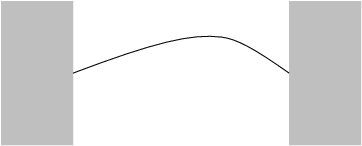
\epsfig{file={../fig/cordef}}}   
 \caption{The elevation of a clamped string verify a Laplace equation with
   Dirichlet boundary conditions.} 
 \label{figcordef}
\end{figure}

One can show that 
$\cal H$,
the space of functions zero in $0$ and $L$ is a Hilbert space for the scalar
product  $\mathrel{<} u,v \mathrel{>}=\int_0^L u(x)v(x) dx$.
(One speaks of {\bf Sobolev} space, see section \ref{secvafor}).
Moreover, one can show that the adjoint of $L$ is 
 $L^*=\frac{\partial^{2}}{\partial x^{2}}$:
\begin{equation}\label{eqadjoimq}
<Lu,v>=\int_0^l \frac{d^2u}{dx^2}vdx=
\int_0^lu\frac{d^2v}{dx^2}dx+[v\frac{du}{dx}-u\frac{dv}{dx}]^l_0 
\end{equation}
As $L^*=L$,  $L$ is called {\bf self-adjoint}.

\begin{figure}[htb]
 \centerline{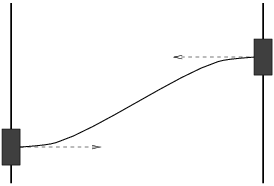
\epsfig{file={../fig/cordeg}}}   
 \caption{The elevation of a sliding string verify a Laplace equation with
   Neumann boundary conditions.}
 \label{figcordeg}
\end{figure}
One can also show that the space $\cal H_2$ of function with derivative zero
at $x=0$ and at $x=L$ is a Hilbert space for the scalar product: $\mathrel{<} u,v
\mathrel{>}=\int_0^Lu(x)v(x) dx$. 
Using equation \ref{eqadjoimq}, one shows that $L$ is also self-adjoint.

The form \index{form (definite)}
\begin{equation}
<Lu,u>=\int_o^l\frac{d^2u}{dx^2}udx=
[u\frac{du}{dx}]_0^l-\int_0^l(\frac{df}{dx})^2dx=
-\int_0^l(\frac{df}{dx})^2dx 
\end{equation}
is negative {\bf definite} in the case of the clamped string and negative (no
definite) in the case of the sliding string. Indeed, in this last case,
function $u=\mbox{ constant }$ makes  $<Lu,u>$ zero.

Let us conclude those remarks about boundary conditions by the compatibility
between the solution $u$ of a boundary problem
\begin{equation}
Lu=f
\end{equation}
and the right hand member $f$ \cite{ma:equad:Dautray1,ph:elect:VanBladel75}.

\begin{thm}
If there exists  a solution $v_0$ for the homogeneous adjoint problem :
\begin{equation}
L^*v_0=0
\end{equation}
then a necessary condition that the problem $Lu=f$ has a solution is that $f$
is orthogonal to  $v_0$. 
\end{thm}
\begin{pf}
Let us assume that $u_1$ is solution of:
\begin{equation}
Lu=f
\end{equation}
Then
\begin{equation}
\forall v,\ <v,Lu_1>=<v,f>
\end{equation}
thus 
\begin{equation}
\forall v,\ <L^*v,u_1>=<v,f>
\end{equation}
If there exists a function $v_0$ such that $L^*v_0=0$, then previous equation
implies: 
\begin{equation}
<v_0,f>=0
\end{equation}
\end{pf}

\begin{exmp}
In the case of the sliding string, function $v_0=1$ over $[0,L]$ is solution
of the homogeneous adjoint problem. The previous compatibility equation is then: $f$ should
be of average zero:
\begin{equation}
<v_0,f>=\int_0^lf dx.
\end{equation}
For the clamped string the homogeneous adjoint problem has no non zero
solution. 

\end{exmp}


\section{Linear boundary problems, integral methods}\label{chapmethint}
%%%%%%%%%%
\subsection{Green's function}
%%%%%%%%%%%%
Integral methods are used to solve linear boundary problems. Linearity is here
essential: the strategy consists in stating that if one knows the responses
$u_i$ of a physical linear system to entrances $f_i$, then one knows the
response of the system to an entry $f$ which is a sum $\sum c_i f_i$ (where
$c_i$ are real numbers).
Applications of this method can be found in the diffraction theory (see
section \ref{secdiffra}). Elementary solutions\footnote{Elementar
solutions correspond to Green functions in the case of translation
invariance (see section \ref{secresolinv}}  are intensively used in
electrostatic problems (see \ref{secpotelec}).
Consider (\cite{ph:elect:VanBladel75,ma:equad:Dautray1})
the following problem:
\begin{prob}\label{probpfppgreen} (Problem $P(f,\phi,\psi)$) :
Find $u\in U$ such that:
\begin{equation}
 Lu=f \mbox{ in } \Omega
\end{equation}
\begin{equation}
u=\phi \mbox{ in } \partial \Omega_1
\end{equation}
\begin{equation}
\frac{\partial u}{\partial n_{L}}=\psi \mbox{ in } \partial \Omega_2
\end{equation}
with $\partial \Omega_1 \cup\partial \Omega_2=\partial \Omega$.
\end{prob}
Let us find the solution using the Green method. Several cases exist:
\subsubsection{Nucleus zero, homogeneous problem}
%%%%%%%%%%%%%
\begin{defn}\label{defgreen}
The Green solution\index{Green solution} of problem $P(f,0,0)$ is the
function 
${\cal G}_y(x)$ solution of: 
\begin{equation}\label{eqdefgydy}
L{\cal G}_y=\delta_y
\end{equation}

The Green solution of the adjoint problem $P(f,0,0)$ is the function
${\cal G}^*_y(x)$ solution of 
\begin{equation}\label{eqdefgydyc}
\overline{L^*{\cal G}^*}_y=\delta_y
\end{equation}
where horizontal bar represents complex conjugation.
\end{defn}
\begin{thm}\label{theogreen}
If ${\cal G}_y$ and ${\cal G}^*_y$ exist then
$\overline{{\cal G}^*}_y(x)= {\cal G}_x(y)$
\end{thm}
\begin{pf}
By definition of the adjoint operator $L^*$ of an operator $L$
\begin{equation}
\int \overline{L^*{\cal G^*}}_y(r){\cal G}_x(r)dr= \int \overline{{\cal
G^*}}_{y}(r)L{\cal G}_x(r) dr
\end{equation}
Using equations \ref{eqdefgydy} and \ref{eqdefgydyc} of definition
\ref{defgreen} 
for ${\cal G}_y$ and ${\cal G}^*_y$,
one achieves the proof of the result.
\end{pf}
In particular, if $L=L^*$ then ${\cal G}^*_x(y)= {\cal G}_x(y)$.

\begin{thm}
There exists a unique function ${\cal G}_y$ such that
\begin{equation}
u(y)=\int {\cal G}_x(y) f(x)dx
\end{equation}
is solution of Problem $P(f,0,0)$ and
\begin{equation}
L{\cal G}_y=\delta_y
\end{equation}
\end{thm}
Proof\footnote{In particular, proof of the existence of ${\cal G}_y$.} of
this result is not given here but note that if 
${\cal G}_y$ exists then:
\begin{equation}
u(y)=\int \delta_y(x)u(x)=\int \overline{L^*{\cal G}^*}_y(x) u(x)dx.
\end{equation}
Thus, by the definition of the adjoint operator of an operator $L$:
\begin{equation}
u(y)=\int \bar{\cal G}^*_y(x) Lu(x)dx.
\end{equation}
Using equality $Lu=f$, we obtain:
\begin{equation}
u(y)=\int \bar{\cal G}^*_y(x) f(x),
\end{equation}
and from theorem \ref{theogreen} we have:
\begin{equation}
u(y)=\int {\cal G}_x(y) f(x)dx
\end{equation}
This last equation allows to find the solution of boundary problem, for any
function $f$, once Green function ${\cal G}_x(y)$ is known.

\subsubsection{Kernel zero, non homogeneous problem}
%%%%%%%%%%%%%
Solution of problem $P(f,\phi,\psi)$ is derived from previous Green functions:
\begin{equation}
u(y)=\int \delta_y(x)u(x)dx=\int \overline{L^*{\cal G^*}}_y(x)u(x)dx.
\end{equation}
Using Green's theorem, one has:
\begin{equation}
u(y)=\int \bar{\cal G}^*_y(x) Lu(x)dx
+\int_\Gamma  (\bar{\cal G}^*_y(x)\frac{\partial u}{\partial
n}(x)-u(x)\frac{\partial \bar{\cal G}^*_y}{\partial n}(x))dx,
\end{equation}
Using boundary conditions and theorem \ref{theogreen}, we get:
\begin{equation}
u(y)=\int {\cal G}_x(y) f(x)dx+\int_\Gamma  ({\cal
G}_x(y)\phi(x)-\psi(x)\frac{\partial {\cal G}_x(y)}{\partial n})dx, 
\end{equation}
This last equation allows to find the solution of problem
$P(f,\phi,\psi)$, for any triplet $(f,\phi,\psi)$, once Green function
${\cal G}_x(y)$ is known.


\subsubsection{Non zero kernel, homogeneous problem}
%%%%%%%%%%%%%
Let's recall the result of section \ref{secchoixesp} :
\begin{thm}
If  $L^*u_0=0$ has non zero solutions, and if $f$ isn't in the orthogonal of
$\mbox{ Ker }(L^*)$, the problem $P(f,0,0)$ has no solution.
\end{thm}
\begin{pf}
Let $u$ such that $Lu=f$. Let $v_0$ be a solution of
$L^*v_0=0$ ({\it i.e} a function of 
$\mbox{ Ker }(L^*)$).
Then:
\begin{eqnarray}
 \mathrel{<} f|v_0\mathrel{>} &=& \mathrel{<} Lu,v_0\mathrel{>}  \nonumber\\
       &=& \mathrel{<} u,L^*v_0\mathrel{>}.
\end{eqnarray} 
Thus $ \mathrel{<} f|v_0\mathrel{>} =0$
\end{pf}

However, once $f$ is projected onto the orthogonal of $\mbox{ Ker }(L^*)$, 
calculations similar to the previous ones can be made: Let us assume that the
kernel of $L$ is spanned by a function $u_0$ and that the kernel of
$L^*$ is spanned by $v_0$.
\begin{defn}\label{defgreen2}
The Green solution of problem $P(f,0,0)$ is the function
${\cal G}_y(x)$ solution of
\begin{equation}
L{\cal G}_y=\delta_y-u_0(y)u_0
\end{equation}
The Green solution of adjoint problem $P(f,0,0)$ is the function
${\cal G}^*_y(x)$ solution of
\begin{equation}
\overline{L^*{\cal G}^*}_y=\delta_y-v_0(y)v_0
\end{equation}
where horizontal bar represents complex conjugaison.
\end{defn}
\begin{thm}\label{theogreen2}
If ${\cal G}_y$ and ${\cal G}^*_y$ exist, then
$\overline{{\cal G}^*}_y(x)= {\cal G}_x(y)$
\end{thm}
\begin{pf}
By definition of the adjoint $L^*$ of an operator $L$
\begin{equation}
\int \overline{L^*{\cal G^*}}_y(r){\cal G}_x(r)dr=\int \overline{{\cal G^*}}_{y}(r)L{\cal G}_x(r)dr
\end{equation}
Using definition relations \ref{defgreen2}
of ${\cal G}_y$ and ${\cal G}^*_y$, one obtains the result.
\end{pf}
In particular, if $L=L^*$ then ${\cal G}^*_x(y)= {\cal G}_x(y)$.
\begin{thm}
There exists a unique function ${\cal G}_y$ such that
\begin{equation}
u(y)=\int {\cal G}_x(y) f(x)dx
\end{equation}
is solution of problem $P(f,0,0)$ in $\mbox{Ker}(L)^\perp$ and
\begin{equation}
L{\cal G}_y=\delta_y-u_0(y)u_0
\end{equation}
\end{thm}
Proof\footnote{In particular, the existence of  ${\cal G}_y$.} of this
theorem is not given here. However, let us justify 
solution definition formula. Assume that ${\cal G}_y$ exists.
Let $u_c$ be the projection of a function $u$ onto $\mbox{Ker}(L)^\perp$.
\begin{equation}
u_c(y)=u(y)-u_0(y)\int \bar{u}_0(x)u(x) dx.
\end{equation}
This can also be written:
\begin{equation}
u_c(y)=\int \delta_y(x)u(x)-u_0(y)\int \bar{u}_0(x)u(x) dx,
\end{equation}
or
\begin{equation}
u_c(y)=\int \overline{L^*{\cal G}^*}_y(x) u(x)dx=\int \bar{\cal G}^*_y(x) Lu(x)dx=\int \bar{\cal G}^*_y(x) f(x).
\end{equation}
From theorem \ref{theogreen2}, we have:
\begin{equation}
u_c(y)=\int {\cal G}_x(y) f(x)dx.
\end{equation}

\subsection{Resolution}\label{secresolinv}
%%%%%%%%%%%%%%%%%%%%%%%%%%
Once problem's Green function is found, problem's solution is obtained by
simple integration. Using of symmetries allows to simplify seeking of Green's
functions. 

\subsubsection{Images method}\index{images method}\label{secimage}
%%%%%%%%%
Let  $U$ be a domain having a symmetry plan: $\forall x
\in U, -x\in U$. Let $\partial U$ be the border of $U$.
Symmetry plane shares $U$ into two subdomains: $U_1$ and
$U_2$ (voir la figure \ref{figsymet}).
\begin{figure}[htb]
 \centerline{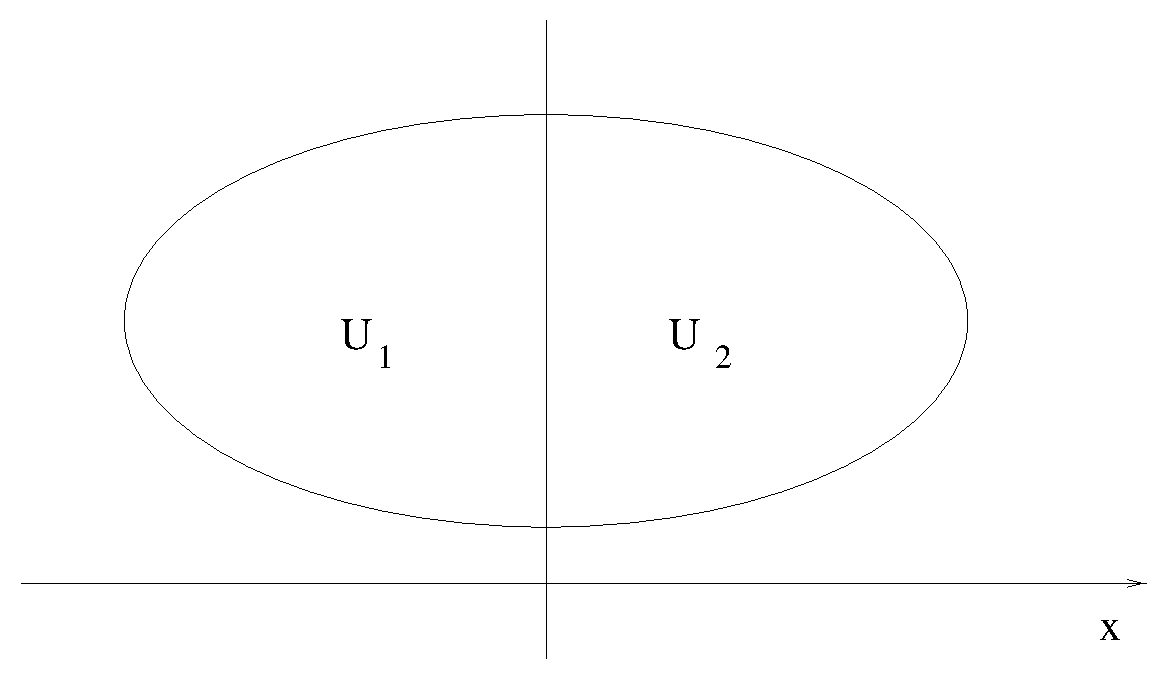
\epsfig{file={../fig/symet}}}   
 \caption{Domain $U$ is the union of $U_1$ and  $U_2$
symetrical with respect to plane $x=0$.}
 \label{figsymet}
\end{figure}
Let us seek the solution of the folowing problem:
\begin{prob}\label{probori} 
Find $G_y(x)$ such that:
\begin{equation}
LG_y(x)=\delta(x) \mbox{ in } U_1
\end{equation}
and
\begin{equation}
 G_y(x)=0 \mbox{  on  } \partial U_1
\end{equation}
\end{prob}
knowing solution of problem
\begin{prob}\label{probconnu}
Find $G^U_y(x)$ such that:
\begin{equation}
LG^U_y(x)=\delta(x) \mbox{  in  } U
\end{equation}
and
\begin{equation}
 G^U_y(x)=0 \mbox{  on  } \partial U
\end{equation}
\end{prob}
Method of solving problem \ref{probori} by using solution of problem
\ref{probconnu} is called images method \cite{ma:equad:Dautray1}.
Let us set ${\cal G}_y(x)={G}^U_y(x)-{G}^U_y(-x)$. Function ${\cal
G}_y(x)$ verifies
\begin{equation}
L{\cal G}_y(x)=\delta(x) \mbox{ in } U_1
\end{equation}
and
\begin{equation}
{\cal G}_y(x)=0 \mbox{  on  } \partial U_1
\end{equation}
Functions ${\cal G}_y(x)$ and $G_y(x)$ verify the same equation. Green
function $G_y(x)$ is thus simply the
restriction of function ${\cal G}_y(x)$ to $U_1$.
Problem \ref{probori} is thus solved.

\subsubsection{Invariance by translation}
%%%%%%
When problem $P(f,0,0)$ 
is invariant by translation, Green function's definition relation can be
simplified. Green function ${\cal G}_y(x)$ becomes a function ${\cal
  G}(x-y)$ that depends
only on difference $x-y$ and its definition relation is:
\begin{equation}
u(x)=\int {\cal G}(x-y)f(y)dx={\cal G}*f
\end{equation}
where $*$ is the convolution product (see appendix{appendconvoldist})\index{convolution}. Function ${\cal G}$ is in this case called
elementary solution and noted $e$.
Case where $P(f,0,0)$ is translation invariant typically corresponds to
infinite boundaries\cite{ma:distr:Schwartz65}. 
Here are some examples of well known elemantary solutions:
\begin{exmp}
{\bf Laplace equation in $R^3$.} Considered operator is:
\begin{equation}
L=\Delta
\end{equation}
Elementary solution is:
\begin{equation}
e(r)=\frac{1}{4\pi r}
\end{equation}
\end{exmp}
\begin{exmp}
{\bf Helmholtz equation in $R^3$.} Considered operator is: 
\begin{equation}
L=\Delta+k^2
\end{equation}
Elementary solution is:
\begin{equation}
e(r)=\frac{e^{jkr}}{4\pi r}
\end{equation}
\end{exmp}



\section{Boundary problems, variational methods}\label{chapmetvar}
%%%%%%%%%%%%%%%%%%%%%%
\subsection{Variational formulation}\label{secvafor}
%%%%%%%%%%%%%%
Let us consider a boundary problem:
\begin{prob}
Find $u\in U$ such that:
\begin{equation}\label{eqLufva}
Lu(x)=f(x) \forall x \in\Omega
\end{equation}
\begin{equation}
u(x)=g(x) \forall x\in\partial\Gamma
\end{equation}
\end{prob}
Let us suppose that is a unique solution $u$ of this problem.
For a functional space $V$ sufficiently large the previous problem, may be
equivalent to the following:
\begin{prob}
Find $u\in U$ such that:
\begin{equation}\label{eqvari}
\forall v\in V, <v|Lu>=<v|f>
\end{equation}
\end{prob}
This is the variational form of the boundary problem. To obtain the equality
\ref{eqvari}, we have just multiplied scalarly by a ``test function'' $<v|$
equation \ref{eqLufva}. 
A ``weak form'' of this problem can be found using Green formula type
formulas: the solution space is taken larger and as a counterpart, the test
functions space is taken smaller. let us illustrate those ideas on a simple
example:
\begin{exmp}
Find $u$ in $U=C^2$ such that:
\begin{equation}
-\Delta u=f, \forall x\in \Omega
\end{equation}
\begin{equation}
u=g, \forall x\in\partial\Omega
\end{equation}
The variational formulation is:
Find $u$ in $U=C^2$ such that:
\begin{equation}
\forall v\in V_1, -\int v\Delta u dx=\int vf dx
\end{equation}
Using the Green equality (see
appendix\ref{secappendgreeneq})\index{Green formula} and the
boundary conditions we can reformulate the problem in: 
find $u\in V$, such that:
\begin{equation}
\forall v\in V \int \partial_i v\partial_i u dx=\int vf dx
\end{equation}
One can show that this problem as a unique solution in $V=H^1_0(\Omega)$ where 
\begin{equation}
H^1(\Omega)=\{v\in L^2(\Omega);\partial_iv\in L^2(\Omega), 1\leq i\leq n\}
\end{equation}
is the Sobolev space of order 1 on $\Omega$ and $H_0^1(\Omega)$ is the
adherence of $H^1(\Omega)$ in the space ${\cal D}(\Omega)$ (space of
infinitely differentiable functions on $\Omega$, with compact support
in $\Omega$). 
\end{exmp}
It may be that, as for the previous example, the solution function
space and the test 
function space are the same. This is the case for most of linear operators $L$
encountered in physics. In this case, one can associate to $L$ a bilinear form
$a$. The (weak) variational problem is thus:
\begin{prob}\label{provari2} 
Find $u\in V$ such that 
\begin{equation}
\forall v\in V, a(u,v)=L(v)
\end{equation}
\end{prob}
\begin{exmp}
In this previous example, the bilinear form is:
\begin{equation}
a(u,v)=\int_\Omega \partial_i u(x)\partial_i v(x) dx.
\end{equation}

\end{exmp}
There exist theorems (Lax-Milgram theorem for instance) that proove the
existence and unicity of the solution of the previous problem
\ref{provari2} , under certain 
conditions on the bilinear form $a(u,v)$.

\subsection{Finite elements approximation}\label{secvarinum}
%%%%%%%%%%%%%%%%%%%%%%%%%%%%%

Let us consider the problem \ref{provari2} :
\begin{prob}
Find $u\in V$ such that: 
\begin{equation}
\forall v\in V, a(u,v)=L(v)
\end{equation}
\end{prob}
The method of approximation consists in choosing a finite dimension subspace
$V_h$ of $V$ and the problem to solve becomes:
\begin{prob}\label{provari3} 
Find $u_h\in V_h$ such that 
\begin{equation}
\forall v_h\in V_h, a(u_h,v_h)=L(v_h)
\end{equation}
\end{prob}
A base of $\{v_h^i\}$ of $V_h$ is chosen to satisfy boundary conditions.
The problem is reduced to finding the components of $u_h$:
\begin{equation}
u_h=\sum_i<v_h^i|u_h>v_h^i
\end{equation}
If $a$ is a bilinear form
\begin{equation}
a(u_h,v_h^i)=\sum_j<v_h^i|u_h>a(v_h^j,v_h^i),
\end{equation}
and to find the $<v_h^i|u_h>$'s is equivalent to solve a linear system (often
close to a diagonal system)that can be solved by classical algorithms 
\cite{ma:equad:Ciarlet88,ma:compu:Press92}
which can be direct methods 
(Gauss,Cholesky) or iterative (Jacobi, Gauss-Seidel,
relaxation). Note that if the vectors of the basis of $V_h$ are eigenvectors
of $L$, then the solving of the system is immediate (diagonal system). This is
the basis of the spectral methods for solving evolution problems. If $a$ is
not linear, we have to solve a 
nonlinear system. Let us give an example of a basis $\{v_h^i\}$.

\begin{exmp}
When $V=L^2([0,1])$, an example of  $V_h$ that can be chosen
\cite{ma:equad:Ciarlet88} is the set of piecewise-linear continuous functions
that are zero in $x=0$ and $x=1$ (for Dirichlet boundary conditions).
More precisely,  $L^2[0,1]$ can be approximated by the space of piecewise
linear continuous functions on intervals $[i/n,(i+1)/n]$, $i$ 
going from zero to
$n-1$, that are zero in $x=0$ and $x=1$. The basis of such a space is made by
functions  $(v_h^i), i\in
(1,\dots,n-1)$ defined by: 
\begin{equation}
v_h^i(x)=\frac{i-1}{n}+nx\mbox{ in  } [(i-1)/n,i/n]
\end{equation}
\begin{equation}
v_h^i(x)=\frac{i}{n}-nx\mbox{ in  }  [i/n,(i+1)/n]
\end{equation}
and zero anywhere else (see figure \ref{figapproxesp}).
\begin{figure}[htb]
 \centerline{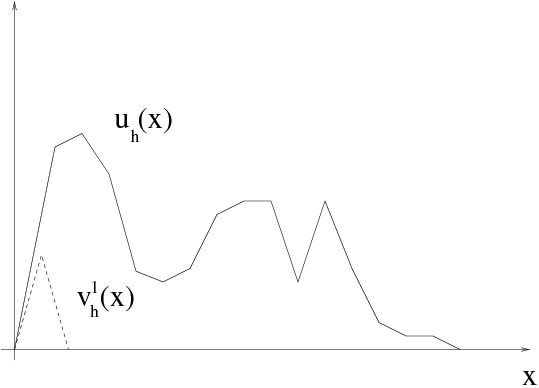
\epsfig{file={../fig/approxesp}}}   
 \caption{Space $L^2[0,1]$ can be approximated by pice wise linear continuous functions.}
 \label{figapproxesp}
\end{figure}
\end{exmp}

\subsection{Finite difference approximation}
%%%%%%%%%%%%%%%%%%%%%%%%%%%%%%%
Finite difference method is one of the most basic method to tackle PDE
problems. It is not strictly speaking a variational approximation. It is rather
a sort of variational method where weight functions $w_k$ are Dirac
functions $\delta_k$. Indeed,
when considering the boundary problem,
\begin{equation}\label{eqfini}
Lu=f \mbox{  for  }x\in \Omega
\end{equation}
instead of looking for an approximate solution $u_h$ which can be decomposed
on a basis of weight functions $w_k$:
\begin{equation}
u_h=\sum_k<w_k|u_h>w_k,
\end{equation}
the action of $L$ on $u$ is directly expressed in terms of Dirac functions, as
well as the right hand term of equation \ref{eqfini}:
\begin{equation}\label{eqfini2}
\sum (Lu)_{ik} \delta_k=\sum f_k\delta_k
\end{equation}
\begin{rem}
If $L$ contains
derivatives, the following formulas are used :
right formula, order 1:
\begin{equation}
\Delta x\frac{du}{dx}=\sum (u_{i+1}-u_i)\delta_i
\end{equation}
\begin{equation}
\Delta x^2\frac{d^2u}{dx^2}=\sum (u_{i+1}-2u_i+u_{i+1})\delta_i
\end{equation}
right formula order 2:
\begin{equation}
2\Delta x\frac{du}{dx}=\sum (-u_{i+2}+4u_{i+1}-3u_i)\delta_i
\end{equation}
\begin{equation}
\Delta x^2\frac{d^2u}{dx^2}=\sum (-u_{i+3}+4u_{i+2}-5u_{i+1}+2u_i)\delta_i
\end{equation}
Left formulas can be written in a similar way. Centred formulas, second order
are:
\begin{equation}
2\Delta x\frac{du}{dx}=\sum (u_{i+1}-u_{i-1})\delta_i
\end{equation}
\begin{equation}
\Delta x^2\frac{d^2u}{dx^2}=\sum (u_{i+1}-2u_{i}+u_{i-1})\delta_i
\end{equation}
Centred formulas, fourth order are:
\begin{equation}
12\Delta x\frac{du}{dx}=\sum (-u_{i+2}+8u_{i+1}-8u_{i-1}+u_{i-2})\delta_i
\end{equation}
\begin{equation}
12\Delta x^2\frac{d^2u}{dx^2}=\sum
(-u_{i+2}+16u_{i+1}-30u_i+16u_{i-1}-u_{i-2})\delta_i 
\end{equation}
\end{rem}
One can show that the equation \ref{eqfini2} is equivalent to the system of
equations:
\begin{equation}\label{eqfini3}
\sum_i (Lu)_{ik} =f_k
\end{equation}
One can see immediately that equation \ref{eqfini2} implies equation
\ref{eqfini3} in choosing ``test'' functions $v_i$ of support
$[x_i-1/2,x_i+1/2]$ and such that $v_i(x_i)=1$.


\subsection{Minimization problems}
%%%%%%%%%%%%%%%%%%%%%%%%%%%
A minimization problem can be written as follows:
\begin{prob}\label{promini}
Let $V$ a functional space, a $J(u)$ a functional.
Find $u\in V$, such that:
\begin{equation}
J(u)=\min_{v\in V} J(v)
\end{equation}
\end{prob}
The solving of minimization problems depends first on the nature of the
functional $J$ and on the space $V$.

As usually, the functional $J(u)$ is often approximated by a function of
several variables $J(u_1,\dots,u_N)$ where the $u_i$'s are the coordinate of
$u$ in some base $E_i$ that approximates $V$.
The methods to solve minimization problems can be classified into two
categories: 
One can distinguish problems without constraints (see
Fig.\ref{figcontraintesans}) and problems with constraints (see
Fig.\ref{figcontrainteavec}).
Minimization problems without constraints can be tackled theoretically by the
study of the zeros of the differential function $dF(u)$ if
exists. Numerically it can be less expensive to use dedicated methods. There
are methods that don't use derivatives of $F$ (downhill simplex method,
direction-set method) and methods that use derivative of $F$ (conjugate
gradient method, quasi-Newton methods). Details are given in 
\cite{ma:compu:Press92}.

Problems with constraints reduce the functional space $U$ to a set $V$ of
functions that satisfy some additional conditions.
Note that those sets $V$ are not vectorial spaces: a linear
combination of vectors of $V$ are not always in $V$. Let us give some example
of  constraints:
Let $U$ a functional space.
Consider the space
\begin{equation}
V=\{v\in U, \phi_{i}(v)=0, i\in 1,\dots,n \}
\end{equation}
where $\phi_{i}(v)$ are $n$ functionals. This is a first example of
constraints. It can be solved theoretically by using Lagrange
multipliers \cite{ma:equad:Ciarlet88},\index{constraint}. 
A second example of constraints is given by
\begin{equation}
V=\{v\in U, \phi_{i}(v)\leq 0, i\in 1,\dots,n  \}
v\end{equation}
where $\phi_{i}(v)$ are $n$ functionals.
The linear programming (see example \ref{exmplinepro}) problem is an example
of minimization problem with such constraints (in fact a mixing of equalities
and inequalities constraints).

\begin{figure}[htb]
 \centerline{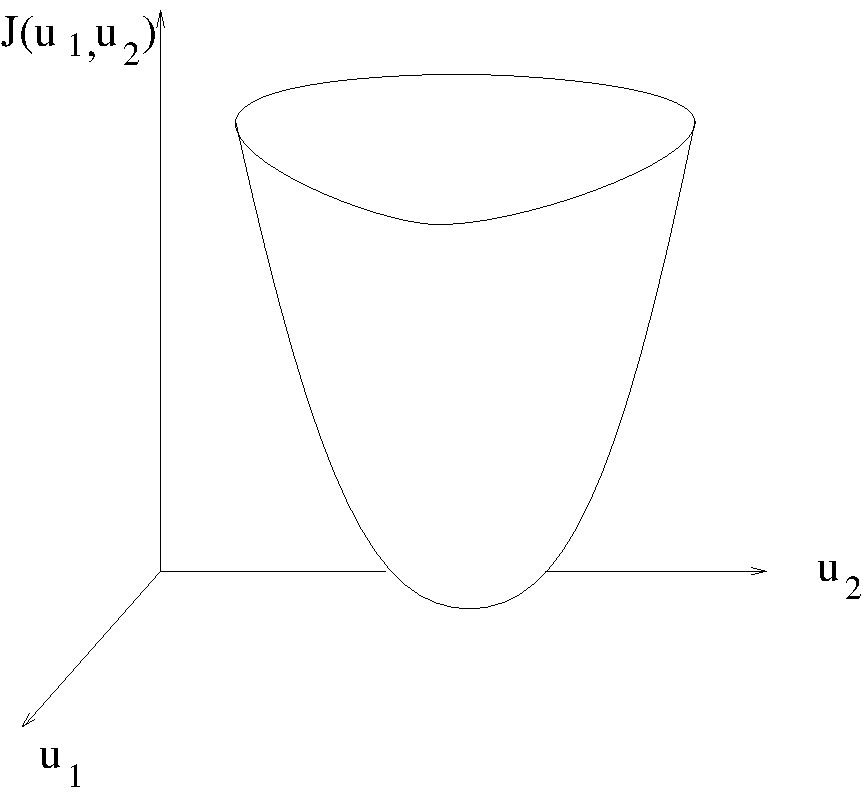
\epsfig{file={../fig/contraintesans}}}   
 \caption{Minimization of a function of two variables.}
 \label{figcontraintesans}
\end{figure}
\begin{figure}[htb]
 \centerline{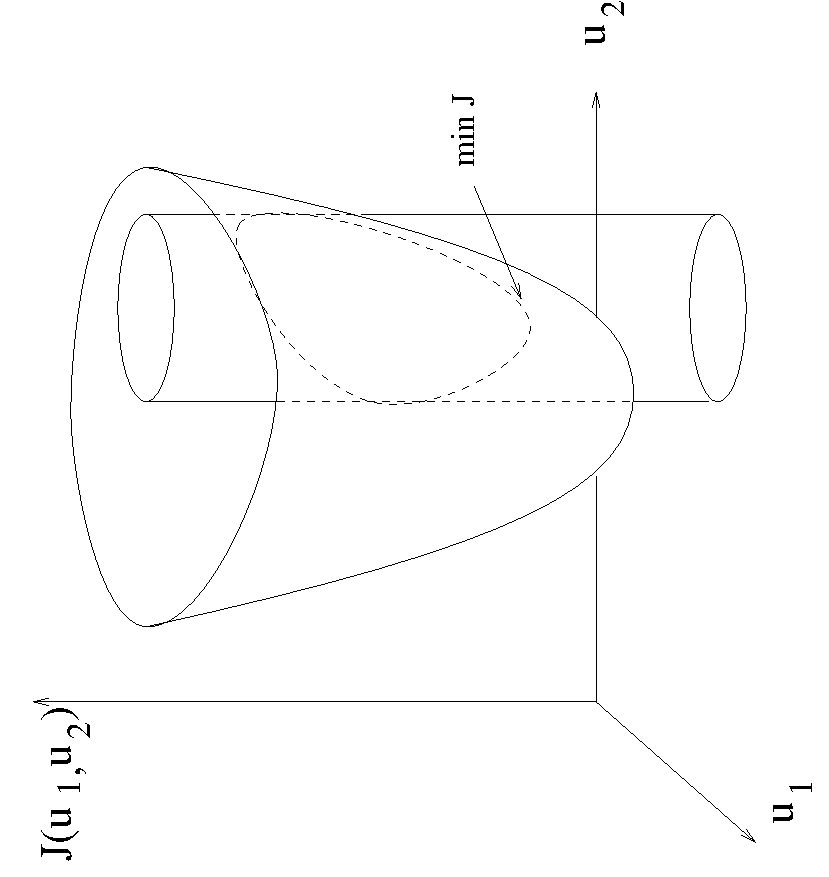
\epsfig{file={../fig/contrainteavec}}}   
 \caption{Minimization of a function of two variables with
 constraints. Here, space
   is reduced to a disk in the plane $u_1,u_2$. }
 \label{figcontrainteavec}
\end{figure}
\begin{figure}[htb]
 \centerline{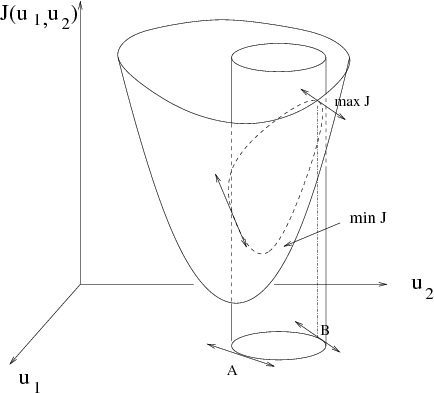
\epsfig{file={../fig/contrainteaveclag}}}   
 \caption{Illustration of the Lagrange multiplier. At point $A$ tangent vector on the surface and on the constraint curve are not paralele: $A$ does not correspond to an extremum. At point $B$ both tangent vector are colinear: we have an extremum.}
 \label{figcontrainteaveclag}
\end{figure}

\begin{exmp}
Let us consider of a first class of functional $J$ that are important for PDE
problems. 
Consider again the bilinear form introduced at section \ref{secvafor}.
If this bilinear form  $a(u,v)$ is symmetrical, {\it i.e.}
\begin{equation}
\forall u\in V, \forall v\in V, a(u,v)=a(v,u).
\end{equation}
the problem can be written as a minimization problem by introducing the functional:
\begin{equation}
J(v)=\frac{1}{2}a(v,v)-L(v)
\end{equation}
One can show that (under certain conditions) solving the variational problem:\\
Find $u\in V$ such that: 
\begin{equation}
\forall v\in V, a(u,v)=L(v)
\end{equation}
is equivalent to solve the minimization problem:\\
Find $u\in V$, such that:
\begin{equation}
J(u)=\min_{v\in V} J(v)
\end{equation}

\end{exmp}

Physical principles have sometimes a natural variational formulation (as
natural as a PDE formulation).
We will come back to the variational formulations at the section on least
action principle (see section  \ref{secprinmoindreact} ) and at the section
\ref{secpuisvirtu} on the principle of virtual powers.

\begin{exmp}\label{exmplinepro}
Another example of functional is given by the linear programming problem. Let
us consider a function $u$ that can be located by its coordinates
$u_i$ in a basis
$e_i$, $i\in \{1,dots,N\}$:
\begin{equation}
u=\sum u_ie_i
\end{equation}
In linear programming, the functional to minimize can be written  
\begin{equation}
F(u)=\sum c_iu_i
\end{equation}
and is subject to $N$ primary constraints:
\begin{equation}
\forall i, u_i\geq 0
\end{equation}
and $M=m_1+m_2+m_3$ additional constraints:
\begin{equation}
k\in\{1,\dots,m_1\}, \sum_j a_{k,j}u_j\leq b_k, (b_k\geq 0)
\end{equation}
\begin{equation}
k\in\{m_1+1,\dots,m_1+m_2\}, \sum_j a_{k,j}u_j\geq b_k\geq 0
\end{equation}
\begin{equation}
k\in\{m_1+m_2+1,\dots,m_1+m_2+m_3\}, \sum_j a_{k,j}u_j=b_k\geq 0
\end{equation}
The numerical algorithm to solve this type of problem is presented in
\cite{ma:compu:Press92}. It is called the simplex method.
\end{exmp}

\begin{exmp}\label{exmpsimul}
When the variables $u_i$ can take only discrete values, one speaks about
discrete or combinatorial optimization. The function to minimize can be for
instance (travelling salesman problem):
\begin{equation}
J(u,v)=\sum_{i=1}^N \sqrt{(u_{\sigma(i)}-u_{\sigma(i-1)})^2+
  (v_{\sigma(i)}-v_{\sigma(i-1)})^2} 
\end{equation}
where $u_i,v_i$ are the coordinates of a city number $i$. The coordinates of
the cities are numbers fixed in advance but the order in which the $N$ cities
are visited ({\it i.e} the permutation $\sigma$ of $\{1,\dots, N\}$) is to be
find to minimize $J$. Simulated annealing is a method to solve this problem
and is presented in \cite{ma:compu:Press92}. 
\end{exmp}



\subsection{Lagrange multipliers}
%%%%%%%%%%%

Lagrange multipliers method is an interesting approach to solve the
minimization problem of a function of $N$ variables with constraints, {\it
  i. e. } to solve the following problem:
\index{contrainte}\index{Lagrange multiplier}
\begin{prob}
Find  $u$ in a space $V$ of dimension $N$ such that 
\begin{equation} 
F(u)=\min_{v\in V}F(v)
\end{equation}
with $n$ constraints, $R_i(x)=0, i=1,\dots,n.$
\end{prob}
Lagrange multipliers method is used in statistical physics (see section
\ref{chapphysstat}).
In a problem without any constraints, solution $u$ verifies:
\begin{equation}
dF=0
\end{equation}
In the case with constraints, the $n$ coordinates
$u_i$ of $u$ are not independent. Indeed, they should verify the relations:
\begin{equation}
dR_i=0
\end{equation}
Lagrange multipliers method consists in looking for $n$ numbers $\lambda_i$
called Lagrange multipliers such that:
\begin{equation}
dL=dF+\sum \lambda_i dR_i=0
\end{equation}
One obtains the following equation system:
\begin{equation}
\frac{\partial F}{\partial x_j}+\sum \lambda_i \frac{\partial R_i}{\partial x_j}=0
\end{equation}
\section{Linear evolution problems, spectral method}\label{chapmethspec}
%%%%%%%%%%%%%%%%%%%%%%%%%%%%%%%%
\subsection{Spectral point of view}
%%%%%%%%%%%%%%%%%%%%%%
Spectral method is used to solve linear evolution problems of type Problem
\ref{probevollin}. Quantum mechanics (see chapters \ref{chapmq} and
\ref{chapproncorps} ) supplies beautiful spectral problems
{\it via} Schr\"odinger equation.
Eigenvalues of the linear operator considered (the hamiltonian) are
interpreted as energies associated to states (the eigenfunctions of the
hamiltonian). Electromagnetism leads also to spectral problems (cavity
modes). 

Spectral methods consists in defining first the space where the operator $L$
of problem \ref{probevollin} acts
and in providing it with the Hilbert space structure. Functions that verify:
\begin{equation}
Lu_k(x)=\lambda_ku_k(x)
\end{equation}
are then seeked. Once eigenfunctions $u_{k(x)}$ are found,
the problem is reduced to integration of an ordinary differential equations
(diagonal) system.

The following problem is a particular case of linear evolution problem
\index{response (linear)} (one speaks about {\bf linear response} problem) 
\begin{prob} 
Find $\phi\in V$ such that:
\begin{equation}
\frac{d\phi}{dt}=(H_0+H(t))\phi
\end{equation}
where $H_0$ is a linear diagonalisable operator and $H(t)$ is a linear
operator ``small'' with respect to $H_0$.
\end{prob}
This problem can be tackled by using a spectral method. Section
\ref{secreplinmq} presents an example of linear response in quantum mechanics.


\subsection{Some spectral analysis theorems}
%%%%%%%%%%%%%%%%%%%%%%%%%%%%%
In this section, some results on the spectral analysis of a linear operator
$L$ are presented. Demonstration are given when $L$ is a linear operator
acting from a finite dimension space $E$ to itself. Infinite dimension case is
treated in specialized books (see for instance \cite{ma:equad:Dautray5}). 
let $L$ be an operator acting on $E$.
The spectral problem associated to $L$ is:
\begin{prob}
Find non zero vectors $u\in V$ (called eigenvectors) and numbers $\lambda$
(called eigenvalues) such that: 
\begin{equation}
Lu=\lambda u
\end{equation}
\end{prob}
Here is a fundamental theorem:
\begin{thm}
Following conditions are equivalent:
\begin{enumerate}
\item $\exists u \neq 0 \: Lu=\lambda u$
\item matrix  $L-\lambda I$ is singular
\item $det(L-\lambda I)=0$
\end{enumerate}
\end{thm}
A matrix is said diagonalisable if it exists a basis in which it has a
diagonal form \cite{ma:algeb:Strang76}.
\begin{thm}
If a squared matrix $L$ of dimension $n$ has $n$ eigenvectors linearly
independent, then $L$ is diagonalisable. Moreover, if those vectors are chosen
as columns of a matrix $S$, then:
\begin{equation}
\Lambda = S^{-1} L S \mbox{  with  } \Lambda \mbox{  diagonal  }
\end{equation}
\end{thm}
\begin{pf}
Let us write vectors $u_i$ as column of matrix $S$ and let let us calculate
$LS$: 
\begin{equation}
LS=L \left( \begin{array}{cccc}
              \vdots&\vdots& &\vdots\cr
               u_1&u_2&\ldots&u_n\cr 
              \vdots&\vdots& &\vdots\cr
\end{array} \right)
\end{equation}
\begin{equation}
=
\left( \begin{array}{cccc}
              \vdots&\vdots& &\vdots\cr
              \lambda_1 u_1&\lambda_2 u_2&\ldots&\lambda_n u_n\cr
              \vdots&\vdots& &\vdots\cr
\end{array} \right)
\end{equation}
\begin{equation}
\left( \begin{array}{cccc}
\vdots&\vdots& &\vdots\cr
              u_1&u_2&\ldots&u_n\cr
              \vdots&\vdots&
&\vdots\cr
\end{array} \right)
.
\left( \begin{array}{cccc}
\lambda_1& & &\cr
&\lambda_2&&\cr
&&\ddots&\cr
&&&\lambda_n
\end{array} \right)
\end{equation}
\begin{equation}
LS=S\Lambda
\end{equation}
Matrix $S$ is invertible since vectors $u_i$ are supposed linearly
independent, thus:
\begin{equation}
\lambda=S^{-1}LS
\end{equation}
\end{pf}
\begin{rem}\label{remmatrindep}
If a matrix $L$ has $n$ distinct eigenvalues then its eigenvectors are
linearly independent.
\end{rem}

Let us assume that space $E$ is a Hilbert space equiped by the scalar
product $< . | . >$.
\begin{defn}
Operator $L^*$ adjoint of $L$ is by definition defined by:
\begin{equation} 
\forall u, v   \mathrel{<} L^*u|v\mathrel{>} = \mathrel{<} u|Lv\mathrel{>} 
\end{equation}
\end{defn}
\begin{defn} 
An auto-adjoint operator is an operator $L$ such that $L=L^*$
\end{defn}
\begin{thm}
For each hermitic operator  $L$, there exists at least one basis constituted by
orthonormal eigenvectors. $L$ is diagonal in this basis and diagonal elements
are eigenvalues.
\end{thm}
\begin{pf}
Consider a space $E_n$ of dimension $n$.
Let  $|u_1\mathrel{>} $ be the eigenvector associated to eigenvalue $\lambda_1$ of
$A$. Let us consider a basis the space ($|u_1\mathrel{>} $ direct sum any basis of
$E^\perp_{n-1}$).
In this basis: 
\begin{equation}
L= 
\left( \begin{array}{cccc}
\lambda_1& &v& \cr
             0& & & \cr
             \vdots& &B& \cr
              0& & & \cr
\end{array} \right)
\end{equation}
The first column of $L$ is image of $u_1$.
Now, $L$ is hermitical thus:
\begin{equation}
L= 
\left( \begin{array}{cccc}
\lambda_1&0&\ldots&0 \cr
             0& & & \cr
             \vdots& &B& \cr
              0& & & \cr
\end{array} \right)
\end{equation}
By recurrence, property is prooved..
\end{pf}
\begin{thm}
Eigenvalues of an hermitic operator $L$ are real.
\end{thm}
\begin{pf}
Consider the spectral equation:
\begin{equation}
L|u\mathrel{>} =\lambda|u\mathrel{>} 
\end{equation}
Multiplying it by $ \mathrel{<} u|$, one obtains:
\begin{equation}
 \mathrel{<} u|Lu\mathrel{>} =\lambda \mathrel{<} u|u\mathrel{>} 
\label{uAu}
\end{equation}
Complex conjugated equation of \ref{uAu} is:
\begin{equation}
 \mathrel{<} u|L^*u\mathrel{>} =\lambda^* \mathrel{<} u|u\mathrel{>} 
\end{equation}
$ \mathrel{<} u|u\mathrel{>} $ being real and $L^*=L$, one has:
$\lambda=\lambda^*$ 
\end{pf}
\begin{thm}
Two eigenvectors $|u_1\mathrel{>} $ and $|u_2\mathrel{>} $ associated to two distinct
eigenvalues $\lambda_1$ and $\lambda_2$ of an hermitic operator are
orthogonal. 
\end{thm}
\begin{pf}
By definition:
\begin{equation}
L|u_1\mathrel{>} =\lambda_1|u_1\mathrel{>} 
\end{equation}
\begin{equation}
L|u_2\mathrel{>} =\lambda_2|u_2\mathrel{>} 
\end{equation}
Thus:
\begin{equation}
 \mathrel{<} u_2|Lu_1\mathrel{>} =\lambda_1 \mathrel{<} u_2|u_1\mathrel{>} 
\end{equation}
\begin{equation}
 \mathrel{<} u_1|Lu_2\mathrel{>} =\lambda_2 \mathrel{<} u_1|u_2\mathrel{>} 
\end{equation}
The difference between previous two equations implies:
\begin{equation}
0=(\lambda_1-\lambda_2) \mathrel{<} u_2|u_1\mathrel{>} 
\end{equation}
which implies the result.
\end{pf}
Let us now presents some methods and tips to solve spectral problems.

%%%%%%%%%%%%%%%%%%%%%%%%%%%%%%%%%%%%%%%%%%%%%%%%%%%%
\subsection{Solving spectral problems}\label{chapresospec}
%%%%%%%%%%%%%%%%%%%%%%%%%%%%%%%%%%%%%%%%%%%%%%%%%%%
The fundamental step for solving linear evolution problems by doing
the spectral 
method is the spectral analysis of the linear operator involved. It can be done
numerically, but two cases are favourable to do the spectral analysis by hand:
case where there are symmetries, and case where a perturbative approach is
possible. 
\subsubsection{Using symmetries}
%%%%%%%%%%%%%%%%%%%%%%%%%%%%
Using of symmetries rely on the following fundamental theorem:
\begin{thm}
If operator $L$ commutes with an operator $T$, then eigenvectors of $T$ are
also eigenvectors of $L$. 
\end{thm}
Proof is given in appendix \ref{chapgroupes}.
Applications of rotation invariance are presented at section \ref{secpotcent}.
Bloch's theorem deals with translation invariance (see theorem \ref{theobloch}
at section \ref{sectheobloch}).
\subsubsection{Perturbative approximation}
%%%%%%%%%%%%%%%%%%%%%%%%%%%%%%%%%%%%%%%%%%
A perturbative approach can be considered each time operator $U$ to
diagonalize can be considered as a sum of an operator $U^{0}$ whose spectral
analysis is known and of an operator $U^{1}$ small with respect to $U^{0}$.
The problem to be solved is then the 
following:\index{perturbation method}
\begin{equation} 
U\mid  \phi \mathrel{>}  = \lambda\mid  \psi \mathrel{>} \label{bod}
\end{equation}
Introducing the parameter $\epsilon$, it is assumed that $U$
can be expanded as:
\begin{equation} 
U=U_{0}+\epsilon U_{1}+\epsilon ^{2}U_2+...
\end{equation}
Let us admit\footnote{This is not obvious from a mathematical point of view
  (see~{Kato}~\cite{ma:equad:Kato66})} that the eigenvectors can be expanded
in $\epsilon$ :
For the  i$^{th}$ eigenvector:
\begin{equation} 
\mid \phi^{i}\mathrel{>} =\mid \phi^{i}_{0}\mathrel{>} +\epsilon
\mid \phi^{i}_{1}\mathrel{>} +\epsilon^{2}\mid \phi^{i}_{2}\mathrel{>} +...
\label{hyph} 
\end{equation}
Equation (\ref{bod}) defines eigenvector, only to a factor.
Indeed, if $\mid \phi^{i}\mathrel{>} $ is solution, then
$a\,e^{i\theta}\mid \phi^{i}\mathrel{>} $ is also solution. Let us fix the norm of
the eigenvectors to $1$. Phase can also be chosen. We impose that
phase of vector $\mid \phi^{i}\mathrel{>} $ is the phase of vector
$\mid \phi^{i}_0\mathrel{>} $.
Approximated vectors $\mid \phi^{i}\mathrel{>} $ and
$\mid \phi^{j}\mathrel{>} $ should be exactly orthogonal.
\begin{equation} 
\mathrel{<} \phi^{i}\mid \phi^{j}\mathrel{>} =0 
\end{equation}
Egalating coefficients of $\epsilon^k$, one gets:
\begin{equation}\label{eqortper}
\mathrel{<} \phi^{i}_{0}\mid \phi^{j}_{k}\mathrel{>} +\mathrel{<} \phi^{i}_{1}\mid
\phi^{j}_{k-1}\mathrel{>} +\ldots+\mathrel{<} \phi^{i}_{k}\mid
\phi^{j}_{0}\mathrel{>} =0 
\end{equation}
%
Approximated eigenvectors are imposed to be exactly normed and 
$\mathrel{<} \phi^{i}_{0}\mid \phi^{i}_{j}\mathrel{>} $ real:
\begin{equation} 
\mathrel{<} \phi^{i}_{0}\mid \phi^{i}_{1}\mathrel{>} =1 
\end{equation}
Equalating coefficients in $\epsilon^k$ with $k > 1$ 
in product
$\mathrel{<} \phi^{i}\mid \phi^{i}\mathrel{>} =1$, one gets:
\begin{equation}
\mathrel{<} \phi^{i}_{0}\mid \phi^{i}_{k}\mathrel{>} +\mathrel{<} \phi^{i}_{1}\mid
\phi^{i}_{k-1}\mathrel{>} +\ldots+\mathrel{<} \phi^{i}_{k}\mid \phi^{i}_{0}\mathrel{>} =0.
\end{equation}
Substituting those expansions into spectral equation \ref{bod} and equalating
coefficients of successive powers of $\epsilon$ yields to:
\begin{eqnarray}
&&U_{0}\mid \phi^{i}_{j}\mathrel{>} +U_{1}\mid \phi^{i}_{j-1}\mathrel{>} +...+U_{j}\mid \phi^{i}_{0}\mathrel{>} \nonumber\\
&=&\lambda_{0}^{i}\mid \phi^{i}_{j}\mathrel{>} +\lambda_{1}^{i}\mid \phi^{i}_{j-1}\mathrel{>} +...
+\lambda_{j}^{i}\mid \phi^{i}_{0}\mathrel{>}  \label{oivj}
\end{eqnarray}

Projecting previous equations onto eigenvectors at zero order, and using
conditions \ref{eqortper}, successive corrections to eigenvectors and
eigenvalues are obtained.

\subsubsection{Variational approximation}
%%%%%%%%%%%%%%%%%%%%%%%%%%%%%%
In the same way that problem
\begin{prob}
Find $u$ such that:
\begin{enumerate}
\item 
\begin{equation}
Lu=f, u\in E, x\in\Omega
\end{equation}
\item $u$ satisfies boundary conditions on the border
$\partial 
\Omega$ of $\Omega$.
\end{enumerate}
\end{prob}
can be solved by variational method, spectral problem:
\begin{prob}
Find $u$ and $\lambda$ such that:
\begin{enumerate}
\item 
\begin{equation}
Lu-\lambda u=f, u\in E, x\in\Omega
\end{equation}
\item $u$ satisfies boundary conditions on the border
$\partial \Omega$ of $\Omega$.
\end{enumerate}
\end{prob}
can also be solved by variational methods. In case where $L$ is self adjoint
and $f$ is zero (quantum mechanics case), problem can be reduced to a
{\bf minimization problem}. In particular, one can show that:
\begin{thm}
The eigenvector $\phi$ with lowest energy $E_0$  of self adjoint operator
$H$ is solution of problem:
Find $\phi$ normed such that:
\begin{equation}
J(\phi)=\min_{\psi\in V}J(\psi)
\end{equation}
where $J(\psi)=<\psi|H\psi>$. Eigenvalue associated to $\phi$
is $J(\phi)$.
\end{thm}
Demonstration is given in \cite{ph:mecaq:Cohen73,ph:mecaq:Pauling60}.
Practically, a family of vectors $v_i$ of $V$ is chosen and one hopes that
eigenvector $\phi$ is well approximated by some linear combination of those vectors:
\begin{equation}
\phi=\sum c_iv_i
\end{equation}
Solving minimization problem is equivalent to finding coefficients
$c_i$. At chapter 
\ref{chapproncorps}, we will see several examples of good choices of families
$v_i$. 
\begin{rem}
In variational calculations, as well as in perturbative calculations,
symmetries should be used each time they occur to simplify solving of
spectral problems (see chapter \ref{chapproncorps}).
\end{rem}


\section{Nonlinear evolution problems, perturbative
  methods}\label{partprobevolnl} 
%%%%%%%%%%%%%%%%%%%%%%%%%%%%%%
\subsection{Problem statement}
%%%%%%%%%%%%%%
Perturbative methods allow to solve nonlinear evolution problems. They are
used in hydrodynamics, plasma physics for solving nonlinear fluid models (see
for instance \cite{ph:plasm:Chen84}). 
Problems of nonlinear ordinary differential equations can also be solved by
perturbative methods (see for instance \cite{ma:equad:Arnold83} where
averaging method is presented).  
Famous KAM theorem (Kolmogorov--Arnold--Moser) gives important results about
the perturbation of hamiltonian systems. 
Perturbative methods are only one of the possible methods: geometrical
methods, normal form methods
\cite{ma:equad:Arnold83} can give good results. Numerical technics will be
introduced at next section.

Consider the following problem:
\begin{prob}\label{proeqp} 
Find $u\in V$ such that:
\begin{enumerate}
\item 
\begin{equation}
\frac{\partial u}{\partial t}=Lu+N(u), u\in E, x\in\Omega
\end{equation}
\item $u$ verifies boundary conditions on the border
$\partial 
\Omega$ of $\Omega$.
\item $u$ verifies initial conditions.
\end{enumerate}
\end{prob}
Various perturbative methods are presented now.
\subsection{Regular perturbation}
%%%%%%%%%%%%%%%%%%%%%%%%%%%%%%%%%
Solving method can be described as follows:
\begin{alg}
\begin{enumerate}
\item Differential equation is written as:
\begin{equation}
\frac{\partial u}{\partial t}=Lu+\epsilon N(u)
\end{equation}
\item The solution $u_0$ of the problem when $\epsilon$ is zero is known.
\item General solution is seeked as:
\begin{equation}
u(t)=\sum \epsilon^i u_i(t)
\end{equation}
\item Function $N(u)$ is developed around $u_0$ using Taylor type formula:
\begin{equation}
N(u_0+\epsilon u_1)=N(u_0)+\epsilon u_1\left.\frac{\partial N}{\partial
    u}\right)_{u_0} 
\end{equation}
\item A hierarchy of  {\bf linear} equations to solve is obtained:
\begin{equation}
\frac{\partial u_0}{\partial t}=Lu_0
\end{equation}
\begin{equation}
\frac{\partial u_1}{\partial t}=Lu_1+u_1\left.\frac{\partial N}{\partial
u}\right)_{u_0} 
\end{equation}
\end{enumerate}
\end{alg}
This method is simple but singular problem my arise for which solution is not
valid uniformly in $t$.
\begin{exmp}
{\bf Non uniformity of regular perturbative expansions} (see 
\cite{ma:equad:Bender87}). Consider Duffing equation:
\begin{equation}
\frac{d^2y}{dt^2}+y+\epsilon y^3=0
\end{equation}
Let us look for solution $y(t)$ which can be written as:
\begin{equation}
y(t)=y_0(t)+\epsilon y_1(t)+\epsilon^2 y_2(t)
\end{equation}
The linear hierarchy obtained with the previous assumption is:
\begin{eqnarray}
\frac{d^2y_0}{dt^2}+y_0&=&0\\
\frac{d^2y_1}{dt^2}+y_1&=&-y_0^3
\end{eqnarray}
With initial conditions : $y_0(0)=1,y'_0(0)=0$, one gets:
\begin{equation}
y_0(t)=cos(t)
\end{equation}
and a particular solution for $y_1$ will be unbounded\footnote{%%%%%%%%%
Indeed solution of equation:
\begin{equation}
\ddot y+y=cos t
\end{equation}
is
\begin{equation}
y(t)=A cos t+ B \sin t+\frac{1}{2}t \sin t
\end{equation}
}%%%%%%%%%%%
, now solution is expected to be bounded.
Indeed (see \cite{ma:equad:Bender87}), multiplying Duffing equation by $\dot
y$, one gets the following differential equation:
\begin{equation}
\frac{d}{dt}[\frac{1}{2}(\frac{dy}{dt})^2+
\frac{1}{2}y^2+\frac{1}{4}\epsilon y^4]=0.
\end{equation}
We have thus:
\begin{equation}
\frac{1}{2}(\frac{dy}{dt})^2+\frac{1}{2}y^2+\frac{1}{4}\epsilon
y^4=C
\end{equation}
where $C$ is a constant. Thus  $y^2$ is bounded if $\epsilon > 0$. 
\begin{rem}
In fact Duffing system is conservative.
\end{rem}
\end{exmp}
\begin{rem}
{\bf Origin of secular terms}: A regular perturbative expansion of a
periodical function whose period depends on a parameter gives rise
automatically to secular terms (see
\cite{ma:equad:Bender87}): 
\begin{equation}
\sin((1+\epsilon) t)=\sin(t)cos(\epsilon t)+\sin(\epsilon t).cos(t)
\end{equation}
\begin{equation}
=\\sin(t)(1+\frac{\epsilon^2t^2}{2}+\dots)+(\epsilon t+\dots).cos(t)
\end{equation}
\end{rem}
\subsection{Born's iterative method}
%%%%%%%%%%%%%%%%%%%%%%%%%%%%%%%%
\begin{alg}
\begin{enumerate}
\item Differential equation is transformed into an integral equation:
\begin{equation}
u=\int_0^t(Lu+N(u))dt'
\end{equation}
\item A sequence of functions $u_n$ converging to the solution $u$ is seeked: 
Starting from chosen solution $u_0$, successive
$u_n$ are evaluated using recurrence formula:
\begin{equation}
u_{n+1}=\int_0^t(Lu_n+N(u_n))dt'
\end{equation}
\end{enumerate}
\end{alg}
This method is more ``global'' than previous one 
\index{Born iterative method} and can thus suppress some
divergencies. It is used in diffusion problems
\cite{ph:mecaq:Cohen73,ph:mecaq:Cohen88}.  It has the drawback to allow less
control on approximations.
\subsection{Multiple scales method}
%%%%%%%%%%%%%%%%%%%%%%
\begin{alg}
\begin{enumerate}
\item Assume the system can be written as:
\begin{equation}\label{eqavece}
\frac{\partial u}{\partial t}=Lu+\epsilon N(u)
\end{equation}
\item Solution $u$ is looked for as:
\begin{equation}\label{eqdevmu}
u(x,t)=u_0(x,T_0,T_1,\dots,T_N)+\epsilon
u(x,T_0,T_1,\dots,T_N)+\dots+O(\epsilon^N) 
\end{equation}
with $T_n=\epsilon^n t$ for all $n\in \{0,\dots,N\}$.
\item A hierarchy of equations to solve is obtained by substituting
expansion \ref{eqdevmu} into equation \ref{eqavece}. 
\end{enumerate}
\end{alg}
For examples see \cite{ma:equad:Nayfeh95}.
\subsection{Poincar\'e-Lindstedt method}
%%%%%%%%%%%%%%%%%%
This method is closely related to previous one, but is specially dedicated to
studying periodical solutions.
Problem to solve should be:\index{Poincar\'e-Lindstedt}
\begin{prob}
Find $u$ such that:
\begin{equation}\label{eqarespo}
G(u,\omega)=0
\end{equation}
where $u$ is a periodic function of pulsation $\omega$. Setting $\tau=\omega
t$, one gets:
\begin{equation}
u(x,\tau +2\pi)=u(x,\tau)
\end{equation}
\end{prob}
Resolution method is the following:
\begin{alg}
\begin{enumerate}
\item Existence of a solution $u_0(x)$ which does not depend on $\tau$ is
  imposed: 
\begin{equation}
G(u_0(x),\omega)=0
\label{fix}
\end{equation}
\item 
Solutions are seeked as:
\begin{equation}
u(x,\tau,\epsilon)=u_0(x)+\epsilon
u_1(x,\tau)+\frac{\epsilon^2}{2}u_2(x,\tau)+\dots
\label{form1}
\end{equation}
\begin{equation}
\omega(\epsilon)=\omega_0+\epsilon\omega_1+\frac{\epsilon}{2}\omega_2
\label{form2}
\end{equation}
with  $u(x,\tau,\epsilon=0)=u_0(x)$.
\item A hierarchy of linear equations to solve is obtained by expending $G$ around $u_0$and substituting \ref{form1} and \ref{form2} into \ref{eqarespo}.
\end{enumerate}
\end{alg}


\subsection{WKB method}\label{mathsecWKB}
%%%%%%%%%%%%%%%%%%%%%%%%%%
 WKB (Wentzel-Krammers-Brillouin) method is also a perturbation
method. It will be presented at section
\ref{secWKB} in the proof of ikonal equation.



\section{Evolution, numerical time integration}\label{annexnum}
%%%%%%%%%%%%%%%%%%%%%%%%%%%%%%%%
\subsection{Introduction}
%%%%%%%%%%%%%%%%%%%
There exist very good books 
(see \cite{ma:compu:garcia94,ma:compu:Press92,ma:compu:Parker89}) 
about numerical integration of PDE evolution problem. Note that all methods
(finite difference, finite element, spectral methods) contains as a final step
the time integration of a ODE system. In this section this time integration is
treated.  Problem to be solved is the following
\begin{prob}\label{probmathevovec} (Cauchy problem)
Find functions
$u_k(t)$ obeying the ODE system
\begin{equation}
\frac{d u_k}{dt}=F_k(u_h,t)
\end{equation}
where $u_h(x,t=0)$ is known. 
\end{prob}
We will not present here details about stability and precision calculation of
the numerical integration schemes, however the reader should always keep in
mind this crucial problem. Generally speaking, knowledge
of mathematical properties of solutions should always be used to verify
numerical results. For instance, if the solution of problem
\ref{probmathevovec} is known to be bounded, and that the solution obtained
numerically diverges, then numerical solution will be obviously considered as
bad. This problem of stability is the first that the numerician meet. However,
more refined considerations have to be considered. Integrals of movement are a
classical way to check accuracy of solutions. For hamiltonian systems for
instance, energy conservation should be checked at regular time intervals.

\subsection{Euler method}
%%%%%%%%%%%%%%%%%%%%%%%%%%%%%%
Euler method consists in approximating the time derivative
\begin{equation}
\frac{du_k}{dt}
\end{equation}
by
\begin{equation}
\frac{1}{\Delta t}(u_{k,t+1}-u_{k,t}).
\end{equation}
However, the way the right-hand term is evaluated is very important for the
stability of the integration scheme
\cite{ma:compu:Press92}. So, explicit scheme:
\begin{equation}
\frac{1}{\Delta t}(u_{k,t+1}-u_{k,t})=F_i(u_t)
\end{equation}
is unstable if $F=\frac{\partial u}{\partial x}$. On another hand, implicit
scheme:
\begin{equation}\label{eqimpli}
\frac{1}{\Delta t}(u_{k,t+1}-u_{k,t})=F_i(u_{t+1})
\end{equation}
is stable. This last scheme is called ``implicit'' because 
equation \ref{eqimpli} have to be solved at each time step. If $F$ is linear,
this implies to solve a linear system of equations (see
\cite{ma:compu:Press92}). 
One can show that the so-called Cranck-Nicholson scheme:
\begin{equation}
\frac{1}{\Delta t}(u_{k,t+1}-u_{k,t})
= \frac{1}{2}[F_i(u_{t+1})+F_i(u_{t})] 
\end{equation} 
is second order in time.
Another interesting scheme is the leap-frog scheme:
\begin{equation}
\frac{1}{2\Delta t}(u_{k,t+1}-u_{k,t-1})
=F_i(u_{t}) 
\end{equation} 
\begin{exmp}
Let us illustrate Euler method for solving Van der Pol equation:
\begin{equation}
\ddot{x}-\epsilon(1-x^2)\dot{x}+x=0
\end{equation}
which can also be written:
\begin{eqnarray}
\frac{dx}{dt}&=&y\\
\frac{dy}{dt}&=&\epsilon (1-x^2)y-x
\end{eqnarray}
\begin{figure}[htb]
 \centerline{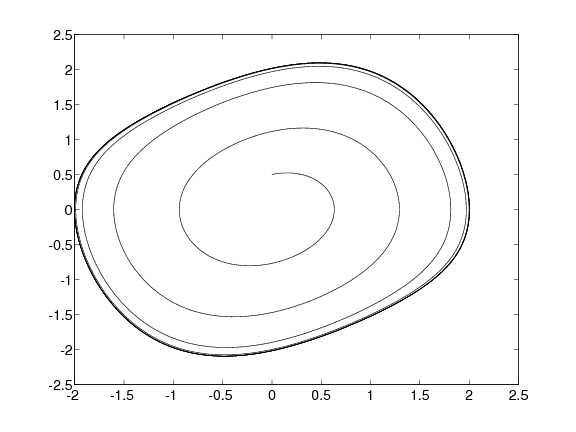
\epsfig{file={../fig/pol03i}}}   
 \caption{$\epsilon=0.3$, initial conditions inside the attractor.}
 \label{figpol03i}
\end{figure}
\begin{figure}[htb]
 \centerline{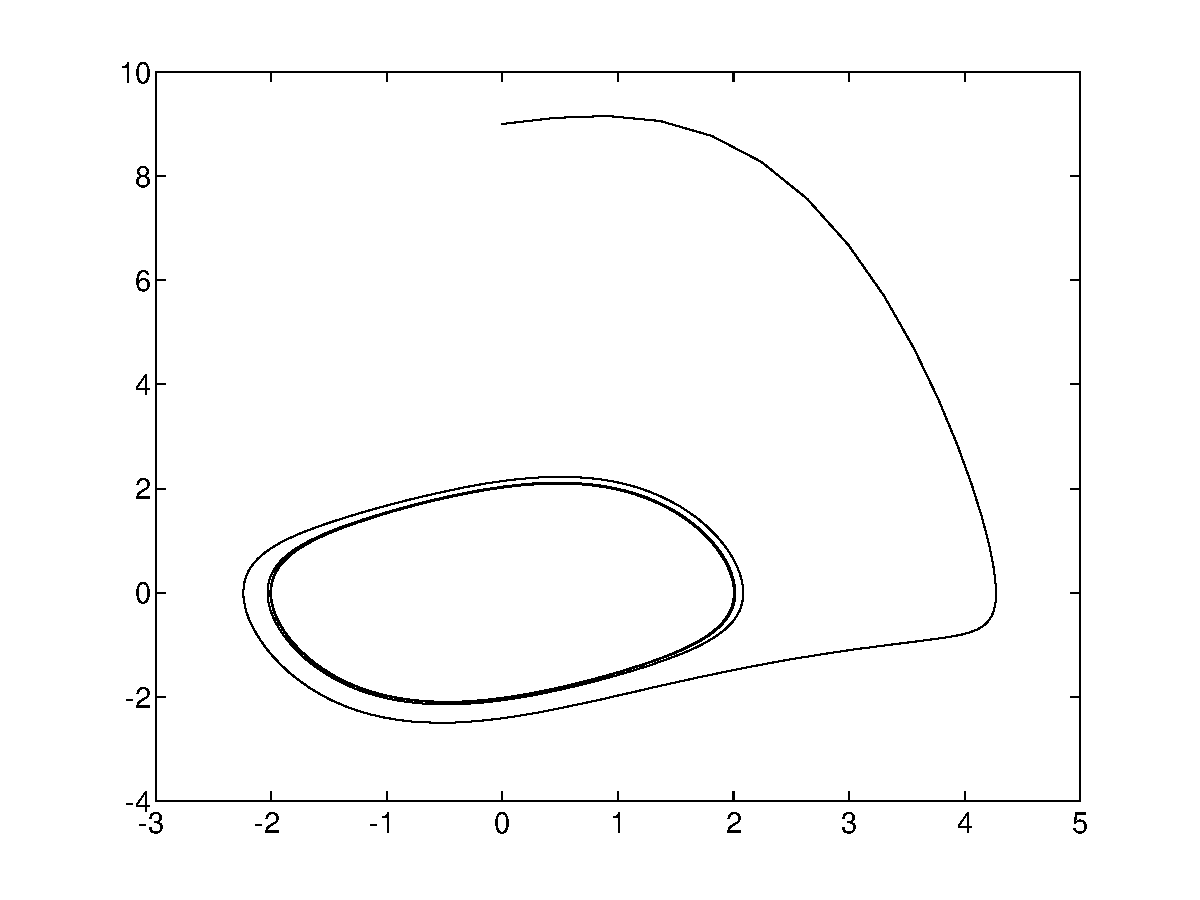
\epsfig{file={../fig/pol03e}}}   
 \caption{$\epsilon=0.3$, initial conditions out of the attractor.}
 \label{figpol03e}
\end{figure}
%
\end{exmp}
\begin{exmp}
Let us consider the reaction diffusion system:
\begin{equation}
\frac{\partial u}{\partial t}=\gamma(a-bu+\frac{u^2}{\nu})+\nabla^2u
\end{equation}
\begin{equation}
\frac{\partial v}{\partial t}=\gamma(u^2-v)+d\nabla^2v
\end{equation}
Figure \ref{figreacd} 
shows results of integration of this system using Euler method (space
treatment is achieved using simple finite differences, periodic boundary
conditions are used). The lattice has
$100 \times 50$ sites.
%
%
\begin{figure}
\begin{tabular}[t]{ccc}

\epsffile{../fig/reacdt1ga5e_04ite2}
\epsffile{../fig/reacdt1ga5e_04ite4}

\epsffile{../fig/reacdt1ga5e_04ite6}
\epsffile{../fig/reacdt1ga5e_04ite8}

\epsffile{../fig/reacdt1ga5e_04ite10}
\epsffile{../fig/reacdt1ga5e_04ite12}

\epsffile{../fig/reacdt1ga5e_04ite14}
\epsffile{../fig/reacdt1ga5e_04ite16}

\epsffile{../fig/reacdt1ga5e_04ite18}
\epsffile{../fig/reacdt1ga5e_04ite20}
\end{tabular} 
\caption{Simulation of reaction diffusion system on a lattice of $100 \times
  50$ sites. A site in black corresponds to a value of $u$ greater than
  $(u_{max}-u_{min})/2$. When time evolves, structures that can model blots on
  some animals skin.}
\label{figreacd}
\end{figure}
Numerical value of parameters were $\gamma=5$, $a=0.5$, $b=2$, $D=10$,
$dt=0.01$. Initial conditions were random, more precisely $u(i,j)=0.25+0.001*rand(i,j)$ and $v(i,j)=0.6+0.001*rand'(i,j)$
where $rand(i,j)$ and $rand'(i,j)$ are random numbers between $0$ and
$1$. Such systems allow to describe spatio temporal systems where two
quantities $u$ and $v$ play a different role: the first is activator of a
change in characteristic of the site , the
second is inhibitor. They can be used to model evolution of forest fires or
blots on the skin of certain animals.
\end{exmp}
\begin{exmp}
Nonlinear Klein-Gordon equation
\begin{equation}
u_{xx}-u_{tt}=F(u)
\end{equation}
where $F$ is (Sine-Gordon equation)
\begin{equation}
F(u)=\sin u
\end{equation}
or (phi four)
\begin{equation}
F(u)=-u+u^3
\end{equation}
can be integrated using a leap-frog scheme\cite{ma:equad:Dodd82} :
\begin{equation}
u_{t+1,k} = -u_{t-1,k}+u_{t,k+1}+ u_{t,k-1}-
h^2F[\frac{1}{2}(u_{t,k+1}+u_{t,k-1})] 
\end{equation}
\end{exmp}

\subsection{Runge-Kutta method}
%%%%%%%%%%%%%%%%%%%%%%
Runge-Kutta formula \index{Runge-Kutta} at fourth order gives $u_{i+1}$ as a
function of $y_i$: 
\begin{equation}
u_{i+1}=u_i+\frac{\Delta
t}{6}[f(u_i,t_i)+2f(uu_{i+\frac{1}{2}},t_{i+\frac{1}{2}})+
2f(uuu_{i+\frac{1}{2}},t_{i+\frac{1}{2}})+ f(uu_{i+1},t_{i+1})]
\end{equation}
where
\begin{equation}
uu_{i+\frac{1}{2}}=u_i+\frac{\Delta t}{2}f(u_i,t_i)
\end{equation}
\begin{equation}
uuu_{i+\frac{1}{2}}=u_i+\frac{\Delta t}{2}f(uu_{i+\frac{1}{2}},t_{i+\frac{1}{2}})
\end{equation}
\begin{equation}
uu_{i+1}=u_i+{\Delta t}f(uuu_{i+\frac{1}{2}},t_{i+\frac{1}{2}})
\end{equation}

\subsection{Adams method (multiple steps)}
%%%%%%%%%%%%%%%%%%%
Problem:

Find $u(t)$ solution of:
\begin{equation}
\frac{d u}{dt}=F(u)
\end{equation}
with
\begin{equation}
u(0)=u_0
\end{equation}
can be solved by 
open Adams\index{Adams formula} method order two:
\begin{equation}
u_{i+1}=y_i+\frac{\Delta t}{2}(3F_i-F_{i-1})
\end{equation}
or open Adams method order three:
\begin{equation}
u_{i+1}=y_i+\frac{\Delta t}{12}(23F_i-16F_{i-1}+5F_{i-2})
\end{equation}
Open Adams method are multisteps: they can not initiate an integration
process. Examples of closed Adams method, are at order two:
\begin{equation}
u_{i+1}=y_i+\frac{\Delta t}{2}(F_{i+1}+F_{i})
\end{equation}
and order three:
\begin{equation}
u_{i+1}=y_i+\frac{\Delta t}{12}(5F_{i+1}-8F_{i}-F_{i-1})
\end{equation}
Closed Adams methods are also multisteps. They are more accurate but are
implicit: they imply the solving of equations systems at each time
step. Predictor--corrector method provides a practical way to use closed Adams
formulas. 
\subsection{Predictor--corrector method}
%%%%%%%%%%%%%%%%%%%%%%%%%%%%%
Predictor--corrector methods\index{predictor-corrector} 
are powerful methods very useful in the case where right--hand side is
complex. An first estimation $\tilde u_{i+1}$ is done (predictor) using open
Adams formula, for instance open Adams formula order three:
\begin{equation}
\tilde u_{i+1}=u_i+\frac{\Delta t}{12}[23F(u_i)-16F(u_{i-1})+5F(u_{i-2})]
\end{equation}
Then, $u_{i+1}$ is re-evaluated using closed Adams formula where $\tilde
u_{i+1}$ computed previously is used to avoid implicity:
\begin{equation}
u_{i+1}=y_i+\frac{\Delta t}{12}[5F(\tilde u_{i+1})-8F(u_{i})-F(u_{i-1})]
\end{equation}
\begin{rem}
Evaluation of $F$ in the second step is stabilizing. Problem
\begin{equation}
\frac{du}{dt}=Lu+N(u)
\end{equation}
where $L$ is a linear operator and $N$ a nonlinear operator will be
advantageously integrated using following predictor--corrector scheme:
\begin{equation}
\tilde u_{i+1}=\exp(L.\Delta t)u_i+\Delta t N(u_i)
\end{equation}
\begin{equation}
u_{i+1}=\exp(L.\Delta t)u_i+\Delta t N(\frac{\tilde u_{i+1}+u_i}{2})
\end{equation}
\end{rem}

\subsection{Symplectic transformation case}
%%%%%%%%%%%%%%%%%%%%%%%%%%%%%%%%%%%%%
Consider\index{symplectic} the following particular case of
evolution problem:  
\begin{prob}
Find solution $[q(t),p(t)]$
\begin{equation}
\frac{dq}{dt}=f(q,p)
\end{equation}
\begin{equation}
\frac{dp}{dt}=g(q,p)
\end{equation}
where $[q(t=0),p(t=0)]$ is known (Cauchy problem) and where functions $f$ and
$g$ come from a hamiltonian $H(q,p)$:
\begin{equation}
f=\frac{\partial H}{\partial p}
\end{equation}
\begin{equation}
g=-\frac{\partial H}{\partial q}\\
\end{equation}
\end{prob}
Dynamics in this case preserves volume element $dq.dp$. Let us define
symplectic \index{symplectic}transformation:
\begin{defn}
Transformation $T$ defined by:
\begin{eqnarray}
q_{n+1}&=&f(q_n,p_n)\\
p_{n+1}&=&g(q_n,p_n)
\end{eqnarray}
is symplectic if its Jacobian has a determinant equal to one.
\end{defn}
\begin{rem}
Euler method adapted to case:
\begin{equation}
\frac{dq}{dt}=V(p)\label{eqsymple1}
\end{equation}
\begin{equation}\label{eqsymple2}
\frac{dp}{dt}=F(q)
\end{equation}
consists in integrating using the following scheme:
\begin{eqnarray}
q_{n+1}&=&q_n+V(p_n)\delta t\\
p_{n+1}&=&p_n+F(q_n)\delta t
\end{eqnarray}
and is not symplectic as it can be easily checked.
\end{rem}
Let us giev some examples of symplectic integrating schemes for system
of equation \ref{eqsymple1} and \ref{eqsymple2}.
\begin{exmp}
Verlet method:
\begin{eqnarray}
q_{n+1}&=&q_n+V(p_n)\delta t\\
p_{n+1}&=&p_n+F(q_{n+1})\delta t
\end{eqnarray}
is symplectic (order 1).
\end{exmp}
\begin{exmp}
Staggered leap--frog scheme
\begin{eqnarray}
\frac{1}{\delta t}(p_{n+1}-p_{n})&=&F(q_{n+\frac{1}{2}})\\
\frac{1}{\delta t}(q_{n+1+\frac{1}{2}}-q_{n+\frac{1}{2}})&=&V(P_{n+1})
\end{eqnarray}
is symplectic (order 2).
\end{exmp}
Figures \ref{codefigure1}, \ref{codefigure2}, and \ref{codefigure3} represent
trajectories computed by three methods: Euler, Verlet, and staggered leap--frog
method for (linear) system describing harmonic oscillator:
\begin{equation}
\left\{ \begin{array}{lcr}
\dot x&=&-y\\
\dot y&=&x
\end{array}\right.
\end{equation}
\begin{figure}[tbh]
\centerline{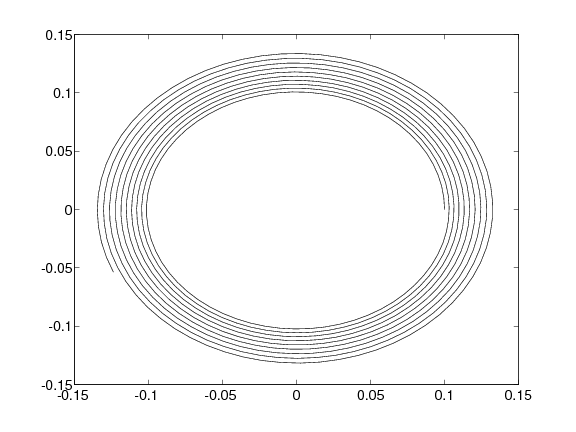
\epsfig{file={../fig/EulerOscillo001}}}
\caption{\it Euler method with time-step $h=0.01$ for harmonic oscillator.}
\label{codefigure1}
\end{figure}
%
\begin{figure}[tbh]
\centerline{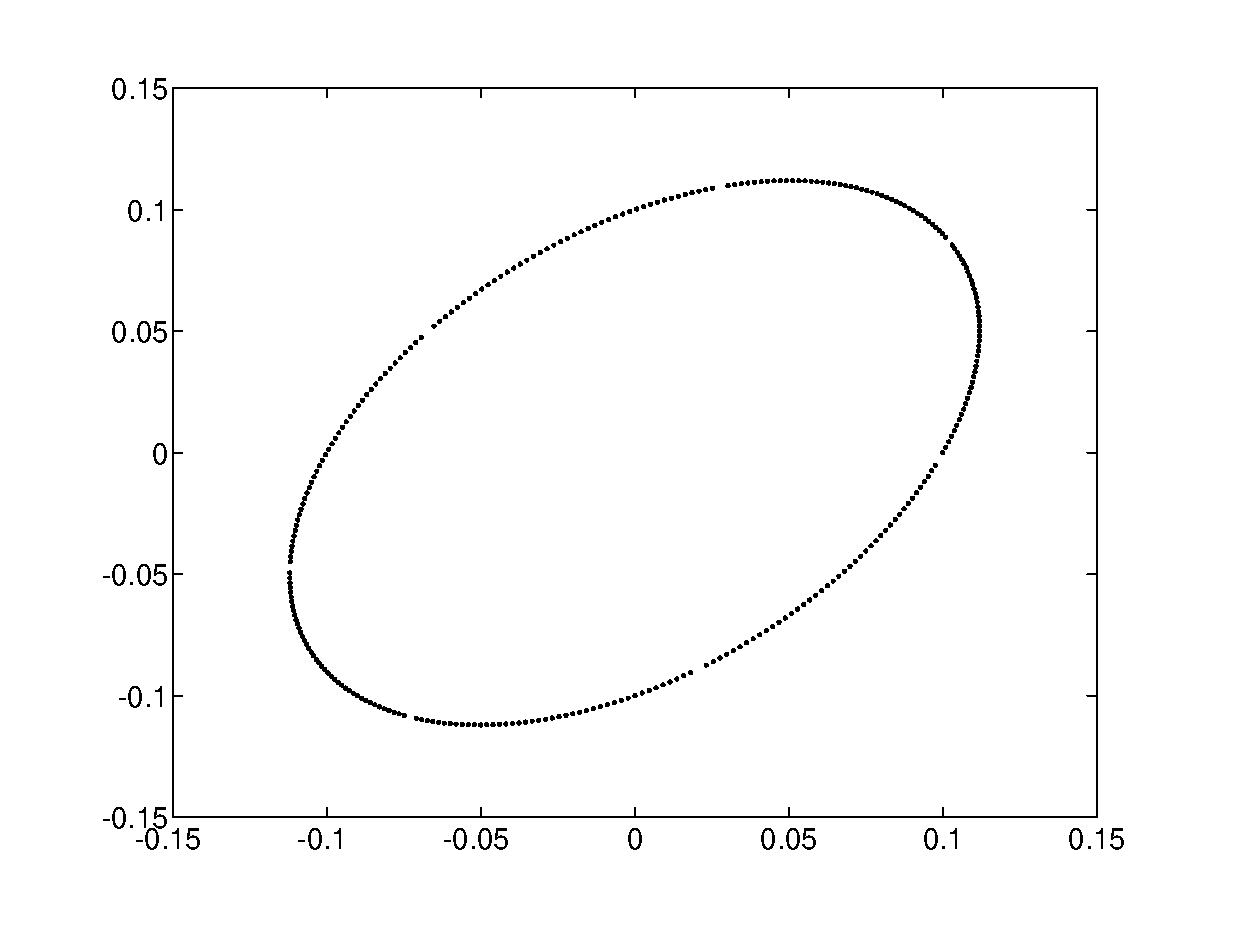
\epsfig{file={../fig/VerletOscillo1}}}   
\caption{\it Verlet method with time step $h=0.9$ for harmonic
  oscillator. Despite a larger time-step than time step used to plot previous
  figure, energy is well conserved.}
\label{codefigure2}
\end{figure}
%
\begin{figure}[tbh]
\centerline{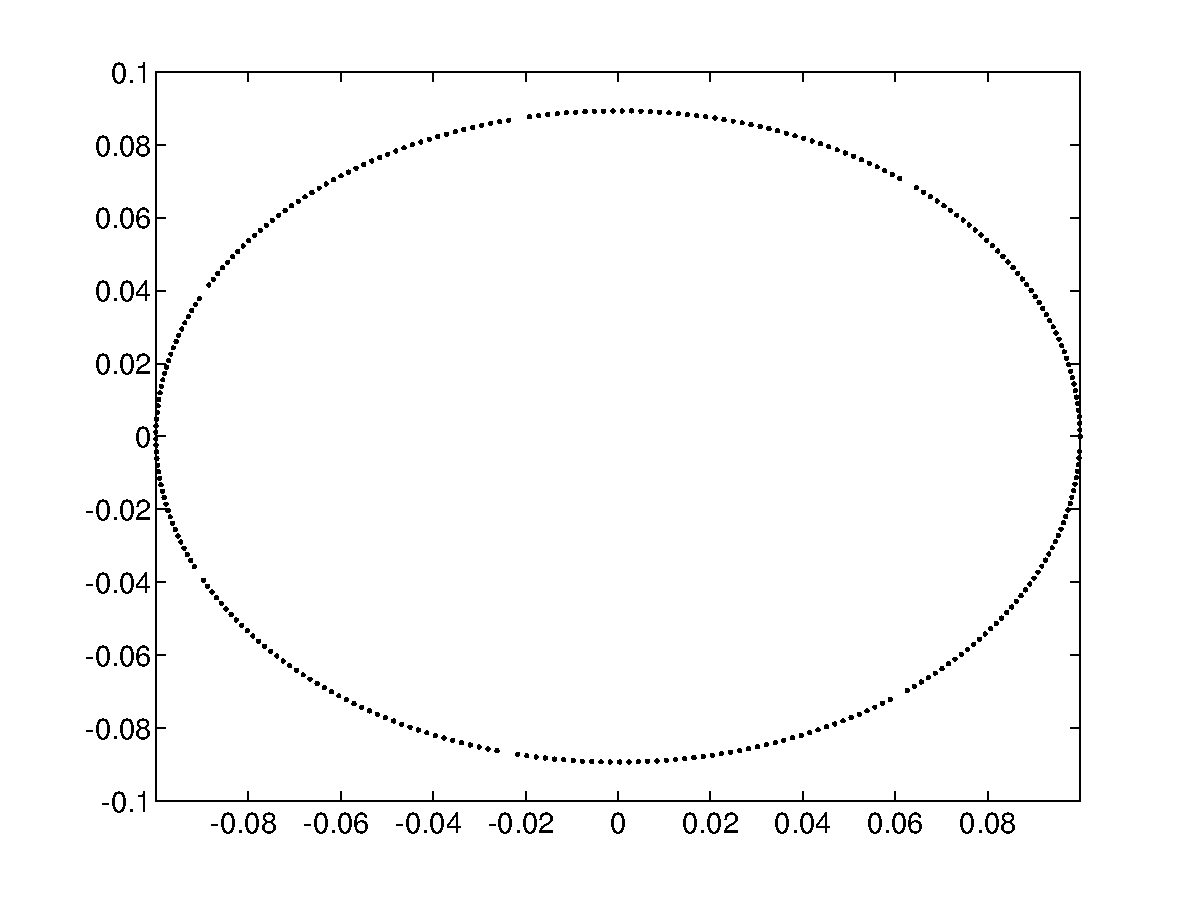
\epsfig{file={../fig/VerletRecOscillo09}}}   
\caption{\it Staggered leap--frog method: energy is still well conserved, but
  space phase is less deformed than in previous case.}
\label{codefigure3}
\end{figure}
%


\section{Particular trajectories and geometry in space phase}
%%%%%%%%%%%%%%%%%%%%%%%


\subsection{Fixed points and Hartman theorem}
%%%%%%%%%%%%%%%%%%%%%%%%%
Consider the following initial value problem:
\begin{equation}\label{eqnl}
\dot x=f(x), x\in R^n
\end{equation}
with $x(0)=0$.
It defines a flow: $\phi_t:R^n\rightarrow R^n$ defined by
$\phi_t(x_0)=x(t,x_0)$.



By Linearization around a fixed point such that $f(\bar x)=0$:



\begin{equation}\label{eql}
\dot \xi=Df(\bar x)\xi, \xi\in R^n
\end{equation}

The linearized flow obeys:
\begin{equation}
D\Phi_t(\bar x)\xi=e^{tDf(\bar x)}\xi
\end{equation}



It is natural to ask the following question:
What can we say about the solutions of \ref{eqnl} based on our
knowledge of \ref{eql}?

\begin{thm}
If $Df(\bar x)$ has no zero or purely imaginary eigenvalues, then
there is a homeomorphism $h$ defined on some neighborhood $U$ of $\bar
x$ in $R^n$ locally taking orbits of the nonlinear flow $\phi_t$ to
those of the linear flow $e^{tDf(\bar x)}$. The homeomorphism
preserves the sense of orbits and can be chosen to preserve
parametrization by time.
\end{thm}

When $Df(\bar x)$ has no eigen values with zero real part, $\bar x$ is
called a {\bf hyperbolic} or nondegenerate fixed point and the asymptotic
behaviour near it is determined by the linearization.

In the degenerate case, stability cannot be determined by
linearization.

Consider for example:

\begin{equation}
\left( \begin{array}{c}
\dot x_1\cr \dot x_2
\end{array} \right)
=
\left( \begin{array}{cc}
0&1\cr 
1&0
\end{array} \right)
\left( \begin{array}{c}
x_1\cr x_2
\end{array} \right)
-
\epsilon
\left( \begin{array}{c}
0\cr
x_1^2x_2
\end{array} \right)
\end{equation}

Eigenvalues of the linear part are $\pm i$.
If $\epsilon>0$: a spiral sink, if  $\epsilon<0$: a repelling source,
if $\epsilon=0$ a center (hamiltonian system).

\subsection{Stable and unstable manifolds}
%%%%%%%%%%%%%%%%%%%%%%%%%%%%%%%%%%%%%%%%%

\begin{defn}
The local stable and unstable manifolds $W^s_{loc}$ and $W^u_{loc}$ of
a fixed point $x^*$ are
\begin{equation}
W^s_{loc}=\{x\in U \| \phi_t(x)\rightarrow x^* \mbox{  as  } t\rightarrow
+\infty, \mbox{ and } \phi_t(x)\in U \mbox{  for all  } t\geq 0\}
\end{equation}
\begin{equation}
W^u_{loc}=\{x\in U \| \phi_t(x)\rightarrow x^* \mbox{  as  } t\rightarrow
-\infty, \mbox{ and } \phi_t(x)\in U \mbox{  for all  } t\leq 0\}
\end{equation}
where $U$ is a neighborhood of the fixed point $X^*$.
\end{defn}

\begin{thm}
(Stable manifold theorem for a fixed point). Let $x^*$ be a hyperbolic
fixed point. There exist local stable and unstable manifold
$W^s_{loc}$ and $W^u_{loc}$ of the same dimesnion $n_s$ and $n_u$ as
those of the eigenspaces $E^s$, and $E^u$ of the linearized system,
and tangent to $E^u$ and $E^s$ at $x^*$. $W^s_{loc}$ and $W^u_{loc}$
are as smooth as the function $f$.
\end{thm}

An algorithm to get unstable and stable manifolds is given in
\cite{ma:compu:Parker89}.
It basically consists in finding an point $x_\alpha$ sufficiently
close to the fixed 
point $x^*$, belonging to an unstable linear eigenvector space:
\begin{equation}\label{eqalphchoose}
x_\alpha=x^*+\alpha e_u.
\end{equation}
For continuous time system, to draw the unstable manifold, one has
just to integrate forward in time from $x_\alpha$.
For discrete time system, one has to integrate forward in time the
dynamics for points in the segement $\mathrel{]}\Phi^{-1}(x_\alpha),x_\alpha\mathrel{]}$
where $Phi$ is the application.

The number $\alpha$ in equation \ref{eqalphchoose} has to be small
enough for the linear approximation to be accurate. Typically, to
choose $\alpha$ one compares the distant between the images of
$x_\alpha$ given by the linearized dynamics and the exact dynamics. If
it is too lage, then $\alpha$ is divided by 2. The process is iterated
untill an acceptable accuracy is reached.



\subsection{Periodic orbits}
%%%%%%%%%%%%%%%%%%%%%%%%%%%%

It is well known \cite{ma:equad:Guckenheimer83} that there exist periodic 
(unstable) orbits in a chaotic system. 
We will first detect some of them.
A periodic orbit in the 3-D phase space corresponds to a
fixed point of the Poincar\'e map.

The method we choosed to  locate periodic orbits is 
``the Poincare map'' method\cite{ma:compu:Parker89}.
It uses the fact that periodic orbits correspond to fixed
points of Poincare maps.
We chose the plane $U=0$ as one sided Poincare section.
(The 'side' of the section is here defined by $U$ becoming 
positive)

Let us recall the main steps in locating periodic orbits
by using the Poincare map method :
we apply
the Newton-Raphson algorithm to the application
$H(X)=P(X)-X$ where $P(X)$ is the Poincare map
associated to our system which can be written as :
\begin{equation}
\frac{dX}{dt}=F_\epsilon(X)
\end{equation}
\begin{equation}
X(0)=X_0
\end{equation}

where $\epsilon$ denotes the set of the control
parameters.
Namely, the Newton-Raphson algorithm is here :
\begin{equation}\label{eqnewton}
X^{k+1}=X^k-(DP_{X^k}-I)^{-1}(P(X^k)-X^k)
\end{equation}
where $DP_{X^k}$ is the Jacobian of the Poincare map
$P(X)$ evaluated in $X^k$.


The jacobian of poincare map $DP$ needed in the scheme
of equation \ref{eqnewton} is computed via 
the integration of
the dynamical system:
\begin{equation}
\frac{dX}{dt}=F_\epsilon(X)
\end{equation}
\begin{equation}
X(0)=X_0
\end{equation}
\begin{equation}
\frac{d\Phi^t}{dt}=DF_{X,\epsilon}.\Phi^t
\end{equation}
\begin{equation}
\Phi^0=Id
\end{equation}
where $DF_{X,\epsilon}$ is the Jacobian of $F_\epsilon$ in 
$X$, and $X_0$ is a Point of the Poincare section.
We chose a Runge--Kutta scheme, fourth order
\cite{ma:compu:Parker89,ma:compu:Press92} for the
time integration of the whole previous system.
The time step was $0.003$.

We have the relation :
\begin{equation}
DP_X=\left( I-\frac{F(P(X)).h^+}{F(P(X))^+.h}\right)\Phi^T
\end{equation}
where $T$ is the time needed at which the trajectory
crosses le Poincare section again.

\begin{rem}
Note that a good test for the accuracy of the integration 
is to check that on a periodic orbit, there is one eigenvalue of
$\Phi^T$ which is one.
\end{rem}

\section{Use of change of variables}
\subsection{Normal forms}
%%%%%%%%%%%%%%%%%%%%%%
As written in \cite{ma:equad:Arnold83} it is very powerfull not to
solve differential equations but to tranform them into a simpler
differential equation.
\cite{ma:equad:Arnold83,ma:equad:Guckenheimer83,ma:equad:Berry78}
Let the system:
\begin{equation}
\dot x=F(x)
\end{equation}
and $x^*$ a fixed point of the system: $F(x^*)=0$. Without lack of
generality, we can asssume $x^*=0$.
Assume that application $F$ can be develloped around $0$:
\begin{equation}
F(x)=Ax+\dots
\end{equation}
where the dots represent polynomial terms in $x$ of degree $\geq 2$.
There exists the following lema:
\begin{thm}\label{lemplo}
Let $h$ be a vectorial polynom of order $r\geq 2$ and
$h(0)=h^\prime(0)=0$. The change of variable $x=y+h(y)$ transforms the
differential equation $\dot y=Ay$ into the equation:
\begin{equation}
\dot x=Ax+v(x)+\dots
\end{equation}
where $v(x)=\frac{\partial h}{\partial x}Ax-Ah(x)$ and where the dots
represent terms of order $>r$.
\end{thm}
\begin{equation}
\dot x=(I+\partial_y h)A(x-h(x))+\dots= Ax+[\frac{\partial h}{\partial
x}Ax-Ah(x)] 
\end{equation}
Note that $\frac{\partial h}{\partial x}Ax-Ah(x)$ is the Poisson
crochet between $Ax$ and $h(x)$.
We note $L_Ah=\frac{\partial h}{\partial x}Ax-Ah(x)$ and we call the
following equation:
\begin{equation}
L_Ah=v
\end{equation}
the homological equation associated to the linear operator $A$.

We are now interested in the reverse step of theorem \ref{lemplo}: We
have a nonlinear system and want to find a change of variable that
transforms it into a linear system.
For this we need to solve the homological equation, {\it i.e.} to
express $h$ as a function of $v$ associated to the dynamics.

Let us call
$e_i$, $i\in (1,\dots,n)$ the basis of eigenvectors of $A$,
$\lambda_i$ the associated 
eigenvalues, and $x_i$ the coordinates of the system is this basis.
Let us write $v=v_r+\dots$ where $v_r$ contains the monoms of degree
$r$, that is the terms $x^{m}=x_1^{m_1}\dots x_n^{m_n}$, $m$ being
a set of positive integers $(m_1,\dots,m_n)$ such that $\sum m_i=r$. 
It can be easily checked (see \cite{ma:equad:Arnold83}) that the monoms
$x^me_s$ are eigenvectors of $L_A$ with eigenvalue 
$(m,\lambda)-\lambda_s$ where
$(m,\lambda)=m_1\lambda_1+\dots+m_n\lambda_n$:
\begin{equation}
L_Ax^me_s=[(m,\lambda)-\lambda_s]x^me_s.
\end{equation}
One can thus invert the homological equation to get a change of
variable $h$ that eliminate the nonom considered. 
Note however, that one needs $(m,\lambda)-\lambda_s\neq 0$ to invert
previous equation.
If there exists a $m=(m_1,\dots,m_n)$ with $m_i\geq 0$ and $\sum
m_i=r\geq 2$ such that 
$(m,\lambda)-\lambda_s=0$, then the set of eigenvalues $\lambda$ is
called resonnant.
If the set of eigenvalues is resonant, since there exist such $m$,
then monoms $x^me_s$ can not be eliminated by a change of variable.
This leads to the {\bf normal form theory} \cite{ma:equad:Arnold83}.

\subsection{KAM theorem}
%%%%%%%%%%%%%%%%%%%

An hamiltonian system is called {\bf integrable} if there exist
coordinates $(I,\phi)$ such that the Hamiltonian
doesn't depend on the $\phi$.
\begin{equation}\label{eqbasimom}
\frac{dI_i}{dt}=-\frac{\partial H}{\partial \phi_i}=0
\end{equation}
\begin{equation}
\frac{d\phi_i}{dt}=-\frac{\partial H}{\partial I_i}
\end{equation}
Variables $I$ are called action and variables $\phi$ are called
angles.
Integration of equation \ref{eqbasimom} is thus immediate and leads to:
\begin{equation}
I=I_0
\end{equation}
and $\phi_i=\omega_i(I)t+\phi_i^0$ where $\omega_i(I)=-\frac{\partial
H}{\partial I_i}$ and $\phi_i^0$ are the initial conditions.


Let an integrable system described by an Hamiltonian $H_0(I)$ in the
space phase of the action-angle variables $(I,\phi)$.
Let us perturb this system with a perturbation $\epsilon H_1(I,\phi)$.

\begin{equation}
H(I,\phi)=H_0(I)+\epsilon H_1(I,\phi)
\end{equation}
where $H_1$ is periodic in $\phi$.

If tori exist in this new system, there must exist new action-angle
variable $(I^\prime,\phi^\prime)$ such that:
\begin{equation}\label{eqdefHip}
H(I,\phi)=H^\prime(I^\prime)
\end{equation}

{\bf Change of variables} in Hamiltonian system can be
characterized\cite{ph:mecac:Goldstein80} by a
function $S(\phi,I^\prime)$ called {\bf generating function} that
satisfies: 
\begin{equation}
I=\frac{\partial S}{\partial \phi}
\end{equation}
\begin{equation}
\phi^\prime=\frac{\partial S}{\partial I^\prime}
\end{equation}
If $S$ admits an expension in powers of $\epsilon$ it must be:
\begin{equation}
S=\phi I^\prime+\epsilon S_1(\phi,I^\prime)+\dots
\end{equation}
Equation \ref{eqdefHip} thus becomes:
\begin{equation}\label{equatfondKAM}
H_0(I^\prime)+\epsilon\partial_{I^\prime_i}H(I^\prime)\partial_{\phi_i}
+H_1(I^\prime,\phi)=H^\prime(I^\prime)
\end{equation}
Calling $\omega_0$ the frequencies of the unperturbed Hamiltionan
$H_0$:
\begin{equation}
\omega_{0,i}(I^\prime)=\partial_iH_0(I^\prime)
\end{equation}

Because $H_1$ and $S_1$ are periodic in $\phi$, they can be decomposed
in Fourier:

\begin{equation}
H_1(I,\phi)=\sum_m H_{1,m}(I)e^{im\phi}
\end{equation}

\begin{equation}
S_1(I,\phi)=\sum_{m\neq 0} S_{1,m}(I)e^{im\phi}
\end{equation}

Projecting on the Fourier basis equation \ref{equatfondKAM} one gets
the expression of the new Hamiltonian:
\begin{equation}
H^\prime(I^\prime)=H_0^\prime(I^\prime)+\epsilon H^\prime(I^\prime)
\end{equation}
and the relations:
\begin{equation}
i.m.\omega_0(I^\prime) S_{1,m}(I^\prime)=H_{1,m}(I^\prime)
\end{equation}

Inverting formally previous equation leads to the generating function:
\begin{equation}
S(\phi,I^\prime)=\phi I^\prime+\epsilon i \sum_{m\neq
0}\frac{H_{1,m}(I^\prime)}{m.\omega_0(I^\prime)} 
\end{equation}
The problem of the convergence of the sum and the expansion in
$\epsilon$ has been solved by KAM.
Clearly, if the $\omega_i$ are resonnant (or commensurable), the serie
diverges and the torus is destroyed. 
However for non resonant frequencies, the denominator term can be very
large and the expansion in $\epsilon$ may diverge.
This is the {\bf small denominator
problem}. 

In fact, the KAM theorem states that tori with ``sufficiently
incommensurable'' frequencies\footnote{%%%%%%%%%%%%%%%%%
In the case two dimensional
case  the KAM
theorem proves that the tori that are not destroyed are those with two
frequencies $\omega_{0,1}(I)$ 
and  $\omega_{0,2}(I)$ whose ratio $\omega_{0,1}(I)/\omega_{0,2}(I)$
is sufficiently irrational for the following relation to hold:
\begin{equation}
\left|\frac{\omega_{0,1}}{\omega_{0,2}}-\frac{r}{s}\right|>
\frac{K(\epsilon)}{s^{2.5}}\mbox{ , for all integers } r\mbox{ and } s,
\end{equation}
where $K$ is a number that tends to zero with the $\epsilon$.

} 
are not destroyed: The serie converges\footnote{%%%%%%%%% 
To prove the convergence, KAM use an accelerated convergence method
that, to calculate the torus at
order $n+1$  uses the torus calculated at order $n$ instead of the
torus at order zero like an classical Taylor expansion. See
\cite{ma:equad:Berry78} for a good analogy with the relative speed of the Taylor
expansion and the Newton's method to calculate zeros of functions.
}.%%%%%%%%%%%%%%%%%%%%%%%



\section{Abstract}
%%%%%%%%%%%%%%%%%%%%
We have presented in this chapter three great classes of problems encountered
in the study and modelling of physical systems:
Boundary problems, evolution problems and spectral problems that can arise
from the solving of linear evolution problems.
We have considered integral and variational methods for the treatment of
boundary problems. Spectral method have been introduced for solving linear
evolution problems. 
Various aspects of perturbative approach have been presented as well as
numerical scheme for time integration useful for nonlinear evolution
problems. 

\section{Exercises}
%%%%%%%%%%%%%%%%%

\begin{exo}
Show directly ({\it i.e.}, 
using Green formula that in the case of the sliding string, the average
applied force have to be zero for the system to have a solution.
\end{exo}

\begin{exo}
Show by recurrence the result given without proof at remark \ref{remmatrindep}.
\end{exo}

\begin{exo}
Find, using Green's method, the solution of problem $P(f,\phi,\psi)$
(Problem \ref{probpfppgreen})
(non homogenous problem) in the case where $\mbox{Ker}(L^*)$ is non zero.
\end{exo}


\begin{exo}\label{exoentr}
Find, using Lagrange multipliers method, the distribution of $P_l$
solution of the 
following maximization problem:
Maximize the function $S$ (the entropy in statistical physics) 
\begin{equation}
S=-k_B\sum_{(l)}P_l\ln P_l
\end{equation}
with $n+1$ constraints: 
\begin{equation}
R_0=\sum P_l-1=0
\end{equation}
\begin{equation}
R_i=\sum X^i_lP_l-\bar X^i=0, i=1,\dots,n
\end{equation}
\end{exo}


\begin{exo}\label{exospectramatrice}
In the present chapter we have seen the spectral method to solve PDE.
Recall the spectral method used to solve the following ODE problem:
Find $X$ such that
\begin{equation}\label{eqevol}
\frac{dX}{dt}=L X
\end{equation}
with
\begin{equation}
X(0)=X_0
\end{equation}
where $L$ is a $n
\times n$ matrix and $X$ is a vector of dimension $n$.
Apply this method to solve the evolution problem describing the dynamics of
two coupled oscillators:
\begin{equation}
\ddot x_1=-\frac{k}{2m}x_1+\frac{k}{m}x_2
\end{equation}
\begin{equation}
\ddot x_2=+\frac{k}{m}x_1-\frac{k}{2m}x_2
\end{equation}
where $x_1$ and $x_2$ are distances to equilibrium.
\end{exo}


\begin{exo}\label{exocordespec}
Solve using spectral method the evolution problem of a string between
two walls. The evolution equation of transversal vibrations is:
\begin{equation}
\frac{\partial^{2}}{\partial
x^{2}}u(x,t)=\frac{1}{c^2}\frac{\partial^{2}}{\partial t^{2}}u(x,t)
\end{equation}
Consider two boundary conditions:
\begin{enumerate}
\item 
\begin{equation}
u(0,t)=0,
\end{equation}
\begin{equation}
u(l,t)=0
\end{equation}
Those first boundary conditions correspond to a string clamped between
two walls.
\item 
\begin{equation}
\frac{\partial}{\partial x}u(0,t)=0, 
\end{equation}
\begin{equation}
\frac{\partial}{\partial x}u(l,t)=0
\end{equation}
Those second boundary conditions correspond to a sliding string. 
\end{enumerate}
Initial conditions are given by:
\begin{equation}
u(x,0)=u^1(x),\:\frac{\partial}{\partial t}u(x,0)=u^2(x)
\end{equation}
\end{exo}


\begin{exo}
Generalize the perturbative method presented at section \ref{chapmethspec}
for the spectral analysis of an operator going from a space $H_{1}$ to a space
$H_{2}$ different from $H_1$. 
Such a spectral decomposition is called singular value decomposition in
numerical analysis books, Karhumen Lo\`eve decomposition in statistics and 
biorthogonal decomposition in nonlinear dynamics.
\end{exo}


\begin{exo}\label{exopoincalin}
Consider the nonlinear oscillator whose evolution is described by equation:
\begin{equation}
\left[\omega^2\partial_{\tau}\partial_{\tau}-
  \partial_{x}\partial_{x}\right]u-f(u)=0 
\end{equation}
Find solution $u$ of previous equation by using Poincar\'e-Lindstedt method.
\end{exo}


\chapter{N body problem and matter description}\label{chapnbodpmatter}
%%%%%%%%%%%%%%%%%%%%%%%%%%%%%%%%%%%%%%
\section{Introduction}
%%%%%%%%%%%%%%%%%%%%%%
As noted in the introduction to this book, $N$ body
problem\cite{ph:physt:March95,ph:physt:Mattuck92}  is the
fundamental 
problem that spanned modern physics, sustaining reductionnist approach
of Nature. 
The element considered depend on the scale chosen to describe the matter.
Each field of physics has its favourite N body problem:
\begin{itemize}
\item nuclear physics deals with sets of nucleons.
\item atomic physics deals with interactions between nucleus and nucleons.
\item molecular chemistry, solid state physics, physics
of liquids, gas, plasmas deals with interactions between atoms.
\item classical mechanics and electrodynamics, $N$ body problems can arise
  (planet movement for instance). 
\item en astrophysics one studies interactions between stars, galaxies, and
  clusters of galaxies.
\end{itemize}
Once fundamental elements making matter are identified, the interaction
between systems made of $N$ such fundamental elements should be
described.  Note that the interaction between constituents change with the
lenght scale considered. Nuclear 
physics deals mostly with strong interaction (and weak
interaction). Atomic physics and molecular physics deal 
mostly with electromagnetic interaction. Astrophysics deals with
gravitation and ther other interactions\footnote{Indeed, in the
description of stars for instance, gravitational pressure implies that
fusion reaction are possible and that all atoms are ionized, thus
interacting via electromagnteic interaction}%%%%%%%%%%%%%%%%%%

This chapter is purely descriptive. No equations are presented. The
subatomic systems will not be more treated in the next
chapters. However, the various forms of matter that can be considered
using, as elementary block, atomic nucleus and its electrons will be treated in
the rest of the book. For each form of matter presented here, numerous
references to other parts of the books are proposed. Especially, chapter 
\ref{chapproncorps}, treats of quantum properties of eigenstates of such
systems (the Schr\"odinger evolution equation is solved by the spectral
method). Chapter \ref{chapNcorpsstat} treats of their statistical properties.

\section{Origin of matter}
%%%%%%%%%%%%%%%%%%%%%%%%%%
\index{matter (origin of)}\index{origin of matter}
The problem of the creation of the Universe is an open problem. 
Experimental facts show that Universe is in expansion\footnote{The red-shift
phenomenon was summerized by Hubble in 
1929. The Hubble's law states that the shift in the light received
from a galaxy is proportional to the distance from the observer point
to the galaxy.}
Inverting the time arrow, this leads to a Universe that has explosive
concentration. Gamow, a genial physicist, proposed in 1948 a model
known as, Big Bang model\index{Big Bang model}, for the creation of
the Universe. When it 
was proposed the model didn't receive much attention, but in 1965 two
engineers from AT\&T, Penzias and Wilson\footnote{They received the
physics Nobel price in 1978}%%%%%%%%%%%%%%%%%%%%%%
, trying to improve communication between earth and
a satellite, detected by accident a radiation foreseen by Gamow and his
theory: the 
{\bf 3K cosmic background radiation}\index{cosmic background radiation}.
In 1992, the COBE
satellite (COsmic Background Explorer) recorded the fluctuations in
the radiation (see figure \ref{figcobe}), which should be at the
origin of the galaxy formation as we will see now. 
\begin{figure}[htb]
 \centerline{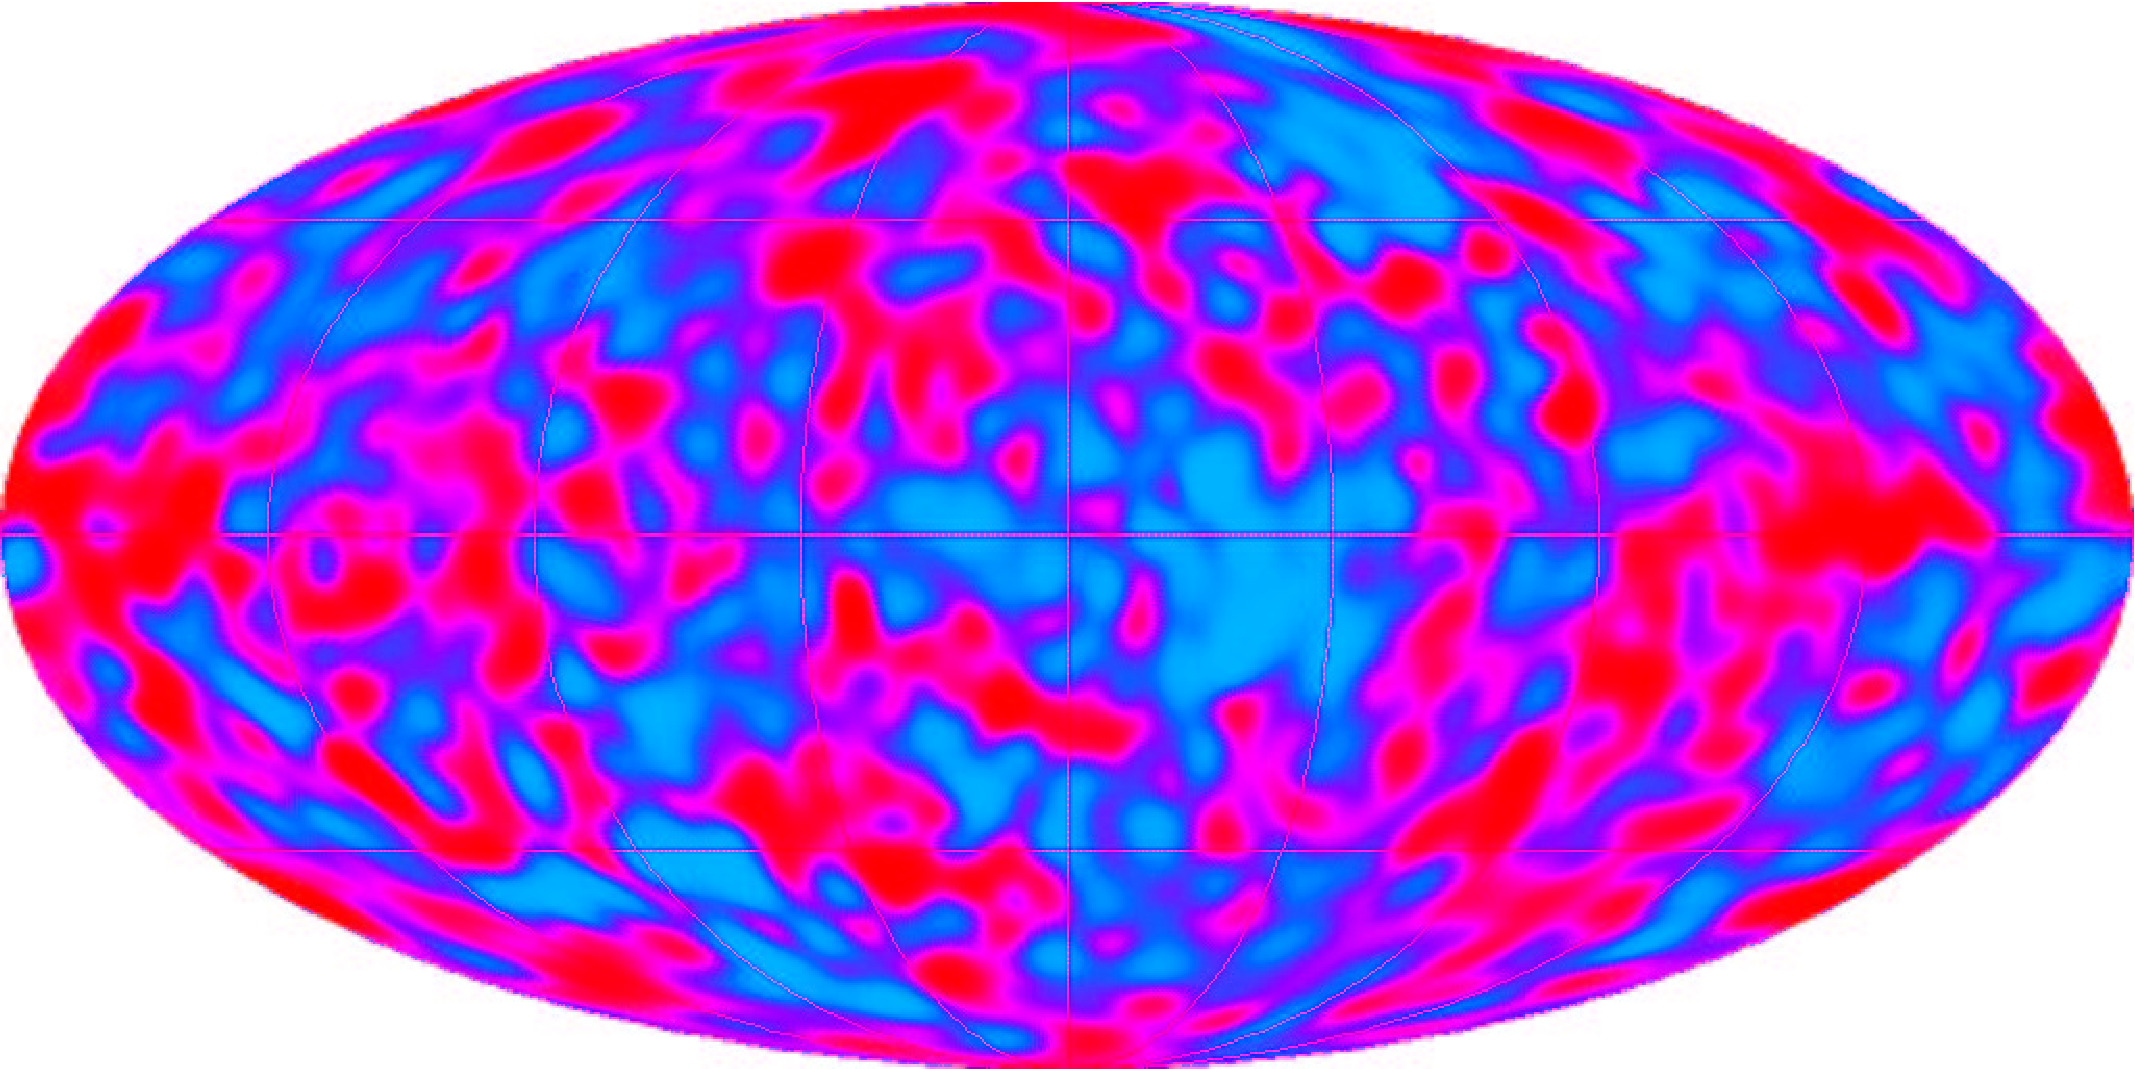
\epsfig{file={../fig/cmbr_DMR_white}}}   
 \caption{Cosmic backgroung radiation as recorded by COBE}
 \label{figcobe}
\end{figure}
The Big Bang model states that the history of the Universe obeys to
the following chronology\footnote{Time origin corresponds to Universe
creation time}: 

\begin{itemize}
\item During the first period (from $t=0$ to $t=10^{-6}$ s), universe
density is huge 
(much greater than the nucleons density)\footnote{Describing waht
componds Universe at during this period is a challenge to
human imagination.} It's behaviour is like a black hole. Quarks may
exist independantly. 
\item The hadronic epoch\footnote{Modern particle accelerators reach
such energies. The cosmology, posterior to $t=10^{-4}$ s is called
``standard'' and is rather well trusted. On the contrary, cosmology
before the hadronic period is much more speculative.},%%%%%%%%%%%%%
(from $t=10^{-6}$, $T=1$GeV (or
$T=10^{13}$K) to $t=10^{-4}$ s, $T=100$ MeV), the black hole
radiation creates hadrons (particle undergoing strong interaction like
proton, neutrons), leptons (particle that undergo weak interaction
like electrons and neutrinos\footnote{Neutrinos are particles without
electric charge and with a very small mass so that on the contrary to
electrons they don't undergo electrostatic interaction.}) and photons.
The temperature is such that strong interaction can express itself by
assembling quarks into hadrons. During this period no quark can be
observe independantly.
\item During the leptonic epoch, (from $t=10^{-4}$ s, $T=100$ MeV to
$t=10$ s, $T=1$MeV) hadrons can no
more be created, but leptons can still be created by photons (reaction
$\gamma \leftrightarrow e^+ + e^-$). The temperature is such that
strong interaction can express itself by assembling  hadrons into
nuclei. Thus indepandant hadrons tend to disappear, and typically the
state is compound by: leptons, photons, nuclei\footnote{%%%%%%%%%%
Note that
heavy nuclei are not created during this period, as it was believed
some years at the beginning of the statement of the Big band
model. Indeed, the helium nucleus is very stable and prevents heavier
nuclei to appear. Heavier nuclei will be created in the stellar phase
by fusion in the kernel of the stars.}.%%%%%%%%%%%%%%%%%%%%%%%%%%%%%%

\item From $t=10$ s, $T=1$MeV to $t=400,000$ years, $T=1$eV (or
$T=3,000$K), density and temperature decrease and Universe enter the photonic
epoch (or radiative epoch). At such temperature, leptons (as
electrons) can no more be created. They thus tend to disappear as
independant particles, reactionning with nuclei to give
atoms (Hydrogen and helium) and molecules\footnote{%%%%
As for the nuclei, not all the atoms and molecules can be
created. Indeed, the only reactive atoms, the hydrogen atom (the
helium atom is not chemically reactive) gives only the H$_2$ molecule
which is very stable.}%%%%%%%%%%%%
 (H$_2$). The
interaction involed here is the electromagnetic interaction (cohesion
of electrons and nuclei is purely electromagnetic). Typically the
state is compound by: photons, atoms, molecules and electrons. The
radiative epoch ends by definition when there are no more free electrons.
Light and matter are thus decoupled. This is the origin of the cosmic
background radiation. Universe becomes ``transparent'' (to
photons). Photons does no more colide with electrons.
\item From $t=400,000$ years, $T=1$eV (or
$T=3,000$K) untill today ($t=1.5 10^{10}$ years, $T=3$K), Universe
enters the stellar epoch. This is now the kingdom of the
gravitation. Because of (unexplained) fluctuations is the gas density,
particles (atoms and molecules) begin to gather under gravitation to
for prostars and stars.
\end{itemize}
Let us now summerize the stellar evolution and see how heavier atoms
can be created within stars.
The stellar\index{star} evolution can be summerized as follows:
\begin{itemize}
\item {\bf Protostar}: As the primordial gas cloud starts to collapse under
gravity, local regions begin to form  protostars, the precursors to
stars. Gravitational energy which is 
released in the contraction begins to heat up the centre of the
protostar.
\item Main sequence star: gravitational energy leads the hydrogen
fusion to be possible. This is a very stable phase.
Then two evolutions are possible:
%%%%%%%%
\item If the mass of the star is less that $1.4$ (the
Chandrasekhar\footnote{The Indian physicist Subrehmanyan Chandrasekhar
received the physics Nobel price in 1983 for his theoretical studies of the
structure and evolution of stars.} 
limit)\index{Chandrasekhar limit} the mass of the
sun, 
\begin{itemize}
\item The main sequence star evolves to a {\bf red giant star}.
\index{red giant star}
The core is now
composed mostly of helium nuclei and electrons, and begins to
collapse, driving up the core temperature, and increasing the rate at
which the remaining hydrogen is consumed. The outer portions of the
star expand and cool.
\item the helium in the core fuses to form carbon
in a violent event know as the {\bf helium flash}\index{helium flash},
lasting as little as only 
a few seconds.  The star gradually blows away its outer atmosphere
into an expanding shell of gas known as a {\bf planetary nebula}
\index{planetary nebula}.
\item The remnant portion is known
as a {\bf white dwarf}\index{white dwarf}. Further contraction is no
more possible since 
the whole star is supported by electron degeneracy. No more fusion
occurs since temperature is not sufficient. This star
progressively cooles and evolves towards a {\bf black dwarf star}.
\end{itemize}
%%%%%%%%%%%%%%%%%%%%%%%%%%%%%%%%%
\item If the mass of the star is greater that $1.4$ the mass of the
sun, 
\begin{itemize}
\item When the core of massive star becomes depleted of hydrogen, the
gravitational collapse is capable of generating sufficient energy that
the core can begin to fuse helium nuclei to form carbon. In this stage
it has expanded to become a red giant, but brighter. It is known as a
{\bf supergiant}\index{supergiant star}. Following depletion of the helium,
the core can 
successively burn carbon, neon, etc, until it finally has a core of
iron, the last element which can be formed by fusion without the input
of energy. 
\item Once the silicon has
been used the iron core then collapses violently, in a fraction of a
second. Eventually neutron degeneracy prevents the core from ultimate
collapse, and the surface rebounds, blowing out as fast as it
collpased down. As the surface collides with the outer portions of the
star an 
explosion occurs and the star is destroyed in a bright flash. The
material blown out from the star is dispersed into space as a
nebula. The remnants of the core becomes 
\begin{itemize}
\item If the mass of the star is less than $3$ sun's mass, star
becomes a {\bf neutron star}\index{neutron star}. The core collapses
further, pressing the 
protons and electrons together to form neutrons, until neutron
degeneracy stablilises it against further collapse. Neutron stars have
been detected because of their strange emission characteristics. From
the Earth, we see then a pulse of light, which gives the neutron star
its other name, a {\bf pulsar}\index{pulsar}. 
\item  If the mass of the star is greater than $3$ sun's mass, star
becomes a {\bf black hole}\index{black hole}. When stars of very large
mass explode in a 
supernova, they leave behind a core which is so massive (greater than
about 3 solar masses) that it cannot be stabilized against
gravitational collapse by an known means, not even neutron
degeneracy. Such a core is detined to collapse indefinitely until it
forms a black hole, and object so dense that nothing can escape its
gravitational pull, ot even light. 
\end{itemize}
\end{itemize}
\end{itemize}
Let us now start the listing of matter forms observed at a super
nuclear scale (sacle larger than the nuclear scale).

\section{Atoms}
%%%%%%%%%%%%%%%%%%%
Atoms are \cite{ph:atomi:Cagnac71,ph:mecaq:Cohen73} 
elementary bricks of matter. \index{atom}
Atoms themselves are compound by a set of electrons in interaction with a
nucleus. This system can be described by a planetary model (see
fig\ref{figatome}), but it should be rigorously described by using the quantum
mechanics formalism (see section \ref{secatomemq}). The nucleus is itself a N
body problem: it is compound by nucleons, themselves compound by quarks.
\begin{figure}[htb]
 \centerline{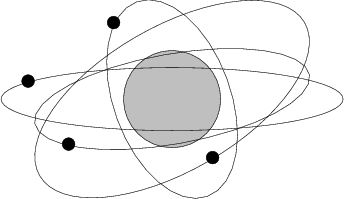
\epsfig{file={../fig/atome}}}   
 \caption{Planetary model of the atom: electrons revolve round the
   nucleus. This description is now replaced by the probabilistic description
   in the frame of quantum mechanics.}
 \label{figatome}
\end{figure}

\section{Molecules}
%%%%%%%%%%%%%%%%%%%%%%%%%
A molecule \cite{ph:mecaq:Cohen73,ph:mecaq:Pauling60} is an arrangement of some
atoms \index{molecule}(from two to some hundreds). Properties of molecules
can be described by quantum mechanics (see section \ref{secmolecmq}). The
knowledge of the geometry of a molecule is sometimes enough to understand its
properties. Figure \ref{figc60fig} represents fullerene molecule C60 at the
origin of chemistry Nobel price 1996 of Profs Curl, Kroto, et Smalley.
\begin{figure}[htb]
 \centerline{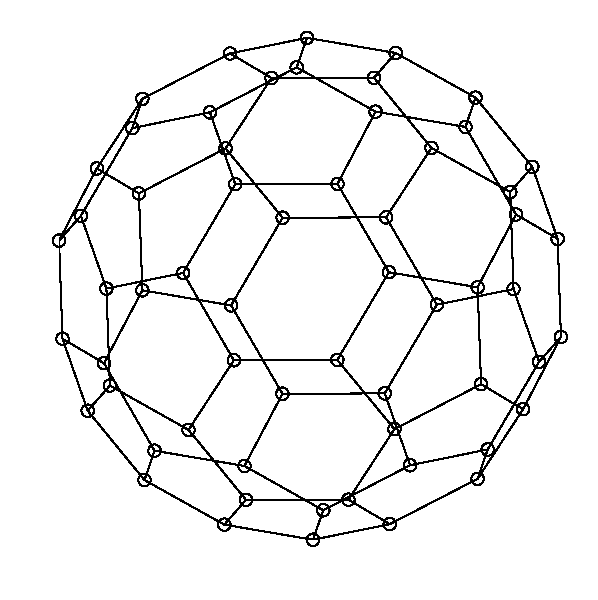
\epsfig{file={../fig/c60fig}}}   
 \caption{Fullerene C60 molecule (or footballene) is an example of a giant molecule.} 
 \label{figc60fig}
\end{figure}
Existence of such a molecule had been predicted by the study of the adsorption
spectrum of some distant stars.
Curl, Kroto, et Smalley succeeded in constructing it on the earth.  C60
molecule is compound by 12 pentagons and 20 hexagons.
It is the smallest spherical structure that can be construct using
polygons\index{fullerene}.  Polymers (see \cite{ph:ploym:Doi96}) are another
example of large molecules.
\section{Crystalline solids}
%%%%%%%%%%%%%%%%%%%%%%%%%%%%%%%%
Crystalline solids\cite{ph:solid:Kittel67,ph:solid:Ashcroft76} are  periodical
arrangement of atoms or molecules. \index{crystal}
Translation invariance symmetry allows to calculate approximations of quantum
states of such systems (see section \ref{secsolidmq}). 
Statistical physics allows to evaluate properties at equilibrium (see section
\ref{secgasparfq}). 
Continuous approximation allows to deal for instance with elasticity (see
sections \ref{sepripuiva} and \ref{secmaterelast}).  
Magnetic properties of solids are of great interest.
Solids can be classified according to the orientation of the magnetic
momentum carried by each elementary brick constituting  the solid (for
instance a small 
molecule) has a small magnetic moment \index{magnetic moment} or spin.
If orientation of those spins is random, crystal is said paramagnetic
\index{paramagnetic} (see figure~\ref{figparamag}). 
\begin{figure}[htb]
 \centerline{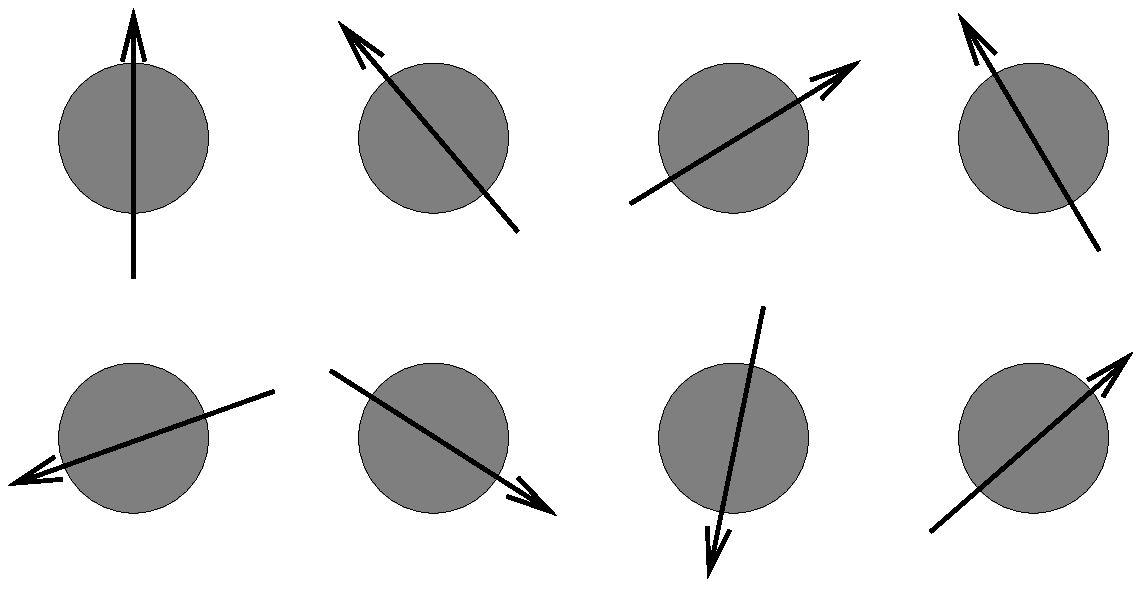
\epsfig{file={../fig/paramag}}}   
 \caption{In a paramagnetic solid, spins are random oriented, average
   magnetisation is thus zero.}
 \label{figparamag}
\end{figure}
Average magnetisation is then zero. If spins are oriented along a privileged
direction, crystal is called ferromagnetic \index{ferromagnetic}  (see
figure~\ref{figferromag}). There exists then a non zero magnetization.
\begin{figure}[htb]
 \centerline{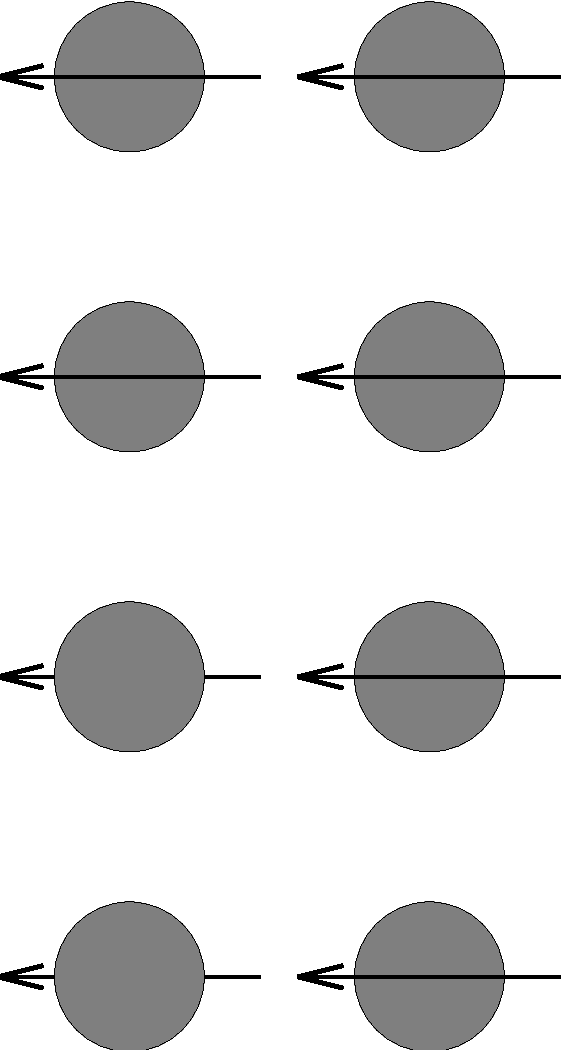
\epsfig{file={../fig/ferromag}}}   
 \caption{In a ferromagnetic crystal, spins are oriented along a
   privileged direction.}
 \label{figferromag}
\end{figure}
If spins have directions alternatively opposed (see
Figure~\ref{figantiferromag}), crystal is called anti ferromagnetic.
\begin{figure}[htb]
 \centerline{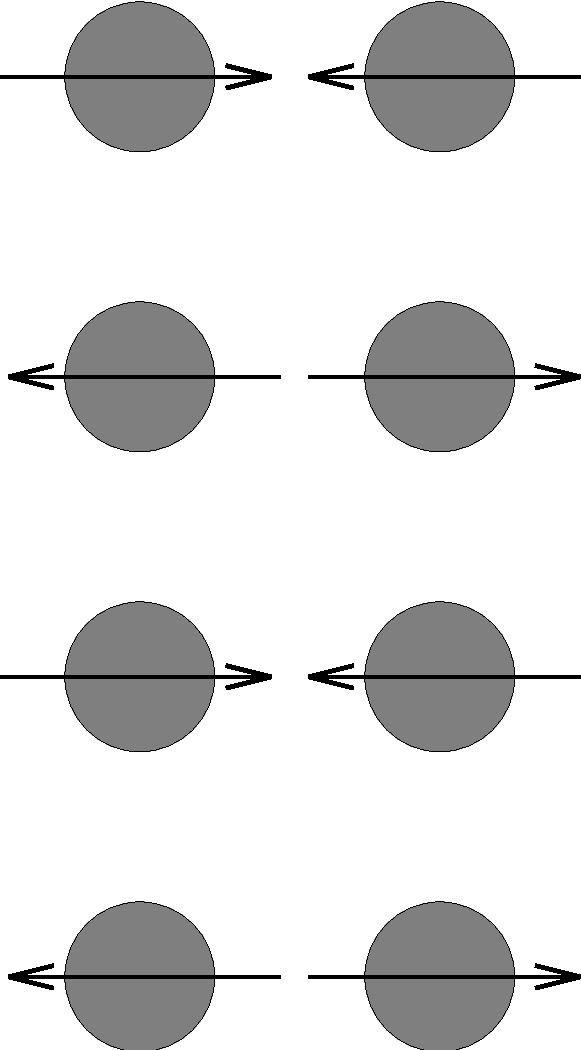
\epsfig{file={../fig/antiferromag}}}   
 \caption{In an anti ferromagnetic crystal, two neighbour spins are oriented in
   opposite directions.}
 \label{figantiferromag}
\end{figure}
Ising model, (see section \ref{secmodising}) is a simple model that allows to
describe 
{\bf paramagnetic -- ferromagnetic transition} that appears for certain
materials (for example iron) when temperature decreases.
\section{Gas and liquids}
%%%%%%%%%%%%%%%%%%%%%%%%%%%%%%
Gas\index{gas} and liquids \cite{ph:physt:Diu89} 
correspond to a random repartition of elementary bricks (atoms of
molecules). Gas particles are characterized by a large kinetic energy with
respect to the typical interaction energy between molecules.
When kinetic energy becomes of the same order than typical interaction energy
between molecules, gas transforms into liquid.
Van der Walls model allows to model the {\bf liquid
  vapor phase transition} (see section \ref{secvanderwaals}).
\section{Plasmas}
%%%%%%%%%%%%%%%%
A plasma\index{plasma} is a gas of ionized particle. Description of plasmas is
generally much more involved than description of classical gases (or
fluids). Indeed, the electromagnetic interaction plays here a
fundamental role, and in a fluid description of the system (see
chapter \ref{chapapproxconti}), fluid equations will be coupled to the
equations of the electromagnetic field (Maxwell equations). In
general, also, the nature of the particle can change after collisions.
Plasma state represents a large part of the ``visible'' matter (more than
99\%): indeed, all the stars are made of plasmas.

\section{Other matter arrangements}
%%%%%%%%%%%%%%%%%%%%%%%%%%%%%%%%%%%%%%%%%%
\subsection{Quasi crystals}
%%%%%%%%%%%%%%%%%%%%%%%%%%
Quasi crystals \cite{ph:quasi:Jaric88}
discovered by Israeli physicist  Shechtman in 1982 correspond to a non
periodical filling of a volume by atoms or molecules. Pentagon is a forbidden
form in crystallography: a volume can not be filled with elementary bricks of
fifth order symmetry repartited periodically. This problem has a two dimensional
twin problem: a surface can not be covered only by pentagons.
English mathematician Penrose \index{Penrose paving}discovered non
periodical paving 
of the  plane by lozenges of two types (see figure~\ref{figpenrose} and \ref{figpenrose2}). 
\begin{figure}[htb]
 \centerline{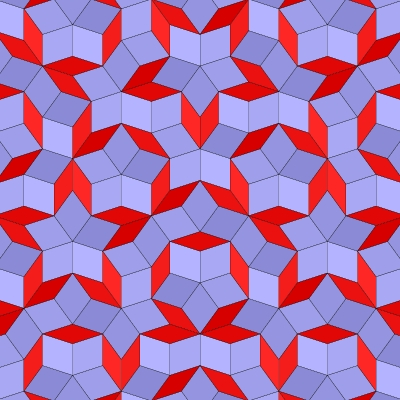
\epsfig{file={../fig/penrose}}}   
 \caption{Penrose paving: from two types of lozenges, non periodical paving of
   the plane can be constructed.}
 \label{figpenrose}
\end{figure}
\begin{figure}[htb]
 \centerline{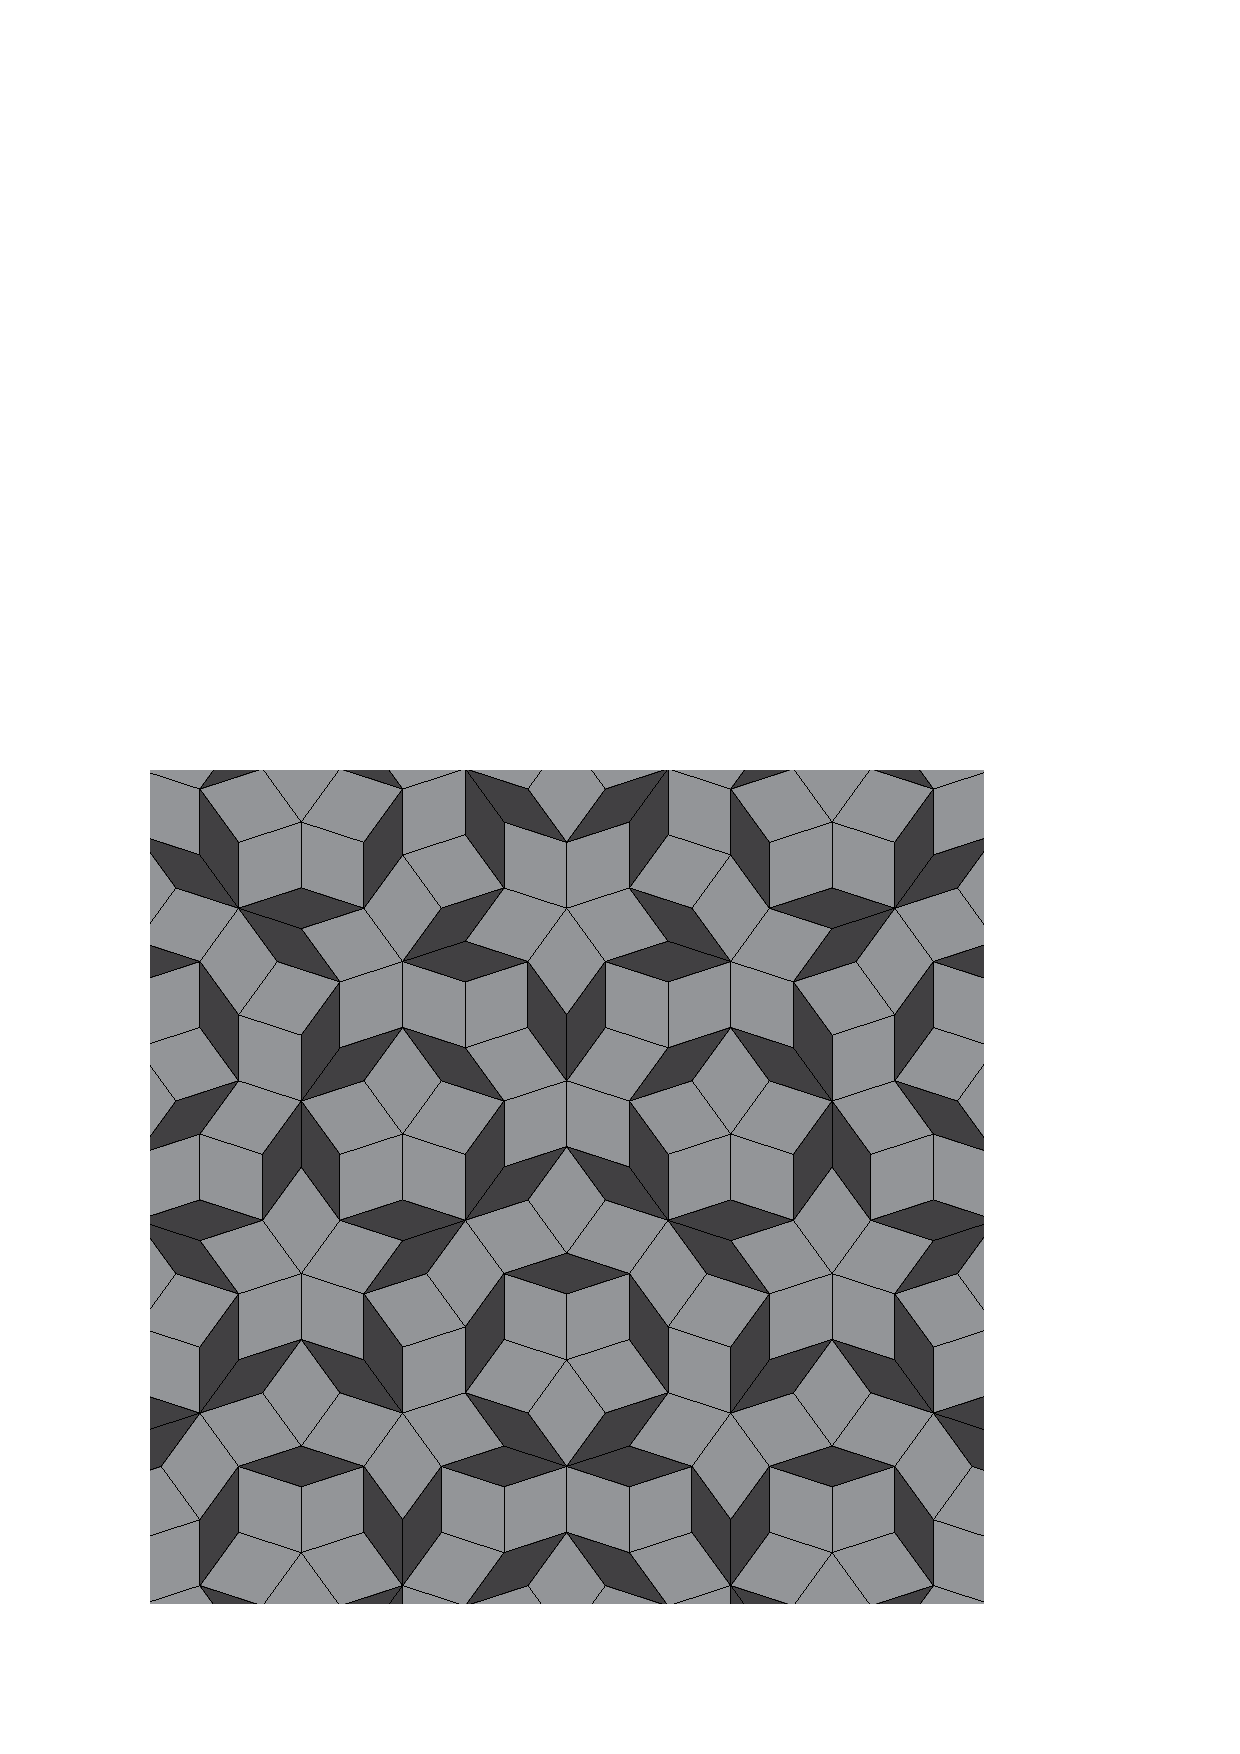
\epsfig{file={../fig/penrose2}}}   
 \caption{Penrose paving: same figure as previous one, but with only two gray
   levels to distinguish between the two types of lozenges.}
 \label{figpenrose2}
\end{figure}
Obtained structures are amazingly complex and it is impossible to
encounter some periodicity in the paving. 
\subsection{Liquid crystals}\label{secristliquides}
%%%%%%%%%%%%%%%%%%%%%%%%%%%%%%
Liquid crystals \cite{ph:liqcr:DeGennes74},
also called mesomorphic phases\index{mesomorphic phase}, are states
intermediary between the 
cristaline perfect order and the liquid disorder.
Molecules that compound liquid crystals\index{liquid crystal} have cigar--like
shape. They arrange themselves in space in order to form a ``fluid''
state more or less ordered.
Among the family of liquid crystals, several classes can be distinguished.
In the  {\bf nematic}\index{nematic} phase (see
figure~\ref{fignematique}), molecular axes stays parallel. There exists thus a
privileged direction. Each molecule can move with respect to its
neighbours, but in a fish ban way.
\begin{figure}[htb]
 \centerline{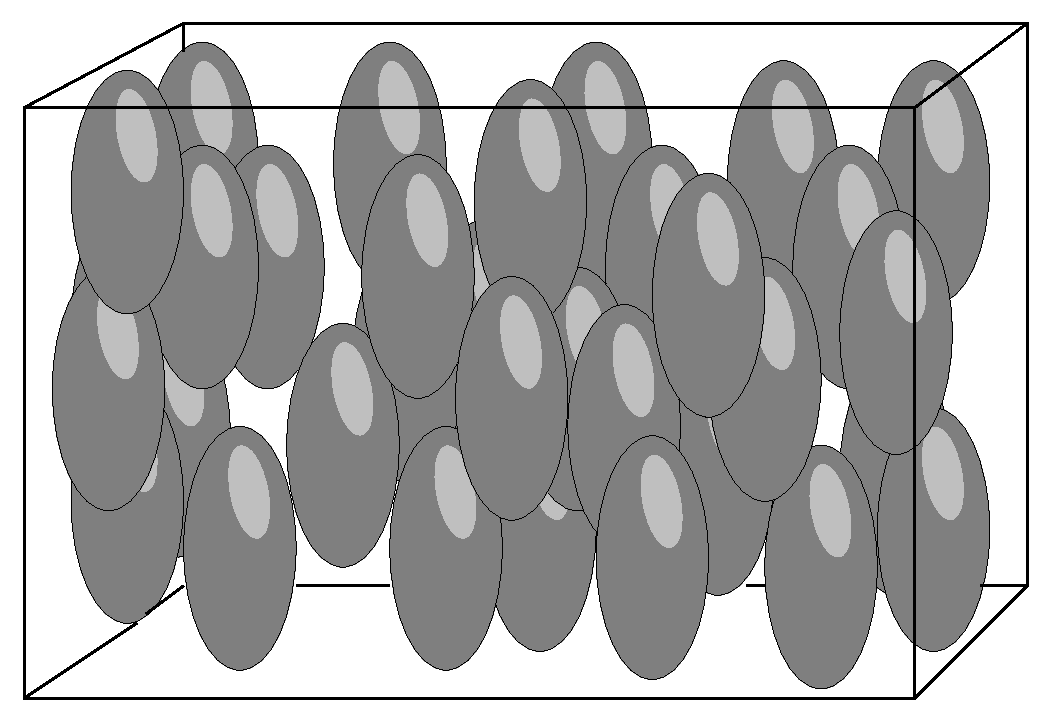
\epsfig{file={../fig/nematique}}}   
 \caption{Nematic material is similar to a fish ban: molecules have a
   privileged orientation and located at random points.}
 \label{fignematique}
\end{figure}
When molecules of a liquid crystal are not superposable to their image in a
mirror, a torsion of nematic structure appears: phase is then called 
{\bf cholesteric}\index{cholesteric}  (see
figure~\ref{figcholesteric}).
\begin{figure}[htb]
 \centerline{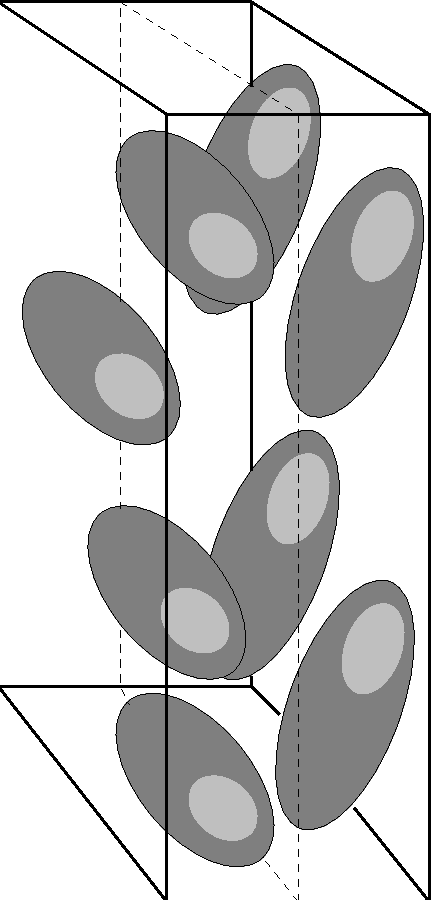
\epsfig{file={../fig/cholesteric}}}   
 \caption{In a cholesteric phase, molecules are arranged in layers. In each
   layer, molecule are oriented along a privileged direction. This direction
   varies from one layer to another, so that a helicoidal structure is
   formed.}
 \label{figcholesteric}
\end{figure}
{\bf Smectic}\index{smectic} phase is more ordered :
molecules are arranged in layers (see figure\ref{figsmectiqueA}). The fluid
character comes from the ability of layers to slide over their neighbours. 
\begin{figure}[htb]
 \centerline{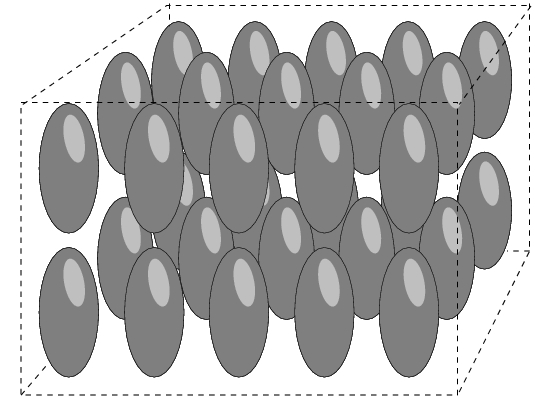
\epsfig{file={../fig/smectiqueA}}}   
 \caption{Smectic A}
 \label{figsmectiqueA}
\end{figure}
To describe deformations of nematics, a field of vector is used. To describe
deformations of smectics, each state is characterised by set of functions
$u_i(x,y)$ that describes the surface of the i$^{th}$ layer.
Energical properties of nematic materials are presented at section \ref{secenernema}.
\subsection{Colloids}
%%%%%%%%%%%%%%%%%%%%%
Colloids \index{colloid} are materials finely divided and
dispersed. Examples are emulsions \index{emulsion} and aerosols.
Consider a molecule that has two parts: a polar head which is soluble in
water and an hydrophobe tail. Such molecules are called
amphiphile\index{amphiphile molecule}. Once in
water, they gather into small structures called micelles\index{micelle}
(see figure 
\ref{fighuileeau}). Molecules turn their head to water and their tail to the
inside of the structure.
\begin{rem}
Cells of live world are very close to micelles, and it may be that
life\index{life (origin of)}\index{origin of life}
appeared by the mean of micelles.
\end{rem}

\begin{figure}[htb]
 \centerline{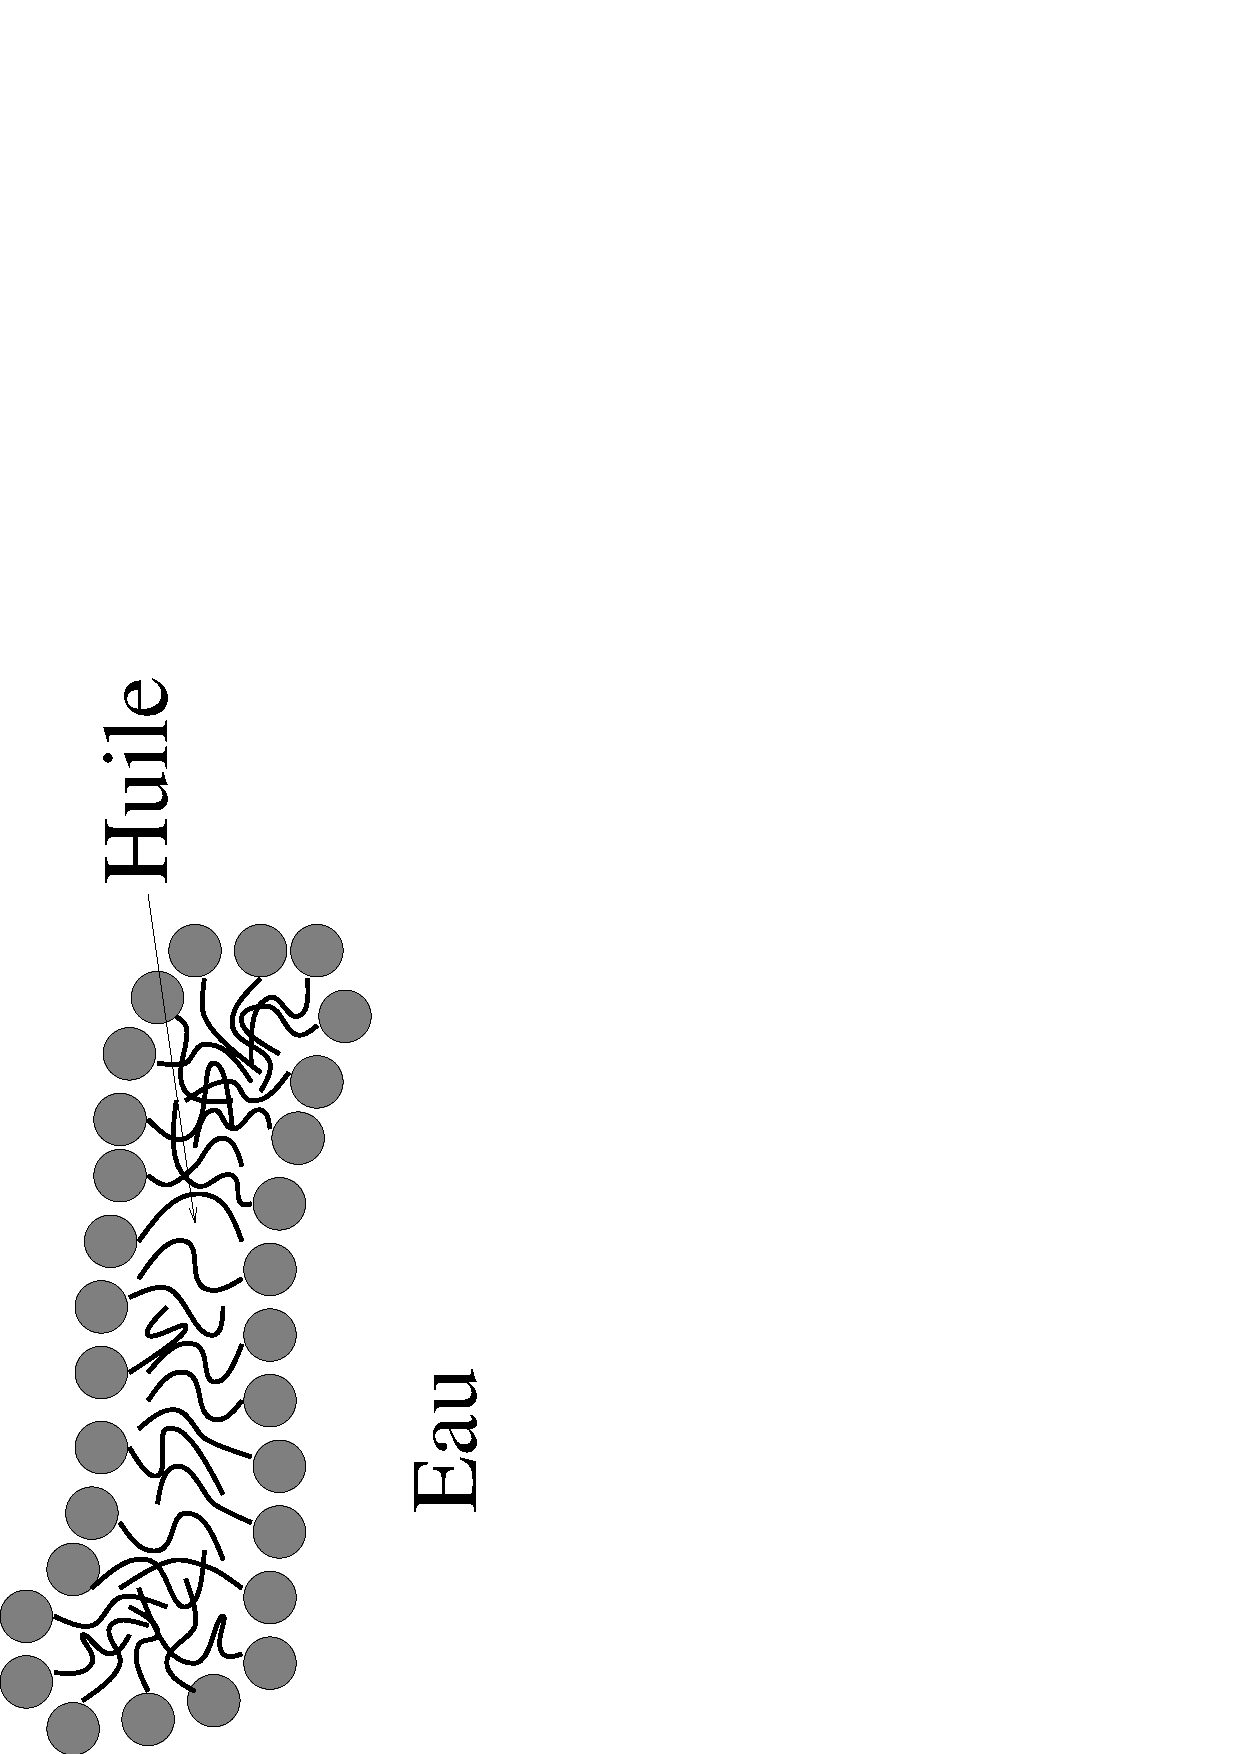
\epsfig{file={../fig/huileeau}}}   
 \caption{Amphiphile molecules (as oil molecules) that contains a hydrophile
   head and an hydrophobe tail organize themselves into small structures
   called micelles.}
\label{fighuileeau}
\end{figure}
Micelles can be encountered in mayonnaise
\cite{ph:cooki:Grosser81,ph:cooki:McGee84,ph:cooki:McGee90}.
Tensioactive substances allow to disolve micelles (application to soaps).
Foams are similar arrangements
\cite{ph:foams:Adamson76,ph:foams:Aubert86,ph:foams:Bikerman73}.
For a mathematical introduction to soap films and minimal surfaces,
check \cite{ma:equad:Morgan95}. 

\subsection{Glass}\label{secglassyspin}
%%%%%%%%%%%%%%%%%%
Glass state \cite{ph:mater:Zallen83} is characterized by a random distribution
of molecules (see figure
\ref{figglass}). Glass\index{glass} is solid, that implies that movements of
different constituents are small.
\begin{figure}[htb]
 \centerline{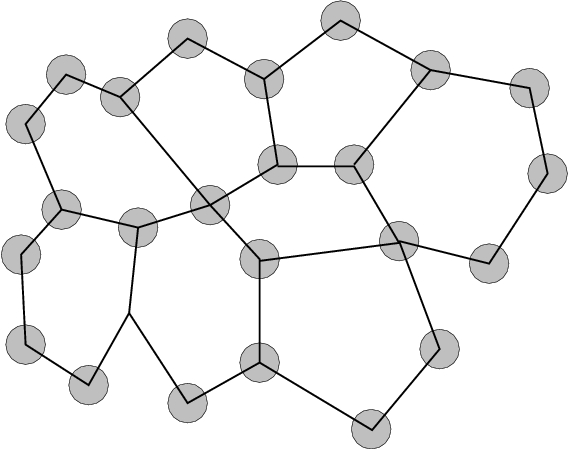
\epsfig{file={../fig/glass}}}   
 \caption{Glass is characterized by a great rigidity as crystals. However
   position of atoms are random.}
 \label{figglass}
\end{figure}
Phase transition between liquid state and glassy state is done progressively.
A material close to glass can be made by compressing small balls
together. Under pressure forces, those small balls are deformed and stick to
each other. Following question arises: are remaining interstices  
sufficiently numerous to allow a liquid to pour trough interstices ? This
pouring phenomena is a particular case of percolation
phenomenon\index{percolation} \cite{ph:mater:Zallen83}. Figure~\ref{figpercol}
illustrates this phenomenom in an experiment presented in \cite{ph:mater:Zallen83}.
\begin{figure}[htb]
 \centerline{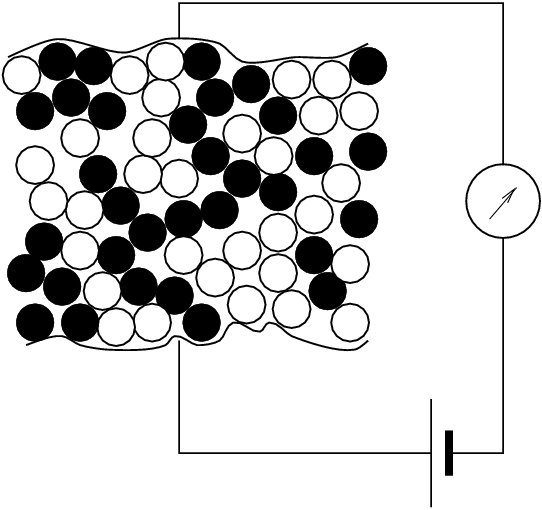
\epsfig{file={../fig/percol}}}   
 \caption{Example of percolation : black balls are conducting and white balls
   are insulating. Current running trough the circuit is measured as a
   function of proportion $p$ of white balls. There exists a critical
   proportion $p_c$ for which no more current can pass. Study of this critical
   point allows to exhibit some universal properties encountered in similar
   systems.}  
 \label{figpercol}
\end{figure}
Another example is given by the vandalized grid \cite{ph:mater:Zallen83} where
connections of a conducting wire is destroyed with probability $p$.

Spin glasses are disordered magnetic materials. A good example of spin glass
is given by the alloy coper manganese, noted CuMn where manganese atoms
carrying magnetic moments are dispersed at random in a coper matrix. two spins
tend to orient them selves in same or in opposite direction, depending on
distance between them (see figure~\ref{figspinglass}).
\begin{figure}[htb]
 \centerline{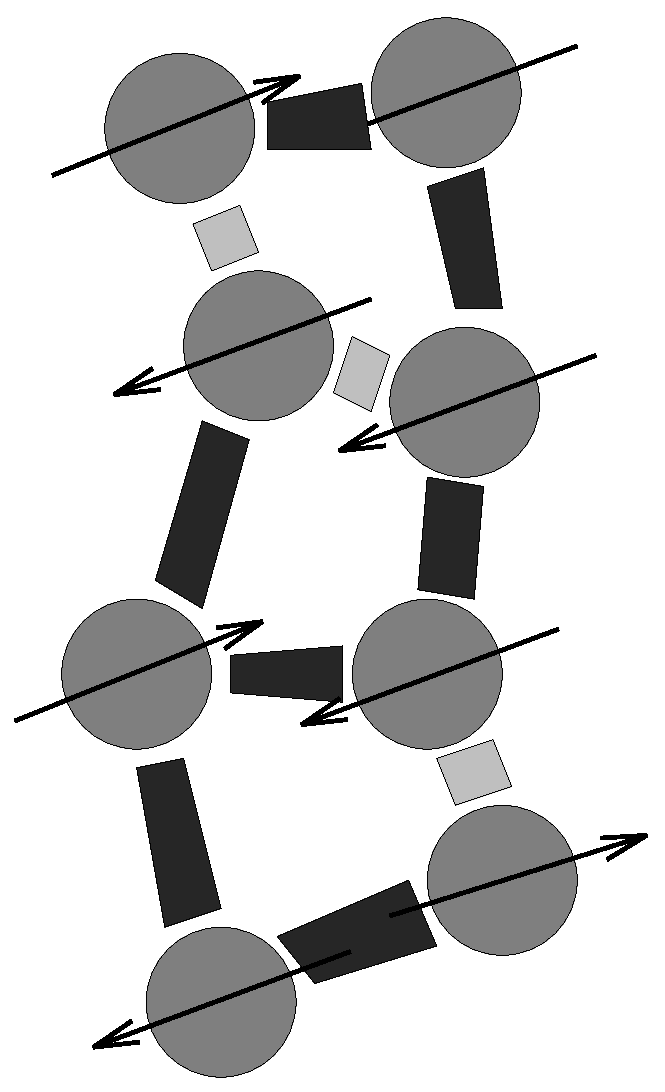
\epsfig{file={../fig/spinglass}}}   
 \caption{In a spin glass, interactions between neighbour spins are at random
   ferromagnetic type or anti ferromagnetic type, due to the random distance
   between spin sites.}
 \label{figspinglass}
\end{figure}
The resulting system is called ``frustrated'': there does not exist a
configuration for which all interaction energies are minimal. The simplest
example of frustrated system is given by a system constituted by three spins
labelled 1,2 and 3 where interactions obey the following rule:
energy decreases if 1 and 2 are pointing in the same direction, 2 and 3 are
pointing in the same direction and 1 and 3 are pointing in opposite direction.
Some properties of spin glasses are presented at section
\ref{secverredespi}.


\subsection{Sand piles, orange piles}
%%%%%%%%%%%%%%%%%%%%%%%%%%%%%%%%%%%%%%%
Physics of granular systems is of high interest and is now the subject of many
researches. Those systems, as a sand pile,  exhibit properties of both liquids
and solids. The sand in a hour-glass doesn't pour like liquids: the speed of
pouring doesn't depend on the high of sand above the hole. The formation of
the sand pile down of the hole is done by internal convection and avalanche
\index{avalanche} at the surface of the pile (see for instance
\cite{ph:granu:Guyon94}).

\section{Abstract}
%%%%%%%%%%%%%%%%
$N$ body problem is the fundamental problem of the modern description of
Nature. In this chapter we have shown through various examples the
variety of 
matter arrangement one can encounter in Nature.
We have noticed that, in general, among the four fundamental
interactions (strong 
interaction, weak interaction, electromagnetic interaction,
gravitation), gravitational and/or electromagnetic interactions are
relevant for the description of system of super nuclear scales that
are our interest in the rest of the book.
In the next two chapters, we will present the description of
gravitational and electromagnetic interactions.
\chapter{Relativity}\label{chaprelat}
%%%%%%%%%%%%%%%%
\section{Introduction}
%%%%%%%%%%%%%%%%%%%%%%
In this chapter we focus on the ideas of symmetry and
transformations. More precisely, we study the consequences on the
physical laws of transformation invariance. The reading of the
appendices \ref{chaptens} and \ref{chapgroupes} is thus recommended
for those who are not familiar with tensorial calculus and group theory.
In classical mechanics, a material point of mass $m$ is referenced by its
position $r$ and its momentum $p$ at each time $t$. Time does not depend on the
reference frame used to evaluate position and momentum. The
Newton's law of motion is invariant under Galileean
transformations. In special and general
relativity, time depends on the considered reference frame. This yields
to modify 
classical notions of position and momentum. Historicaly, special
relativity was proposed to describe the invariance of the light speed.
The group of transformations that leaves the new form of the dynamics
equations is the Lorentz group. Quantum, kinetic, and continuous
description of matter will be presented later in the
book.\footnote{%%%%%%%%%%%%%%%%%%%%%%%%%%%%%%%%
In quantum mechanics, physical space considered is a functional space, and the
state of a system is represented by a ``wave'' function $\phi(r,t)$ of space
and time. Quantity $|\phi(r,t)|^2dr$  can be interpreted as the probability to
have at time $t$ a particle in volume $dr$.
Wave function notion can be generalized to systems more complex than those
constituted by one particle.

A kinetic description of system constituted by an large number of particles
consists in representing the state of considered system by a function
$f(r,p,t)$ called ``repartition'' function, that represents the probability
density to encounter a particle at position  $r$ with momentum $p$.

Continuous description of matter refers to several functions of position and
time to describe the state of the physical system considered.}.%%%%%%%%%%%%

\section{Space geometrization}
%%%%%%%%%%%%%%%%%%%%%%%%%%%
\subsection{Classical mechanics}
%%%%%%%%%%%%%%%%%
Classical mechanics is based on two fundamental principles: the {\bf Galileo
  relativity} principle \index{Galileo relativity} and the
fundamental principle of dynamics.
Let us state Galileo relativity principle:
\begin{prin}
{\bf Galileo relativity principle.}
Classical mechanics laws (in particular Newton's law of motion) have
the same in every frame in uniform translation with respect to each
other. Such frames are called Galilean frames or inertial frames.
\end{prin}
In classical mechanics the time interval separing two events is
independant of the movement of the reference frame. Distance between two
points of a rigid body is independant of the movement of the
reference frame.

\begin{rem} Classical mechanics laws are invariant by transformations
  belonging to Galileo transformation group. A Galileo transformation
of coordinates can be written:
\begin{eqnarray}
x'_1&=&x_1-vt\\
x'_1&=&x_1\\
x'_1&=&x_1\\
t'&=&t
\end{eqnarray}
\end{rem}
Following Gallilean relativity, the light speed should depend on the
Galilean reference frame considered. In 1881, the experiment of Michelson
and Morley attempting to measure this dependance fails.


\subsection{Relativistic mechanics (Special relativity)}\label{secrelat} 
%%%%%%%%%%%%%%%%%%%%%%%%%%
Relativistic mechanics in the special case introduced by Einstein, as
he was 26 years old, is based on the following postulate: 
\begin{postulat}
All the laws of Universe ({\it i. e. }laws of mechanics and electromagnetism) are the same in all Galilean reference frames.
\end{postulat}
Because Einstein believes in the Maxwell equations (and because the
Michelson Morley experiment fails) $c$ has to be a constant. So
Einstein postulates:
\begin{postulat}
The light speed in vacuum $c$ is the same in every Galilean
reference frame. This speed is an upper bound.
\end{postulat}
We will see how the physical laws have to be modified to obey to
those postulates later on\footnote{The fundamental laws of dyanmics
is deeply modified (see section \ref{secdynasperel} (see section
\ref{secdynasperel})
, but as guessed by Einstein
Maxwell laws obey to the special relativity postulates (see section
\ref{seceqmaxcov}.
}.
The existence of a universal speed, the light speed, modifies deeply
space--time structure.
\index{space--time} It yields to precise the metrics\index{metrics}
 (see appendix \ref{chaptens} for an introduction to the notion of
metrics) adopted in special relativity. Let us consider two Galilean
reference frames characterized by coordinates:
$(x,t)$ and $(x^\prime,t^\prime)$. Assume that at $t=t^\prime=0$ both
coordinate system coincide. Then:
\begin{equation}
c=\frac{|x|}{|t|}=\frac{|x^\prime|}{|t^\prime|}
\end{equation}
that is to say:
\begin{equation}
c^2t^2-x^2=0
\end{equation}
and
\begin{equation}
c^2t^{\prime 2}-x^{\prime 2}=0
\end{equation}
Quantity $c^2t^2-x^2$ is thus an invariant.
The most natural metrics that should equip space--time is thus:
\begin{equation}
ds^2=dx^2+dy^2+dz^2-c^2dt^2
\end{equation}
It is postulated that this metrics should be invariant by Galilean change of
coordinates. 
\begin{postulat}
Metrics $ds^2=dx^2+dy^2+dz^2-c^2dt^2$ is invariant by change of Galilean
reference frame. 
\end{postulat}

Let us now look for the representation of a transformation of space--time that
keeps unchanged this metrics. We look for transformations such 
that:\index{Lorentz transformation}
\begin{equation}
ds^2=dx^2+dy^2+dz^2-c^2dt^2
\end{equation}
is invariant.
From, the metrics, a ``position vector'' have to be defined. It is called
four-vector position, and two formalisms are possible to define it:
\index{four--vector}.
\begin{itemize}
\item Either coordinates of four-vector position are taken equal to
$R=(x,y,z,ct)$ and space is equipped by pseudo scalar product defined by matrix:
\begin{equation}
D=
\left( \begin{array}{cccc}
1&0&0&0 \cr
0&1&0&0\cr
0&0&1&0\cr
0&0&0&-1\cr
\end{array} \right)
\end{equation}
Then:
\begin{equation}
(R|R)=R^tDR
\end{equation}
where $R^t$ represents the transposed of four-vector position $R$.
\item Or  coordinates of four-vector position are taken equal to
$R=(x,y,z,ict)$ and space is equipped by pseudo scalar product defined by
matrix: 
\begin{equation}
D=Id=
\left( \begin{array}{cccc}
1&0&0&0 \cr
0&1&0&0\cr
0&0&1&0\cr
0&0&0&1\cr
    \end{array} \right)      
\end{equation}
Then:
\begin{equation}
(R|R)=R^tR
\end{equation}
where $R^t$ represents the transposed four-vector position $R$.
\end{itemize}
Once the formalism is chosen, the representation of transformations ({\it
  i. e.,} the matrices), that leaves the pseudo-norm invariant can be
  investigated 
(see \cite{ph:relat:Misner73g}). Here we will just exhibit such matrices. In
first formalism, condition that pseudo-product scalar is invariant implies
that:
\begin{equation}
(MR|MR)=(R|R)
\end{equation}
thus
\begin{equation}
D=M^+DM
\label{cond}
\end{equation}
Following matrix suits:
\begin{equation}
M=
\left( \begin{array}{cccc}
\gamma&0&0&\gamma \beta \cr
0&1&0&0\cr
0&0&1&0\cr
\gamma \beta&0&0&\gamma\cr
         \end{array} \right)
\end{equation}
where $\beta=\frac{v}{c}$ ($v$ is the speed of the reference frame) and
$\gamma=\frac{1}{\sqrt{1-\beta^2}}$. 
The inverse of $M$:
\begin{equation}
M^{-1}=
\left( \begin{array}{cccc}
\gamma&0&0&-\gamma \beta \cr
0&1&0&0\cr
0&0&1&0\cr
-\gamma \beta&0&0&\gamma\cr
          \end{array} \right)
\end{equation}
\begin{rem}
Equation \ref{cond} implies a condition for the determinant:
\begin{equation}
1=det(M^+DM)=(det(M))^2
\end{equation}
Matrices $M$ of determinant 1 form a group called Lorentz group.
\index{Lorentz group}
 \end{rem}
In the second formalism, this same condition implies:
\begin{equation}
Id=M^+M
\end{equation}
Following matrix suits:
\begin{equation}
M=
\left( \begin{array}{cccc}
\gamma&0&0&-i\gamma \beta \cr
0&1&0&0\cr
0&0&1&0\cr
+i\gamma \beta&0&0&\gamma\cr
          \end{array} \right)
\end{equation}
and its inverse is:
\begin{equation}
M^{-1}=
\left( \begin{array}{cccc}
\gamma&0&0&+i\gamma \beta \cr
0&1&0&0\cr
0&0&1&0\cr
-i\gamma \beta&0&0&\gamma\cr
\end{array} \right)          
\end{equation}
\begin{rem}
A unitary matrix (see section \ref{secautresrep}) is a matrix such that:
\begin{equation}
M^+M=1=MM^+
\end{equation}
where $M^+$ is the adjoint matrix of $M$, that is the conjugated transposed
matrix of $M$. Then, scalar product defined by:
\begin{equation}
 \mathrel{<} R|Q\mathrel{>} =R^+Q
\end{equation}
is preserved by the action of $M$.
\end{rem}

\subsubsection{Eigen time}
Four-scalar (or Lorentz invariant) $d\tau$ allows to define other
four-vectors (as four-vector velocity):
\begin{defn}
Eigen time of a mobile is time marked by a clock travelling with this mobile.
\end{defn}
If mobile travels at velocity $v$ in reference frame $R_2$, then events A and B
that are referenced in $R_1$ travelling the mobile by:
\begin{eqnarray}
x_A=0& &x_B=0\\
ct_A=0& &ct_B=c\tau
\end{eqnarray}
and are referenced in $R_2$ by:
\begin{eqnarray}
x_A=0& &x_B=vt\\
ct_A=0& &ct_B=ct.
\end{eqnarray}
So, one gets the relation verified by $\tau$::
\begin{equation}
\tau^2=t^2(1-\frac{v^2}{c^2})
\end{equation}
so
\begin{equation}
d\tau=\frac{dt}{\gamma}
\end{equation}

\subsubsection{Velocity four-vector}
%%%%%%%%%%%%%%%%%%%%%%%%
Velocity four-vector is defined by:
\begin{equation}
U=\frac{dX}{d\tau}=(\gamma u,\gamma c)
\end{equation}
where $u=\frac{dx}{dt}$ is the classical speed.
\subsubsection{Other four-vectors}
%%%%%%%%%%%%%%%%%%%%%%%%
Here are some other four-vectors (expressed using first formalism):
\begin{itemize}
\item four-vector position :
\begin{equation}
X=(x_1,x_2,x_3,ct)
\end{equation}
\item four-vector wave:
\begin{equation}
K=(k_1,k_2,k_3,\frac{\omega}{c})
\end{equation}
\item four-vector nabla:
\begin{equation}
K=(\frac{\partial}{\partial x_1},\frac{\partial}{\partial x_2},\frac{\partial}{\partial x_3},\frac{\partial}{\partial x_4})
\end{equation}
\end{itemize}


\subsection{General relativity}
%%%%%%%%%%%%%%%%%%%%%%%%%%%%
There exists two ways to tackle laws of Nature discovery problem: 
\begin{enumerate}
\item First method can be called {
``phenomenological''}. A good example of phenomenological theory is quantum
mechanics theory. This method consists in starting from known facts (from
experiments) to infer laws. Observable notion is then a fundamental notion.
\item There exist another method less ``anthropocentric'' whose advantages had
  been underlined at century 17 by philosophers like Descartes. 
It is the method called {\it a priori}. It has been used by Einstein to propose
his relativity theory. It consists in starting from principles that are
believed to be true and to look for laws that obey to those principles.
\end{enumerate}
Here are the fundamental postulates of general relativity:
\begin{postulat}
{\bf Generalized relativity principle}:
All the laws of Nature are covariant\index{covariance} relatively to any
continuous transformation of coordinates system.
\footnote{Special relativity states only covariance with respect to Lorentz
  transformations (see \cite{ph:relat:Misner73g}) and classical
  mechanics states covariance only under Galilean transformations.}
\end{postulat}
\begin{postulat}
{\bf Maximum logical simplicity principle for laws formulation:}
All {\bf geometrical} properties of space--time can be described by the means
of a differential tensor $S$. This tensor 
\begin{enumerate}
\item is expressed in a four dimension Riemannian space whose metrics is
  defined by a tensor $g_{ij}$
\item is a second order tensor and is noted $S_{ij}$
\item is a function of the $g_{ij}$'s that doesn't contain any partial
  derivatives of order greater than two and that is linear with respect to
  second order partial derivatives.
\end{enumerate}
\end{postulat}
\begin{postulat}
Divergence of tensor $S_{ij}$ is zero.
\end{postulat}
\begin{postulat}
Space curvature is due to matter:
\begin{equation}
\mbox{ Curvature }=\mbox{ Matter }
\end{equation}
or, using tensors:
\begin{equation}
S_{ij}=T_{ij}
\end{equation}
\end{postulat}
Einstein believes strongly in those postulates. On another hand, he believes
that modelization of gravitational field have to be improved.
From this postulates, Einstein equation can be obtained: One can show that any
tensor $S_{ij}$ that verifies those postulates:
\begin{equation}
S_{ij}=a(R_{ij}-\frac{1}{2}g_{ij}R-\lambda g_{ij})
\end{equation}
where $a$ and $\lambda$ are two constants and  $R_{ij}$, the Ricci
curvature tensor, and $R$, the scalar curvature are defined from $g_{ij}$
tensor\footnote{%%%%%%%%%%%
Reader is invited to refer to specialized books for the expression of
$R_{ij}$ and $R$.}%%%%%%%%%%%%
Einstein equation corresponds to $a=1$. Constant $\lambda$ is called
cosmological constant. Matter tensor is not deduced from symmetries implied by
postulates as tensor $S_{ij}$ is. Please refer to
\cite{ph:relat:Misner73g} for indications about how to model
matter tensor. Anyway, there is great difference between $S_{ij}$ curvature
tensor and matter tensor. Einstein opposes those two terms saying that
curvature term is smooth as gold and matter term is rough as wood.
\section{Dynamics}
%%%%%%%%%%%%%%
\subsection{Fundamental principle of classical mechanics}
%%%%%%%%%%%%%%%%%%%%%%%%%%%%%%%
Let us state fundamental principle of classical dynamics for material
point\footnote{%%%%%%%
Formulation adapted to continuous matter will be presented later in the book.
}.%%%%%
A material point is classically described by its mass $m$, its position $r$,
and its velocity $v$. 
It undergoes external actions modelized by forces $F_{ext}$. Momentum $mv$ of
the particle  is noted $p$.\index{momentum}
\begin{prin}
Dynamics fundamental principle or (Newton's equation of motion)
\index{Newton's equation of motion}
 states that the time derivative of momentum is equal to the sum
of all external forces\index{force}:
\begin{equation}
\frac{dp}{dt}=\sum F_{ext}
\end{equation}
\end{prin}
\subsection{Least action principle}\label{secprinmoindreact}
%%%%%%%%
\begin{prin}{\bf Least action principle:}
\index{least action principle} 
Function $x(t)$ describing the trajectory of a particle in a potential
$U(x)$ in a potential $U(x)$ yields the action stationary, where the action $S$ is defined
by $S=\int L dt$ where $L$ is the Lagrangian of the particle: 
$L(x,\dot x,t)=-\frac{1}{2}m\dot x ^2+U(x)$. 
\end{prin}
This principle can be taken as the basis of material point classical
mechanics. But it can also be seen as a consequence of fundamental dynamics
principle presented previously\cite{ma:equad:Arnold83}.
\begin{equation}
m \ddot{x}+\frac{\partial U}{\partial x}=0
\end{equation}
Let us multiply by $y(t)$ and integrate over time:
\begin{equation}
\int (m \ddot{x}y +\frac{\partial U}{\partial x}y)\,dt=0
\end{equation}
Using Green theorem (integration by parts):
\begin{equation}
\int (-m \dot{x}\dot{y} +\frac{\partial U}{\partial x}y)\,dt=0
\end{equation}
$\dot{x}\dot{y}$ is a bilinear form.
\begin{equation}
-\dot{x}\dot{y}=-\frac{\partial }{\partial x}\frac{1}{2}\dot{x}^2
\end{equation}
\begin{equation}
0= \int m
[-\frac{1}{2}(\dot{x}+\dot{y})^{2}+U(x+y)]
-[-\frac{1}{2}\dot{x}^{2}+U(x)]dt+O(y^{2}) 
\end{equation}
Defining Lagrangian $L$ by:
\begin{equation}
L(\dot{x},x,t)=-\frac{1}{2}m\dot x ^2+U(x),
\end{equation}
previous equation can be written
\begin{equation}
0=-\delta \int L(\dot{x},x,t)dt
\end{equation}
meaning that action $S$ is stationary.
\subsection{Description by energies}
%%%%%%%%%%%%%%%%%%%%%%%%%%%%%%%%%%%%%%%%%%%
Laws of motion does not tell anything about how to model
forces. The force modelization is often physicist's job. Here are two
examples of 
forces expressions:  
\begin{enumerate}
\item weight $P=mg$. $g$ is a vector describing gravitational field around the
  material point of mass $m$ considered.
\item electromagnetic force $f=qv\wedge B+qE$, where $q$ is particle's
  charge, $E$ is the electric field, $B$ the magnetic field and $v$ the
  particle's velocity.
\end{enumerate} 
This two last forces expressions directly come from physical
postulates. However, for other interactions like elastic forces, friction,
freedom given to physicist is much greater.

An efficient method to modelize such complex interactions is to use the energy
(or power) concept. At chapter \ref{chapelectromag}, the duality between
forces and energy is presented in the case of electromagnetic interaction.
At chapters \ref{chapapproxconti} and \ref{chapenermilcon}, the concept of
energy is developed for the description of continuous media.

Let us recall here some definitions associated to the description of
interactions by forces. Elementary work of a force $f$ for an elementary
displacement is:
\begin{equation}
\delta W=f.dr
\end{equation}
Instantaneous power emitted by a force $f$ to a material point of velocity $v$
is: 
\begin{equation}
P=f.v
\end{equation}
Potential energy gained by the particle during time $dt$ that it needs to move
of $dr$ is:
\begin{equation}
dE=-f.dr=-P.dt
\end{equation}
Note that potential energy can be defined only if force field $f$ have
conservative circulation\footnote{%%%%%%%%%%%
That means:
\begin{equation}
\int_C f.dr=0
\end{equation}
for every loop $C$, or equivalently that
\begin{equation}
\mbox{ rot } f=0.
\end{equation}
}%%%%%%%%%%%%%
. This is the case for weight, for electric force but not for friction. A
system that undergoes only conservative forces is hamiltonian. The equations
that govern its dynamics are the Hamilton equations:
\begin{equation}\label{eqhampa1}
\frac{dp}{dt}=-\frac{\partial H}{\partial q}
\end{equation}
\begin{equation}\label{eqhampa2}
\frac{dq}{dt}=\frac{\partial H}{\partial p}
\end{equation}
where function $H(q,p,t)$ is called hamiltonian of the system. For a particle
with a potential energy $E_p$, the hamiltonian is:
\begin{equation}\label{eqformhami}
H(q,p,t)=\frac{p^2}{2m}+E_p(q)
\end{equation}
where $p$ is particle's momentum and $q$ its position.
By extension, every system whose dynamics can be described by equations
\ref{eqhampa1} and \ref{eqhampa2} is called hamiltonian
\index{hamiltonian system}
even if $H$ is not of the form given by equation
\ref{eqformhami}. 

\subsection{Dynamics in special relativity}\label{secdynasperel}
%%%%%%%%%%%%%%%%%%
It has been seen that Lorentz transformations acts on time. Classical dynamics
laws have to be modified to take into into account this fact and maintain
their invariance under Lorentz transformations as required by relativity
postulates. Price to pay is a modification of momentum and energy notions.
Let us impose a linear dependence between the impulsion four-vector and
velocity four-vector;
\begin{equation}
P=mU=(m\gamma u,icm\gamma)
\end{equation}
where $m$ is the rest mass of the particle, $u$ is the classical speed
of the particle $u=\frac{dx}{dt}$,
$\gamma=\frac{1}{\sqrt{1-\beta^2}}$, with $\beta=\frac{u}{c}$. Let us
call ``relativistic 
momentum'' quantity:
\begin{equation}
p=m \gamma u
\end{equation}
and ``relativistic energy'' quantity:
\begin{equation}
E=m\gamma c^2
\end{equation}
Four-vector $P$ can thus be written:
\begin{equation}
P=(p,i\frac{E}{c})
\end{equation}
Thus, Einstein associates an energy to a mass since at rest: 
\begin{equation}
E=mc^2
\end{equation}
This is the {\bf matter--energy equivalence}.
\index{matter--energy equivalence}
Fundamental dynamics principle is thus written in the special relativity
formalism:
\begin{equation}
\frac{dP}{dt}=f_\mu
\end{equation}
where $f_\mu$ is force four-vector.
\begin{exmp}
Let us give an example of force four-vector. Lorentz force four-vector is
defined by:
\begin{equation}
f^\mu=F^\mu_\nu P^\mu
\end{equation}
where $F^\mu_\nu$ is the electromagnetic tensor field  (see section
\ref{seceqmaxcov}) 
\end{exmp}
\subsection{Least action principle in special relativity}
%%%%%%%%%%%%%%%%%%%%%%%%%%%%%%%%%%%%%%%%%
Let us present how the fundamental dynamics can be retrieved from a
least action principle. Only the case of a free particle is
considered.
Action should be written:
\begin{equation}
S=\int L(u,x,t) dt
\end{equation}
where $L$ is invariant by Lorentz transformations, $u$ and $x$ are the
classical speed and position of the particle. The simplest
solution consists in stating:
\begin{equation}
L=\gamma k
\end{equation}
where $k$ is a constant. Indeed $Ldt$ becomes here:
\begin{equation}
Ldt=k d\tau
\end{equation}
where $d\tau=\frac{dt}{\gamma}$, 
(with $\gamma=\frac{1}{\sqrt{1-\beta^2}}$, and 
$\beta=\frac{u}{c}$) is the differential of the
eigen time and is thus 
invariant under any Lorentz transformation. Let us postulate that $k=-mc^2$.
Momentum is then:
\begin{equation}
p=\frac{\partial L}{\partial u}=\gamma m u
\end{equation}
Energy is obtained by a Legendre transformation, $E=p.u-L$ so:
\begin{equation}
E=\gamma m c^2
\end{equation}


\subsection{Dynamics in general relativity}
%%%%%%%%%
The most natural way to introduce the dynamics of a free particle in
general relativity is to use the least action principle.
Let us define the action $S$ by:
\begin{equation}
S=\int ds
\end{equation}
where $ds$ is the elementary distance in the Rieman space--time
space. $S$ is obviously covariant under any frame transformation
(because $ds$ does). 
Consider the fundamental relation \ref{eqcovdiff} that defines
(covariant) differentials. It yields to:
\begin{equation}
Da^i=da^i+a^k\Gamma^i_{kj}dx^j
\end{equation}
where $da^i=\frac{\partial a^i}{\partial x^j}dx^j$.
A deplacement can be represented by $dx^i=u^id\lambda$ where $u^i$
represents the tangent to the trajectory (the velocity). 
The shortest path corresponds to a movement of the particle such the
the tangent is transported parallel to itself, that is\footnote{The
actual proof that action $S$ is minimal implies that $DU^i=0$ is given
in \cite{ph:relat:Misner73g,ma:tense:Brillouin64}}%%%%%%%
:
\begin{equation}
Du^i=0.
\end{equation}
or 
\begin{equation}
\frac{Du^i}{d\lambda}=0
\end{equation}
This yields to
\begin{equation}\label{eqdynarelatge} 
\frac{D u^i}{D\lambda}=\frac{d^2x^i}{d\lambda^2}+\Gamma^{i}_{hk}
\frac{dx^h}{d\lambda} \frac{dx^k}{d\lambda} 
\end{equation}
where $\Gamma^{i}_{hk}$ is tensor depending on system's metrics (see
\cite{ph:relat:Misner73g} for more details).
Equation \ref{eqdynarelatge} is an evolution equation for a free
particle. It is the equation of a geodesic. Figure \ref{figgeo}
represents the geodesic between two point A and B on a curved space
constituted by a sphere. In this case the geodesic is the arc binding
A and B. 

\begin{figure}[htb]
 \centerline{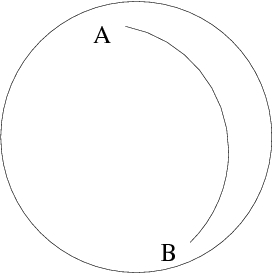
\epsfig{file={../fig/geodesic}}}   
 \caption{Geodesic on a sphere.} 
 \label{figgeo}
\end{figure}
Note that here, gravitational interaction is contained in the
metrics. So the equation for the ``free'' particle above describes the
evolution of a particle undergoing the gravitational interaction.
General relativity explain have larges masses can deviate light rays
(see figure \ref{figlightrayd})
\begin{figure}[htb]
 \centerline{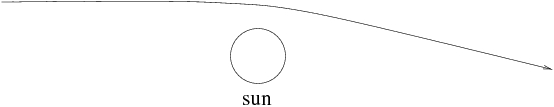
\epsfig{file={../fig/lightdev}}}  
 \caption{Curvature of a light .} 
 \label{figlightrayd}
\end{figure}

\section{Exercises}
%%%%%%%%%%%%%%%%%%%%
\begin{exo}
Show that a rocket of mass $m$ that ejects at speed $u$ (with respect to
itself) a part of its mass $dm$ by time unit $dt$ moves in the sense opposed
to $u$. Give the movement law for a rocket with speed zero at time $t=0$,
located in a earth gravitational field considered as constant. 
\end{exo}

\begin{exo}
{\bf Doppler effect.} Consider a light source $S$ moving at constant speed
with respect to reference frame $R$. Using wave four-vector $(k,\omega/c)$ give
the relation between frequencies measured by an experimentator moving with $S$
and another experimentater attached to $R$. What about sound waves?
\end{exo}

\begin{exo}
For a cylindrical coordinates system, metrics $g_{ij}$ of the space is:
\begin{equation}
ds^2=dr^2+r^2d\theta^2+dz^2
\end{equation}
Calculate the Christoffel symbols $\Gamma^{i}_{hk}$ defined by:
\begin{equation}
\Gamma^{i}_{hk}=\frac{1}{2}g^{ij} (\partial_hg_{kj}+ \partial_kg_{hj}-
\partial_jg_{hk})
\end{equation}
\end{exo}
\begin{exo}
Consider a unit mass in a three dimensional reference frame whose metrics is:
\begin{equation}
ds^2=g_{ij}dq_idq_j
\end{equation}
Show that the kinetic energy of the system is:
\begin{equation}
E_c=\frac{1}{2}g_{ij}\dot q_i\dot q_j
\end{equation}
Show that the fundamental equation of dynamics is written here (forces are
assumed to derive from a potential $V$) :
\begin{equation}
\frac{D\dot q_i}{Dt}=-\frac{\partial V}{\partial q_i}
\end{equation}
\end{exo}

\chapter{Electromagnetism}\label{chapelectromag}
%%%%%%%%%%%%%%%%%%%%%%%%%%%%%%%
\section{Introduction}
%%%%%%%%%%%%%%%%%%%%%
At previous chapter, equations that govern dynamics of a particle in a
filed of forces where presented. In this chapter we introduce
electromagnetic forces.  
Electromagnetic interaction is described by the mean of electromagnetic
field, which is solution of so-called Maxwell equations. But as Maxwell
equations take into account positions of sources (charges and currents), we
have typically coupled dynamics--field equations problem: fields act on
charged particles and charge particles act on fields.

A first way to solve this problem is to study the static case. A second way is
to assume that particles able to move have a negligible effect on the
electromagnetic field distribution (assumed to be created by some ``big''
static sources). The last way is to tackle directly the coupled equations
system (this is the usual way to treat plasma problems, see exercise
\ref{exoplasmapert} and reference \cite{ph:plasm:Chen84}).

This chapter presents Maxwell equations as well as their applications to
optics. Duality between representation by forces and by powers of
electromagnetic interaction is also shown.
 
\section{Electromagnetic field}
%%%%%%%%%%%%%%%%%%%%%%%%%%%
\subsection {Equations for the fields: Maxwell equations}
%%%%%%%%%%%%%%%%%%%%%%%%%%%%
Electromagnetic interaction is described by the means of Electromagnetic
fields: $E$ field called electric field, $B$ field called magnetic field, $D$
field and $H$ field.
Those fields are solution of Maxwell equations,
\index{Maxwell equations}
\begin{equation}
\mbox{ div } D=\rho
\end{equation}
\begin{equation}
\mbox{ rot } H=j+\frac{\partial{D}}{\partial t}
\end{equation}
\begin{equation}
\mbox{ div } B=0
\end{equation}
\begin{equation}
\mbox{ rot } E=-\frac{\partial B}{\partial t}
\end{equation}
where  $\rho$ is the charge density and $j$ is the current density. This
system of equations has to be completed by additional relations called
constitutive relations that bind $D$ to $E$ and $H$ to $B$. 
In vacuum, those relations are:
\begin{equation}
D=\epsilon_0E
\end{equation}
\begin{equation}
H=\frac{B}{\mu_0}
\end{equation}
In continuous material media, energetic hypotheses should be done (see
chapter \ref{parenergint}) .
\begin{rem}
In harmonical regime\footnote{%%%%%
That means that fields satisfy following relations:
\begin{equation}
E={\cal E}e^{j\omega t}
\end{equation}
\begin{equation}
B={\cal B}e^{j\omega t}
\end{equation}
}%%%%%%
and when there are no sources and when constitutive relations are:
\begin{itemize}
\item for $D$ field
\begin{equation}
D(r,t)=\epsilon(r,t) * E(r,t)
\end{equation}
where $*$ represents temporal convolution\index{convolution} (value of
$D(r,t)$ field at time $t$ 
depends on values of $E$ at preceding times) and:
\item for $B$ field:
\begin{equation}
H=\frac{B}{\mu_0},
\end{equation}
\end{itemize}
Maxwell equations imply Helmholtz equation:
\begin{equation}
\Delta {\cal E}+k^2 {\cal E}=0.
\end{equation}
Proof of this is the subject of exercise
\ref{exoeqhelmoltz}.
\end{rem}
\begin{rem}
Equations of optics are a limit case of Maxwell equations. Ikonal equation:
\begin{equation}
\mbox{ grad }^2 L=n^2
\end{equation}    
where $L$ is the optical path and $n$ the optical index is obtained from the
Helmholtz equation using WKB method (see section \ref{secWKB}). Fermat
principle can be deduced from ikonal equation {\it via} equation of light ray
(see section \ref{secFermat}). Diffraction's Huyghens principle can be deduced
from Helmholtz equation by using integral methods (see section
\ref{secHuyghens}). 
\end{rem} 




\subsection{Conservation of charge}
%%%%%%%%%%%%%%%%%%%%%%%%%%%%%%%%%%
Local equation traducing conservation of electrical charge is:
\begin{equation}\label{eqconsdelacharge}
\frac{\partial \rho}{\partial t}+\mbox{ div }{j}=0
\end{equation}
\subsection{Modelization of charge}\label{secmodelcha}
%%%%%%%%%%
Charge density in Maxwell-Gauss equation in vacuum 
\begin{equation}
\mbox{ div } E=\frac{\rho}{\epsilon_0}
\end{equation}
has to be taken in the sense of distributions, that is to say that $E$ and
$\rho$ are distributions. In particular $\rho$ can be Dirac distribution, and
$E$ can be discontinuous (see the appendix \ref{chapdistr} about
distributions). 
By definition:
\begin{itemize}
\item a point charge  $q$ located at  $r=0$ is modelized by the distribution
  $q\delta(r)$ where $\delta(r)$ is the Dirac distribution.
\item a dipole\index{dipole} of dipolar momentum $P_i$ is modelized by
  distribution $\mbox{ div }(P_i\delta(r))$. 
\item a quadripole of quadripolar tensor\index{tensor}
$Q_{i,j}$ is modelized by distribution
$\partial_{x_i}\partial_{x_j}(Q_{i,j}\delta(r))$. 
\item in the same way, momenta of higher order can be defined.
\end{itemize}
Current density $j$ is also modelized by distributions:
\begin{itemize}
\item the monopole doesn't exist! There is no equivalent of the point charge.
\item the magnetic dipole is $\mbox{ rot } A_i\delta(r)$
\end{itemize}
\subsection{Electrostatic potential}\label{secpotelec}
%%%%%%%%%%%%%%%%%%%%%%
Electrostatic potential is solution of Maxwell-Gauss equation:
\begin{equation}
\Delta V=\frac{\rho}{\epsilon_0}
\end{equation}
This equations can be solved by integral methods exposed at section
\ref{chapmethint}: once the Green solution of the problem is found (or the
elementary solution for a translation invariant problem), solution for any
other source can be written as a simple integral (or as a simple convolution
for translation invariant problem). Electrical
potential $V_e(r)$ created by a unity point charge in infinite space is the
elementary solution of Maxwell-Gauss equation:
\begin{equation}
V_e(r)=\frac{1}{4\pi\epsilon_0 r}
\end{equation}
Let us give an example of application of integral method of section
\ref{chapmethint}: 
\begin{exmp}
{\tt Potential created by an electric dipole}, in infinite space:
\begin{equation}
V_{P_i}=\int V_e(r-r')\partial_i(P_i\delta(r'))
\end{equation}
As potential is zero at infinity, using Green's formula:
\begin{equation}
V_{P_i}=-\int \partial_i(V_e(r-r'))(P_i\delta(r')).
\end{equation}
From properties of $\delta$ distribution, it yields:
\begin{equation}\label{eqpotdipo}
V_{P_i}=-\partial_i(V_e(r))P_i
\end{equation}
\end{exmp}

\subsection{Covariant form of Maxwell equations}\label{seceqmaxcov}
%%%%%%%%%%%%%%%%%%%%%%%%%%%%%
At previous chapter, we have seen that light speed $c$ invariance is the basis
of special relativity. Maxwell equations should have a obviously invariant
form. Let us introduce this form.
\subsubsection{Current density four-vector}
%%%%%%%%%%%%%%%%%%%%
Charge conservation equation (continuity equation) is:
\begin{equation}
\nabla.j+\frac{\partial \rho}{\partial t}=0
\end{equation}
Let us introduce the current density four-vector:
\begin{equation}
J=(j,ic\rho)
\end{equation}
Continuity equation can now be written as:
\begin{equation}
\nabla J=0
\end{equation}
which is covariant.
\subsubsection{Potential four-vector}
%%%%%%%%%%%%%%%%%%%%
Lorentz gauge condition:\index{Lorentz gauge}
\begin{equation}
\nabla A-\frac{\partial V}{\partial t}=0
\end{equation}
suggests that potential four-vector is:
\begin{equation}
A=(A,i\frac{\phi}{c})
\end{equation}
Maxwell potential equations can thus written in the following covariant form:
\begin{equation}
\Box A_\mu=-\mu_0j_\mu
\end{equation}
\subsubsection{Electromagnetic field tensor}
%%%%%%%%%%%%%%%%%%%%
Special relativity provides the most elegant formalism to
present electromagnetism: Maxwell potential equations can be written
in a compact 
covariant form, but also, this is the object of this section, it gives new
insights about nature of electromagnetic field. Let us show that $E$ field and
$B$
field are only two aspects of a same physical being, the electromagnetic field
tensor. For that, consider the equations expressing the potentials form the
fields: 
\begin{equation}
B=\nabla\wedge A
\end{equation}
and
\begin{equation}
E=\nabla \phi-\frac{\partial A}{\partial t}.
\end{equation}
Let us introduce the anti-symetrical tensor
\index{tensor (electromagnetic field)} of second order $F$ defined by:
\begin{equation}
F_{\mu\nu}=\frac{\partial A_{\nu}}{\partial A_{\mu}}- \frac{\partial
  A_{\mu}}{\partial A_{\nu}}. 
\end{equation}
Thus:
\begin{equation}
F_{\mu\nu}=
\left( \begin{array}{cccc}
0&B_3&-B_2&-\frac{i}{c}E_1\cr
-B_3&0&B_1&-\frac{i}{c}E_2\cr
B_2&-B_1&0&-\frac{i}{c}E_3\cr
\frac{i}{c}E_1&\frac{i}{c}E_2&\frac{i}{c}E_3&0\cr
\end{array} \right)
\end{equation}
Maxwell equations can be written as:
\begin{equation}
\partial_{\nu}F_{\mu\nu}=\mu_0j_{\mu}
\end{equation}
This equation is obviously covariant. $E$ and $B$ field are just components of
a same physical being\footnote{Electromagnetic interaction is an
example of unification of interactions: before Maxwell equations,
electric and magnetic interactions were distinguished. Now, only one
interaction, the electromagnetic interaction is considered. A unified
theory unifies weak and electromagnetic interaction: the electroweak
interaction \cite{ph:parti:Kane93}. The strong interaction (and the quantum
chromodynamics) can be joined to the electroweak interaction {\it via}
the standard model. One expects to describe one day all the
interactions (the gravitational interaction included) in the frame of
the {\bf great unification}\index{unification}. 
}: the electromagnetic tensor. Expressing fields in
various frames is now obvious using Lorentz transformation. For instance, it
is clear why a point charge that has a uniform translation movement in a
reference frame $R_1$ produces in this same reference frame a $B$ field.
%\subsubsection{Tenseur impulsion \'energie}
%%%%%%%%%%%%%%%%%%%%

\section{Optics, particular case of electromagnetism}
%%%%%%%%%%%%%%%%%%%%%%%%%%%%%%%%%%%%%%%%%%%%%%%%%%

\subsection{Ikonal equation, transport equation}\label{secWKB}
%%%%%%%%%%%%%%%%%%%%%%%%%%
WKB (Wentzel-Kramers-Brillouin) method\index{WKB method}
is used to show how electromagnetism (Helmholtz equation) implies geometric
and physical optical.
Let us consider Helmholtz equation:
\begin{equation}\label{eqhelmwkb}
\Delta E+k^2(x)E=0
\end{equation}
If $k(x)$ is a constant $k_0$ then solution of \ref{eqhelmwkb} is:
\begin{equation}
E=ce^{-jk_0x}
\end{equation}
General solution of equation \ref{eqhelmwkb} as:
\begin{equation}
E=a(x)e^{-jk_0L(x)}
\end{equation}
This is variation of constants method. Let us write Helmholtz
equation\index{Helmholtz equation}  using $n(x)$ the optical 
index.\index{optical index} 
\begin{equation}
\Delta E+k_0^2n^2(x)E=0
\end{equation}
with $n=v_0/v$.
Let us develop $E$ using the following expansion (see \cite{ma:equad:Bender87})
\begin{equation}
E(x)=e^{jk_0[S_0+\frac{S_1}{jk_0}+\dots]}
\end{equation}
where $\frac{1}{jk_0}$ is the small variable of the expansion (it corresponds
to small wave lengths).
Equalling terms in $k_0^2$ yields to {\it ikonal equation
:}\index{ikonal equation}
\begin{equation}
\partial_iS_0\partial_iS_0=n^2
\end{equation}
that can also be written:
\begin{equation}
\mbox{ grad }^2S_0=n^2.
\end{equation}
It is said that we have used the ``geometrical approximation''\footnote{%
Fermat principle can be shown from ikonal equation. Fermat principle is in
fact just the variational form of ikonal equation.
}%%%%%%%%%%%%%%%%%%%%
. If expansion is limited at this first order, it is not an asymptotic
development  (see \cite{ma:equad:Bender87}) of$E$. Precision is not enough
high in the exponential: If $S_1$ is neglected, phase of the wave is
neglected. For terms in $k_0$:
\begin{equation}
\partial_i\partial_iS_0+2\partial_iS_0\partial_iS_1=0
\end{equation}
This equation is called transport equation.\index{transport equation} We
have done the physical ``optics approximation''. We have now an asymptotic
expansion of $E$.


\subsection{Geometrical optics, Fermat principle}\label{secFermat}
%%%%%%%%%%%%%%%%%%%%%%%%%%%%
Geometrical optics laws can be expressed in a variational form
\index{Fermat principle} 
 {\it via} Fermat principle (see \cite{ph:optic:Born65}):
\begin{prin}
{\bf Fermat principle:} trajectory followed by an optical ray minimizes the
path integral:
\begin{equation}
L=\int n(\vec r) ds
\end{equation}
where $n(r)$ is the optical index\index{optical index} of the considered
media. Functional $L$ is called optical path.\index{optical path}
\end{prin}
Fermat principle allows to derive the light ray equation
\index{light ray equation}
 as a consequence of Maxwell equations: 
\begin{thm}
Light ray trajectory equation is:
\begin{equation}
\frac{d}{ds}(n\frac{dr}{ds})=\mbox{ grad } n.
\end{equation}
\end{thm}
\begin{pf}
Let us parametrize optical path by some $t$ variable:
\begin{equation}
L=\int_{t_1}^{t_2} n(\vec r) \frac{ds}{dt}dt
\end{equation}
Setting:
\begin{equation}
M(\dot{\vec r})=\frac{ds}{dt} 
\end{equation}
yields:
\begin{equation}
L(\vec r)=\int_{t_1}^{t_2} n(\vec r) M(\dot{\vec r})dt.
\end{equation}
Optical path $L$ can thus be written:
\begin{equation}
L=\int_{t_1}^{t_2} F(\vec r,\dot{\vec r})dt
\end{equation}
Let us calculate variations of $L$:
\begin{equation}
0=L(\vec r + \vec u)-L(\vec r )=\int_{t_1}^{t_2} (\frac{\partial
n}{\partial \vec r} M(\dot{\vec r}) \vec u+n(\vec r) \frac{\partial
M}{\partial \dot{\vec r}}\dot{\vec u}) dt
\end{equation}
Integrating by parts the second term:
\begin{equation}
\int_{t_1}^{t_2}n(\vec r) \frac{\partial M}{\partial \dot{\vec
r}}\dot{\vec u} dt=[]+\frac{d}{dt}( \frac{\partial M}{\partial \dot{\vec
r}})\vec u
\end{equation}
Now we have:\footnote{%%%%%%
Indeed
\begin{equation}
M(\dot x,\dot y, \dot z)=\sqrt{\dot x^2+\dot y^2+\dot z^2}
\end{equation}
and
\begin{equation}
\frac{\partial M}{\partial \dot x}=\frac{\dot x}{\sqrt{\dot x^2+\dot y^2+\dot z^2}}=\frac{dx}{ds}
\end{equation}
}%%%%%%%%%%%%%%%%%%%%%%%%%%%%%%
\begin{equation}
\frac{\partial M}{\partial \dot{\vec r}}=\frac{d\vec r}{ds}
\end{equation}
and
\begin{equation}
\frac{d}{dt}={M(\dot{\vec r})}\frac{1}{ds}
\end{equation}
so:
\begin{equation}
\frac{d}{ds}(n\frac{dr}{ds})=\mbox{ grad } n
\end{equation}
This is the light ray equation.
\end{pf}
\begin{rem}
Snell-Descartes laws\index{Snell--Descartes law} can be deduced from Fermat
principle. Consider the space shared into two parts by a surface $S$; part
above $S$ has index $n_1$ and part under $S$ has index $n_2$. Let $I$
be a point of $S$. Consider 
$A_1$ a point of medium $1$ and $A_2$  a point of medium $2$. Let us introduce
optical path\footnote{Inside each medium $1$ and $2$, Fermat principle
  application shows that light propagates as a line}.
\begin{equation}
L=n_1\vec{A_1I}.\vec{u}_1+n_2\vec{IA_2}.\vec{u}_2
\end{equation}
where $\vec{u}_1=\frac {\vec{A_1I}}{|A_1I|}$ and $\vec{u}_2=\frac
{\vec{A_2I}}{|A_2I|}$ are unit vectors (see figure \ref{figfermat}). 
\begin{figure}[htb]
 \centerline{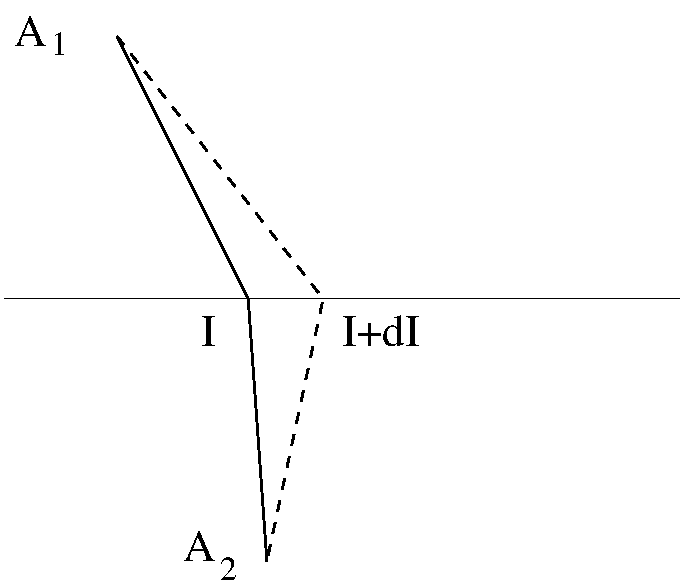
\epsfig{file={../fig/fermat}}}   
 \caption{Snell-Descartes laws can be deduced from fermat principle.}
 \label{figfermat}
\end{figure}
From Fermat principle, $dL=0$.
As $u_1$ is unitary $\vec{u}_1.d\vec{u}_1=0$, and it yields:
\begin{equation}
0=(n_2u_2-n_1u_1).d\vec{I}.
\end{equation}
This last equality is verified by each $d\vec{I}$ belonging to the surface:
\begin{equation}
(n_2\vec{u}_2-n_1\vec{u}_1).\vec t=0
\end{equation}
where $\vec t$ is tangent vector of surface. This is Snell-Descartes equation.
\end{rem}
Another equation of geometrical optics is ikonal equation.
\index{ikonal equation} 
\begin{thm}
Ikonal equation
\begin{equation}
n\frac{dr}{ds}=\mbox{ grad } L
\end{equation}
is equivalent to light ray equation:
\begin{equation}
\frac{d}{ds}(n\frac{dr}{ds})=\mbox{ grad } n
\end{equation}
\end{thm}
\begin{pf}
Let us differentiate ikonal equation with respect to $s$ (see
\cite{ph:optic:Born65}): 
\begin{eqnarray}
\frac{d}{ds}(n\frac{dr}{ds})&=&\frac{d}{ds} \mbox{ grad } L\\
&=&\frac{dr}{ds} \mbox{ grad }(\mbox{ grad } L)\\
&=&\frac{1}{n} \mbox{ grad } L  \mbox{ grad }(\mbox{ grad } L)\\
&=&\frac{1}{2n} \mbox{ grad } n^2
\end{eqnarray}
So:
\begin{equation}
\frac{d}{ds}(n\frac{dr}{ds})=\mbox{ grad } n
\end{equation}
This is light ray equation.
\end{pf}
Fermat principle is so a consequence of Maxwell equations.

\subsection{Physical optics, Diffraction}\label{secdiffra}
%%%%%%%%%%%%%%%%%%%%%%
\subsubsection{Problem position}
%%%%%%%%
Consider a screen $S_1$ with a hole\index{diffraction} 
 $\Sigma$ inside it. Complementar of $\Sigma$ in $S_1$ is noted
$\Sigma^c$ (see figure \ref{figecran}).
\begin{figure}[htb]
 \centerline{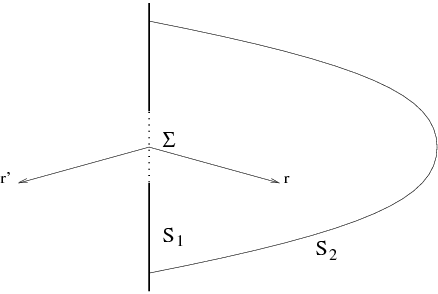
\epsfig{file={../fig/ecran}}}   
 \caption{Names of the various surfaces for the considered diffraction
   problem.} 
 \label{figecran}
\end{figure}
The Electromagnetic signal that falls on $\Sigma$ is assumed not to be
perturbed by the screen $S_c$: value of each component $U$ of the
electromagnetic field is the value $U_{free}$ of $U$ without any screen. The
value of $U$ on the right hand side of $S_c$ is assumed to be zero. Let us
state the diffraction problem \cite{ph:optic:Goodman68} (Rayleigh Sommerfeld
diffraction problem): 
\begin{prob}
Given a function $U_{free}$, find a function $U$ such that:
\begin{equation}
 (\Delta +k^2)U=0\mbox{ in  }\Omega
\end{equation}
\begin{equation}
U=U_{free} \mbox{ on  }\Sigma
\end{equation}
\begin{equation}
U=0\mbox{ on  }\Sigma^c
\end{equation}
\end{prob}
Elementary solution of Helmholtz operator $\Delta +k^2$ in $R^3$ is
\begin{equation}
G_M(M')=\frac{e^{jkr}}{4\pi r}
\end{equation}
where $r=|MM'|$.
Green solution for our screen problem is obtained using images
method\index{images method} (see
section \ref{secimage}). It is solution of following problem:
\begin{prob}
Find  $u$ such that:
\begin{equation}
 (\Delta +k^2)U=\delta_M\mbox{ in  }\Omega
\end{equation}
\begin{equation}
U=0\mbox{ on  }S_1=\Sigma^c\cup\Sigma^c
\end{equation}
\end{prob}
This solution is:
\begin{equation}\label{eqgreendif}
G_M(M')=\frac{1}{4\pi}(\frac{e^{jkr}}{r}+\frac{e^{jkr^s}}{r^s})
\end{equation}
with $r_s=|M_sM'|$ where $M_s$ is the symmetrical of $M$ with respect to the
screen. Thus:
\begin{equation}
U(M)=\int_\Omega u(M')\delta_M(M') dM'=\int_\Omega
u(M')(\Delta+k^2)G_M(M')dM' 
\end{equation}
Now using the fact that in $\Omega$, $\Delta U=-k^2U$:
\begin{equation}
\int_{\Omega}U(M')(\Delta+k^2)G_M(M') dM'=\int_{\Omega}(U(M')\Delta
G_M(M')-G_M(M')\Delta U(M')) dM'.
\end{equation}
Applying Green's theorem, volume integral can be transformed to a surface
integral:
\begin{equation}
\int_{\Omega}(U\Delta G_M-G_M\Delta U) dM'=\int_{\cal S}(U\frac{\partial
 G_M}{\partial n}-G_M\frac{\partial U}{\partial n}) ds'
\end{equation}
where $n$ is directed outwards surface ${\cal S}$.
Integral over $S=S_1+S_2$ is reduced to an integral over
$S_1$  if the {\it Sommerfeld radiation condition}
\index{Sommerfeld radiation condition} is verified:
\subsubsection{Sommerfeld radiation condition}
%%%%%%%%%%%%%%%%%%%%%%%%%%%%%%%%%%%%%%
Consider the particular case where surface $S_2$ is the portion of sphere
centred en P with radius $R$. Let us look for a condition for the integral $I$
defined by:
\begin{equation}
I=\int_{S_2}(U\frac{\partial G}{\partial n}-G\frac{\partial
U}{\partial n}) ds'
\end{equation}
tends to zero when $R$ tends to infinity. We have:
\begin{equation}
\frac{\partial G}{\partial n}=(jk-\frac{1}{R})\frac{e^{jkR}}{R}\sim jkG,
\end{equation}
thus
\begin{equation}
I=\int_{\omega}\frac{e^{jkR}}{R}(\frac{\partial U}{\partial n}-jkU)R^2
d\omega
\end{equation}
where $\omega$ is the solid angle. If, in all directions, condition:
\begin{equation}
\lim_{R\rightarrow\infty}R(\frac{\partial U}{\partial n}-jkU)=0
\end{equation}
is satisfied, then $I$ is zero.
\begin{rem}
If $U$ is a superposition of spherical waves, this condition is
verified\footnote{%%%%% 
Indeed if $U$ is:
\begin{equation}
U=\frac{e^{jkR}}{R}
\end{equation}
then
\begin{equation}
R(\frac{\partial U}{\partial n}-jkU)=-\frac{e^{jkR}}{R}
\end{equation}
tends to zero when $R$ tends to infinity.
}.
\end{rem}

\subsubsection{Huyghens principle}\label{secHuyghens}
%%%%%%%%%%%%%%%%%%%%%%%%
From equation \ref{eqgreendif}, $G$ is zero on $S_1$.
\index{Huyghens principle}
We thus have:
\begin{equation}
U(M)=\frac{1}{4\pi}\int_{S_1}U(M')\frac{\partial G_M(M')}{\partial n}ds'
\end{equation}
Now:
\begin{eqnarray}
\frac{\partial G}{\partial n}&=&\cos
(n,r_{01})(jk-\frac{1}{r_{01}})\frac{e^{jkr_{01}}}{r_{01}}\\
&&-\cos(n,r'_{01})(jk-\frac{1}{r'_{01}})\frac{e^{jkr'_{01}}}{r'_{01}}
\end{eqnarray}
where $r_{01}=MM'$ and $r'_{01}=M_sM'$, $M'$ belonging to $\Sigma$ and
$M_s$ being the symmetrical point of the point $M$ where field $U$ is
evaluated with respect to the screen. Thus:
\begin{equation}
r_{01}=r'_{01}
\end{equation}
and
\begin{equation}
\cos(n,r'_{01})=-\cos(n,r_{01})
\end{equation}
One can evaluate:
\begin{equation}
\frac{\partial G_M}{\partial n}=
2\cos(n,r_{01})(jk-\frac{1}{r_{01}})\frac{e^{jkr_{01}}}{r_{01}}
\end{equation}
For $r_{01}$ large, it yields\footnote{Introducing the wave lenght
$\lambda$ defined by:
\begin{equation}
k=\frac{2\pi}{\lambda}
\end{equation}
}:
\begin{equation}
U(M)=\int_{S_1}U(M')\frac{j}{\lambda}\cos(n,r_{01})
\frac{e^{jkr_{01}}}{r_{01}}ds' 
\end{equation}
This is the {\bf Huyghens principle} :
\begin{prin}
\begin{itemize}
\item Light propagates from close to close. Each surface element reached by it
  behaves like a secondary source that emits spherical wavelet with amplitude
  proportional to the element surface.
\item Complex amplitude of light vibration in one point is the sum of complex
  amplitudes produced by all secondary sources. It is said that vibrations
  interfere to create the vibration at considered point.
\end{itemize}
\end{prin}

Let $O$ a point on $S_1$.
Fraunhoffer approximation \index{Fraunhoffer approximation}  consists in
approximating:  
\begin{equation}
\frac{e^{jkr_{01}}}{r_{01}}
\end{equation}
by
\begin{equation}
\frac{e^{jkR}}{R}e^{jk\vec R_M.\vec R_m /R}.
\end{equation}
where  $R=OM$, $R_m=OM'$, $R_M=OM$.
Then amplitude Fourier transform\index{Fourier transform} of light on
$S_1$ is observed at $M$.







\section{Electromagnetic interaction}
%%%%%%%%%%%%%%%%%%%%%%%%%%%%%%%%%%%%%%
\subsection{Electromagnetic forces}
%%%%%%%%%%%%%%%
Postulates of electromagnetism have to be completed by another postulate that
deals with interactions:
\begin{postulat}
In the case of a charged particle of charge $q$, Electromagnetic force
applied to this particle is:
\begin{equation}
f=qE+qv\wedge B
\end{equation}
where $qE$ is the electrical force (or Coulomb force)
\index{Coulomb force} and $qv\wedge B$ is the Lorentz force.
\index{Lorentz force}
\end{postulat}
This result can be generalized to continuous media using Poynting
vector.\index{Poynting vector} 
\subsection{Electromagnetic energy, Poynting vector}\label{secenergemag}
%%%%%%%%%%%%%%
Previous postulate using forces can be replaced by a ``dual'' postulate that
uses energies:
\begin{postulat}
Consider a volume $V$. The vector $P=E\wedge H$ is called Poynting vector. It
is postulated that flux of vector $P$ trough surface $S$ delimiting volume
$V$, oriented by a entering normal is equal to the Electromagnetic power ${\cal
P}$ given to this volume. 
\end{postulat}
Using Green's theorem, ${\cal P}$ can be written as:
\begin{equation}
{\cal P}=\int\!\!\!\int E\wedge H n ds =-\int\!\!\!\int\!\!\!\int \mbox{ div } (E\wedge H)d\tau
\end{equation}
which yields, using Maxwell equations to:
\begin{equation}
{\cal P}=\int\!\!\!\int\!\!\!\int H\frac{\partial B}{\partial t}+E.j+E\frac{\partial
D}{\partial t}d\tau
\end{equation}
Two last postulates are closely related. In fact we will show now that they
basically say the same thing (even if Poynting vector form can be seen a bit
more general).

Consider a point charge $q$ in a field $E$. Let us move this charge of
$dr$. Previous postulated states that to this displacement corresponds a
variation of internal energy:
\begin{equation}
\delta U=\int E\delta D d\tau
\end{equation}
where $dD$ is the variation of $D$ induced by the charge displacement.
\begin{thm}
Internal energy variation is:
\begin{equation}
\delta U=-f \delta r
\end{equation}
where $f$ is the electrical force applied to the charge.
\end{thm}
\begin{pf}
In the static case, $E$ field has conservative circulation ($\mbox{ rot }
E=0$) so it derives from a potential.
\medskip
Let us write energy conservation equation:
\begin{equation}
\delta U=\int E\delta D  d\tau
\end{equation}
\begin{equation}
\delta U=\int- \mbox{ grad } (V) \delta D  d\tau
\end{equation}
\begin{equation}
\delta U=\int V \mbox{ div }(\delta D)  d\tau-\int \mbox{ div }(V\delta D)  d\tau
\end{equation}
Flow associated to divergence of $V\delta D$ is zero in all the space, indeed
$D$ decreases as $1/r^2$ and $V$ as $1/r$ and surface increases as $r^2$. So:
\begin{equation}
\delta U=\int V \delta \rho  d\tau
\end{equation}
Let us move charge of $\delta r$. Charge distribution goes from $q\delta(r)$
to $q\delta(r+dr)$ where 
$\delta(r)$ is Dirac distribution. We thus have $d
\rho(r)=q(\delta(r+\delta r)-\delta(r))$. So:
,\begin{equation}
\delta U=\int\!\!\!\int\!\!\!\int qV(r)(\delta(r+\delta r)-\delta(r))  d\tau
\end{equation}
thus
\begin{equation}
\delta U=qV(r+\delta r)-qV(r)
\end{equation}
\begin{equation}
\delta U=\mbox{ grad }(qV)\delta r
\end{equation}
Variation is finally $\delta U=-fdr$. Moreover, we prooved that:
\begin{equation}
f=-\mbox{ grad }(qV)=qE
\end{equation}    
\end{pf}


\section{Exercises}
%%%%%%%%%%%%%%%%%%%%%

\begin{exo}\label{exoeqhelmoltz}
Assume constitutive relations to be:
\begin{equation}
D(r,t)=\epsilon(r,t) * E(r,t)
\end{equation}
where $*$ represents temporal convolution\index{convolution} (value of
$D(r,t)$ field at time $t$ S
depends on values of $E$ at preceeding times) and
\begin{equation}
H=\frac{B}{\mu_0}
\end{equation}
Show that in harmonical regime ($E(r,t)={\cal E}(r)e^{i\omega t}$) and without
any charges ${\cal E}(r)$ field verifies {\bf Helmholtz equation}:
\begin{equation}
\Delta {\cal E}+k^{2}{\cal E}=0.
\end{equation}
Give the expression of $k^{2}$.
\end{exo}

\begin{exo}
Show (see \cite{ma:distr:Schwartz65,ma:distr:Zemanian87}) that function $V_{e(r)}$: 
\begin{equation}
V_e(r)=\frac{1}{4\pi\epsilon_0 r}
\end{equation}
is solution of
Maxwell--Gauss equation, {\it i. e } it verifies:
\begin{equation}
\Delta V_e=\frac{\delta}{\epsilon_0}
\end{equation}
\end{exo}

\begin{exo}
Proove charge conservation equation \ref{eqconsdelacharge} from Maxwell
equations. 
\end{exo}

\begin{exo}
Give the expression of electrical potential created by quadripole $Q_{ij}$.
\end{exo}

\begin{exo}
Show from the expression of magnetic energy that force acting on a point
charge $q$ with velocity $v$ is:
\begin{equation}
f=qv\wedge B
\end{equation}

\end{exo}

\chapter{Quantum mechanics}\label{chapmq}
%%%%%%%%%%%%%%%%%

\section{Introduction}
%%%%%%%%%%%%%%%%%%%
In the current state of scientific knowledge, quantum mechanics is the theory
used to describe phenomena that occur at very small scale\footnote{%%%%%%%%
The way that quantum mechanics has been obtained is very different
from the way other theories, relativity for instance, have been
obtained. Relativity therory is based on geometric and invariance
principles. Quantum mechanics is based on observation (operators are
called observables).

Gravitational interaction is difficult to describe with the quantum
mechanics tools. Einstein, even if he played an important role in the
construct of quantum mechanics, was unsatisfied by this theory. His
famous ``God doesn't play dices'' summerizes his point of
view. Electromagnetic interaction can be described using 
quantum dynamics: this is the object of quantum electrodynamics
(QED). This will not presented in this book, so the reader should
refer to specialized books, for instance \cite{ph:mecaq:Cohen87}. 
}%%%%%%%%%%%%%%%%%%%%
(atomic or subatomic). 
The goal of this chapter is to present the mathematical formalism of quantum
mechanics. Applications of quantum mechanics will be seen at chapter
\ref{chapproncorps}. Quantum physics relies on a sequence of postulates that
we present now. The reader is invited to refer to
\cite{ph:mecaq:Cohen73,ph:mecaq:Bohm93} for physical justifications.

\section{Postulates}
%%%%%%%%%%%%%%%%%%%%%%%%%%%%%%

\subsection{State space}\label{secespetat}
%%%%%%%%%
The first postulate deals with the description of the state of a system.
\begin{postulat}
(Description of the state of a system) To each physical system corresponds a
complex 
Hilbert space
${\cal H}$ with enumerable basis.
\end{postulat}
The space ${\cal H}$ have to be precised for each physical system considered. 
\begin{exmp}
For a system with one particle with spin zero in a non relativistic
framework, the adopted state space ${\cal H}$ is $L^2(R^3)$. It is the space
of complex functions of squared summable (relatively to Lebesgue measure)
equipped by scalar product:
\begin{equation}
<\phi|\psi>=\int \phi(x)\bar\psi(x) dx
\end{equation}
This space is called space of orbital states.\index{state space} 
\end{exmp}
Quantum mechanics substitutes thus to the classical notion of position and
speed a function $\psi(x)$ of squared summable. A element $\psi(x)$ of $\cal
H$ is noted $|\psi>$ using Dirac notations.
\begin{exmp}
For a system constituted by a particle with non zero spin
\index{spin}$s$, in a non relativistic framework, state space is the tensorial
product $L^2(R^3)\otimes C^n$ where $n=2s+1$.
Particles with entire spin are called bosons;\index{bosons} Particles with
semi-entire spin are called fermions.\index{fermions} 
\end{exmp}
\begin{exmp}
For a system constituted by $N$ distinct particles, state space is the
tensorial product of Hilbert spaces $h_i$ ($i
\in (1,\dots,N)$)
where $h_i$ is the state space associated to particle $i$.
\end{exmp}
\begin{exmp}\label{exmppauli}
For a system constituted by $N$ identical particles, the state space is a
subspace of $\otimes_{i=1}^N h_i$ where $h_i$ is the state space associated to
particle $i$.
Let $\psi_{\alpha_1,\dots,\alpha_N}$ be a function of this subspace. It can be
written:
\begin{equation}
\psi_{\alpha_1,\dots,\alpha_N} = \phi_{\alpha_1}(1)\otimes \dots
\otimes\phi_{\alpha_2}(N) 
\end{equation}
where $\phi_{\alpha_i}\in h_i$.
Let $P^{\pi}$ be the operator permutation \index{permutation} from
$\otimes_{i=1}^N h_i$ into
$\otimes_{i=1}^N h_i$ defined by:
\begin{equation}
P^{\pi}(\psi_{\alpha_1,\dots,\alpha_N})=
\phi_{\alpha_1}(\pi(1))\otimes \dots 
\otimes\phi_{\alpha_2}(\pi(N)) 
\end{equation}
where $\pi$ is a permutation of $(1,\dots,N)$.
A vector is called symmetrical if it can be written:
\begin{equation}
\phi^s=\frac{1}{k^s}\sum_\pi P^\pi(\psi_{\alpha_1,\dots,\alpha_N})
\end{equation}
A vector is called anti-symetrical if it can be written:
\begin{equation}
\phi^a=\frac{1}{k^a}\sum_\pi (-1)^{p_\pi}
P^\pi(\psi_{\alpha_1,\dots,\alpha_N}) 
\end{equation}
where $(-1)^{p_\pi}$ is the signature \index{signature} (or parity) of the
permutation $\pi$, $p_\pi$ being the number of
transpositions whose permutation $\pi$ is product.
Coefficients $k^s$ and $k^a$ allow to normalize wave functions. Sum is
extended to all permutations $\pi$ of $(1,\dots,N)$.
Depending on the particle, symmetrical or anti-symetrical vectors should be
chosen as state vectors. More precisely:
\begin{itemize}
\item For bosons, state space is the subspace of $\otimes_{i=1}^N h_i$ made by
  symmetrical vectors.
\item For fermions, state space is the subspace of $\otimes_{i=1}^N h_i$ made
  by anti-symetrical vectors.
\end{itemize}
\end{exmp}
To present the next quantum mechanics postulates,
``representations'' \cite{ma:equad:Dautray5,ph:mecaq:Cohen73} have to be
defined. 
\subsection{Schr\"odinger representation}
%%%%%%
Here is the statement of the four next postulate of quantum mechanics in
Schr\"odinger representation.\index{Schr\"odinger representation}
\begin{postulat}
(Description of physical quantities) Each measurable physical quantity $\cal
A$ can be described by an operator $A$ acting in $\cal H$. This operator is an
observable.
\end{postulat}
\begin{postulat}
(Possible results)
The result of a measurement of a physical quantity $\cal A$ can be only one of
the eigenvalues of the associated observable $A$.
\end{postulat}
\begin{postulat}(Spectral decomposition principle)
When a physical quantity $\cal A$ is measured in a system which is in state
normed $|\psi \mathrel{>} $ , the average value of measurement is $<A>$ :
\begin{equation}
<A>=<\psi|A\psi>
\end{equation}
where $< . | . >$ represents the scalar product in $\cal H$.
In particular, if $A=\sum |v_i>a_i<v_i|$, probability to obtain the value
$a_i$ when doing a measurement is:
\begin{equation}
P(a_i)=<\psi|v_i><v_i|\psi>
\end{equation}
\end{postulat}
\begin{postulat}
(Evolution)
The evolution of a state vector $\psi(t)$ obeys the
Schr\"odinger\footnote{The Autria physicist Schr\"odinger first
proposed this equation in 1926 as he was working in Zurich. He
received the Nobel price in 1933 with Paul Dirac for their work in
atomic physics.} equation:
\begin{equation}
i\hbar \frac{d}{dt} |\psi(t)\mathrel{>} =H(t)|\psi(t)\mathrel{>} 
\end{equation}
where $H(t)$ is the observable associated to the system's energy.
\end{postulat}
\begin{rem}
State a time $t$ can be expressed as a function of state a time $0$:
\begin{equation}
|\psi(t)\mathrel{>}=U|\psi(0)\mathrel{>}
\end{equation}
Operator $U$ is called evolution 
operator.\index{evolution operator} 
It can be shown that $U$ is unitary.\index{unitary operator}
\end{rem}
\begin{rem}
When operator $H$ doesn't depend on time, evolution equation can be easily
integrated and it yields:
\begin{equation}
|\psi(t)\mathrel{>}=U|\psi(0)\mathrel{>}
\end{equation}
with
\begin{equation}
U=e^{-iHt/\hbar}
\end{equation}
When $H$ depends on time, solution of evolution equation 
\begin{equation}
i\hbar \frac{\partial U(t)}{\partial t}=H(t)U(t)
\end{equation}
is {\bf not}:
\begin{equation}
U(t)=e^{\frac{i}{\hbar}\int_0^t H(t')dt'}
\end{equation}
\end{rem}
\subsection{Other representations}\label{secautresrep}
%%%%%%%%%%%%%%%%%%%%%%%
Other representations can be obtained by unitary transformations.
\begin{defn}
By definition\cite{ph:mecaq:Cohen73}, an operator $U$ is unitary if its inverse
$U^{-1}$ is equal to the adjoint operator $U^+$ of $U$:
\begin{equation}
U^+U=UU^+=1
\end{equation}
\end{defn}
\begin{prop}
If $A$ is hermitic, then operator $T=e^{iA}$ is unitary.
\end{prop}
Indeed:
\begin{equation}
T^+=e^{-iA^+}=e^{-iA}
\end{equation}
\begin{equation}
T^+T=e^{-iA}e^{+iA}=1
\end{equation}
\begin{equation}
TT^+=e^{iA}e^{-iA}=1
\end{equation}
\begin{prop}
Unitary transformations conserve the scalar product.
\end{prop}
\begin{pf} Indeed, if
\begin{equation}
\tilde{\psi_1}=U\psi_1 \mbox{ et  } \tilde{\psi_2}=U\psi_2
\end{equation}
then
\begin{equation}
 \mathrel{<} \psi_1|\psi_2\mathrel{>} = \mathrel{<} \tilde{\psi_1}|\tilde{\psi_2}\mathrel{>} 
\end{equation} 
\end{pf}
\subsection{Heisenberg representation}
%%%%%%%%%%%%%%%%%%%%%%%%%%%%%%
We have seen that evolution operator provides state at time $t$ as a function
of state at time $0$:
\begin{equation}
\phi(t)=U\phi(0)
\end{equation}
Let us write $\phi_S$ the state in Schr\"odinger representation and
$\phi_H$ the state in Heisenberg representation.
\index{Heisenberg representation}
Heisenberg\footnote{Wener Heisenberg received the Physics Nobel price
for his work in quatum mechanics}%%%%%%%%%
representation is defined from Schr\"odinger representation by the
following unitary transformation:
\begin{equation}
\phi_H=V\phi_S
\end{equation}
with
\begin{equation}
V=U^{-1}
\end{equation}
In other words, state in Heisenberg representation is characterized  by a wave
function independent on $t$ and equal to the corresponding state in
Schr\"odinger representation for 
$t=0$ : $\phi_H=\phi_S(0)$.
This allows us to adapt the postulate to Heisenberg representation:
\begin{postulat}(Description of physical quantities)
To each physical quantity and corresponding state space ${\cal H}$ can be
associated a function $t\in R\rightarrow A_H(t)$ with self adjoint operators
$A_H(t)$ in ${\cal H}$ values.
\end{postulat}
Note that if $A_S$ is the operator associated to a physical quantity
$\cal A$ in Schr\"odinger representation, then the relation between $A_S$
and $A_H$ is:
\begin{equation}
A_H(t)=U^+A_SU
\end{equation}
Operator $A_H$ depends on time, even if $A_S$ does not.
\begin{postulat}(Possible results)
Value of a physical quantity at time $t$ can only be one of the points of the
spectrum of the associated self adjoint operator $A(t)$.
\end{postulat}
Spectral decomposition principle stays unchanged:
\begin{postulat}(Spectral decomposition principle)
When measuring some physical quantity $\cal A$ on a system in a normed state
$|\psi_H \mathrel{>} $, the average value of measurements is $<A_H>$ :
\begin{equation}
<A>=<\psi_H|A_H\psi_H>
\end{equation}
\end{postulat}
The relation with Schr\"odinger is described by the following equality:
\begin{equation}
<\psi_H|A_H\psi_H>=<\psi_SU|U^+A_SU|U^+\psi_H>
\end{equation}
As $U$ is unitary:
\begin{equation}
<\psi_H|A_H\psi_H>=<\psi_S|A_S\psi_S>
\end{equation}
Postulate on the probability to obtain a value to measurement remains
unchanged, except that operator now depends on time, and vector doesn't.
\begin{postulat}(Evolution)
Evolution equation is (in the case of an isolated system):
\begin{equation}
i\hbar \frac{dA}{dt}(t)=-(HA(t)-A(t)H)=-[H,A(t)]
\end{equation}
\end{postulat}
This equation is called Heisenberg equation for the observable.
\begin{rem}
If system is conservative ($H$ doesn't depend on time), then we have seen that
\begin{equation}
U=e^{-iHt/\hbar}.
\end{equation}
if we associate to a physical quantity at time $t=0$
operator $A(0)=A$ identical to operator associated to this quantity in
Schr\"odinger representation, operator
$A(t)$ is written:
\begin{equation}
A(t)=e^{+i\frac{Ht}{\hbar}}A e^{-i\frac{Ht}{\hbar}}
\end{equation}
\end{rem}
\subsection{Interaction representation}
%%%%%%%%%%%%%%%%%%%%%%%
Assume that hamiltonian $H$ can be shared into two parts $H_0$ and
$H_i$. In particle, $H_i$ is often considered as a perturbation of $H_0$ and
represents interaction between unperturbed states (eigenvectors of $H_0$).
Let us note $|\psi_S\mathrel{>} $ a state in Schr\"odinger representation and 
$|{\psi}_I\mathrel{>} $ a state in interaction 
representation.\index{interaction representation}
\begin{equation}
|{\psi}_I\mathrel{>} =U_0|\psi_S\mathrel{>}
\end{equation}
with 
\begin{equation}
U_0=e^{iH_0t/\hbar}
\end{equation}
\begin{postulat}(Description of physical quantities)
To each physical quantity in a state space
${\cal H}$ is associated a function $t\in R\rightarrow A_I(t)$ with self
adjoint operators $A_I(t)$ in ${\cal H}$ values.
\end{postulat}
If $A_S$ is the operator associated to a physical quantity 
$\cal A$ in Schr\"odinger representation, then relation between $A_S$ and $A_I$ is:
\begin{equation}
A_I(t)=U_0A_SU_0^+=e^{iH_0t/\hbar}A_S e^{-iH_0t/\hbar}
\end{equation}
So, $A_I$ depends on time, even if $A_S$ does not.
Possible results postulate remains unchanged.
\begin{postulat}
When measuring a physical quantity $\cal A$ for a system in state $\psi_I$,
the average value of $A_I$ is:
\begin{equation}
<\psi_I|A_I\psi_I>
\end{equation}
\end{postulat}
As done for Heisenberg representation, one can show that this result is
equivalent to the result obtained in the
Schr\"odinger representation. From Schr\"odinger equation, evolution equation
for interaction representation can be obtained immediately:
\begin{postulat}(Evolution)
Evolution of a vector $\psi_I$ is given by:
\begin{equation}
i\hbar \frac{d}{dt} |\psi_I(t)\mathrel{>}
= V_I|\psi_I(t)\mathrel{>}  
\end{equation}
with
\begin{equation}
V_I=e^{iH_0t/\hbar}H_ie^{-iH_0t/\hbar}
\end{equation}
\end{postulat}
Interaction representation makes easy perturbative calculations. It is used in
quantum electrodynamics\cite{ph:mecaq:Cohen88}.
In the rest of this book, only Schr\"odinge representation will be used.
\section{Some  observables}
%%%%%%%%%%%%%%%%
\subsection{Hamiltonian operators}
%%%%%%%%%%%%%%%%%%%%%%%%%%%%%%%%
Hamiltonian operator \index{hamiltonian operator} has been introduced as
the infinitesimal generator times  $i\hbar$ of the evolution
group. Experience, passage methods from classical mechanics to quantum mechanics
allow to give its expression for each considered system.
Schr\"odinger equation rotation invariance implies that the hamiltonian is a
scalar operator
(see appendix \ref{chapgroupes}).
\begin{exmp}
Classical energy of a free particle is
\begin{equation}
E_c=\frac{p^2}{2m}.
\end{equation}
Its quantum equivalent, the hamiltonian $H$ is:
\begin{equation}
H=\frac{P^2}{2m}.
\end{equation}
\end{exmp}
\begin{rem}{\bf Passage relations}
Quantification rules \cite{ph:mecaq:Cohen73} indicate how for a physical
quantity ${\cal A}$ already defined in classical mechanics, the operator $A$
of quantum mechanics has to be defined. In a general way, observable
$A$ associated to physical quantity $\cal A$ 
defined classically is obtained by replacing in suitably
symmetrised\footnote{Indeed, in general the product of two operators
does not commute, on the contrary of the scalar product of two vectors
or the product of two scalars. For instance the classical quantity 
\begin{equation}
{\cal A}=p.r
\end{equation}
where $p$ is the classical momentum and $r$ the classical position
have the equivalent:
\begin{equation}
A=\frac{1}{2}[P.R+R.P]
\end{equation}
where $P$ is the momentum observable, and $R$ the position observable,
observables that are introduced in the next part of the present section.
For any operator $A$ and $B$, the quantity
\begin{equation}
[A,B]=AB-BA
\end{equation}
is called the {\bf commutator}\index{commutator} of $A$ and $B$ and is
in genral 
different from zero.
}
 expression
of $\cal A$, r and p by observables $R$ and $P$. 
\end{rem}
\subsection{Position operator}
%%%%%%%%%%%%%%%%%%%%%%%%%%
Classical notion of position $r$ of a particle leads to associate to a
particle a set of three operators (or observables)
$R_x,R_y,R_z$ called position operators\index{position operator} and
defined by their action on a function $\phi$ of the orbital Hilbert space:
\begin{equation}
R_x\phi(x,y,z)=x\phi(x,y,z)
\end{equation}

\begin{equation}
R_y\phi(x,y,z)=y\phi(x,y,z)
\end{equation}

\begin{equation}
R_z\phi(x,y,z)=z\phi(x,y,z)
\end{equation}

\subsection{Momentum operator}
%%%%%%%%%%%%%%%%%%%%%%%%%%%%%%%
In the same way, to ``classical'' momentum of a particle is
associated a set of three observables $P=(P_x,P_y,P_z)$. Action of operator
$P_x$ is defined by \index{momentum operator}:
\begin{equation}\label{eqdefmomP}
P_x\phi=\frac{\hbar}{i}\frac{\partial}{\partial x} \phi
\end{equation}
Operators $R$ and $P$ verify commutation relations called
{\bf canonical commutation relations}\index{commutation relations} :
\begin{equation}
[R_i,R_j]=0
\end{equation}
\begin{equation}
[P_i,P_j]=0
\end{equation}
\begin{equation}
[R_i,P_j]=i\hbar \delta_{ij}
\end{equation}
where $\delta_{ij}$ is Kronecker symbol (see appendix
\ref{secformultens}) and where for any operator $A$ and $B$,
$[A,B]=AB-BA$. Operator $[A,B]$ is called the {\bf commutator} of $A$
and $B$.
\subsection{Kinetic momentum operator}
%%%%%%%%%%%%%%%%%%%%%%%%%%%%%
\begin{defn}
A kinetic momentum 
\index{kinetic moment operator}
$J$, is a set of three operators
$J_x,J_y,J_z$ that verify following commutation relations
\index{commutation relations}:
\begin{equation}
[J_i,J_l]=i\hbar\epsilon_{kil}J_k
\end{equation}
that is:
\begin{equation}
[J_x,J_y]=i\hbar J_z
\end{equation}
\begin{equation}
[J_y,J_z]=i\hbar J_x
\end{equation}
\begin{equation}
[J_z,J_x]=i\hbar J_y
\end{equation}
where $\epsilon_{ijk}$ is the permutation signature tensor (see appendix
\ref{secformultens}). Operator $J$ is called a vector operator (see
appendix \ref{chapgroupes}.
\end{defn}
\begin{exmp}
{\bf Orbital kinetic momentum}
\begin{thm}
Operator defined by $L_i=\epsilon_{ijk}R_jP_k$ is a kinetic momentum. It is
called orbital kinetic momentum.
\end{thm}
\begin{pf}
Let us evaluate (see \cite{ph:mecaq:Bohm93}) commutator:
\begin{eqnarray}
[L_i,L_l]&=&\epsilon_{ijk}\epsilon_{lmn}(x_jp_kx_mp_n-x_mp_nx_jp_k)\\
&=&i\hbar
\epsilon_{ijk}\epsilon_{lmn}(\delta_{km}x_jp_n-\delta_{nj}x_mp_k)\\ 
&=&i\hbar \epsilon_{ijk}\epsilon_{lkn}x_jp_n -
\epsilon_{ijk}\epsilon_{lmj}x_mp_k 
\end{eqnarray}
where canonical commutation relations have been used. Changing notations:
\begin{eqnarray}
[L_i,L_l]&=&i\hbar \epsilon_{imk}\epsilon_{lkn}x_mp_n -
\epsilon_{ijn}\epsilon_{lmj}x_mp_n\\
&=&i\hbar x_mp_n(\delta_{in}\delta_{ml}-\delta_{nl}\delta_{im})\\
&=&i\hbar x_mp_n\epsilon_{ikl}\epsilon_{knm}
\end{eqnarray}
\end{pf}
\begin{postulat}
To orbital kinetic momentum is associated a magnetic moment $M$:
\begin{equation}
M=\frac{\mu_B}{\hbar}L
\end{equation}
\end{postulat}
\end{exmp}
\begin{exmp}
{\bf Postulates for the electron.}
We have seen at section \ref{secespetat} that state space for an electron (a
fermion of spin $s=1/2$) is
the tensorial product orbital state space and spin state space. One defines an
operator $S$ called spin operator that acts inside spin state space. It is
postulated that this operator is a kinetic momentum and that it appears in the
hamiltonian {\it via} a magnetic momentum.
\begin{postulat}
Operator $S$ is a kinetic moment.
\end{postulat}
\begin{postulat}
Electron is a particle of spin $s=1/2$ and it has an intrinsic magnetic moment
\index{magnetic moment}: 
\begin{equation}
M_S=2\frac{\mu_b}{\hbar}S
\end{equation}
\end{postulat}
\end{exmp}


\section{Linear response in quantum mechanics}\label{secreplinmq}
%%%%%%%%%%%%%%%%%%%%%%%%%%%%%%%%%%
Let $ \mathrel{<} A\mathrel{>} (t)$ be the average of operator (observable) $A$. This
average is accessible to the experimentator (see
\cite{ph:mecaq:Cohen73}).
The case where $H(t)$ is proportional to $sin(\omega t)$ is treated in
\cite{ph:mecaq:Cohen73} 
Case where $H(t)$ is proportional to  $\delta(t)$ is treated here.  
Consider following problem:
\begin{prob}
Find $\psi$ such that:
\begin{equation}
i\hbar \frac{d\psi}{dt}=(H_0+W_i(t))\psi
\end{equation}
with
\begin{equation}
W_i(t)=W_i^c.\delta(t)
\end{equation}
and evaluate: 
\begin{equation}
 \mathrel{<} qZ\mathrel{>} = \mathrel{<} \psi|qZ|\psi\mathrel{>} 
\end{equation}
\end{prob}
\begin{rem}
Linear response can be described in the classical frame where Schr\"odinger
equation is replaced by a classical mechanics evolution equation. Such models
exist to describe for instance electric or magnetic susceptibility.
\end{rem}
Using the interaction representation\footnote{%%%%%%
This change of representation is equivalent to a WKB method. Indeed,
$\tilde{\psi(t)}$ becomes a slowly varying function of $t$ since temporal
dependence is absorbed by operator $e^{\frac{iH_0t}{\hbar}}$}%%%%%%%%%%% 
\begin{equation}
\tilde{\psi(t)}=e^{\frac{iH_0t}{\hbar}}\psi(t)
\end{equation}
and
\begin{equation}
\tilde{W}_i(t)=e^{\frac{iH_0t}{\hbar}}W_ie^{\frac{-iH_0t}{\hbar}}
\end{equation}
Quantity $ \mathrel{<} qZ\mathrel{>} $ to be evaluated is:
\begin{equation}
 \mathrel{<} qZ\mathrel{>} = \mathrel{<} \tilde{\psi}|q\tilde{Z}|\tilde{\psi}\mathrel{>} 
\end{equation}
\begin{equation}
i\hbar \frac{d\tilde{\psi}}{dt}=\tilde{W}_i(t)\tilde{\psi}
\end{equation}
At zeroth order:
\begin{equation}
 \frac{d\tilde{\psi}}{dt}=0
\end{equation}
Thus:
\begin{equation}
\tilde{\psi}^0(t)=\tilde{\psi}^0(0)
\end{equation}
Now, $\tilde{\psi}$ has been prepared in the state $\psi_0$, so:
\begin{equation}
\tilde{\psi}^0(t)=\psi_0(t)
\label{pert1}
\end{equation}
At first order:
\begin{equation}
\tilde{\psi}^1(t)=\tilde{\psi}^1(0)+\frac{1}{i\hbar}\int_0^t\tilde{W}_i(t\prime)\tilde{\psi}^0(t\prime)dt\prime
\end{equation}
thus, using properties of $\delta$ Dirac distribution:
\begin{equation}
\tilde{\psi}^1(t)=\frac{1}{i\hbar}W^i_c\psi_0.
\label{pert2}
\end{equation}
Let us now calculate the average:
Up to first order,
\begin{eqnarray}
 \mathrel{<} qZ\mathrel{>} &=& \mathrel{<}
\tilde{\psi}^0+\tilde{\psi^1}|e^{\frac{iH_0t}{\hbar}}
qZe^{\frac{iH_0t}{\hbar}}|\tilde{\psi}^0+\tilde{\psi^1}\mathrel{>} 
\\ 
&=& \mathrel{<} \tilde{\psi}^0|
e^{\frac{iH_0t}{\hbar}}qZe^{\frac{iH_0t}{\hbar}}|\tilde{\psi}^1\mathrel{>}
+ \mathrel{<}
\tilde{\psi}^1|e^{\frac{iH_0t}{\hbar}}
qZe^{\frac{iH_0t}{\hbar}}|\tilde{\psi}^0\mathrel{>} 
\end{eqnarray}
Indeed, $ \mathrel{<} \tilde{\psi}^0|qZ|\tilde{\psi}^0\mathrel{>} $ is zero
because $Z$ is an odd operator.
\begin{eqnarray}
\lefteqn{ \mathrel{<}
\tilde{\psi}^0|e^{\frac{iH_0t}{\hbar}}qZ
e^{\frac{iH_0t}{\hbar}}|\tilde{\psi}^1\mathrel{>} 
=}\\ 
&=& \mathrel{<} {\tilde{\psi}}^0|
e^{\frac{iH_0t}{\hbar}}qZe^{\frac{-iH_0t}{\hbar}}|{\psi}_k\mathrel{>}
\mathrel{<} {\psi}_k|{\tilde{\psi}}^1\mathrel{>}  
\end{eqnarray}
where, closure relation has been used. Using perturbation results given by
equation~\ref{pert1} and equation~\ref{pert2}:
\begin{equation}
 \mathrel{<} \tilde{\psi}^0|qZ|\tilde{\psi}^1\mathrel{>} =e^{i\omega_{0k}t} \mathrel{<} {\psi}^0|qZ|{\psi}^k\mathrel{>} \frac{1}{i\hbar} \mathrel{<} {\psi}^k|W^c_i|{\psi}^0\mathrel{>} 
\end{equation}
We have thus:
\begin{eqnarray}
 \mathrel{<} qZ\mathrel{>} (t)&=& 0 \mbox{ if } t < 0\\
 \mathrel{<} qZ\mathrel{>} (t)&=&
e^{i\omega_{0k}t} \mathrel{<} {\psi}^0|qZ|{\psi}^k\mathrel{>} \frac{1}{i\hbar} \mathrel{<} {\psi}^k|W^c_i|{\psi}^0\mathrel{>} +CC
\mbox{ if not }
\end{eqnarray}
Using Fourier transform\footnote{%%%%%%%%%
Fourier transform of:
\begin{equation}
f(t)=e^{-i\omega_0t}
\end{equation}
and Fourier transform of:
\begin{equation}
g(t)=H(t)e^{-i\omega_0t}
\end{equation}
are different: Fourier transform of $f(t)$ does not exist! (see \cite{ma:distr:Schwartz65,ma:distr:Zemanian87})
}%%%%%%%%%%%%%%%%%%
:
\begin{equation}
\mathrel{<} qZ\mathrel{>} (\omega)=2q^2E\sum_{k\neq 0}\omega_{0k}\frac{| \mathrel{<} \psi_0|Z|\psi_k\mathrel{>} |^2}{\omega_{k0}^2-\omega^2}
\end{equation}


\section{Exercises}
%%%%%%%%%%%%%%%%%%%
\begin{exo}
Study the binding between position operator $R_x$ and momentum operator $P_x$
with the infinitesimal generator of the translation group (see
\cite{ma:equad:Dautray5}). 
\end{exo}

\begin{exo}
Study the connection between kinetic moment operator $L$ and the infinitesimal
generator of the rotations group (see
\cite{ma:equad:Dautray5}.
\end{exo}

\begin{exo}
Study the linear response of a classical oscillator whose equation is:
\begin{equation}
\frac{d^{2}x}{dt^{2}}+\gamma \frac{dx}{dt}+\omega_{0}^{2}x=f(t)
\end{equation}
where $f(t)$ is the excitation.
Compare with the results obtained at section \ref{secreplinmq}.
\end{exo}

\chapter{N body problem in quantum mechanics}\label{chapproncorps} 
%%%%%%%%%%%%%%%%%%%%%%%%%%%%%%%%%%%%%%%
\section{Introduction}
%%%%%%%%%%%%%%%%%%%%%%%
In this chapter, $N$ body problems that quantum mechanics can treat are
presented. In atoms, elements in interaction are the nucleus and the
electrons. In molecules, several nuclei and electrons are in
interaction. Cristals are characterized by a periodical arrangment of
their atoms. In this chapter, only 
spectral properties of hamiltonians are presented. Thermodynamical properties
of collections of atoms and molecules are presented at next chapter.
From a mathematical point of view, this chapter is an application of the
spectral method presented at section \ref{chapmethspec} to study linear
evolution problems.
\section{Atoms}\label{secatomemq}
%%%%%%%%%%%%%%%%%%
\subsection{One nucleus, one electron}\label{sechydrog}
%%%%%%%%%%%%%%%%
This case corresponds to the study of hydrogen atom.\index{atom} It is a
particular case of particle in a central potential problem, so that we apply
methods presented at section~\ref{secpotcent} to treat this
problem. Potential is here:
\begin{equation}\label{eqpotcenhy}
V(r)=-\frac{e}{r^2}
\end{equation}
It can be shown that eigenvalues of hamiltonian $H$ with central potential depend in general on two
quantum numbers $k$ and $l$, but that for particular potential given by
equation \ref{eqpotcenhy}, eigenvalues depend only on sum $n=k+l$.



\subsection{Rotation invariance}\label{secpotcent}
%%%%%%%%%%%%%%%%%%%%%%%%%%%%%%%%%%%%%%%%%%%%%
We treat in this section the particle in a central potential problem
\cite{ph:mecaq:Cohen73,ma:equad:Dautray5,ph:elect:Jackson75}. The spectral
problem to be solved is given by the following equation:
\begin{equation}
-[\frac{\hbar^2}{2\mu}\Delta+V(r)]\phi(r)=E\phi(r).
\end{equation}
Laplacian operator can be expressed as a function of $L^2$ operator.
\begin{thm}
Laplacian operator $\Delta$ can be written as:
\begin{equation}
\Delta=-\frac{1}{r^2}L^2+\frac{\partial^2}{\partial
r^2}+\frac{2}{r}\frac{\partial}{\partial r}
\end{equation}
\end{thm}
\begin{pf}
Here, tensorial notations are used (Einstein convention). By definition:
\begin{equation}
L_i=\epsilon_{ijk}x_jp_k
\end{equation}
So:
\begin{eqnarray}
L_iL_i&=&\epsilon_{ijk}\epsilon_{ilm}x_{j}p_k x_l p_m\\
&=&(\delta_{jl}\delta_{km}-\delta_{jm}\delta{kl})x_{j}p_kx_l p_m\\
&=&x_jx_jp_kp_k-x_jp_kx_kp_j
\end{eqnarray}
The writing order of the operators is very important because operator do not
commute. They obey following commutation relations:
\begin{equation}
[x_i,p_j]=i \hbar \delta_{ij}
\end{equation}
\begin{equation}
[x_j,x_k]=0
\end{equation}
\begin{equation}
[p_j,p_k]=0
\end{equation}
From equation \ref{eqdefmomP}, we have:
\begin{equation}
p_k=-i\hbar \frac{\partial}{\partial x_k}
\end{equation}
thus
\begin{equation}
x_jx_jp_kp_k=-x^2\hbar^2\Delta.
\end{equation}
Now,
\begin{eqnarray}
x_jp_kx_kp_j&=&[i\hbar\delta_{ik}+p_kx_j]x_kp_j\\
&=&i\hbar x_kp_k+p_kx_jx_kp_j\\
&=&i\hbar x_kp_k+p_kx_kx_jp_j
\end{eqnarray}
Introducing operator:
\begin{equation}
\tilde D=x_k\frac{\partial}{\partial x_k}
\end{equation}
we get the relation:
\begin{equation}\label{eql2pri}
L^2=-x^2\Delta+\tilde D^2+\tilde D
\end{equation}
Using spherical coordinates, we get:
\begin{equation}
\tilde D=r\frac{\partial}{\partial r}
\end{equation}
and
\begin{equation}
\tilde D^2=(r\frac{\partial}{\partial r})(r\frac{\partial}{\partial
r})=r^2\frac{\partial^2}{\partial r^2}+\frac{\partial}{\partial r}
\end{equation}
So, equation \ref{eql2pri} becomes:
\begin{equation}
\Delta=-\frac{1}{r^2}L^2+\frac{\partial^2}{\partial
r^2}+\frac{2}{r}\frac{\partial}{\partial r}
\end{equation}
\end{pf}
Let us use the problem's symmetries:
\begin{itemize}
\item Since:
      \begin{itemize}
       \item $L_z$ commutes with operators acting on $r$
       \item $L_z$ commutes with $L^2$
      \end{itemize}
operator $L_z$ commutes with $H$
\item $L^2$ commutes with $H$
\end{itemize}
we look for a function $\phi$ that diagonalizes simultaneously
$H,L^2,L_z$ that is such that: 
\begin{eqnarray}
H\phi(r)&=&E\phi(r)\\
L^2\phi(r)&=&l(l+1)\hbar^2\phi(r)\\
L_z\phi(r)&=&m\hbar\phi(r)
\end{eqnarray}
Spherical harmonics $Y^m_l(\theta,\phi)$ can be introduced now:
\begin{defn}
Spherical harmonics  $Y^m_l(\theta,\phi)$ are eigenfunctions common to
operators $L^2$ and $L_z$. It can be shown that:
\begin{eqnarray}
L^2Y^m_l&=&l(l+1)Y^m_l\\
L_zY^m_l&=&mY^m_l
\end{eqnarray}
\end{defn}
Looking for a solution $\phi(r)$ that can\footnote{Group theory
argument should be used to prove that solution actually are of this
form.}%%%
 be written (variable separation): 
\begin{equation}
\phi(r)=R(r)Y^m_l(\theta,\phi)
\end{equation}
problem becomes one dimensional:
\begin{equation}\label{eqaonedimrr}
-[\frac{\hbar^2}{2\mu}(\frac{d^2}{dr^2}+\frac{2}{r}\frac{\partial}{\partial
r})+\frac{l(l+1)}{2\mu r^2}\hbar^2+V(r)]R_{l}(r)=E_{kl}R_{l}(r)
\end{equation}
where  $R(r)$ is indexed by $l$ only.
Using the following change of variable:
$R_{l}(r)=\frac{1}{r}u_{l}(r)$, one gets the following spectral equation:
\begin{equation}
-[\frac{\hbar^2}{2\mu}\frac{d^2}{dr^2}+V_e(r)]u_{kl}(r)=E_{kl}u_{kl}(r)
\end{equation}
where
\begin{equation}
V_e(r)=\frac{l(l+1)}{2\mu r^2}\hbar^2+V(r)
\end{equation}
The problem is then reduced to the study of
the movement of a particle in an effective potential $V_e(r)$. To go
forward in the solving of this problem, the expression of
potential $V(r)$ is 
needed.  Particular case of hydrogen introduced at section
\ref{sechydrog} corresponds to a potential $V(r)$ proportional to
$1/r$ and leads to an accidental degeneracy.


\subsection{One nucleus, N electrons}
%%%%%%%%%%%%%%%%
This case corresponds to the study of atoms different from hydrogenoids
atoms. The Hamiltonian describing the problem is:
\begin{equation}
H=\sum_i-\frac{\hbar^2}{2m}\Delta_i-
\frac{1}{4\pi\epsilon_0}\frac{Ze^2}{r_i}+ \sum_{j\mathrel{>}
i}\frac{1}{4\pi\epsilon_0}\frac{e^2}{r_{ij}}+T_2 
\end{equation}
where $T_2$ represents a spin-orbit interaction term that will be treated
later. Here are some possible approximations:
\subsubsection{N independent electrons}
%%%%%%%%%%%%%%%%%%%%%%
This approximation consists in considering each electron as moving in a mean
central potential and in neglecting spin--orbit interaction. It is a ``mean
field'' approximation. The electrostatic interaction term
\begin{equation}
-\frac{1}{4\pi\epsilon_0}\frac{Ze^2}{r_i}+\sum_{j\mathrel{>}
i}\frac{1}{4\pi\epsilon_0}\frac{e^2}{r_{ij}}
\end{equation}
is modelized by the sum $\sum W(r_i)$, where $W(r_i)$ is the mean potential
acting on particle $i$. The hamiltonian can thus be written:
\begin{equation}
H_0=\sum_ih_i
\end{equation}
where $h_i=-\frac{\hbar^2}{2m}\Delta_i+W(r_i)$.
\begin{rem}
More precisely, $h_i$ is the linear operator acting in the tensorial
product space $\otimes_{i=1}^N E_i$ and defined by its action on function that are
tensorial products:
\begin{equation}
[1_1\otimes\dots\otimes 1_{i-1}\otimes h_i \otimes 1_{i+1}\dots\otimes
1_{N}] 
(\phi_1\otimes\dots\phi_N)
=h_i(\phi_1)\otimes\dots\phi_N 
\end{equation}
\end{rem}
It is then sufficient to solve the spectral problem in a space
$E_i$ for operator $h_i$. Physical kets are then constructed by
anti symmetrisation (see example \ref{exmppauli} of chapter \ref{chapmq}) in
order to satisfy Pauli principle.\index{Pauli}
The problem is a central potential problem (see section
\ref{secpotcent}). However, potential $W(r_i)$ is not like $1/r$ as in the
hydrogen atom case and thus the accidental degeneracy is not 
observed here. The energy depends on two quantum numbers $l$ (relative
to kinetic 
moment) and $n$ (rising from the radial equation \ref{eqaonedimrr}).
Eigenstates in this approximation are called electronic configurations. 
\begin{exmp}
For the helium atom, the fundamental level corresponds to an electronic
configuration noted $1s^2$. A physical ket is obtained by anti symetrisation of
vector:
\begin{equation}
|1:n,l,m_l,m_s>\otimes|2:n,l,m_l,m_s>
\end{equation}
\end{exmp}
\subsubsection{Spectral terms}
%%%%%%%%%%%%%%
Let us write exact hamiltonian $H$ as:
\begin{equation}
H=H_0+T_1+T_2
\end{equation}
where $T_1$ represents a correction to $H_0$ due to the interactions between
electrons. Solving of spectral problem associated to $H_1=H_0+T_1$ using
perturbative method is now presented.
\begin{rem}
It is here assumed that $T_2<<T_1$. This assumption is called $L$--$S$
coupling approximation.
\end{rem}
To diagonalize $T_1$ in the space spanned by the eigenvectors of $H_0$, it is
worth to consider problem's symmetries in order to simplify the spectral
problem. It can be shown that operators $L^2$, $L_z$,
$S^2$ and
$S_z$ form a complete set of observables that commute.
\begin{exmp}
Consider again the helium atom \cite{ph:mecaq:Cohen73}. From the symmetries of
the problem, the basis chosen is:
\begin{equation}
|1:n_1,l_1;2:n_2,l_2;L,m_L>\otimes|S,m_S>
\end{equation}
where $L$ is the quantum number associated to the total kinetic
moment\index{kinetic moment}: 
\begin{equation}
L\in\{l_1+l_2,l_1+l_2-1, \dots,|l_1-l_2|\}
\end{equation}
and $S$ is the quantum number associated to total spin of the
system\index{spin}:
\begin{equation}
S\in\{0,1\}
\end{equation}
Moreover, one has:
\begin{equation}
m_L=m_{l_1}+m_{l_2}
\end{equation}
and
\begin{equation}
m_S=m_{s_1}+m_{s_2}
\end{equation}
Table Tab.\ref{tabpauli} represents in each box the value of $m_Lm_S$ for all
possible values of $m_L$ and $m_S$.
\begin{table}[hbt]\label{tabpauli}
\caption{Pauli principle. Values of number $m_L\:m_S$ are presented for all
  possible values of $m_L$ and $m_S$. Pauli principle implies that some boxes
  are empty: they correspond to states for which two particles have the same
  quantum numbers.}
\begin{center}
\begin{tabular}{|r|r|r|r|r|r|r|r|l|}
\cline{3-9}
\multicolumn{1}{c}{}& &$1$&$1$&$0$&$0$&$-1$&$-1$&$m_{l_1}$\\
\multicolumn{1}{c}{}& &$+\frac{1}{2}$&$-\frac{1}{2}$&$+\frac{1}{2}$&$-\frac{1}{2}$&$+\frac{1}{2}$&$-\frac{1}{2}$&$m_{s_1}$\\
\hline
$1$&$+\frac{1}{2}$&&&&&&&\multicolumn{1}{c}{}\\
\cline{1-8}
$1$&$-\frac{1}{2}$& 2  0&&&&&&\multicolumn{1}{c}{}\\
\cline{1-8}
$0$&$+\frac{1}{2}$& 1  1& 1  0&&&&&\multicolumn{1}{c}{}\\
\cline{1-8}
$0$&$-\frac{1}{2}$& 1  0& 1-1& 0  0&&&&\multicolumn{1}{c}{}\\
\cline{1-8}
$-1$&$+\frac{1}{2}$& 0  1& 0  0 &-1  1&-1  0&&&\multicolumn{1}{c}{}\\
\cline{1-8}
$-1$&$-\frac{1}{2}$& 0  0& 0-1&-1  0&-1-1&-2  0&&\multicolumn{1}{c}{}\\
\cline{1-8}
$m_{l_2}$&$m_{s_2}$&\multicolumn{7}{c}{}\\
\cline{1-2}
\end{tabular}
\end{center}
\end{table}
One notes
\begin{equation}
^{2S+1}L
\end{equation}
the spectral terms. In table Tab.\ref{tabpauli}:
\begin{itemize}
\item one recognizes in the low corner the $^1S_0$ term, terms $^1D_2$ on the
  second diagonal and between those boxes (third and fifth diagonal) terms
  $^3P$. 
\item  excluded terms ($^3D$) correspond to 
$L+S$ odd. This result is the object of theorem \ref{theopair}.
\end{itemize}
Hund rule allows to order energy levels.
\begin{postulat}
{\bf Hund's rule:} the level of minimal energy in a given configuration has
the largest possible value of $S$ and for this value of $S$, the largest value
of $L$.
\end{postulat}   
\end{exmp}

\begin{thm}\label{theopair}
For an atom with two electrons, states such that $L+S$ is odd are excluded.
\end{thm}
\begin{pf}
We will proof this result using symmetries. We have:
\begin{eqnarray}
\lefteqn{|1:n,l;2:n,l';L,M_L\mathrel{>} } \nonumber\\
& &=\sum_m \sum_{m'}  \mathrel{<} l,l',m,m'|L,M_L\mathrel{>}
|1:n,l,m;2:n',l',m'\mathrel{>}  
\end{eqnarray}
Coefficients $  \mathrel{<} l,l',m,m'|L,M_L\mathrel{>} $ are called 
Glebsh-Gordan\index{Glesh-Gordan coefficients}  coefficients. If $l=l'$, it
can be shown (see 
\cite{ph:mecaq:Cohen73}) that:
\begin{equation}
  \mathrel{<} l,l,m,m'|L,M_L\mathrel{>} =(-1)^L \mathrel{<} l,l,m',m|L,M_L\mathrel{>}.
\end{equation}
Action of $P_{21}$ on
$|1:n,l;2:n,l';L,M_L\mathrel{>} $ can thus be written:
\begin{equation}
P_{21}|1:n,l;2:n,l';L,M_L\mathrel{>} =(-1)^L|1:n,l;2:n,l';L,M_L\mathrel{>} 
\end{equation}
Physical ket obtained is:
\begin{eqnarray}
\lefteqn{|n,l,n,l;L,M_L;S,M_S\mathrel{>} }\nonumber\\
& &= \left\{
\begin{array}{ll}
0&\mbox{ if  }L+S\mbox{ is odd }\\
|1:n,l;2:n,l';L,M_L\mathrel{>} \otimes |S,M_S\mathrel{>} &\mbox{ if  }L+S\mbox{ is even }
\end{array} 
\right.
\end{eqnarray}
\end{pf}
\subsubsection{Fine structure levels}
%%%%%%%%%%%%
Finally spectral problem associated to
\begin{equation}
H=H_0+T_1+T_2
\end{equation}
can be solved considering $T_2$ as a perturbation of $H_1=H_0+T_1$.
It can be shown \cite{ph:atomi:Cagnac71} that operator $T_2$ can be written
$T_2=\xi(r_i)\vec l_i\vec s_i$. It can also be shown that operator $\vec
J=\vec L+\vec S$ commutes with $T_2$. Operator $T_2$ will have thus to be
diagonilized using eigenvectors $|J,m_J>$ common to operators $J_z$ and
$J^2$. each state is labelled by: 
\begin{equation}
^{2S+1}L_{J}
\end{equation}
where $L,S,J$ are azimuthal quantum numbers associated with operators $\vec
L,\vec S,\vec J$. 

\section{Molecules}\label{secmolecmq}
%%%%%%%%%%%%%%%%%%%%%%%
\subsection{Vibrations of a spring model}
%%%%%%%%%%%%%%%%%%%%%%%%%%%%%%%%%%%
We treat here a simple molecule model \index{molecule} to underline the
importance of symmetry using \index{symmetry} in the study of molecules.
Water molecule H$_2$0 belongs to point groups called $C_{2v}$. This group is
compound by four symmetry operations: identity $E$, rotation $C_2$ of angle
$\pi$, and two plane symmetries $\sigma_v$ and
$\sigma'_v$ with respect to two planes passing by the rotation axis of the
$C_2$ operation (see figure \ref{figmoleceau}).
\begin{figure}[htb]
 \centerline{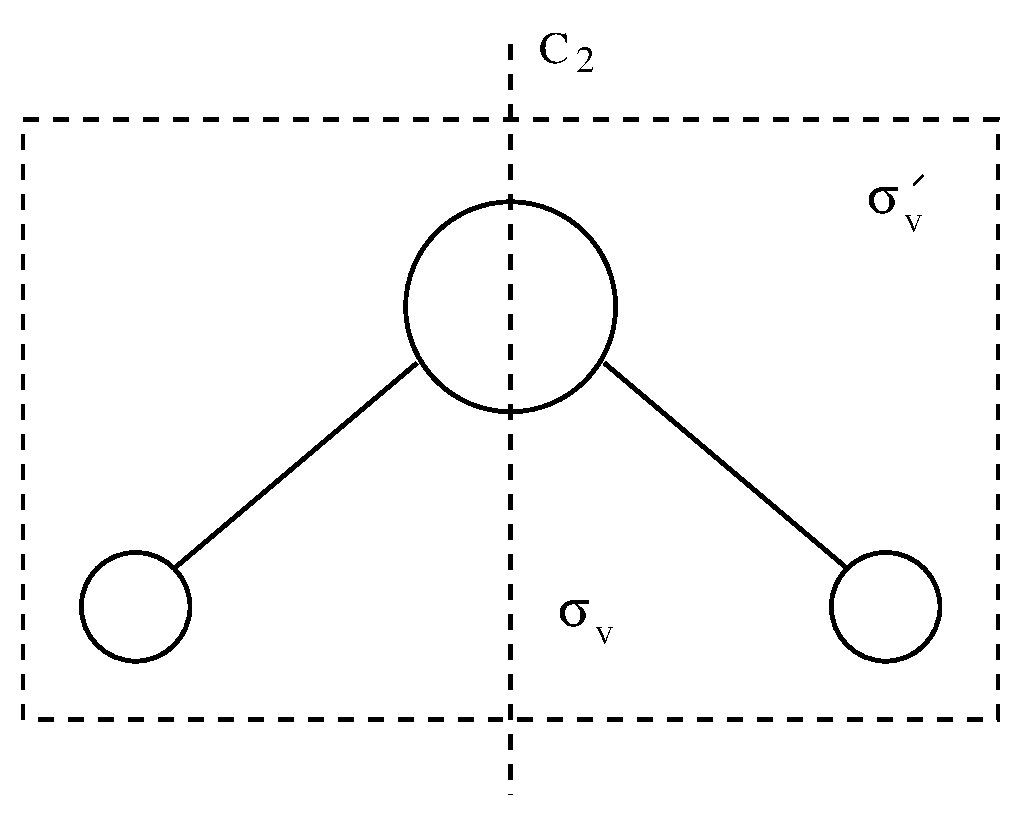
\epsfig{file={../fig/moleceau}}}   
 \caption{Water molecule. Symmetry group $C_{2v}$ corresponds to the set of
   operations: identity $E$, Rotation $C_2$ of angle $\pi$ around vertical
   axis, symmetry $\sigma_v$ with respect to plane perpendicular to paper sheet
   and symmetry $\sigma'_v$ with respect to sheet's plane.}
 \label{figmoleceau}
\end{figure}
Group $C_{2v}$ is one of the 32 possible point group
\cite{ma:group:Jones90,ph:solid:Ashcroft76}. Nomenclature is explained at
figure~\ref{figsymetr}. 
\begin{figure}[htb]
\centerline{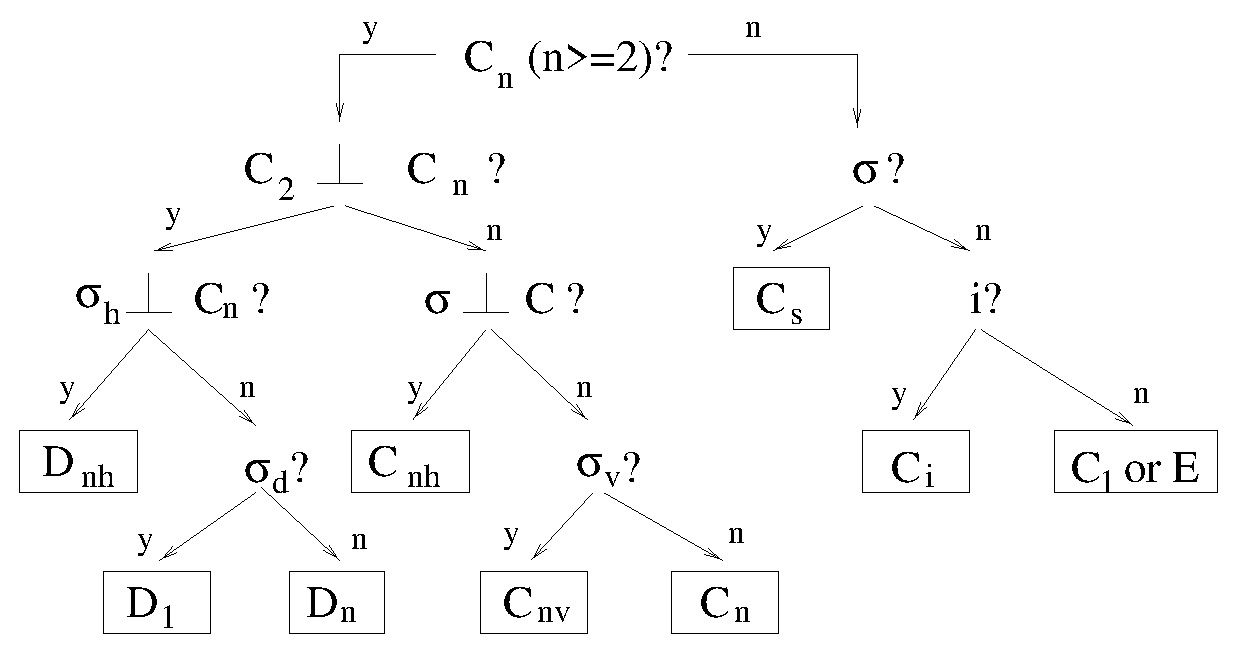
\epsfig{file={../fig/sym}}}   
 \caption{Nomenclature of symmetry groups in chemistry. The occurence of
   symmetry operations is successively tested, starting from the top of the
   tree. The tree is travelled through depending on the answers of questions,
   ``o'' for yes, and ``n'' for no. $C_n$ labels a rotations of angle
$2\pi/n$, $\sigma_h$ denotes symmetry operation with respect to a horizontal
plane (perpendicular the $C_n$ axis),
$\sigma_h$ denotes a symmetry operation with respect to the vertical plane
(going by the $C_n$ axis) and $i$ the inversion. Names of groups are framed.}
 \label{figsymetr}

\end{figure}
each of these groups can be characterized by tables of ``characters'' that
define possible irreducible representations
\index{irreducible representation}
for this group. Character table for group $C_{2v}$ is:
\begin{table}[hbt]\label{tabchar}
\caption{Character group for group $C_{2v}$.}
\begin{center}
\begin{tabular}{|l|r|r|r|r|}
$C_{2v}$ & $E$ & $C_2$ & $\sigma_v$ & $\sigma'_v$\\
\hline
$A_1$&1&1&1&1\\
$A_2$&1&1&-1&-1\\
$B_1$&1&-1&1&-1\\
$B_2$&1&-1&-1&1\\
\end{tabular}
\end{center}
\end{table}
All the representations of group $C_{2v}$ are one dimensional. There are four
representations labelled $A_1$, $A_2$, $B_1$ and $B_2$. In water molecule case,
space in nine dimension $e_i$
$i=1,\dots,9$. Indeed, each atom is represented by three coordinates. A
representation corresponds here to the choice of a linear combination $u$ of
vectors $e_{i}$ such that for each element of the symmetry group $g$, one has:
\begin{equation}
g(u)=M_gu.
\end{equation}
Character table provides the trace, for each operation $g$ of the
representation matrix $M_g$. As all representations considered here are one
dimensional, character is simply the (unique) eigenvalue of $M_g$.
Figure \ref{figmodesmol} sketches the nine representations of $C_{2v}$ group
for water molecule. It can be seen that space spanned by the vectors $e_i$ can
be shared into nine subspaces invariant by the operations $g$. Introducing
representation sum \cite{ma:group:Jones90}, considered representation $D$ can be written
as a sum of irreducible representations:
\begin{equation}
D=3A_1\oplus A_2\oplus2 B_1\oplus3 B_2.
\end{equation}
\begin{figure}
{\centering
\begin{tabular}[t]{ccc}

\epsffile{../fig/modesB2}
\epsffile{../fig/modesB2b}
\epsffile{../fig/modesB2bb}

\epsffile{../fig/modesB1}
\epsffile{../fig/modesB1b}
\epsffile{../fig/modesA2}

\epsffile{../fig/modesA1}
\epsffile{../fig/modesA1b}
\epsffile{../fig/modesA1bb}
\end{tabular} 
}
 \caption{Eigenmodes of $H_2O$ molecule. Vibrating modes are framed. Other
   modes correspond to rotations and translations.}
 \label{figmodesmol}
\end{figure}
It appears that among the nine modes, there are \index{mode} three translation
modes, and three rotation modes. Those mode leave the distance between the
atoms of the molecule unchanged. Three actual vibration modes are framed in
figure \ref{figmodesmol}.
Dynamics is in general defined by:
\begin{equation}
\frac{d^2x}{dt^2}=Mx
\end{equation}
where $x$ is the vector defining the state of the system in the $e_i$ basis.
Dynamics is then diagonalized in the coordinate system corresponding to the
three vibration modes. Here, symmetry consideration are sufficient to obtain
the eigenvectors. Eigenvalues can then be quickly evaluated once numerical
value of coefficients of $M$ are known.

\subsection{Two nuclei, one electron}
%%%%%%%%%%%%%%%%%
This case corresponds to the study of H$_2^+$ molecule
\cite{ph:mecaq:Pauling60,ph:mecaq:Cohen73}. 
The  Born-Oppenheimer approximation we use here consists in assuming that
protons are fixed (movement of protons is slow with respect to
movement of electrons). 
\begin{rem} This problem can be solved exactly. However, we present here the
  variational approximation that can be used for more complicated cases.
\end{rem}
The LCAO (Linear Combination of Atomic Orbitals) method we introduce here is a
particular case of the variational method. It consists in
approximating the electron wave function by a linear combination of
the one electron wave functions of the 
atom\footnote{That is: the space of solution is approximated by the
subspace spanned by the atom wave functions.}.  
\begin{equation}
\psi=a\psi_1+b\psi_2
\end{equation}
More precisely, let us choose as basis functions the functions
$\phi_{s,1}$ and $\phi_{s,2}$ that are $s$ orbitals centred on atoms $1$ and
$2$ respectively. This approximation becomes more valid as R is large (see
figure \ref{figH2plusS}).
\begin{figure}[htb]
 \centerline{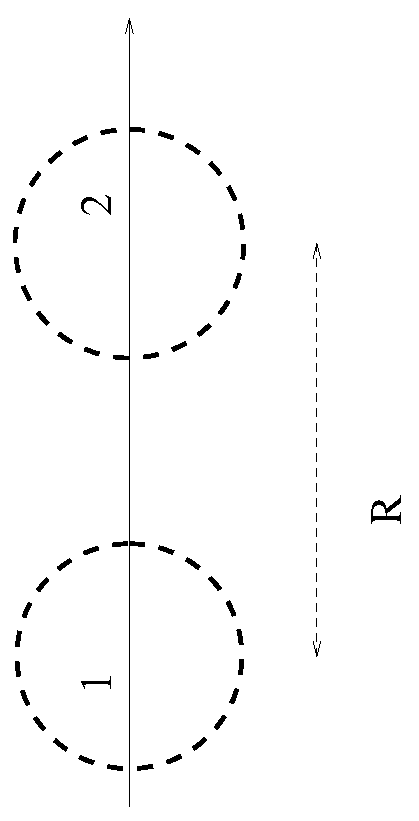
\epsfig{file={../fig/H2plusS}}}   
 \caption{{\bf Molecule H$^+_2$:} Choice of the functions $1s$
 associated to each of the hydrogen 
   atoms as basis used for the variational approach.}
 \label{figH2plusS}
\end{figure}
Problem's symmetries yield to write eigenvectors as:
\begin{eqnarray}
\psi_g&=&N_g(\psi_1+\psi_2)\\
\psi_u&=&N_u(\psi_1-\psi_2)
\end{eqnarray}
Notation using indices $g$ and $u$  is adopted, recalling the parity of the
functions: $g$ for {\it gerade}, that means even in German and
$u$ for {\it ungerade} that means odd in German. Figure
\ref{figH2plusLCAO} represents those two functions.
\begin{figure}[htb]
 
\epsffile{../fig/H2plusLCAO}
\epsffile{../fig/H2plusLCAO2}
 \caption{Functions $\psi_g$ and $\psi_u$ are solutions of variational
   approximation's problem on the basis of the two $s$ orbitals of the
   hydrogen atoms.}
 \label{figH2plusLCAO}
\end{figure}
Taking into account the hamiltonian allows to rise the degeneracy of the
energies as shown in diagram of figure \ref{figH2plusLCAOener}.
\begin{figure}[htb]
 \epsffile{../fig/H2plusLCAOener}
 \caption{Energy diagram for $H_2^+$ molecule deduced from LCAO method using
  orbitals $s$ of the hydrogen atoms as basis.}
 \label{figH2plusLCAOener}
\end{figure}

\subsection{N nuclei, n electrons}\label{secnnne}
%%%%%%%%%%%%%%%%%
In this case, consideration of symmetries allow to find eigensubspaces that
simplify the spectral problem. Those considerations are related to point
groups representation theory. When atoms of a same molecule are located in a
plane, this plane is a symmetry element. In the case of a linear molecule, any
plane going along this line is also symmetry plane. Two types of orbitals are distinguished:
\begin{defn}
Orbitals $\sigma$ are conserved by reflexion with respect to the symmetry
plane. 
\end{defn}
\begin{defn}
Orbitals $\pi$ change their sign in the reflexion with respect to this plane. 
\end{defn}
Let us consider a linear molecule. For other example, please refer to
\cite{ph:mecaq:Pauling60}. 
\begin{exmp}
{\bf Molecule BeH$_2$}.
We look for a wave function in the space spanned by orbitals $2s$ and $z$ of
the beryllium atom Be and by the two orbitals $1s$ of the two hydrogen
atoms. Space is thus four dimension (orbitals $x$ and $y$ are not used) and
the hamiltonian to diagonalize in this basis is written in general as a matrix
$4\times 4$. 
Taking into account symmetries of the molecule considered allows to put this
matrix as  {\it block diagonal matrix}. Let us choose the following basis as
approximation of the state space:
\{$2s,z,1s_1+1s_2,1s_1-1s_2$\}. Then symmetry considerations imply that
orbitals have to be:
\begin{eqnarray}
\sigma_s&=&\alpha_12s+\beta_1(1s_1+1s_2)\\
\sigma_s^*&=&\alpha_22s-\beta_2(1s_1+1s_2)\\
\sigma_p&=&\alpha_3z+\beta_3(1s_1-1s_2)\\
\sigma_p^*&=&\alpha_4z-\beta_4(1s_1-1s_2)
\end{eqnarray}
Those bindings are delocalized over three atoms and are sketched at figure
\ref{figBeH2orb}. 
\begin{figure}[htb]
 \centerline{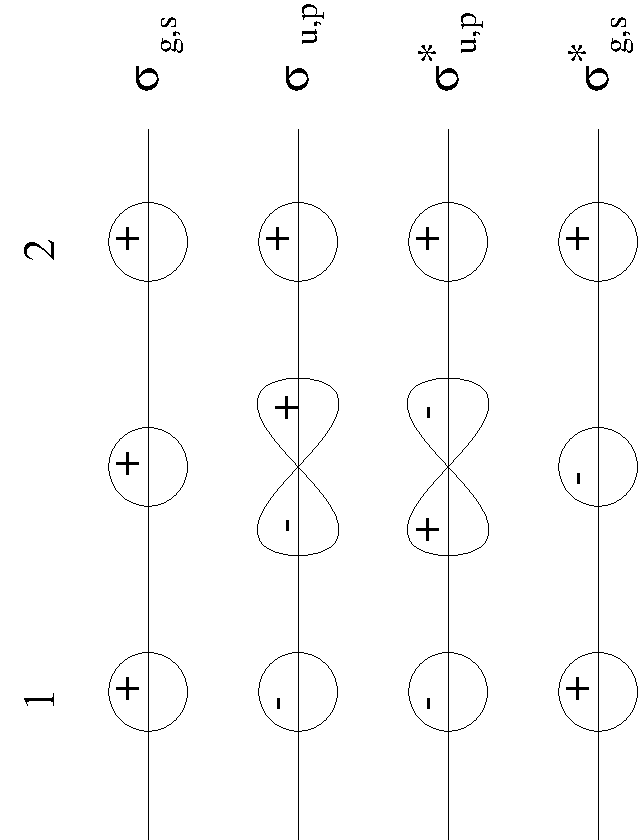
\epsfig{file={../fig/BeH2orb}}}   
 \caption{Study of $H_2^+$ molecule by the LCAO method. The basis
   chosen is the two orbitals $s$ of hydrogen atoms.}
 \label{figBeH2orb}
\end{figure}
We have two binding orbitals and two anti--binding orbitals. Energy diagram
is represented in figure \ref{figBeH2ene}.In the fundamental state, the four
electrons occupy the two binding orbitals.
\begin{figure}[htb]
 \centerline{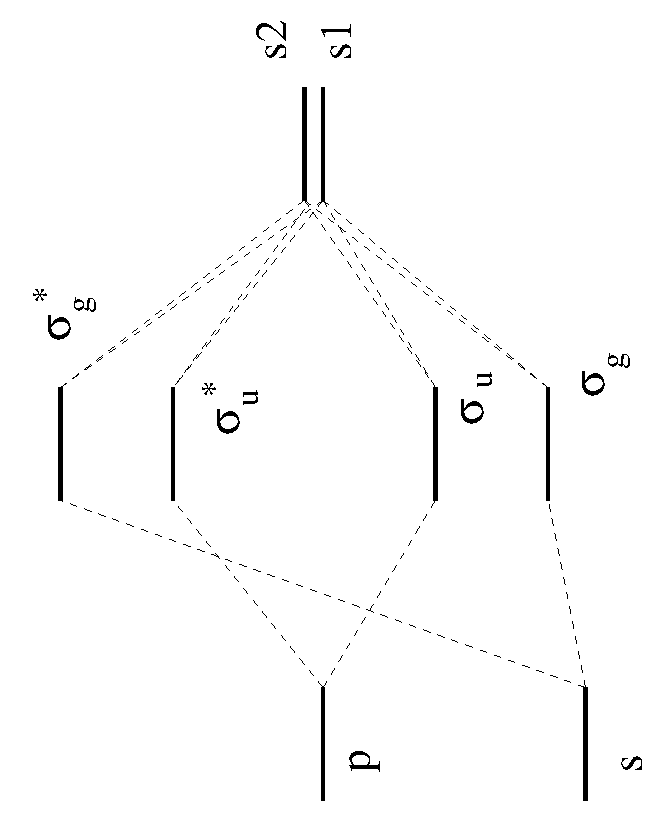
\epsfig{file={../fig/BeH2ene}}}   
 \caption{Energy diagram for $H_2^+$ molecule by the LCAO method. The basis
   chosen is the two orbitals $s$ of hydrogen atoms.}
 \label{figBeH2ene}
\end{figure}
\end{exmp}
Experimental study of molecules show that characteritics of bondings depend
only slightly on on nature of other atoms. The
problem is thus simplified in considering $\sigma$ molecular orbital as being
dicentric, that means located between two atoms. Those orbitals are called
hybrids. 
\begin{exmp}
let us take again the example of the  BeH$_2$ molecule. This molecule is
linear. This geometry is well described by the $s-p$ hybridation. Following
hybrid orbitals are defined: 
\begin{eqnarray}
d_1&=&\frac{1}{\sqrt{2}}(s+z)\\
d_2&=&\frac{1}{\sqrt{2}}(s-z)
\end{eqnarray}
Instead of considering the basis \{$2s,z,1s_1,1s_2$\}, basis
\{$d_1,d_2,1s_1,1s_2$\} is directly considered. Spectral problem is thus from
the beginning well advanced.
\end{exmp}
\section{Crystals}\label{secsolidmq}
%%%%%%%%%%%%%%%%%%%%%%%%%%%%%%
\subsection{Bloch's theorem}\label{sectheobloch}
%%%%%%%%%%%%%%%
Consider following spectral problem:
\begin{prob}
Find $\psi(r)$ and $\epsilon$ such that
\begin{equation}
[-\frac{\hbar^2}{2m}\nabla^2+V(r)]\psi(r)=\epsilon\psi(r)
\end{equation}
where $V(r)$ is a periodical function.
\end{prob}
Bloch's theorem\cite{ma:equad:Dautray5,ph:solid:Kittel67,ph:physt:Diu89}
allows\index{Bloch theorem} to look for eigenfunctions under a form
that takes into account symmetries of considered problem.
\begin{thm}\label{theobloch}{\bf Bloch's theorem.} If $V(r)$ is periodic then
  wave function $\psi$ solution of the spectral problem can bne written:
\begin{equation}
\psi(r)=\psi_k(r)=e^{ikr}u_k(r)
\end{equation}
with $ u_k(r)=U_k(r+R)$ (function $u_k$ has the lattice's periodicity).  
\end{thm}
\begin{pf}
Operator $-\frac{\hbar^2}{2m}\nabla^2+V(r)$ commutes with translations
$\tau_j$ defined by $\tau_a\psi(r)=\psi(r+a)$.
Eigenfunctions of $\tau_a$ are such that:
\begin{equation}
\tau_a\psi=\psi
\label{tra}
\end{equation}
Properties of Fourier transform\index{Fourier transform} allow to evaluate the
eigenvalues of $\tau_j$. Indeed, equation \ref{tra} can be written:
\begin{equation}
\delta(x-a)*\psi(r)=\psi(r)
\end{equation}
where $*$ is the space convolution. Applying a Fourier transform to previous
equation yields to:
\begin{equation}
e^{-2i\pi ka}\hat{\psi}=\hat{\psi}
\end{equation}
That is the eigenvalue is $\lambda=e^{-2i\pi k_na}$ with $k_n=n/a$
\footnote{%%%%%%%%%%%%%
So, each irreducible representation\index{irreducible representation} of
the translation group is characterized by a vector $k$. This representation is
labelled $\Gamma_k$.}.%%%%%%%%%%%%%%%
On another hand, eigenfunction can always be written:
\begin{equation}
\psi_k(r)=e^{ikr}u_k(r).
\end{equation}
Since $u_k$ is periodical\footnote{%%%%%
Indeed, let us write in two ways the action of $\tau_a$ on $\phi_k$:
\begin{equation}
\tau_a\psi_k=e^{ika}\psi_k
\end{equation}
and
\begin{equation}
\tau_a\psi_k=e^{ik(r+a)}u_k(r+a)
\end{equation}
}%%%%%%%%%%%%%%%%%%%%%
theorem is proved.
\end{pf}
\subsection{Free electron model}
%%%%%%%%%%%%%%%%%%%%%%%%%%%%%
Hamiltonian can be written\cite{ph:solid:Kittel67,ph:solid:Callaway64}
here: 
\begin{equation}
H=-\frac{\hbar^2}{2m}\nabla^2+V(r)
\end{equation}
where $V(r)$ is the potential of a periodical box of period $a$
(see figure \ref{figpotperioboit})
\ref{figeneeleclib}. 
\begin{figure}[htb]
 \centerline{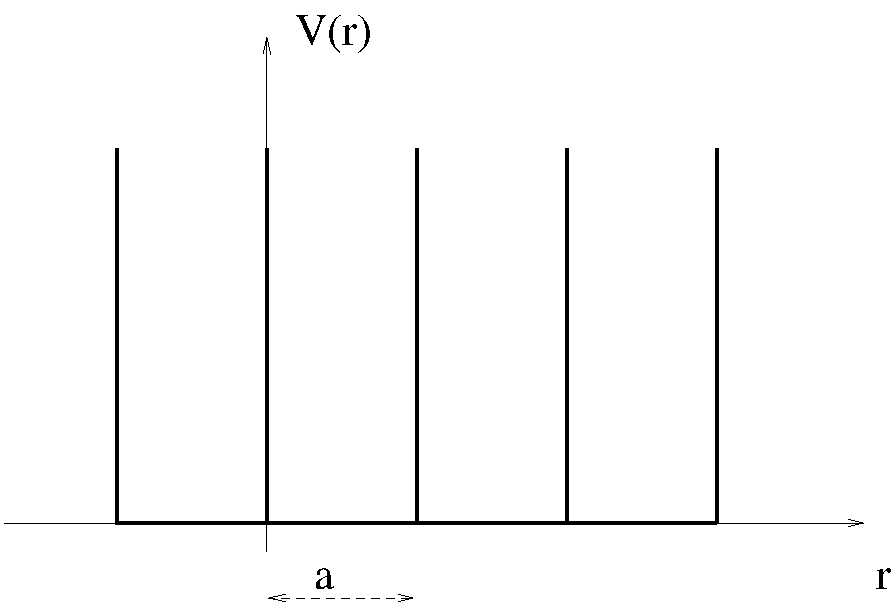
\epsfig{file={../fig/potperioboit}}}   
 \caption{Potential in the free electron approximation.}
 \label{figpotperioboit}
\end{figure}
Eigenfunctions of $H$ are eigenfunctions of $\nabla^2$
(translation invariance) that verify boundary conditions. Bloch's theorem
implies that $\phi$ can be written:
\begin{equation}
\psi_k=e^{ikr}u_k(\bar{r})
\end{equation}
where  $u_k(\bar{r})$ is a function that has crystal's
symmetry\index{crystal}, that means it is translation invariant:
\begin{equation}
u_k(\bar{r}+\bar{R}_i)=u_k(\bar{r})
\end{equation}
Here (see \cite{ph:solid:Callaway64}), any function $u_k$ that can be written
\begin{equation}
u_k(\bar{r})=e^{iK_nr}
\end{equation}
is valid. Injecting this last equation into  Schr\"odinger equation yields to
following energy expression: 
\begin{equation}
E_k=\frac{\hbar^2}{2m}|k+K_n|^2
\end{equation}
where $K_n$ can take values $\frac{2n\pi}{a}$, where $a$ is lattice's period
and  $n$ is an integer.
Plot of $E$ as a function of $k$ is represented in figure
\ref{figeneeleclib}. 
\begin{figure}[htb]
 \centerline{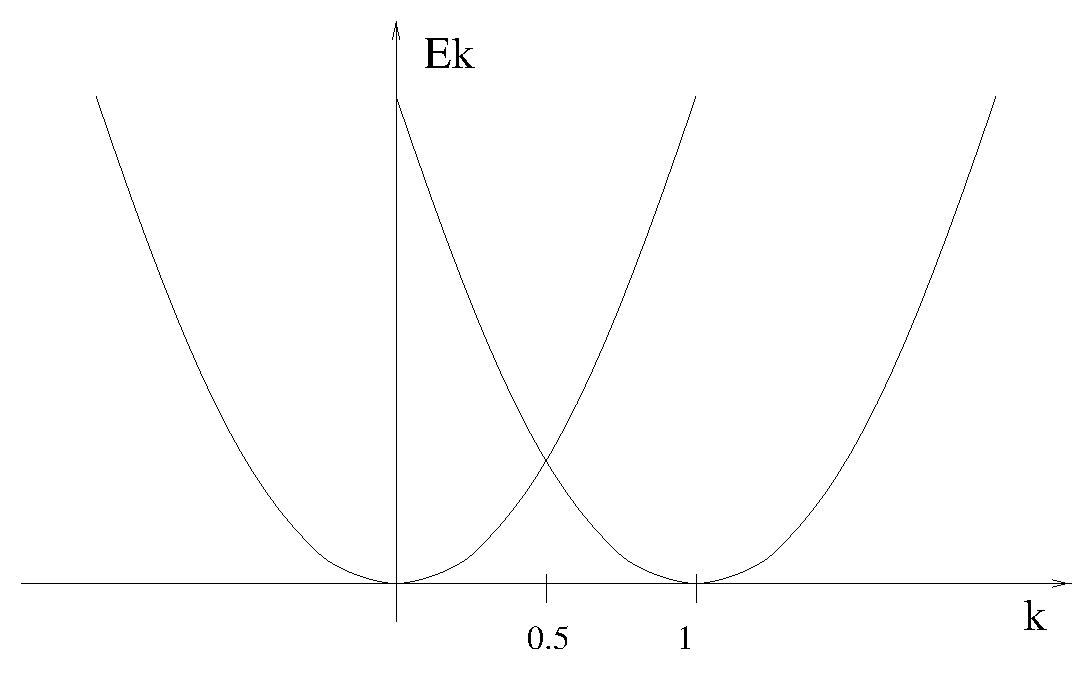
\epsfig{file={../fig/eneeleclib}}}   
 \caption{Energy of mode $k$ in the free electron approximation (electron in a
   box).}
 \label{figeneeleclib}
\end{figure}

\subsection{Quasi-free electron model}
%%%%%%%%%%%%%%%%%%%%%%%%%%%%%
Let us show that if the potential is no more the potential of a periodic box,
degeneracy at $k=\frac{K_1}{2}$ is erased. Consider for instance a potential
$V(x)$ defined by the sum of the box periodic potential plus a periodic
perturbation: 
\begin{equation}
V(x)=V_{box}+\epsilon e^{iK_1r}
\end{equation}
In the free electron model functions
\begin{eqnarray}
\psi_{1k}&=&e^{ikr}\\
\psi_{2k}&=&e^{ikr}e^{iK_1r}
\end{eqnarray}
are degenerated. Diagonalization of Hamiltonian in this basis (perturbation
method for solving spectral problems, see section \ref{chapresospec}) shows
that degeneracy is erased by the perturbation. 
\subsection{Thigh binding model}
%%%%%%%%%%%%%%%%%%%%%%%%%%%
Tight binding approximation\cite{ph:solid:Ashcroft76}  consists in
approximating the state space by the space spanned by atomic orbitals centred
at each node of the lattice. That is, each eigenfunction is assumed to
be of the
form: 
\begin{equation}
\psi(r)=\sum_j c_j\phi_{at}(r-R_j)
\end{equation}
Application of Bloch's theorem yields to look for $\psi_k$ such that
it can be written:
\begin{equation}
\psi_k(r)=e^{ikr}u_k(r)
\end{equation}
Identifying $u_k(r)$ and $u_k(r+R_i)$, it can be shown that
$c_l=e^{ikK_l}$. Once more, symmetry considerations fully determine the
eigenvectors. Energies are evaluated from the expression of the
Hamiltonian. Please refer to 
\cite{ph:solid:Ashcroft76} for more details. 


\section{Exercises}
%%%%%%%%%%%%%%%%%%%

\begin{exo}
Give the name of the symmetry group molecule $NH_{3}$ belongs to.
\end{exo}
\begin{exo}
Parametrize the vibrations of molecule  $NH_{3}$ and expand it in a sum of
irreducible representations.
\end{exo}

\begin{exo}
Propose a basis for the study of molecule $BeH_{2}$ different from those
presented at section \ref{secnnne}.
\end{exo}
\begin{exo}
Find the eigenstates as well as their energies of a system constituted
by an electron in a square box
of side $a$ (potential zero for $-a/2<x<a/2$ and
$-a/2<y<+a/2$, potential infinite elsewhere). 
What happens if to this potential is added a perturbation of value $\epsilon$
on a quarter of the box
($0<y<a/2$ and $0<y<a/2$)?
Calculate by perturbation the new energies and eigenvectors. Would symmetry
considerations have permitted to know in advance the eigenvectors?
\end{exo}



\chapter{Statistical physics}\label{chapphysstat}
%%%%%%%%%%%%%%%%%%%%%%%%%%%%
\section{Introduction}
%%%%%%%%%%%%%%%%%%%%%
Statistical physics goal is to describe matter's properties at macroscopic
scale from a microscopic description (atoms, molecules, etc\dots). The great
number of particles constituting a macroscopic system justifies a
probabilistic description of the system. Quantum mechanics (see
chapter~\ref{chapmq})  allows to describe part of systems made by a large
number of particles: Schr\"odinger equation provides the various accessible
states as well as their associated energy. Statistical physics allows to
evaluate occupation probabilities $P_l$ of a quantum state $l$. It introduces
fundamental concepts as temperature, heat\dots

Obtaining of probability $P_l$ is done using the statistical physics principle
that states that physical systems tend to go to  a state of ``maximum
disorder'' \cite{ph:physt:Reif64,ph:physt:Diu89}. A disorder measure is given
by the statistical entropy\footnote{%%%%%
This formula is analog to the information entropy chosen by Shannon in his
information theory\cite{ph:physt:Shannon49}.}\index{entropy}
\begin{equation}
S=-k_B\sum P_l \ln P_l
\end{equation}
The statistical physics principle can be enounced as:
\begin{postulat}
At macroscopic equilibrium, statistical distribution of microscopic states is,
among all distributions that verify external constraints imposed to the
system, the distribution that makes statistical entropy maximum.
\end{postulat}
\begin{rem}
This problem corresponds to the classical minimization (or maximization)
problem presented at 
section \ref{chapmetvar}) which can be treated by Lagrange multiplier method.
\index{Lagrange multiplier} 
\end{rem}
\section{Entropy maximalization}\label{secmaxient}
%%%%%%%%%%%%%%%%%%%%%%%%%%%%%%%%%%%%%%%%%%%
The mathematical problem associated to the calculation of occupation
probability $P_l$ is here presented:\index{maximalization}
In general, a system is described by two types of variables. External
variables $y^i$ whose values are fixed at $y_j$ by the exterior and internal
variables $X^i$ taht are free to fluctuate, only their mean being fixed to
$\bar{X^i}$. Problem to solve is thus the following:
\begin{prob}
Find distribution probability $P_l$ over the states $(l)$ of the
considered system 
that maximizes the entropy
\begin{equation}
S=-k_B\sum P_l \ln (P_l)
\end{equation}
and that verifies following constraints:
\begin{eqnarray}
\sum X_{l}^iP_l&=&\bar{X^i}\\
\sum P_l&=&1
\end{eqnarray}
\end{prob}
Entropy functional maximization is done using Lagrange multipliers
technique. Result is:
\begin{equation}
P_l=\frac{1}{Z}e^{-\lambda_1 X^{1}_l-\lambda_2 X^{2}_l- ...}
\end{equation}
where function $Z$, called partition function,
\index{partition function}
is
defined by:
\begin{equation}
Z=\sum_{(l)} e^{-\lambda_1 X^{1}_l-\lambda_2 X^{2}_l- ...}
\end{equation}
Numbers $\lambda_i$ are the Lagrange multipliers of the maximization problem
considered.
\begin{exmp}
In the case where energy is free to fluctuate around a fixed average, Lagrange
multiplier is:
\begin{equation}
\beta=\frac{1}{k_BT}
\end{equation}
where $T$ is temperature.\index{temperature} We thus have a mathematical
definition of temperature.
\end{exmp}
\begin{exmp}
In the case where the number of particles is free to fluctuate around a fixed
average, associated Lagrange multiplier is noted $\beta\mu$ where $\mu$ is
called the chemical potential.
\end{exmp}
Relations on means\footnote{They are used to determine Lagrange multipliers
$\lambda_i$ from associated means $\bar{X_i}$} can be written as:
\begin{equation}
-\frac{\partial}{\partial \lambda_i}\ln Z(y,\lambda_1,\lambda_2,...) =
\bar{X_i} 
\end{equation}
It is useful to define a function $L$ by:
\begin{equation}
L=\ln Z(y,\lambda_1,\lambda_2,...)
\end{equation}
It can be shown\footnote{%%%%%%%
By definition
\begin{equation}
S=-k_B\sum P_l \ln (P_l)
\end{equation}
thus
\begin{equation}
S/k=-\sum P_l\ln(\frac{1}{Z}e^{-\lambda_1 X^{1}_l-\lambda_2 X^{2}_l- ...})
\end{equation}
\begin{equation}
S/k=1\ln Z+\lambda_1 \bar{X^{1}_l}+\lambda_2 \bar{X^{2}_l}+ ...
\end{equation}
} that:
\begin{equation}
S/k=\sum \lambda_i \bar{X^i}+\ln(Z)
\end{equation}
This relation that binds $L$ to $S$ is called a {\bf Legendre
  transform}.\index{Legendre transformation} 
$L$ is function of the $y^i$'s and  $\lambda_j$'s, $S$ is a function of
the $ y^i$'s and $\bar{X^j}$'s.
\section{Canonical distribution in classical mechanics}\label{secdistclassi} 
%%%%%%%%%%%%%%%%%%%%%%%%%%%%%%%%%%%%%%%%%%%%%%%%%%%%%%%%%%
Consider a system for which only the energy is fixed. Probability for this
system to be in a quantum state $(l)$ of energy $E_l$ is given (see previous
section) by:
\begin{equation}
P_l=\frac{1}{Z}e^{-E_l/k_BT}
\end{equation}
Consider a classical description of this same system. For instance, consider a
system constituted by $N$ particles whose position and momentum are noted $q_i$
and $p_i$, described by the classical hamiltonian $H(q_i,p_i)$.
A classical probability density $w^c$ is defined by:
\begin{equation}\label{eqdensiprobaclas}
w^c(q_i,p_i)=\frac{1}{A}e^{-H(q_i,p_i)/k_BT}
\end{equation}
Quantity $w^c(q_i,p_i)dq_idr_i$ represents the probability for the system to
be in the phase space volume between hyperplanes  $q_i,p_i$ and $q_i+dq_i,
p_i+dp_i$. 
Normalization coefficients $Z$ and $A$ are proportional.
\begin{equation}
A=\int dq_1...dq_n\int dp_1...dp_n e^{-H(q_i,p_i)/k_BT}
\end{equation}
One can show \cite{ph:physt:Diu89} that
\begin{equation}
Z=\frac{1}{(2\pi\hbar)^{3N}}A
\end{equation}
$2\pi\hbar^N$ being a sort of quantum state volume.
\begin{rem}
This quantum state volume corresponds to the minimal precision allowed in the
phase space from the Heisenberg uncertainty principle:
\index{Heisenberg uncertainty principle} 
\begin{equation}
\Delta x \Delta p > \hbar
\end{equation}
\end{rem}
Partition function provided by a classical approach becomes thus:
\begin{equation}
Z=\frac{1}{(2\pi\hbar)^N}\int dq_1...dq_n\int dp_1...dp_n e^{-H(q_i,p_i)/k_BT}
\end{equation}
But this passage technique from quantum description to classical description
creates some compatibility problems. For instance, in quantum mechanics, there
exist a postulate allowing to treat the case of a set of identical particles.
Direct application of formula of equation \ref{eqdensiprobaclas} leads to
wrong results (Gibbs paradox). In a classical treatment of set of identical
particles, a postulate has to be artificially added to the other statistical
mechanics postulates:
\begin{postulat}
Two states that does not differ by permutations are not considered as
different. 
\end{postulat}
This leads to the classical partition function for a system of $N$ identical
particles: 
\begin{equation}
Z=\frac{1}{N!}\frac{1}{(2\pi\hbar)^{3N}}\int\prod dp^{3}_i dq^{3}_i
e^{-H(q_i,p_i)/k_BT} 
\end{equation}

\section{Constraint relaxing}\label{secrelacont}
%%%%%%%
We have defined at section \ref{secmaxient} external variables, fixed by the
exterior, and internal variables free to fluctuate around a fixed mean.
Consider a system  $L$ being described by $N+N'$ internal variables
\index{constraint} $n_1,\dots,n_N,X_1,\dots,X_{N'}$. 
This system has a partition function $Z^{L}$. Consider now a system $F$, such
that variables $n_i$are this time considered as external variables having
value $N_i$. This system $F$ has (another) partition function we call
$Z^{F}$. System $L$ is obtained from system $F$ by constraint
relaxing. Here is theorem that binds internal variables $n_i$ 
of system  $L$ to partition function $Z^F$ of system $F$ :
\begin{thm}
Values $n_i$ the most probable in system $L$ where
$n_i$ are free to fluctuate are the values that make zero the differential of
partition function $Z^{F}$  where the $n_i$'s are fixed. 
\end{thm}
\begin{pf}
Consider the description where the $n_i$'s are free to fluctuate. Probability
for event $n_1=N_1$,$\cdots$,$n_N=N_N$ occurs is:
\begin{equation}
P(n_1=N_1,\cdots,n_N=N_N)=\sum_{(l)/n_1=N_1,\cdots,n_N=N_N}P^{L}_l
\end{equation}
So
\begin{eqnarray}
\lefteqn{P(n_1=N_1,\cdots,n_N=N_N) = }\\
&&\frac{1}{Z^{nl}} e^
{-\lambda_{n_1}N_1-\cdots-\lambda_{n_N}N_N} \sum_{(l)/n_1 =
N_1,\cdots,n_N=N_N} e^ {-\lambda_{X_1}\bar X_1-\lambda_{X_2}\bar X_2} 
\end{eqnarray}
Values the most probable make zero differential
$dP(n_1=N_1,\cdots,n_N=N_N)$ (this corresponds to the maximum of a
(differentiable) function $P$.).
So
\begin{equation}
d\log(Z^{F})=\sum_i \frac{\partial \log(Z^{F})}{\partial n_i}dn_i=0
\end{equation}
\end{pf}
%%%%%%%%%%%
\begin{rem}
This relation is used in chemistry: it is the fundamental relation of chemical
reaction. In this case, the $N$ variables
$n_i$ represent the numbers of particles of the $N$ species  $i$ and $N'=2$
with $X_1=E$ (the energy of the system)  and $X_2=V$ (the volume of the
system). Chemical reaction equation gives a binding on variables
$n_i$ that involves stoechiometric coefficients.
\end{rem}
Let us write a Gibbs-Duheim type relation
\index{Gibbs-Duheim relation}:
\begin{equation}
S^{F}/k=\lambda_{X_1}\bar X_1+\lambda_{X_2}\bar X_2+\ln (Z^{F})
\end{equation}
\begin{equation}
S^{L}/k=\lambda_{X_1}\bar X_1+\lambda_{X_2}\bar X_2+\lambda_{n_1}\bar{n_1}+\cdots+\ln (Z^{L})
\end{equation}
At thermodynamical equilibrium $S^{F}=S^{L}$, so:
\begin{equation}
\lambda_{n_i}=\frac{\partial \ln (Z^{F})}{\partial n_i}
\end{equation}
\begin{exmp}
This last equality provides a way to calculate the chemical potential of the
system.\index{chemical potential} 
\begin{equation}
\mu_i=\frac{\partial \ln (Z^{F})}{\partial n_i}
\end{equation}
In general one notes $-\ln(Z^{F})=G$.
\end{exmp}
\begin{exmp}
Consider the case where variables $n_i$ are the numbers of particles of species
$i$. If the particles are independent, energy associated to a state describing
the $N$ particles (the set of particles of type $i$ being in state $l_i$) is
the sum of the $N$ energies associated to states $l_i$. Thus:
\begin{equation}
\ln Z^F(\lambda_{X_1},\lambda_{X_2},n_1,n_2)=\ln
Z^F_1(\lambda_{X_1},\lambda_{X_2},n_1)+\dots+\ln
Z^F_N(\lambda_{X_1},\lambda_{X_2},n_N) 
\end{equation}
where $Z^F_i(\lambda_{X_1},\lambda_{X_2},n_i)$ represents the partition
function of the system constituted only by particles of type $i$, for which
the value of variable $n_i$ is fixed. So:
\begin{equation}
\frac{\partial \ln Z^F_1}{\partial n_1} dn_1+\dots+\frac{\partial \ln
Z^F_N}{\partial n_N} dn_N=0 
\end{equation}
\end{exmp}
\begin{rem}
Setting $\lambda_1=\beta$,$\lambda_2=\beta p$ and $\lambda_{n_1}=-\beta\mu$
with $G=-k_BT\ln Z^{nf}$, we have $G(T,p,n)=E+pV-TS$ and
$G'(T,p,\mu)=E+pV-TS-\mu-{n_1}$. This is a Gibbs-Duheim relation.
\end{rem}
\begin{exmp}
We propose here to prove the
Nernst formula\index{Nernst formula} describing an oxydo-reduction
reaction.\index{oxydo-reduction} This type of chemical reaction can be
tackled using previous formalism. Let us precise notations in a particular
case. Nernst formula demonstration that we present here is different form
those classically presented in chemistry books. Electrons undergo a potential
energy variation going from solution potential to metal potential.
This energy variation can be seen as the work got by the system or as the
internal energy variation of the system, depending on the considered system is
the set of the electrons or the set of the electrons as well as the solution
and the metal. The chosen system is here the second. Consider the free
enthalpy function $ G(T,p,n_i,E_p)$. Variables $n_i$ and $E_p$ are free to
fluctuate. They have values such that $G$ is minimum. let us calculate the
differential of $G$:
\begin{equation}
dG(T,p,n_i,E_p)=\frac{\partial G}{\partial T} dT +\frac{\partial
G}{\partial p} dp+\sum_i\frac{\partial G}{\partial n_i}\
dn_i+\frac{\partial G}{\partial E_p} dE_p
\end{equation}
Using definition\footnote{%%%%%%%
the internal energy $U$ is the sum of the kinetic energy and the potential
energy, so as $G$ can be written itself as a sum:
\begin{equation}
G=U+pV-TS
\end{equation}}
%%%%%%%%%%
of $G$:
\begin{equation}
\frac{\partial G}{\partial E_p}=1
\end{equation}
one gets:
\begin{equation}
0=\sum_i\mu_idn_i+dE_p
\end{equation}
If we consider reaction equation:
\begin{equation}
Ox+n\bar e\longrightarrow Red
\end{equation}
\begin{equation}
0=\sum_i \mu_i \nu_i d\xi +nq(V_{red}-V_{ox})
\end{equation}
So:
\begin{equation}
V_{red}-V_{ox}=\frac{\sum_i\nu_i\mu_i}{nF}
\end{equation}
$dG$ can only decrease. Spontaneous movement of electrons 
is done in the sense that implies $dE_p < 0$. As $dE_p^{ext}=-dE_p^{int}$ we
chose as definition of electrical potential: 
\begin{equation}
V^{ext}=-V^{int}
\end{equation}
Nernst formula deals with the electrical potential seen by the exterior.
\end{exmp}


\section{Some numerical computation in statistical physics}
%%%%%%%%%%%%%%%%%%%%%
In statistical physics, mean quantities evaluation can be done using by
Monte--Carlo methods. in this section, a simple example is presented.
\begin{exmp}
Let us consider a Ising model. In this spin system, energy can be written:
\begin{equation}
E=-J\sum_i\sum_k S_iS_k-B\sum S_k
\end{equation}
The following Metropolis algorithm\cite{ma:compu:Stauffer93,ma:compu:Koonin90}
is used \index{Metropolis} 
to simulate probabilities $exp(-E/k_BT)$:
\begin{enumerate}
\item select spin $S_k$ to consider.
\item evaluate variation of energy $\Delta E=E_{new}-E_{old}$ associated
  to a possible split of spin $S_k$.
\item compare a random number $z$ between zero and one with probability $p=exp(-\Delta E/k_BT)$.
\item split spin number $k$ (that is do $S_k=-S_k$) i=f and only if $z<p$.
\item use the obtained configuration to compute mean quantities.
\end{enumerate}
\end{exmp}



\section{Exercise}
%%%%%%%%%%%%%%%%%%%%%

\begin{exo}
Consider a chain of $N$ nonlinear coupled oscillators. Assuming known the
(deterministic) equation governing the dynamics of the particles, is that
possible to define a system's temperature? Can one be sure that a system of
coupled nonlinear oscillators will evolve to a state well described by
statistical physics? Do a bibliographic research on this subject, in
particular on Fermi--Ulam--Pasta model.
\end{exo}



\chapter{N body problems and statistical equilibrium}\label{chapNcorpsstat} 
%%%%%%%%%%%%%%%%%%%%%%%%%%
\section{N body problems}
%%%%%%%%%%%%%%%%%%%%%%%%
At chapter \ref{chapproncorps}, $N$ body problem was treated in the quantum
mechanics framework. In this chapter, the same problem is tackled using
statistical physics. The number $N$ of body in interaction is assumed
here to be large, of the order of Avogadro number.
Such types of N body problems can be classified as follows:
 \begin{itemize}
\item Particles are undiscernable. System is then typically a gas. In a
  classical approach, partition function has to be described using a
  corrective factor
$\frac{1}{N!}$ (see section \ref{secdistclassi}). Partition function can be
factorized in two cases: particles are independent (one speaks about perfect
gases)\index{perfect gas}
Interactions are taken into account, but in the frame of a {\bf mean field
  approximation}\index{mean field}. This allows to considerer particles as if
they were independent (see van der Waals model at section
\ref{secvanderwaals})
In a quantum mechanics approach, Pauli principle can be included in the most
natural way. The suitable description is the grand-canonical description: 
number of particles is supposed to fluctuate around a mean value.
The Lagrange multiplier associated to the particles number variable is the
chemical potential $\mu$. Several physical systems can be described by quantum
perfect gases (that is a gas where interactions between particles are
neglected): a fermions gas can modelize a semi--conductor. A boson gas can
modelize helium and described its properties at low temperature. 
If bosons are photons (their chemical potential is zero), the black body
radiation can be described.
\item Particles are discernable. This is typically the case of particles on a
  lattice. Such systems are used to describe for instance magnetic properties
  of solids. Taking into account the interactions between particles, phase
  transitions like paramagnetic--ferromagnetic transition can be
  described\footnote{%%%%%%%%%%%%%%%
A mean field approximation allows to factorize the partition
function. Paramagnetic--ferromagnetic transition is a second order transition:
the two phases can coexist, on the contrary to liquid vapour transition that
is called first order transition.}. Adsorption phenomenom can be modelized by
a set of independent particles in equilibrium with a particles reservoir
(grand-canonical description).
\end{itemize}
Those models are described in detail in \cite{ph:physt:Diu89}.
In this chapter, we recall the most important properties of some of them.

\section{Thermodynamical perfect gas}\label{secgasparfthe}
%%%%%%%%%%%%%%%%%%%%
In this section, a perfect gas model is presented: all the particles are
independent, without any interaction.
\begin{rem}
A perfect gas corresponds to the case where the kinetic energy of the particles
is large with respect to the typical interaction energy. Nevertheless,
collisions between particles that can be neglected are necessary for the
thermodynamical equilibrium to establish.
\end{rem}
Classical approximation (see section \ref{secdistclassi}) allows to replace
the sum over the quantum states by an integral of the exponential of the
classical hamiltonian $H(q_i,p_i)$. The price to pay is just to take into
account a proportionality factor $\frac{1}{2\pi \hbar}$. Partition function
$z$ associated to one particle is:
\begin{equation}
z=\frac{1}{2\pi \hbar}\int dq_i dp_i e^{-\beta H(p,q)}
\end{equation}
\begin{equation}
z=\frac{1}{2\pi \hbar}\int dq^3 \int dp^3 e^{-\beta H(p,q)}
\end{equation}
Partition function $z$ is thus proportional to $V$ :
\begin{equation}
z=A(\beta) V
\end{equation}
Because particles are independent, partition function $Z$ for the whole system
can be written as:
\begin{equation}
Z=\frac{1}{N!}z^N
\end{equation}
It is known that pressure (proportional to the Lagrange multiplier associated
to the internal variable ``volume'') is related to the natural logarithm of
$Z$; more precisely if one sets:
\begin{equation}
F=-k_BT\log Z
\end{equation}
then
\begin{equation}
p=-\frac{\partial F}{\partial V}.
\end{equation}
This last equation and the expression of $Z$ leads to the famous perfect gas
state equation:
\begin{equation}
pV=Nk_BT
\end{equation}

\section{Van der Waals gas}\label{secvanderwaals}
%%%%%%%%%%%%%%%%%%%%%%%%%%
Van der Waals\footnote{Johannes Diderik van der Waals received the
physics Nobel price in 1910.} gas model\index{Van der Walls gas} is a
model that also 
relies on classical approximation, that is on the repartition function that
can be written:
\begin{equation}
Z=\frac{1}{N!} \frac{1}{h^{3N}}\int\int d^3p_1\dots d^3p_N
d^3r_1\dots d^3r_N  e^{-\frac{H}{k_BT}}
\end{equation}
where the function $H(p_1 ,\dots ,p_N,r_1 ,\dots ,r_N)$ is the hamiltonian of
the system.
\begin{equation}
H(p_1 ,\dots ,p_N,r_1 ,\dots ,r_N) = \frac{1}{2m}\sum p_i^2+U(r_1
,\dots,r_N)  
\end{equation}
As for the perfect gas, integration over the $p_i$'s is immediate:
\begin{equation}
Z=\frac{1}{N!}\left(\frac{2\pi m k_BT }{h^2}\right)^{\frac{3N}{2}}Y
\end{equation}
with
\begin{equation}\label{eqYint}
Y=\int d^3q_1\dots d^3q_N  e^{-\frac{U(r_1,\dots,r_N)}{k_BT}}
\end{equation}
We can simplify the evaluation of previuos integral in neglecting
correlations between particles. A particle number $i$ doesn't feel
each particle 
but rather the average influence of the particles cloud surrounding
the considered particle; this approximation is called mean field approximation
\index{mean field}. It leads, as if the particles were actually
independant to a factorization of the repartition function.
Interaction potential $U(r_1,\dots,r_N)$ becomes:
\begin{equation}
U(r_1,\dots,r_N) =\frac{1}{2}\sum U_{e}(r_i)
\end{equation}
where $U_e(r_i)$ is the ``effective potential'' that describes the mean
interaction between particle $i$ and all the other particles. It depends only
on position of particle $i$.
Function $Y$ introduced at equation~\ref{eqYint} can be factorized:
\begin{equation}
Y=\left(\int dr e^{-\frac{U_{e}(r)}{2k_BT}}\right)
\end{equation}
In a mean field approximation framework, it is considered that particle
distribution is uniform in the volume. Effective potential has thus to
traduce an mean attraction.
Indeed, it can be shown that at large distances two molecules are attracted,
potential varying like $\frac{1}{r^6}$. This can be proofed using quantum
mechanics but this is out of the frame of this book.
At small distances however, molecules repel themselves strongly. Effective
potential undergone by a particle at position $r=0$ can thus be modelled by
function:
\begin{eqnarray}
U_e(r)&=&\infty  \mbox{ if }  r<r_0\\
U_e(r)&=&-C \mbox{ if } r>r_0\\
\end{eqnarray}
Quantity $Y$ is
\begin{equation}
Y=\left((V-bN)e^{\frac{aN}{k_BTV}}\right)^N
\end{equation}
Quantity $bN$ represents the excluded volume of the particle. It is
proportional to $N$ because $N$ particles occupying each a  
volume $b$ occupy a $Nb$. On another hand mean potential $U_0$ felt by the
test particle depends on ratio $N/V$. Usually, one  sets:
\begin{equation}
U_0=-2a\frac{N}{V}
\end{equation}
Introducing
\begin{equation}
F=-k_BT\log Z
\end{equation}
and using
\begin{equation}
p=-\frac{\partial F}{\partial V}
\end{equation}
one finally obtains Van der Waals state equation:
\begin{equation}
\left(p+a\frac{n^2}{V^2}\right)(V-bN)=Nk_BT
\end{equation}
Van der Waals model allows to describe liquid--vapour phase transition.
\begin{figure}[htb]
 \centerline{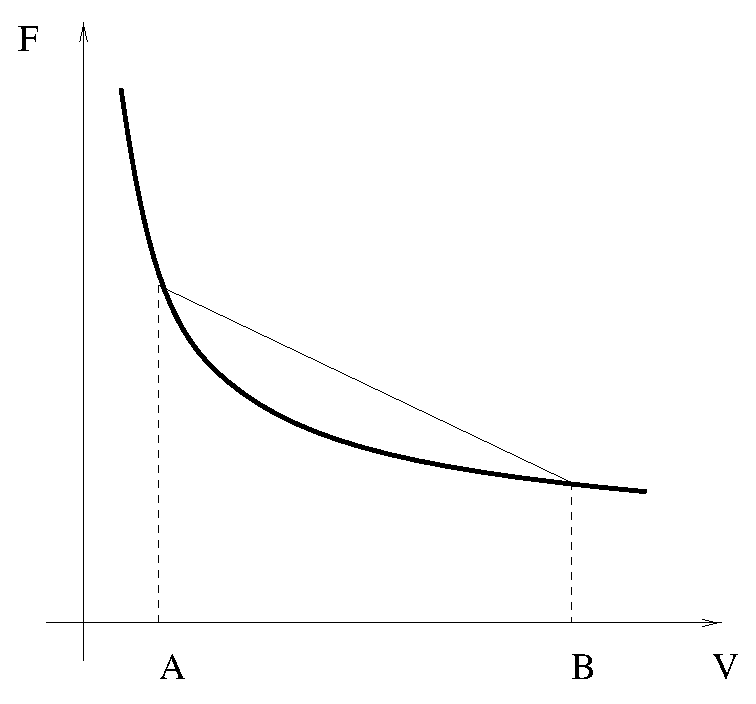
\epsfig{file={../fig/vanavant}}}   
 \caption{Over a critical temperature, energy doesnt present any local
   minimum.} 
 \label{figvanavant}
\end{figure}
\begin{figure}[htb]
 \centerline{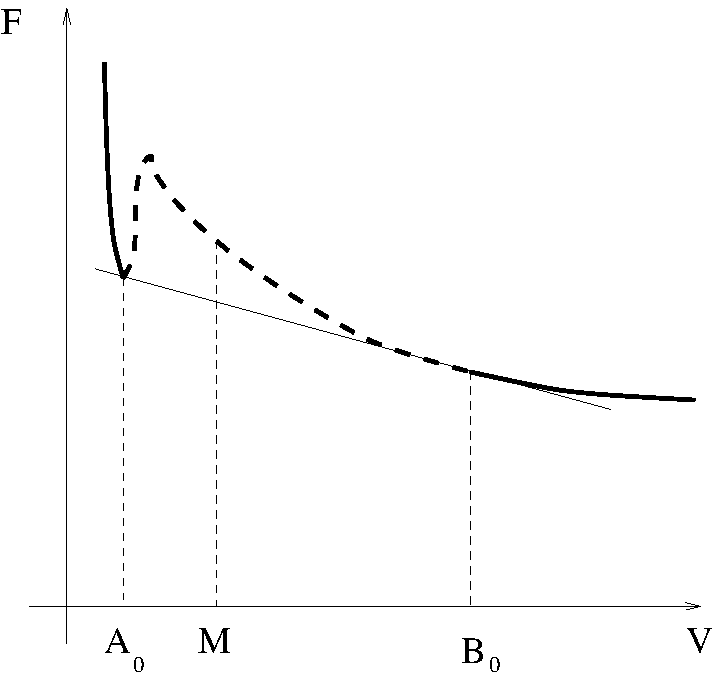
\epsfig{file={../fig/vanapres}}}   
 \caption{Below the critical temperatre, energy presents a local minimum. Two
   phases then appear, characteriszed by points $A_{0}$ et $B_0$.}
 \label{figvanapres}
\end{figure}
When temperature is lower than critical temperature $T_c$, the energy of the
system for a given volume $V_M$ with $V_{A_0}<V_M<V_{B_0}$ is not
$F_v(V_M)$. Indeed, system evolves to a state of lower energy (see figure
\ref{figvanapres}) with energy:  
\begin{equation}
F(V_M)=F_{A_0}+\frac{V_M-V_{A_0}}{V_{B_0}-V_{A_0}}(F_{B_0}-F_{A_0})
\end{equation}
The apparition of a local minimum of $F$ corresponds to the apparition of two
phases.\index{phase transition} 
\section{Ising Model}\label{secmodising}
%%%%%%%%%
In this section, an example of the calculation of a partition function is
presented. The Ising model
\cite{ma:equad:Schuster88,ph:physt:Diu89}
\index{Ising} is a model describing ferromagnetism\index{ferromagnetic}. 
A ferromagnetic  material is constituted by small microscopic domains having a
small magnetic moment. The orientation of those moments being random, the
total magnetic moment is zero. However, below a certain critical temperature
$T_c$, magnetic moments orient themselves along a certain direction, and a non
zero 
total magnetic moment is observed\footnote{%%%%%%%
Ones says that a phase transition occurs.\index{phase transition}
Historically, two sorts of phase transitions are distinguished
\cite{ph:physt:Diu89} 
\begin {enumerate}
\item phase transition of first order (like liquid--vapor transition) whose
  characteristics are:
\begin{enumerate}
\item Coexistence of the various phases.
\item Transition corresponds to a variation of entropy.
\item existence of metastable states.
\end{enumerate}
\item second order phase transition (for instance the
  ferromagnetic--paramagnetic transition) whose characteristics are:
\begin{enumerate}
\item symmetry breaking
\item the entropy S is a continuous function of temperature and of the order
  parameter.
\end{enumerate}
\end{enumerate}
}%%%%%%%%%%%%%%%
. Ising model has been proposed to describe this phenomenom.
It consists in describing each microscopic domain by a moment $S_i$ (that can
be considered as a spin)\index{spin}, the interaction between spins being
described by the following hamiltonian (in the one dimensional case):
\begin{equation}
H=-K\sum S_lS_{l+1}
\end{equation}
partition function of the system is:
\begin{equation}
Z=\sum_{(S_l)}\Pi_{l=0}^{N-1}e^{-KS_lS_{l+1}},
\end{equation}
which can be written as:
\begin{equation}
Z=\sum_{(S_l)}\Pi_{l=0}^{N-1}\mbox{ ch } K +S_lS_{l+1}\mbox{ sh } K.
\end{equation}
It is assumed that $S_l$ can take only two values. Even if the one dimensional
Ising model does not exhibit a phase transition, we present here the
calculation of the partition function in two ways.
$\sum_{(S_l)}$ represents the sum over all possible values of $S_l$, it is
thus, in the same way an integral over a volume is the successive integral
over each variable, the successive sum over the $S_l$'s. Partition function $Z$
can be written as:
\begin{equation}
Z=\sum_{S_1}\dots\sum_{S_n}f(S_1,S_2)f(S_2,S_3)\dots
\end{equation}
with
\begin{equation}
f_{K}(S_i,S_{i+1})=\mbox{ ch } K +S_iS_{i+1}\mbox{ sh } K
\end{equation}
We have:
\begin{equation}
\sum_{S_1}f(S_1,S_2)=2 \mbox{ ch } K.
\end{equation}
Indeed:
\begin{equation}
\sum_{S_1}f(S_1,S_2)=\mbox{ ch } K +S_2 (+1)\mbox{ sh } K + \mbox{ ch } K +S_2 (-1) \mbox{ sh } K.
\end{equation}
Thus, integrating successively over each variable, one obtains:
\begin{equation}\label{eqZisi}
Z=2^{n-1} (\mbox{ ch } K)^{n-1}
\end{equation}

This result can be obtained a powerful calculation method: the {\bf
  renormalization group
  method}\cite{ph:physt:Diu89,ma:equad:Schuster88}
\index{renormalisation group} proposed by  K. Wilson\footnote{Kenneth
  Geddes Wilson received the physics Nobel price in 1982 for the
  method of analysis introduced here.}. 
Consider again the partition function:
\begin{equation}
Z=\sum_{S_1}\dots\sum_{S_n}f_K(S_1,S_2)f_K(S_2,S_3)\dots
\end{equation}
where
\begin{equation}
f_{K}(S_i,S_{i+1})=\mbox{ ch } K +S_iS_{i+1}\mbox{ sh }K
\end{equation}
Grouping terms by two yields to:
\begin{equation}
Z=\sum_{S_1}\dots\sum_{S_n}g(S_1,S_2,S_3).g(S_3,S_4,S_5)\dots
\end{equation}
where
\begin{equation}
g(S_i,S_{i+1},S_{i+2})=(\mbox{ ch } K +S_iS_{i+1}\mbox{ sh }K)(\mbox{ ch } K +S_{i+1}S_{i+2}\mbox{ sh }K)
\end{equation}
This grouping is illustrated in figure \ref{figrenorm}.
\begin{figure}[htb]
 \centerline{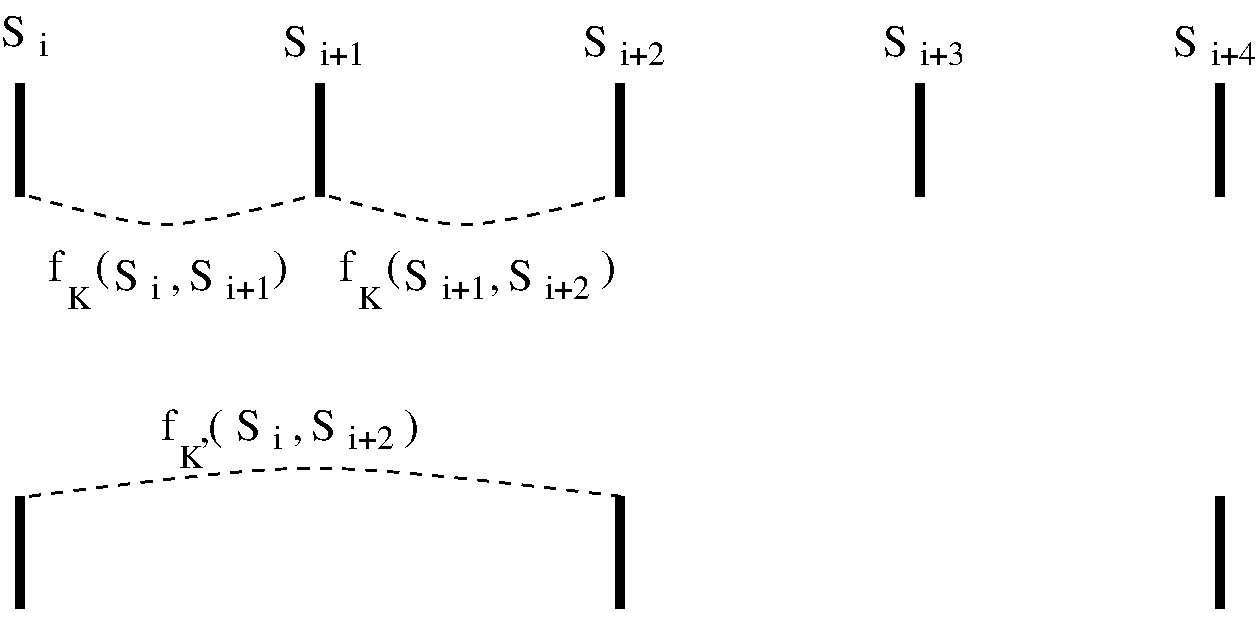
\epsfig{file={../fig/renorm}}}  
\caption{Sum over all possible spin values $S_{i},S_{i+1},S_{i+2}$. The product
$f_K(S_i,S_{i+1})f_K(S_{i+1},S_{i+2})$ is the sum over all possible values of
spins $S_{i}$ and $S_{i+2}$ of a function $f_{K'}(S_{i},S_{i+2})$ deduced from
$f_K$ by a simple change of the value of the parameter
$K$ associated to function $f_K$.} 
 \label{figrenorm}
\end{figure}
Calculation of sum over all possible values of $S_{i+1}$ yields to:
\begin{equation}
\sum_{S_{i+1}}g(S_i,S_{i+1},S_{i+2})=2(\mbox{ ch }^2K+S_{i}S_{i+2}\mbox{ sh }^2K)
\end{equation}
Function $\sum_{S_{i+1}}g(S_i,S_{i+1},S_{i+2})$ can thus be written as a
second function $f_{K'}(S_i,S_{i+2})$ with
\begin{equation}
K'=\mbox{ Arcth }(\mbox{ th }^2K).
\end{equation}
Iterating the process, one obtains a sequence converging towards
the partition function $Z$ defined by equation \ref{eqZisi}.
\section{Spin glasses}\label{secverredespi}
%%%%%%%%%%%%%%%%%%%%%%%%
Assume that a spin glass system \index{spin glass}(see
section{secglassyspin}) has the energy: 
\begin{equation}
H=\sum J_{ij}S_iS_j
\end{equation}
Values of variable $S_i$ are $+1$ if the spin is up or $-1$ if the spin is
down. Coefficient $J_{ij}$ is $+1$ if spins $i$ and $j$ tend to be oriented in
the same direction or $-1$ if spins $i$ and $j$ tend to be oriented in
opposite directions (according to the random position of the atoms carrying
the spins). Energy is noted:
\begin{equation}
H_J=\sum J_{ij}S_iS_j
\end{equation}
where $J$ in $H_J$ denotes the $J_{ij}$ distribution. Partitions function is: 
\begin{equation}
Z_J=\sum_{[s]}e^{-\beta H_J[s]}
\end{equation}
where $[s]$ is a spin configuration. We look for the mean $\bar f$ over
$J_{ij}$ distributions of the energy:
\begin{equation}
\bar f=\sum_JP[J]f_J
\end{equation}
where $P[j]$ is the probability density function of configurations $[J]$, and where $f_J$ is:
\begin{equation}
f_J=-\ln Z_J.
\end{equation}
This way to calculate means is not usual in statistical physics. Mean is done
on the ``chilled'' $J$ variables, that is that they vary slowly with respect
to the $S_i$'s. A more classical mean would consist to $\sum_J
P[J]\sum_{[s]}e^{-\beta H_J[s]}$ (the $J$'s are then ``annealed'' variables).
Consider a system $S_j^n$ compound by  $n$ replicas\index{replica} of the
same system $S_J$. Its partition function $Z_J^n$ is simply:
\begin{equation}
Z_J^n=(Z_J)^n
\end{equation}
Let $f_n$ be the mean over $J$ defined by:
\begin{equation}
f_n=-\frac{1}{n}\ln \sum_J P[J](Z_J)^n
\end{equation}
As:
\begin{equation}
\ln Z=\lim_{n\rightarrow 0}\frac{Z^n-1}{n}
\end{equation}
we have:
\begin{equation}
\lim_{n\rightarrow 0}f_n=\lim_{n\rightarrow 0}\ln (\sum_J P[J][1+n \ln Z_J])
\end{equation}
Using $\sum_JP[J]=1$ and $\ln(1+x)=x+O(x)$ one has:
\begin{equation}
\bar f=\lim_{n\rightarrow 0}f_n.
\end{equation}
By using this trick we have replaced a mean over $\ln Z$ by a mean over $Z^n$;
price to pay is an analytic prolongation in zero. Calculations are then
greatly simplified\cite{ph:sping:Mezard87}.

Calculation of the equilibrium state of a frustrated system can be made by
{\bf simulated annealing method}.\index{simulated annealing} An numerical
implementation can be done using the Metropolis algorithm\index{Metropolis}.
This method can be applied to the travelling salesman problem (see
\cite{ma:compu:Press92}
\index{travelling salesman problem}).
\section{Quantum perfect gases}\label{secgasparfq}
%%%%%%%%%%%%%%%%%%%%%%%%%%%%%%%
\subsection{Introduction}
%%%%%%%%%%%%%%%%%%%%%%%%%
Consider a quantum perfect gas, {\it i. e.}, a system of independent particle
that have to be described using quantum mechanics,
\index{quantum perfect gas}
in equilibrium with a particle reservoir \cite{ph:physt:Diu89} and with a
thermostat. The description adopted is called ``grand--canonical''. It can be
shown that the solution of the entropy maximalization problem (using Lagrange
multipliers method) provides the occupation probability $P_l$ of a state $l$
characterized by an energy $E_l$ an a number of particle $N_l$:
\begin{equation}
P_l=\frac{1}{Z}e^{-\beta E_l+\mu\beta N_l}
\end{equation}
with
\begin{equation}
Z=\sum_le^{-\beta E_l+\mu\beta N_l}
\end{equation}
Assume that the independent particles that constitute the system are in
addition identical undiscernible. State $l$ can then be defined by the datum
of the states $\lambda$ of individual particles. 
\begin{figure}[htb]
 \centerline{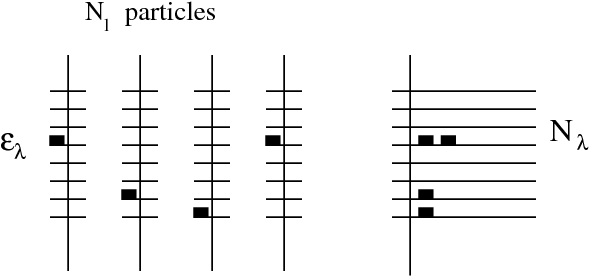
\epsfig{file={../fig/occup}}}   
 \caption{A system whose number of independent particles $N_l$ varies can be
   described by the set of $N_l$ particles energies or, in
   an equivalent way, by numbers $N_\lambda$ of particles at the various energy levels $\epsilon_\lambda$.}
 \label{figoccup}
\end{figure}
Let 
$\epsilon_\lambda$ be the energy of a particle in the state $\lambda$. The
energy of the system in state $l$ is then:
\begin{equation}
E_l=\sum_\lambda N_\lambda \epsilon_\lambda
\end{equation}
where $N_\lambda$ is the number of particles that are in a state of energy
$E_\lambda$. This number is called occupation number of state of
energy\index{occupation number} $E_\lambda$ (see
figure~\ref{figoccup}). Thus:
\begin{equation}
N_l=\sum_\lambda N_\lambda
\end{equation}
Partition function becomes:
\begin{equation}
Z=\Pi_\lambda \xi_\lambda
\end{equation}
with
\begin{equation}
\xi_\lambda=\sum_{N_l}e^{-\beta N_\lambda\epsilon_\lambda+\beta
N_\lambda\mu} 
\end{equation}
The average particles number in the system is given by:
\begin{equation}
\beta \bar N=-\frac{\partial \ln Z}{\partial \mu}
\end{equation}
that can be written:
\begin{equation}
\beta \bar N=\sum_\lambda N_\lambda
\end{equation}
where $N_\lambda$ represents the average occupation number and is defined by
following equality: 
\begin{equation}
\beta \bar N_\lambda=\frac{\partial \ln \xi_\lambda}{\partial \mu}
\end{equation}

\subsection{Fermion gases}
%%%%%%%%%%%%%%%%%%%%%%%%%%%
If particles are fermions\index{fermions}, from Pauli 
principle\index{Pauli principle}, occupation number $N_\lambda$ value can
only be either zero (there is no particle in state with energy
$\epsilon_\lambda$) or one (a unique particle has an energy
$\epsilon_\lambda$). 
The expression of partition function then allows to evaluate the various
thermodynamical  properties of the considered system. An application example of
this formalism is the study of  electrical
properties of {\bf
  semiconductors}\cite{ph:physt:Diu89}
\index{metal}\index{semi-conductor}.
Fermion gases can also be used to model {\bf white dwarfs}
\index{white dwarf}.
A white dwarf is a star \cite{ph:physt:Diu89} very dense: its mass is of the
order of an ordinary star's mass
\index{star}
(as sun), but its radius is
50 to 100 times smaller.
Gravitational pressure implies star contraction. This pressure in an ordinary
star is compensated by thermonuclear reaction that occur in the centre of the
star. But is a white wharf, such reactions do not occur no more. Moreover, one
can show that speed of electrons of the star is very small. As all electrons
can not be is the same state from Pauli principle\footnote{%%%%%
Indeed, the state of an electron in a box is determined by its energy, its
position is not defined in quantum mechanics.}%%%%%%%%
, they thus exert a pressure. This pressure called ``quantum pressure''
compensates gravitational pressure and avoid the star to collapse completely.


\subsection{Boson gases}
%%%%%%%%%%%%%%%%%%%%%%%%%%%
If particles are bosons, from Pauli principle, occupation number $N_\lambda$
can have any positive or zero value:
\begin{equation}
\xi^B_\lambda= \sum_{N_\lambda=0}^{+\infty}e^{-\beta
N_\lambda\epsilon_\lambda+\beta N_\lambda\mu} 
\end{equation}
$\xi^B_\lambda$ is sum of geometrical series of reason:
\begin{equation}
e^{-\beta \epsilon_\lambda+\beta \mu}
\end{equation}
where $\epsilon_\lambda$ is fixed. Series converges if
\begin{equation}
\epsilon_\lambda-\mu>0
\end{equation}
It can be shown\cite{ph:physt:Diu89} that at low temperatures, bosons gather
in the state of lowest energy. This phenomena is called Bose
condensation.\index{Bose condensation} 
\begin{rem}
Photons are bosons whose number is not conserved. This confers them a very
peculiar behaviour: their chemical potential is zero.
\end{rem}


\section{N body problems and kinetic description}\label{desccinet}
%%%%%%%%%%%%%%%%
\subsection{Introduction}
%%%%%%%%%%%%%%%%%%%%%%
In this section we go back to the classical description of systems of
particles already tackled at section~\ref{secdistclassi}. Henceforth, we are
interested in the presence probability of a particle in an elementary volume
of space phase. A short excursion out of the thermodynamical equilibrium is
also proposed with the introduction of the kinetic evolution equations.
Those equations can be used to prove conservations laws of continuous media
mechanics (mass conservation, momentum conservation, energy
conservation,\dots) as it will be shown at next chapter.
\subsection{Gas kinetic theory}
%%%%%%%%%%%%%%
Perfect gas problem can be tackled\index{perfect gas} in the frame of a
kinetic theory\index{kinetic description}. This point of view is much
closer to classical mechanics that statistical physics and has the advantage to
provide more ``intuitive'' interpretation of results.
Consider a system of $N$ particles with the internal energy:
\begin{equation}
U=\sum \frac{1}{2}mv_i^2+V(r_1,\dots,r_N)
\end{equation}
A state of the system is defined by the set of the $r_i,p_i$'s. Probability
for the system to be in the volume of phase space comprised between
hyperplanes  $r_i,p_i$  and $r_i+dr_i,p_i+dp_i$ is:
\begin{equation}
dP=\frac{1}{a}e^{-\beta[\sum \frac{1}{2}mv_i^2+V(r_1,\dots,r_N)]}
\end{equation}
Probability for one particle to have a speed between $v$ and $v+dv$ is
\begin{equation}
dP(v)=\frac{1}{B}e^{-\beta \frac{1}{2}mv^2}dv_xdv_ydv_z
\end{equation}
$B$ is a constant which is determined by the normalization condition $\int dP
=1$. Probability for one particle to have a speed component on the $x$-axis
between $v_x$ and $v_x+dv_x$ is 
\begin{equation}
dP(v_x)=N\sqrt{\frac{m}{2\pi k_BT}}e^{-\beta \frac{1}{2}mv_x^2}dv_x
\end{equation}
The distribution is Gausssian. It is known that:
\begin{equation}
\overline{v_x}=0
\end{equation}
and that
\begin{equation}
\overline{v^2_x}=\frac{k_BT}{m}
\end{equation}
Thus:
\begin{equation}
\overline{\frac{1}{2}mv^2_x}=\frac{1}{2}k_BT
\end{equation}
This results is in agreement with equipartition energy theorem \cite{ph:physt:Diu89}.
Each particle that crosses a surface $\Sigma$ increases of
$mv_z$ the momentum.
In the whole box, the number of molecule that have their speed comprised
between $v_z$ and $v_z+dv_z$ is (see figure \ref{figboite})
\begin{figure}[htb]
 \centerline{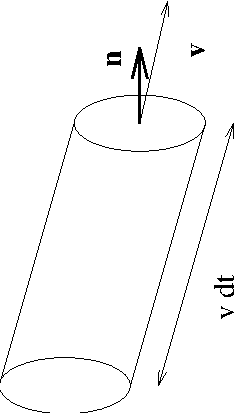
\epsfig{file={../fig/boite}}}   
 \caption{Momentum  transfered by particles in an elementary volume.}
 \label{figboite}
\end{figure}

\begin{equation}
dN=NP(v_z)dv_z
\end{equation}
In the volume $\Delta V$ it is:
\begin{equation}
\Delta(dN)=N\frac{\Delta V}{V}P(v_z)dv_z
\end{equation}
One chooses $\Delta V =s v_z \Delta t$. The increasing of momentum is equal to
the pressure forces power:
\begin{equation}
\int_{-\infty}^{+\infty}m v_z.N\frac{\Delta V}{V}P(v_z)dv_z=p s \Delta t
\end{equation}
so
\begin{equation}
pV=Nk_BT
\end{equation}
We have recovered the perfect gas state equation presented at section
\ref{secgasparfthe}. 
\subsection{Kinetic description}\label{secdesccinet}
%%%%%%%%%%%%%%%%
Let us introduce
\begin{equation}
w(r_1,p_1,\dots,r_n,p_n)dr_1\dots dr_n dp_1\dots dp_n,
\end{equation}
the probability that particle $1$ is the the phase space volume between
hyperplanes $r_1,p_1$ and $r_1 +dr_1,p_1+dp_1$, particle $2$ inthe volume
between hyperplanes $r_2,p_2$ et $r_2 +dr_2,p_2+dp_2$,\dots,
particle $n$ in the volume between hyperplanes $r_n,p_n$ and $r_n
+dr_n,p_n+dp_n$. Since partciles are undiscernable:
\begin{equation}
\frac{1}{N!}w(r_1,p_1,\dots,r_n,p_n)dr_1\dots dr_n dp_1\dots dp_n
\end{equation}
is the probability\footnote{At thermodynamical equilibrium, we have seen
  that$w(r_1,p_1,\dots,r_n,p_n)$ csan be written:
\begin{equation}
w(r_1,p_1,\dots,r_n,p_n)=ae^{-\beta[\sum
\frac{1}{2}mv_i^2+V(r_1,\dots,r_N)]} 
\end{equation}
}%%%%%endfoot
that a particle is inthe volume between hyperplanes $r_1,p_1$ and $r_1
+dr_1,p_1+dp_1$, another particle is in volume between hyperplanes $r_2,p_2$
et $r_2 +dr_2,p_2+dp_2$,\dots, and one last particle in volume between
hyperplanes $r_n,p_n$ and $r_n +dr_n,p_n+dp_n$. We have the normalization
condition: 
\begin{equation}
\int w dr_1\dots dr_n dp_1\dots dp_n=1
\end{equation}
By differentiation:
\begin{equation}
\int \frac{dw}{dt} dr_1\dots dr_n dp_1\dots dp_n+\int w\frac{d
(dr_1\dots dr_n dp_1\dots dp_n)}{dt}=0 
\end{equation}
If the system is hamiltonian\index{hamiltonian system}, volume element is
preserved during the dynamics, and $w$ verify the {\bf Liouville equation}:
\begin{equation}
\frac{dw}{dt}=0.
\end{equation}
Using $r$ and $p$ definitions, this equation becomes:
\begin{equation}
\frac{\partial w}{\partial t}+\{w,H\}=0
\end{equation}
where $H$ is the hamilitonian of the system. One states the following
repartition function:
\begin{equation}
f_1(r,p,t)=\frac{1}{(N-1)!}\int w \Pi_{i=2}^n dr_idp_i
\end{equation}
Intergating Liouville equation yields to:
\begin{equation}
\frac{\partial f_1}{\partial t}=\frac{1}{(N-1)!}\int \{H,w\} \Pi_{i=2}^n dr_idp_i
\end{equation}
and assuming that
\begin{equation}
H=\sum p_i/2m+\sum u_{ij},
\end{equation}
one obtains a hierarchy of equations called
{\bf BBGKY hierarchy}
\index{BBGKY hierachy}
binding the various functions
$f_k(r_1,p_1,\dots,r_k,p_k,t)$ defined by:
\begin{equation}
f_k(r_1,p_1,\dots,r_k,p_k,t)=\frac{1}{(N-k)!}\int w \Pi_{i=k+1}^n
dr_idp_i.
\end{equation} 
To close the infinite hirarchy, various closure conditions can be
considered. The Vlasov closure condition states that $f_2$ can be written: 
\begin{equation}
f_2(r_1,p_1,r_2,p_2)=f_1(r_1,p_1)f_2(r_2,p_2).
\end{equation}
One then obtains the {\bf Vlasov equation}\index{Vlasov equation} :
\begin{equation}
[\frac{\partial}{\partial t}+\frac{p}{m}\frac{\partial}{\partial r}+[F-\frac{\partial \bar{u}}{\partial r}]\frac{\partial }{\partial p}]f_1=0
\end{equation}
where $\bar{u}$ is the mean potential. Vlasov equation can be rewritten by
introducing a effective force $F_e$ describing the forces acting on partciles
in a mean filed approximation:
\begin{equation}\label{eqvlasov}
[\frac{\partial}{\partial t}+\frac{p}{m}\frac{\partial}{\partial r}+F_e\frac{\partial }{\partial p}]f_1=0
\end{equation}
The various momets of Vlasov equation allow to prove the conservation
equations of mechanics of continuous media (see chapter \ref{chapapproxconti}).
\begin{rem}
Another dynamical equation close to Vlasov equation is the {\bf Boltzman
  equation}
\index{Boltzman}
(see \cite{ph:physt:Diu89}. Difference betwen both
equation relies on the way to treat collisions.
\end{rem}

\section{Exercises}
%%%%%%%%%%%%%%%%%%%
\begin{exo}
{\bf Paramagnetism.} Consider a system constituted by $N$ atoms located at
nodes of a lattice. Let $J_i$ be the total kinetic moment of atom number $i$
in its fundamental state. It is known that to such a kinetic moment is
associated a magnetic moment given by:
\begin{equation}
\mu_i=-g\mu_BJ_i
\end{equation}
where $\mu_B$ is the Bohr magneton and $g$ is the Land\'e factor.  $J_i$ can
have only semi integer values.

Assume that the hamiltonian describing the system of $N$ atoms is:
\begin{equation}
H=\sum -\mu_i B_0
\end{equation}
where $B_0$ is the external magnetic field. What sort of particles are the
atoms in this systme, discernables or undiscernables? Find the partition
function of the system.
\end{exo}

\begin{exo}
Study the Ising model at two dimension. Is it possible to envisage a direct
method to calculate $Z$ ? Write a programm allowing to visualize the evolution
of the spins with time, temperature being a parameter.
\end{exo}

\begin{exo}
Consider a gas of independent fermions. Calculate the mean occupation number
$\bar N_\lambda$ of a state $\lambda$. The law you'll obtained is called Fermi
distribution.
\end{exo}

\begin{exo}
Consider a gas of independent bosons. Calculate the mean occupation number
$\bar N_\lambda$ of a state $\lambda$. The law you'll obtained is called Bose
distribution.
\end{exo}

\begin{exo}
Consider a {\bf semi--conductor metal.} Free electrons of the metal are
modelized by a gas of independent fermions. The states are assumed to be
described by a sate density $\rho(\epsilon)$,
$\epsilon$ being the nergy of a state. Give the expression of $\rho(epsilon)$.
Find the expression binding electron number $\bar N$ to chemical
potential. Give the expression of the potential when temperature is zero.
\end{exo}

\chapter{Continuous approximation}\label{chapapproxconti}
%%%%%%%%%%%%%%%%%%%%%%%%%
\section{Introduction}
%%%%%%%%%%%%%%%%%%%%%%
There exist several ways to introduce the matter continuous
approximation. They are different approaches of the averaging over particles
problem. The first approach consists in starting from classical mechanics and
to consider means over elementary volumes called ``fluid elements''.
\begin{figure}[htb]
 \centerline{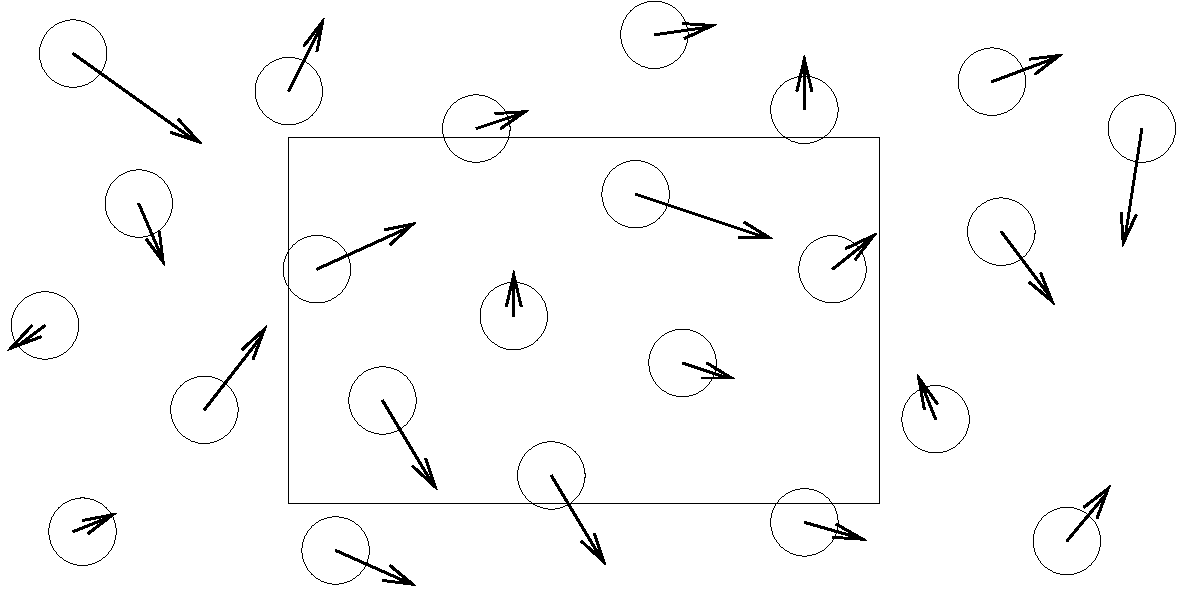
\epsfig{file={../fig/volele}}}   
 \caption{Les moyennes sont faite dans la boite \'el\'ementaire de
volume $d\tau$.}
 \label{figvolele}
\end{figure}
Let us consider an elementary volume $d\tau$ centred at $r$, at time
$t$. Figure \ref{figvolele} illustrates this averaging method. Quantities
associated to continuous approximation are obtained from passage to the limit
when box-size tends to zero.

So the particle density is the extrapolation of the limit when box volume
tends to zero of the ratio of $dn$ (the number of particles in the box) over
$d\tau$ (the volume of the box):
\begin{equation}
n(r,t)=\lim_{d\tau\rightarrow 0}\frac{dn}{d\tau}
\end{equation}
In the same way, mean speed of the medium is defined by:
\begin{equation}
v(r,t)=\lim_{d\tau\rightarrow 0}\frac{dv}{dn}
\end{equation}
where $dv$ is the sum of the speeds of the $dn$ particles being in the box.
\begin{rem}
Such a limit passage is difficult to formalize on mathematical point of view.
It is a sort of ``physicist limit''!
\end{rem}
\begin{rem}
Note that the relation between particles characteristics and mean
characteristics are not always obvious. It can happen that the speed of the
particles are non zero but that their mean is zero. It is the case if
particles undergo thermic agitation (if no convection). But it can also happen
that the temporal averages of individual particle speed are zero, and that in
the same time the speed of the fluid element is non zero! Figure
\ref{figvitnonul} illustrates this remark in the case of the drift
phenomenom\cite{ph:plasm:Chen84}.  
\begin{figure}[htb]
 \centerline{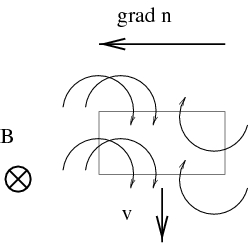
\epsfig{file={../fig/vitnonul}}}   
 \caption{Electrons in a magnetic $B$ field has a uniform rotation
 movement. The time average of each particle deplacement is thus
 zero. However, if there exists a density gradient, the fluid velocity
 in non zero (here directed downwards). It's the ``drift'' phenomenon,
 common in plasma physics.}
 \label{figvitnonul}
\end{figure}
\end{rem}
Another method consists in considering the repartition function for one
particle $f(r,p,t)$ introduced at section
\ref{secdesccinet}. Let us recall that $\frac{1}{n!}f(r,p,t)drdp$ represents
the probability to find at time $t$ a particle in volume of space phase
between $r,p$ and $r+dr,p+dp$. The various fluid quantities are then
introduced as the moments of $f$ with respect to speed. For instance, particle
density is the zeroth order moment of $f$ :
\begin{equation}
n(r,t)=\int f(r,p,t)dp
\end{equation}
that is, the average number of particles in volume a volume $d\tau$ is
\begin{equation}
dn=n(r,t)d\tau.
\end{equation}
Fluid speed is binded to first moment of $f$ :
\begin{equation}
mv(r,t)=\int pf(p,r,t)dp
\end{equation}
The object of this chapter is to present laws governing the dynamics of a
continuous system. In general, those laws can be written as {\bf conservation
  laws}. 
\section{Conservation laws}
%%%%%%%%%
\subsection{Integral form of conservation laws}
%%%%%%%%%%%%%%%%
A conservation law\index{conservation law}
is a balance that can be
applied to every connex domain strictly interior to the considered system and
that is followed in its movement. such a law can be written:
\begin{equation}
\frac{d}{dt}\int_D A_idv+\int_{\partial D} \alpha_{ij}
n_jd\sigma=\int_D a_idv \label{eqcon}
\end{equation}
Symbol $\frac{d}{dt}$ represents the particular derivative (see appendix
\ref{chapretour}). 
$A_i$ is a scalar or tensorial\footnote{%%%%%%%%%%
$A_i$
is the volumic density of quantity ${\cal
A}$ (mass, momentum, energy ...). The subscript $i$ symbolically designs all
the subscripts of the considered tensor.
}%%%%%%%%%%%%%
 function of eulerian variables $x$ and $t$.  $a_i$ is volumic density rate
 provided by the exterior to the system. $\alpha_{ij}$ is the surfacic density
 rate of what is lost by the system through surface bording $D$.
\subsection{Local form of conservation laws}
%%%%%%%%%%%%%%%%
Equation \ref{eqcon} represents the integral form of a conservation law. To
this integral form is associated a local form that is presented now. As
recalled in appendix \ref{chapretour}, we have the following relation:
\begin{equation}
\frac{d}{dt}\int_D A_idv=\int_D \frac{d}{dt} A_idv
\end{equation}
It is also known that:
\begin{equation}
\frac{dA_i}{dt}=\frac{\partial A_i}{\partial t}+(A_iu_j)_{,j}
\end{equation}
Green formula allows to go from the surface integral to the volume
integral:
\begin{equation}
\int_{\partial D} \alpha_{ij}n_jd\sigma=\int_{D} \alpha_{ij,j}dv
\end{equation}
Final equation is thus:
\begin{equation}
\frac{\partial A_i}{\partial t}+(A_iu_j+\alpha_{ij})_{,j}=a_i
\end{equation}
Let us now introduce various conservation laws. 
\section{Matter conservation}
%%%%%%%%%%%%%%%%%%%%%%%%%%%%%%%%%%%%%
Setting $A_i=\rho=\frac{dm}{d\tau}$ in equation \ref{eqcon} one obtains the
matter conservation equation: 
\begin{equation}
\frac{\partial \rho}{\partial t}+\mbox{ div } (\rho u)=0
\end{equation}
$\rho$ is called the volumic mass.
This law can be proved by calculations using elementary fluid volumes. So,
variation of mass $M$ in volume $d\tau$ per time unit is opposed to the
outgoing mass flow:
\begin{equation}
\frac{dM}{dt}=-\int_{d\tau} \rho v dr
\end{equation}
Local form of this equation is thus:
\begin{equation}
\frac{\partial \rho}{\partial t}+\mbox{ div } (\rho u)=0
\end{equation}

But this law can also be proved in calculating the first moment of the Vlasov
equation (see equation \ref{eqvlasov}). Volumic mass is then defined as the
zeroth order moment of the repartition function times mass $m$ of one particle:
\begin{equation}
\rho=m\int dpf(r,p,t)
\end{equation}
Taking the first moment of Vlasov equation, it yields:
\begin{equation}
\frac{\partial \rho}{\partial t}+\nabla (\rho v)=0
\end{equation}
Charge conservation equation is completely similar to mass conservation
equation:
\begin{equation}
\frac{\partial \rho}{\partial t}+\mbox{ div }{j}=0
\end{equation}
where here $\rho$ is the volumic charge and  $j$ the electrical current
density: 
\begin{equation}
j=\rho v
\end{equation}
Flow of $j$ trough an open surface $S$ is usually called electrical current
going through surface $S$.

\section{Momentum conservation}
%%%%%%%%%%%%%%
We assume here that external forces are described by $f$ and that internal
strains are described by tensor $\tau_{ij}$.
\begin{equation}
\frac{d}{dt}\int_D \rho u_idv+\int_{\partial D} \tau_{ij}
n_jd\sigma=\int_D f_idv 
\end{equation}
This integral equation corresponds to the applying of Newton's law of
motion\index{momentum} over the elementary fluid volume as shown by
figure 
\ref{figconsp}. 
\begin{figure}[htb]
 \centerline{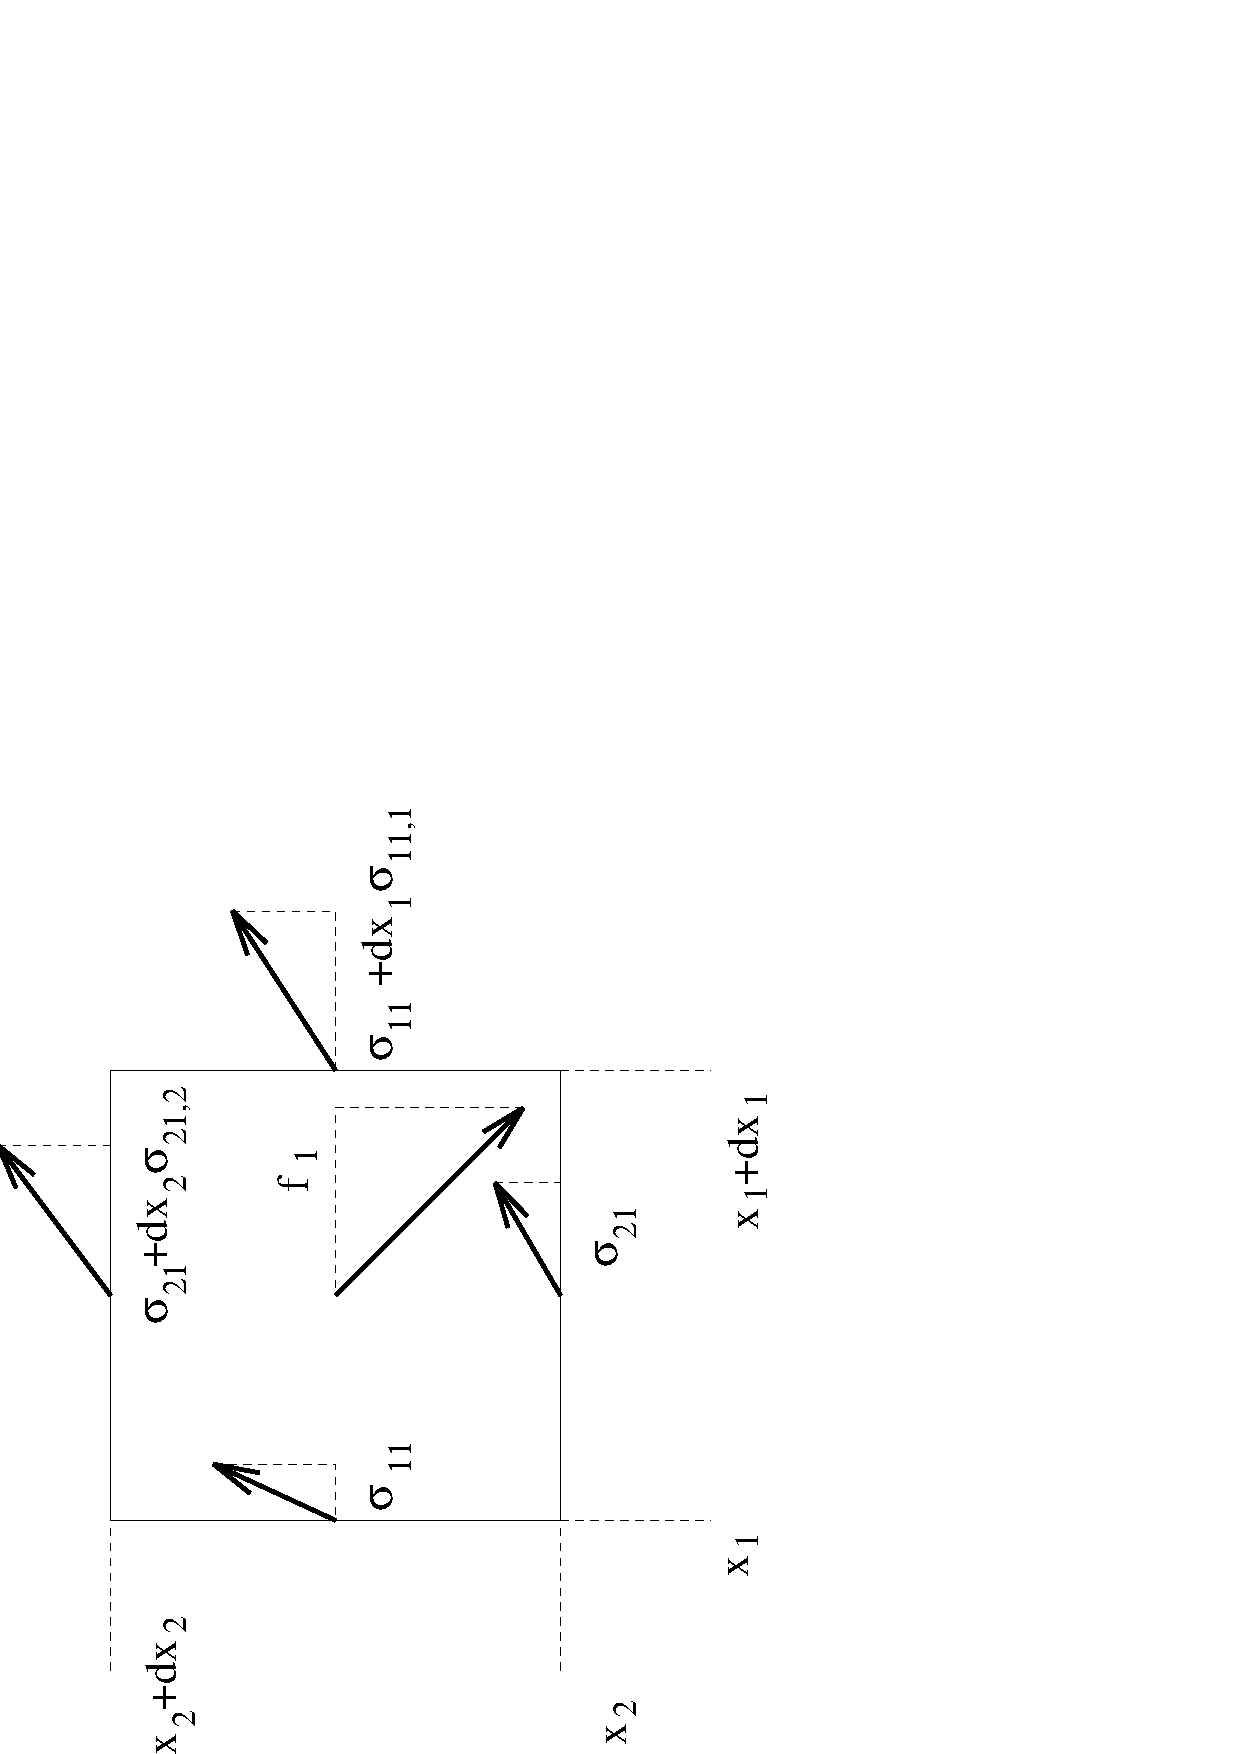
\epsfig{file={../fig/consp}}}   
 \caption{Momentum conservation law corresponds to the application of
   Newton's law of motion to an elementary fluid volume.}
 \label{figconsp}
\end{figure}
Partial differential equation associated to this integral equation is:
\begin{equation}
\frac{\partial}{\partial t}(\rho u_i)+(\rho u_i u_j)_{,j}+\tau_{ij,j}=f_i
\end{equation}
Using continuity equation yields to:
\begin{equation}
\rho(\frac{\partial}{\partial t}u_i+u_j u_{i,j})+\tau_{ij,j}=f_i
\end{equation}

\begin{rem}
Momentum conservation equation can be proved taking the first moment of
Vlasov equation. Fluid momentum $\bar p$ is then related to repartition
function by the following equality:
\begin{equation}
\bar p=\int p dp f(r,p,t)
\end{equation}
\end{rem}
Later on, fluid momentum is simply designated by $p$.
\section{Virtual powers principle}\label{secpuisvirtu}
%%%%%%%%%%%%%%%%%
\subsection{Principle statement}
%%%%%%%%%
Momentum conservation has been introduced by using averages over particles of
quantities associated to those particles. Distant forces have been modelized
by force densities $f_i$, internal strains by a second order tensor
$\tau_{ij}$,\dots This point of view is directly related to the
Newton's law of motion. The dual point of view is presented here:
strains are 
described by the means of movement they permit\cite{ma:equad:Dautray1}).
This way corresponds to our day to day experience
\begin{itemize}
\item to know if a wallet is heavy, one lifts it up.
\item to appreciate the tension of a string, one moves it aside from its
  equilibrium position.
\item pushing a car can tell us if the brake is on.
\end{itemize}
Strains are now evaluated by their effects coming from a displacement or
deformation.  
This point of view is interesting because it allows to defines strains when
they are bad defined in the first point of view, like for frictions or binding
strains. Freedom in modelization is kept very large because the modelizer can
always choose the size of the virtual movements to be allowed. let us precise
those ideas in stating the principle.
\begin{prin}
Virtual power of acceleration quantities is equal to the sum of the virtual
powers of all strains applied to the system, external strains, as well as
internal strains:
\begin{equation}
\int \rho \gamma_i \hat{u}_i
d\tau=P^{int}+P^{ext}_{dist}+P^{ext}_{contact} 
\end{equation}
where $P^{int}$ represents power of internal strains, $P^{ext}_{dist}$, distant
external strains, $P^{ext}_{contact}$ contact external strains.
\end{prin}
At section \ref{sepripuiva} it is shown how a partial differential equation
system can be reduced to a variational system: this can be used to show that
Newton's law of motion and virtual powers principle are dual forms of
a same physical law.


Powers are defined by giving spaces $A$ and $E$ where $A$ is the affine space
attached to $E$:
\begin{equation}
\begin{array}{llll}
P:&L(A,E)&\longrightarrow &R\\
  &u(r)&\longrightarrow &P(u(r))
\end{array}
\end{equation}
At section \ref{seccasflu} we will consider an example that shows the power of
the virtual powers point of view.
\subsection{Virtual powers and local equation}\label{sepripuiva}
%%%%%%%%%%
A connection between local formulation (partial derivative equation or PDE)
and virtual powers principle (variational form of the PDE problem considered)
is presented on an example. Consider the problem:
\begin{prob}
Find $u$ such that:
\begin{equation}
\partial_j\sigma_{i,j}(u)+f_i=0 \mbox{ in } \Omega
\end{equation}
\begin{equation}
u_i=0 \mbox{ on } \Gamma_1
\end{equation}
\begin{equation}
\sigma_{i,j}(u)n_j=0 \mbox{ on } \Gamma_2
\end{equation}
with $\Gamma_1\cup\Gamma_2=\partial\Omega$.
\end{prob}
Let us introduce the bilinear form:
\begin{equation}
a(u,v)=\int_\Omega \sigma_{i,j}(u)\epsilon_{i,j}(v)dx
\end{equation}
and the linear form: 
\begin{equation}
L(v)=\int_\Omega
f_iv_idx+\int_{\Gamma_1}g_iv_idx
\end{equation}
it can be shown that there exist a space $V$ such that there exist a unique
solution $u$ of
\begin{equation}
\forall v\in V, a(u,v)=L(v)
\end{equation}
$a(u,v)$ represents the deformation's work of the elastic solid
\index{virtual power}
\index{elasticity}
corresponding to virtual displacement $v$ from position $u$.
$L(v)$ represents the work of the external forces for the virtual displacement
$v$. The virtual powers principle can thus be considered as a consequence of
the great conservation laws:
\begin{prin}{\bf Virtual powers principle (static case):}
Actual displacement $u$ is the displacement cinematically admissible such that
the deformation's work of the elastic solid corresponding to the virtual
displacement $v$ is equal to the work of the external forces, for any virtual displacement
$v$ cinematically admissible.
\end{prin}
Moreover, as $a(.,.)$ is symmetrical, solution $u$ is also the minimum of
\begin{equation}
J(v)=\frac{1}{2}\int_\Omega
\sigma_{i,j}(v)\epsilon_{i,j}(v)dx-(\int_\Omega 
f_iv_idx+\int_{\Gamma_1}g_iv_idx) 
\end{equation}
$J(v)$ is the potential energy of the deformed solid,
$\frac{1}{2}\int_\Omega \sigma_{i,j}(v)\epsilon_{i,j}(v)dx$ is the deformation
energy. $-(\int_\Omega
f_iv_idx+\int_{\Gamma_1}g_iv_idx)$ is the potential energy of the external
forces. This result \cite{ma:equad:Dautray1} can be stated
as follows:
\begin{prin}
The actual displacement $u$ is the displacement among all the admissible
displacement $v$ that minimizes the potential energy $J(v)$.
\end{prin}

\subsection{Case of fluids}\label{seccasflu}
%%%%%%%%%%
Consider for instance a fluid \cite{ma:equad:Dautray1}.  Assume that the power
of the internal strains can be described by integral:
\begin{equation}
P^{int}=\int (K_i\hat{u}_i+K_{ij}\hat{u}_{i,j})dx
\end{equation}
where $u_{i,j}$ designs the derivative of $u_i$ with respect to coordinate
$j$. The proposed theory is called a first gradient theory.
\begin{rem}
The step of the expression of the power as a function of the speed field $u$
is the key step for modelization. A large freedom is left to the
modelizator. Powers being scalars, they can be obtained by contraction of
tensors (see appendix \ref{chaptens}) using the speed vector field $u_i$ as
well as its derivatives. method to obtain intern energies in generalized
elasticity is similar (see section \ref{secelastigene}).
\end{rem}
Denoting $a$ and $s$ the antisymmetric and symmetric [art of the considered
tensors yields to:\index{tensor} : 
\begin{equation}
P^{int}=\int
(K_i\hat{u}_i+K^{s}_{ij}\hat{u}^{s}_{i,j}+K^{a}_{ij}\hat{u}^{a}_{i,j})dx
\end{equation}
where it has been noted that cross products of symmetric and antisymmetric
tensors are zero\footnote{%%%%%%%%
That is:
$(a_{ij}+a_{ji})(b_{ij}-b_{ji})=0$.
}%%%%%%%%%
. Choosing the uniformly translating reference frame, it can be shown that term
$K_i$ has to be zero:
\begin{equation}
K_i=0
\end{equation}
Antisymmetric tensor is zero because movement is rigidifying:
\begin{equation}
K^{a}_{ij}=0.
\end{equation}
Finally, the expression of the internal strains is:\index{strains}
\begin{equation}
P^{int}=\int (K^{s}_{ij}\hat{u}^{s}_{i,j})dx
\end{equation}
$K^{s}_{ij}$ is called strain tensor since it describes the internal
deformation strains. The external strains power is modelized by:
\begin{equation}
P^{ext}_{dist}=\int (f_i\hat{u}_i+F_{ij}\hat{u}_{i,j})dx
\end{equation}
Symmetric part of $F_{ij}$ can be interpreted as the volumic double--force
density and its antisymmetrical part as volumic couple density. Contact
strains are modelized by: 
\begin{equation}
P^{ext}_{contact}=\int (T_i\hat{u}_i+T_{ij}\hat{u}_{i,j})dx
\end{equation}
Finally the PDE problem to solve is:
\begin{equation}
f_i+\tau_{ij,j}=\rho \gamma_i \mbox{ in } V
\end{equation}
where $\tau_{ij}=K_{ij}^s-F_{ij}$
\begin{equation}
T_i=\tau_{ij}n_j, \mbox{ sur } \partial V
\end{equation}
\begin{equation}
T_{ij}=0, \mbox{ sur } \partial V
\end{equation}
\subsection{Stress-deformation tensor}
%%%%%%%%%%%%%
The next step is to modelize the internal strains. that is to explicit the
dependence of tensors $K_{ij}$ as functions of $u_i$.
This problem is treated at chapter \ref{parenergint}.
Let us give here two examples of approach of this problem.
\begin{exmp}
For a perfect gas, pressure force work on a system of volume $V$ is:
\begin{equation}
\delta W=-pdV.
\end{equation}
The state equation (deduced from a microscopic theory)
\begin{equation}
pV=nk_BT
\end{equation}
is used to bind the strain $p$ to the deformation $dV$.
\end{exmp}
\begin{exmp}
The elasticity theory (see chapter \ref{parenergint}) allows to bind the
strain tensor $\tau_{ij}$ to the deformation tensor $\epsilon_{ij}$ 
\end{exmp}
\section[Energy conservation]{Energy conservation and first principle of thermodynamics}\label{secpremierprinci}
%%%%%%%%%%%%%%%%%%%%%%%%%%%%%%%%%%%%%%%%%%%%%%%%%%%%
\subsection{Statement of first principle}
%%%%%%%%%%%%%%%%%%%%%%
Energy conservation law corresponds to the first principle of thermodynamics
\cite{ph:fluid:Truesdell66,ph:fluid:Germain80,ph:elect:Petit89}.
\index{first principle of thermodynamics}

\begin{defn}
Let $S$ be a macroscopic system relaxing in $R_0$. Internal energy $U$ is the
sum of kinetic energy of all the particle $E_{cm}$ and their total interaction
potential energy $E_p$:
\begin{equation}
U=E_{cm}+E_p
\end{equation}
\end{defn}
\begin{defn}
Let a macroscopic system moving with respect to $R$. It has a macroscopic
kinetic energy $E_c$. The total energy $E_{tot}$ is the sum of the kinetic
energy $E_c$ and the internal energy $U$.
\index{internal energy}
\begin{equation}
E_{tot}=E_c+U
\end{equation}
\end{defn}
\begin{prin}
Internal energy $U$ is a state function\footnote{%%%%%%
That means that an elementary variation $dU$ is a total differential.
}%%%%%
. Total energy
$E_{tot}$ can vary only by exchanges with the exterior.
\end{prin}
\begin{prin}
At each time, particulaire derivative (see example \ref{exmppartder}) of the
total energy $E_{tot}$ is the sum of {\bf external} strains power $P_e$ and of
the heat $\dot Q$
\index{heat}
received by the system.
\end{prin}
\begin{equation}
\frac{dE_{tot}}{dt}=P_e+\dot Q
\end{equation}
This implies:
\begin{thm}
For a closed system, $dE_{tot}=\delta W_{e}+\delta Q$
\end{thm}
\begin{thm}
If macroscopic kinetic energy is zero then:
\begin{equation}
dU=\delta W+\delta Q
\end{equation}
\end{thm}
\begin{rem}
Energy conservation can also be obtained taking the third moment of Vlasov
equation (see equation \ref{eqvlasov}).
\end{rem}
\subsection{Consequences of first principle}
%%%%%%%%%%%%%%%%%%%
The fact that $U$ is a state function implies that:
\begin{itemize}
\item Variation of $U$ does not depend on the followed path, that is variation
  of $U$ depends only on the initial and final states.
\item $dU$ is a total differential that that Schwarz theorem can be
  applied. If $U$ is a function of two variables $x$ and $y$ then:
\begin{equation}
\frac{\partial^2 U}{\partial x\partial y}=\frac{\partial^2 U}{\partial
y\partial x} 
\end{equation}
\end{itemize}
Let us precise the relation between dynamics and first principle of
thermodynamics. From the kinetic energy theorem:
\begin{equation}
\frac{dE_c}{dt}=P_e+P_i
\end{equation}
so that energy conservation can also be written:
\begin{equation}\label{eint}
\frac{dU}{dt}=\dot Q-P_i
\end{equation}
System modelization consists in evaluating $E_c$,
$P_e$ and $P_i$. Power $P_i$ by relation
\ref{eint} is associated to the $U$ modelization.
\section{Second principle of thermodynamics}
%%%%%%%%%%%%%%%%%%%%%%%%%
\subsection{Second principle statement}
%%%%%%%%%%%%%%%%%%%%%%%%%%%%%%%%%%%%%%%%%%
Second principle of thermodynamics\
index{second principle of thermodynamics}
is the macroscopic version of maximum entropy fundamental
principle of statistical physics. Before stating second principle, let us
introduce the thermostat notion:
\begin{defn}
S system $\tau$ is a thermostat for a system $\cal S$ if its microcanonical
temperature is practically independent on the total energy $E$ of system $\cal
S$. 
\end{defn}
We thus have:
\begin{equation}
\frac {\partial S^*_{\tau}}{\partial E_{\tau}}(E_{tot}-E)=\frac
{\partial S^*}{\partial E_{\tau}}(E_{tot})
\end{equation}
so
\begin{equation}
S^*_{\tau}(E_{tot}-E)=S^*(E_{tot})-\beta k E
\end{equation}
\begin{postulat} {\bf Second principle.} For any system, there exists a state
  function called entropy and noted $S$. Its is an extensive quantity whose
  variation can have two causes:
\begin{itemize}
\item heat or matter exchanges with the exterior.
\item internal modifications of the system.
\end{itemize}
Moreover, if for an infinitesimal transformation, one has:
\begin{equation}
dS=\delta_eS+\delta_iS
\end{equation}
then
\begin{equation}
\delta_iS \geq 0
\end{equation}
and
\begin{equation}
\delta_eS =\frac{\delta Q}{T_e}
\end{equation}
\end{postulat}
\begin{rem} Second principle does correspond to the maximum entropy criteria
  of statistical physics. Indeed, an internal transformation is always due to
  a constraint relaxing\footnote{%%%%%%%%%%%%%%%%%%
here are two examples of internal transformation:
\begin{itemize}
\item {\bf Diffusion process.} 
\item {\bf Adiabatic compression.}
Consider a box whose volume is adiabatically decreased. This transformation
can be seen as an adiabatic relaxing of a spring that was compressed at initial
time.
\end{itemize}}%%%%%%%%%%%%%%%%%%%%%%%%%%%%%%%%%%%%
\end{rem}
\begin{rem}
In general, $ \delta_iS $ can not be reached directly. Following equalities
are used to calculate it:
\begin{eqnarray}
dS_r&=&\frac{\delta Q}{T}\\
\delta S_e&=&\frac{\delta Q}{T_e}
\end{eqnarray}
\end{rem}

\subsection{Applications}
%%%%%%%
Here are two examples of application of second principle:
\begin{exmp}
Consider a cylinder by a piston of mass $m$, surface $A$, vertically mobile on
which a sand pile of mass $M$ is put. This cylinder contains perfect gas at
pressure $P_1=P_e+(M+m)g/A$, ($P_e$ is the external pressure) and at
temperature $T_1=T_e$ ($T_e$ is the external temperature). Sand is removed at
one go. Final state is defined by a temperature $T_2=T_e$, a pressure
$p_2=P_e+mg/A$, a number of gas molecules $n_2=n_1$. Work done during this
irreversible transformation $i$ is:
\begin{equation}
W_i=-P_2\int dV=-P_2(V_2-V_1)
\end{equation}
Consider a reversible transform $r$ with the same initial and final states, but
where sand is removed quasi statically. Work done during this transform is:
\begin{equation}
W_r=-\int_{V_1}^{V_2}pdV =-nRT\int_{V_1}^{V_2}\frac{dV}{V}=
-nRTln(\frac{V_2}{V_1}) 
\end{equation}
from the second principle of thermodynamics, the entropy variation during
transformations $i$ and $r$ are equal:
\begin{equation}
\Delta S_i=\Delta S_r.
\end{equation}
Now, using again second principle:
\begin{equation}
\Delta S_r=\frac{\delta Q_r}{T}
\end{equation}
and
\begin{equation}
\Delta S_i=\Delta S_{i,int}+\Delta S_{i,ext}
\end{equation}
with
\begin{equation}
\Delta S_{i,ext}=\frac{\delta Q_i}{T}.
\end{equation}
So
\begin{equation}
T\Delta S_{i,int}=\delta Q_r-\delta Q_i
\end{equation}    
Applying the first principle of thermodynamics:
\begin{equation}
\Delta U_i=\Delta U_r
\end{equation}
so
\begin{equation}
T\Delta S_{i,int}=W_i-W_r
\end{equation}
and finally:
$$
T\Delta S_{i,int}=-P_2\int
dV=-P_2(V_2-V_1)\int_{V_1}^{V_2}pdV =
-nRT\int_{V_1}^{V_2}\frac{dV}{V}=-nRTln(\frac{V_2}{V_1}) 
$$
\end{exmp}
\begin{exmp}
At section \ref{secrelacont}, we have proved relations providing the most
probable quantities encountered when a constraint ``fixed quantity'' is relaxed
to a constraint ``quantity free to fluctuate around a fixed mean''. This
result can be recovered using the second principle. During a transformation at
$p$ and $T$ constant (even an irreversible transformation):
\begin{equation}
\Delta G(p,T,n_1,n_2)=\Delta Q -T_e\Delta S
\end{equation}
Using second principle:
\begin{equation}
\Delta G=-T_e\Delta S_{int}
\end{equation}
with $\Delta S_{int}\geq 0$. At equilibrium\footnote{%%%%%%%%%%%%%%
We are recovering the equivalence between the physical statistics general
postulate ``Entropy is maximum at equilibrium'' and the second principle of
thermodynamics. In thermodynamics, one says that $G(T,p,n_i)$ is minimal for
$T$ and $p$ fixed}%%%%%%%%%%%%%%%%%%%%%%%%%%%
system's state is defined by $\Delta G=0$, so
\begin{equation}
\sum\mu_i dn_i=0
\end{equation}
where $\mu_i$is the chemical potential of species $i$. 
\end{exmp}


\section{Exercises}
%%%%%%%%%%%%%%%%%%%
\begin{exo}
Give the equations governing the dynamics of a plate (negligible thickness)
from powers taking into account the gradient of the speeds (first gradient
theory). Compare with a approach starting form conservation laws.
\end{exo}

\begin{exo}
Same question as previous problem, but with a rope clamped between two walls. 
\end{exo}

\begin{exo}\label{exoplasmapert}
A plasma\index{plasma} is a set of charged particles, electrons and ions. A
classical model of plasma is the ``two fluid model'': the system is described
by two sets of functions density, speed, and pressure, one for each type of
particles, electrons and ions: set $n_e, v_e, p_e$ characterizes the electrons
and set $n_i, v_i, p_i$ characterizes the ions. The momentum conservation
equation for the electrons is:
\begin{equation}\label{me}
n_e m_e(\frac{\partial v_e}{\partial t}+({v}_e.\nabla
v_e))=en_e\nabla \phi - e n_e v_e \wedge B -\nabla p_e
\end{equation}
The momentum conservation equation for the ions is:
\begin{equation}\label{mi}
n_i m_i(\frac{\partial v_i}{\partial t}+({v}_i.\nabla v_i))=-en_i\nabla \phi + en_i v_i \wedge B -\nabla p_i.
\end{equation}
Solve this non linear problem (find solution $n_i(\vec r,t)$) assuming:
\begin{itemize}
\item $B$ field is directed along direction $z$ and so defines parallel
  direction and a perpendicular direction (the plane perpendicular to the $B$
  field). 
\item speeds can be written $v_a=\tilde{v}_a+v_a^0$ with $v_i^0=0$ and
  $v_e^0=-\frac{k_B T_e \nabla_x n^0}{e B n^0} e_{\theta}$. 
\item $E_\perp$ field can be written: $E_\perp=0+\tilde{E}_\perp$.
\item densities can be written $n_a=n_0+\tilde{n}_a$. Plasma satisfies the
  quasi--neutrality condition\index{quasi-neutrality} :
  $\tilde{n}_e=\tilde{n}_i=\tilde{n}$. 
\item gases are considered perfect: $p_a=n_ak_BT_a$.
\item $T_e$, $T_i$ have the values they have at equilibrium.
\end{itemize}

\end{exo}

\chapter{Energy in continuous media}\label{chapenermilcon}\label{parenergint}
%%%%%%%%%%%%%%%%%%%%%%%%%%%%%%%
\section{Introduction}
%%%%%%%%%%%%%%%%%%%%%%
The first principle of thermodynamics (see section \ref{secpremierprinci})
allows to bind the internal energy variation to the internal strains power
\index{strains}:
\begin{equation}
\frac{dU}{dt}=\dot Q -P_i
\end{equation}
if the heat flow is assumed to be zero, the internal energy variation is:
\begin{equation}
dU=-P_i dt
\end{equation}
This relation allows to bind mechanical strains ($P_i$ term) to
system's thermodynamical properties ($dU$ term). When modelizing a system some
``thermodynamical'' variables $X$ are chosen. They can be scalars $x$,
vectors $x_i$, tensors $x_{ij}$, \dots {\bf Differential $dU$} can be
naturally expressed using those thermodynamical variables $X$ by using a
relation that can be symbolically written:
\begin{equation}
dU=FdX
\end{equation}
where $F$ is the conjugated\footnote{%%%%%%%%
This is
the same duality relation noticed between strains and speeds and their
gradients when dealing with powers.}%%%%%%%
 thermodynamical variable of variable
$X$. In general it is looked for {\bf expressing $F$ as a function of $X$}.
\begin{rem}
If $X$ is a scalar $x$, the energy differential is:
\begin{equation}
dU=f.dx
\end{equation}
If $X$ is a vector $x_i$, the energy differential is:
\begin{equation}
dU=f_idx_i
\end{equation}
Si $X$ is a tensor $x_{ij}$, the energy differential is:
\begin{equation}
dU=f_{ij}dx_{ij}
\end{equation}
\end{rem}
\begin{rem}
If a displacement $x$, is considered as thermodynamical variable, then the
conjugated variable $f$ has the dimension of a force.
\end{rem}
\begin{rem}
One can go from a description using variable $X$ as thermodynamical variable
to a description using the conjugated variable $F$ of $X$ as thermodynamical
variables by using a 
{\bf Legendre transformation} (see section \ref{secmaxient} 
and \cite{ph:physt:Diu89}).
\index{Legendre transformation}
The internal
energy $U$ is then transformed to another function called depending on the
case, enthalpy, free energy, etc\dots
\end{rem}
The next step is, using physical arguments, to find an {\bf expression of the
internal energy $U(X)$}
\index{internal energy}
as a function of
thermodynamical variables $X$. Relation $F(X)$ is obtained by differentiating
$U$ with respect to $X$, symbolically:
\begin{equation}
F(X)=\frac{\partial U}{\partial X}
\end{equation}
In this chapter several examples of this modelization approach are presented.


\section{Electromagnetic energy}\label{secenergemag2}
%%%%%%%%%%%%%%%%%%%%
\subsection{Introduction}
%%%%%%%%%%%%%%%%%%%%
At chapter \ref{chapelectromag}, it has been postulated that the
electromagnetic power given to a volume is the outgoing flow of the Poynting
vector.
\index{Poynting vector}
If currents are zero, the energy density
given to the system is:
\begin{equation}
dU=HdB+EdD
\end{equation}

\subsection{Multipolar distribution}
%%%%%%%%%%%
It has been seen at section \ref{secenergemag} that energy for a volumic
charge distribution $\rho$ is
\index{multipole}  
\begin{equation}
U=\int \rho V d\tau
\end{equation}
where $V$ is the electrical potential. Here are the energy expression for
common charge distributions:
\begin{itemize}
\item for a point charge $q$, potential energy is: $U=qV(0)$.
\item for a dipole
\index{dipole}
$P_i$ potential energy is: $U=\int V\mbox{ div }(P_i\delta)=\partial_i V.P_i$. 
\item for a quadripole $Q_{i,j}$ potential energy is: $U=\int
  V(\partial_i\partial_jQ_{i,j}\delta)=\partial_i\partial_j V.Q_{i,j}$. 
\end{itemize}
Consider a physical system constituted by a set of point charges $q_n$
located at $r_n$. Those charges can be for instance the electrons of an atom
or a molecule. let us place this system in an external static electric field
associated to an electrical potential $U_e$. Using linearity of Maxwell
equations, potential $U_t(r)$ felt at position $r$ is the sum of external
potential $U_e(r)$ and potential $U_c(r)$ created by the point charges. 
The expression of total potential energy of the system is:
\begin{equation}
U_t=\sum q_n (V_c(r_n)+V_e(r_n))
\end{equation}
In an atom,\index{atom} term associated to $V_c$ is supposed to be dominant
because of the low small value of $r_n-r_m$. This term is used to compute
atomic states. Second term is then considered as a perturbation. Let us look
for the expression of the second term $U_e=\sum q_n V_e(r_n)$. For that, let
us expand potential around $r=0$ position: 
\begin{equation}
U_e=\sum q_n V_e(r_n)=\sum q_n
(U(0) +x_i^n\partial_i(U)+
\frac{1}{2}x_i^nx_j^n\partial_i\partial_j(U)+\dots)
\end{equation}
where $x_i^n$ labels position vector of charge number $n$. 
This sum can be written as:
\begin{equation}
U_e=\sum q_n U(0)+\sum q_nx_i^n\partial_i(U)+\frac{1}{2}\sum
q_nx_i^nx_j^n\partial_i\partial_j(U)+\dots 
\end{equation}
the reader recognizes energies associated to multipoles.

\begin{rem} In quantum mechanics, passage laws from classical to quantum
  mechanics allow to define tensorial operators (see chapter
\ref{chapgroupes}) associated to multipolar momenta. 
\end{rem}
\subsection{Field in matter}\label{secchampdslamat}
%%%%%%%%%%%%%%%%%%%%%%%%%%%%%%%
In vacuum electromagnetism, the following constitutive relation is exact:
\begin{equation}\label{eqmaxwvideE}
D=\epsilon_0E
\end{equation}
\begin{equation}\label{eqmaxwvideB}
H=\frac{B}{\mu_0}
\end{equation}
Those relations are included in Maxwell equations. Internal electrical energy
variation is:
\begin{equation}
dU=EdD
\end{equation}
or, by using a Legendre transform and choosing the thermodynamical variable
$E$: 
\begin{equation}
dF=DdE
\end{equation}
We propose to treat here the problem of the modelization of the function
$D(E)$. In other words, we look for the medium constitutive relation. This
problem can be treated in two different ways. The first way is to propose {\it
  a priori} a relation $D(E)$ depending on the physical phenomena to
describe. For instance, experimental measurements show that $D$ is
proportional to $E$. So the constitutive relation adopted is:
\begin{equation}
D=\chi E
\end{equation}
Another point of view consist in starting from a microscopic level, that is to
modelize the material as a charge distribution is vacuum. Maxwell equations in
vacuum 
\ref{eqmaxwvideE} and \ref{eqmaxwvideB} can then be used to get a macroscopic
model. Let us illustrate the first point of view by some examples:
\begin{exmp}
If one impose a relation of the following type:
\begin{equation}
D_i=\epsilon_{ij}E_j
\end{equation}
then medium is called {\bf dielectric}.\index{dielectric}
The expression of the energy is:
\begin{equation}
F=F_0+\epsilon_{ij}E_iE_j
\end{equation}
\end{exmp}

\begin{exmp}
In the {\bf linear response } theory \index{linear response}, $D_i$ at time $t$ is supposed to depend not only on the values of
$E$ at the same time $t$, but also on values of $E$ at times anteriors. This
dependence is assumed to be linear:
\begin{equation}
D_i(t)=\epsilon_{ij}*E_j
\end{equation}
where $*$ means time convolution.
\end{exmp}

\begin{exmp}
To treat the {\bf optical activity}\cite{ph:elect:LandauEle}, a
tensor
\index{optical activity}
$a_{ijk}$ such that:
\begin{equation}
D_i=\epsilon_{ij}E_j+a_{ijk}E_{j,k}
\end{equation}
is introduced. Note that this law is still linear but that $D_i$ depends on the
gradient of $E_i$.
\end{exmp}
The second point of view is now illustrated by the following two examples:
\begin{exmp}
{\bf A simple model for the susceptibility:}
\index{susceptibility}
An elementary electric dipole located at $r_0$ can be modelized (see section
\ref{secmodelcha}) by a charge distribution $\mbox{ div } (p\delta (r_0))$. Consider
a uniform distribution of $N$ such dipoles in a volume $V$, dipoles being at
position $r_i$. Function $\rho$ that modelizes this charge distribution is:
\begin{equation}
\rho=\sum_V \mbox{ div } (p_i\delta (r_i))
\end{equation}
As the divergence operator is linear, it can also be written:
\begin{equation}
\rho=\mbox{ div } \sum_V (p_i\delta (r_i))
\end{equation}
Consider the vector:
\begin{equation}\label{eqmoyP}
P(r)=\lim_{d\tau\rightarrow 0}\frac{\sum_{d\tau}p_i}{d\tau}
\end{equation}
This vector $P$ is called polarization vector\index{polarisation}.
The evaluation of this vector $P$ is illustrated by figure \ref{figpolar}.
\begin{figure}[htb]
 \centerline{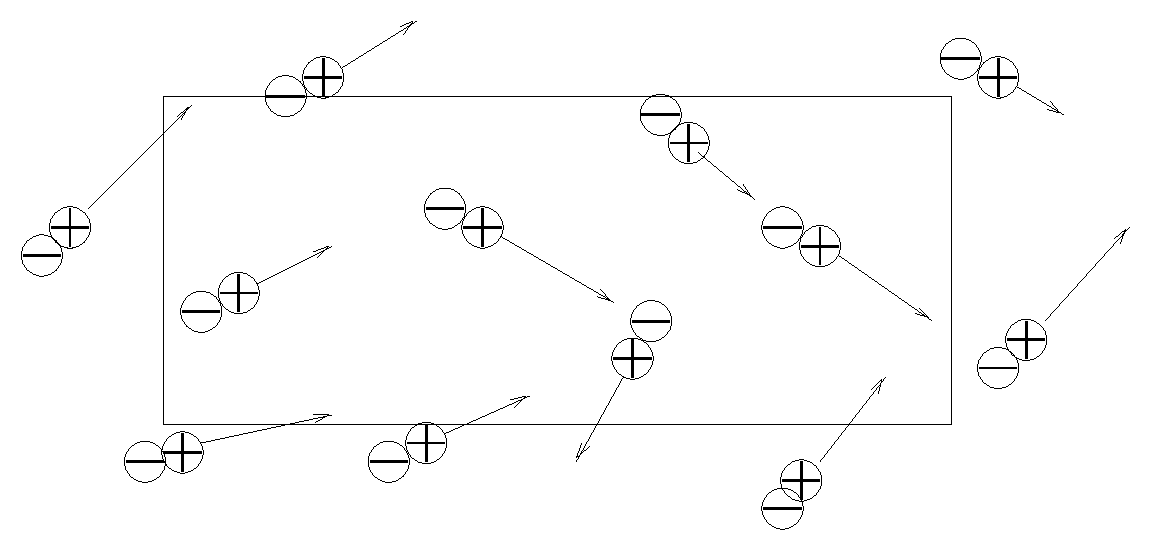
\epsfig{file={../fig/polar}}}   
 \caption{Polarization vector at point $r$ is the limit of the ratio of the
   sum of elementary  dipolar moments contained in the box $d\tau$ over the
   volume $d\tau$ as it tends towards zero.}
 \label{figpolar}
\end{figure}
Maxwell--gauss equation in vacuum
\begin{equation}
\mbox{ div } \epsilon_0E=\rho
\end{equation}
can be written as:
\begin{equation}
\mbox{ div } (\epsilon_0E-P)=0
\end{equation}
We thus have related the microscopic properties of the material (the $p$'s) to
the macroscopic description of the material (by vector $D=\epsilon_0E-P$). We
have now to provide a microscopic model for $p$. Several models can be
proposed. A material can be constituted by small dipoles all oriented in the
same direction. Other materials, like oil, are constituted by molecules
carrying a small dipole, their orientation being random when there is no $E$
field. But when there exist an non zero $E$ field, those molecules tend to
orient their moment along the electric field lines. The mean $P$ of the
$p_i$'s given by equation \ref{eqmoyP} that is zero when $E$ is zero (due to
the random orientation of the moments) becomes non zero in presence of a non
zero $E$. A simple model can be proposed without entering into the details of
a quantum description.
It consist in saying that $P$ is proportional to $E$:
\begin{equation}
P=\chi  E
\end{equation}
where $\chi$ is the polarisability of the medium. In this case relation:
\begin{equation}
D=\epsilon_0E-P
\end{equation}
becomes:
\begin{equation}
D=(\epsilon_0+\chi )E
\end{equation}
\end{exmp}
\begin{exmp}{\bf A second model of susceptibility:}
Consider the Vlasov equation (see equation \ref{eqvlasov} and reference
\cite{ph:physt:Diu89}). Function $f$ is the mean density of particles and
$n_0$ represents the density of the positively charged background.
\begin{equation}\label{vlasdie}
\frac{\partial f}{\partial t}+{v}\partial_x f+\frac{F}{m}\partial_v f= 0
\end{equation}
let us assume that the force undergone by the particles is the electric force:
\begin{equation}
\vec{F}=-eE(x,t)
\end{equation}
Maxwell equations are reduced here to:
\begin{equation}\label{eqmaxsystpart}
\mbox{ div } E=\rho
\end{equation}
where electrical charge $\rho(x,t)$ is the charge induced by the fluctuations
of the electrons around the neutral equilibrium state:
\begin{equation}
\rho=-e\int f(x,v,t)dv+en_0
\end{equation}
Let us linearize this equation system with respect to the following
equilibrium position:
\begin{eqnarray}
f(x,v,t)&=&f^0(v)+f^1(x,v,t)\nonumber\\
F(x,v,t)&=&0+F_1
\end{eqnarray}
As the system is globally electrically neutral:
\begin{equation}
\int f^0(v) = n_0
\end{equation}
By a $x$ and $t$ Fourier transform of equations \ref{vlasdie} and
\ref{eqmaxsystpart} one has:
\begin{eqnarray}
\epsilon_0 ik \hat{E_1}&=&-e\int \hat{f_1} dv\\
-i\omega \hat{f_1}+ivk\hat{f_1}&=&e\frac{\hat{E_1}}{m} \frac{\partial
\hat{f^0}}{\partial v} 
\end{eqnarray}
Eliminating $\hat{f_1}$ from the previous system, we obtain:
\begin{equation}
ik\hat{E_1}(\epsilon_0 - \frac{e^2}{km}\int
\frac{1}{vk-\omega}\frac{\partial \hat f^0}{\partial v}dv)=0
\end{equation}
The first term of the previous equation can be considered as the divergence of
a vector that we note $D$ which is $D=\epsilon*E_1$, where $*$ is the
convolution in $x$ and $t$ :
\begin{equation}\label{eqmaxconvol}
\mbox{ div }(\epsilon *E_1)=0
\end{equation}
Vector $D$ is called electrical displacement. $\epsilon$ is the susceptibility
of the medium. Maxwell equations \ref{eqmaxsystpart} describing a system of
charges in vacuum has thus been transformed to equation \ref{eqmaxconvol} that
described the field in matter. Previous equation provides $\epsilon
(k,\omega)$: 
\begin{equation}
\epsilon (k,\omega)=(\epsilon_0 - \frac{e^2}{km}\int
\frac{1}{vk-\omega}\frac{\partial \hat{f}^0}{\partial v}dv)
\end{equation}
\end{exmp}
\section{Generalized elasticity}\label{secelastigene} 
%%%%%%%%%%%%%%%%%%%%%%%%%%%%
\subsection{Introduction}
%%%%%%%%%%%%%%%%%
In this section, the concept of elastic energy is presented.
\index{elasticity} 
The notion of elastic energy allows to deduce easily ``strains--deformations''
relations.\index{strain--deformation relation} 
So, in modelization of matter by virtual powers method
\index{virtual powers}
a power $P$ that is a functional of displacement is introduced.
Consider in particular case of a mass $m$ attached to a spring of constant
$k$. {\bf Deformation} of the system is referenced by the elongation $x$ of the
spring with respect to equilibrium.
The {\bf virtual work}
\index{virtual work}
associated to a displacement
$dx$ is 
\begin{equation}\label{deltWfdx}
\delta W=f.dx
\end{equation}
Quantity $f$ represents the {\bf constraint}, here a force, and
$x$ is the deformation. If force  $f$ is conservative, then it is known that
the elementary work (provided by the exterior) is the total differential of a
potential energy function or {\bf internal energy} $U$ :
\begin{equation}\label{eqdeltaWdU}
\delta W=-dU
\end{equation}
In general, force $f$ depends on the deformation. Relation $f=f(x)$ is thus a
{\bf constraint--deformation relation}.


The most natural way to find the strain-deformation relation is the
following. One looks for the expression of $U$ as a function of the
deformations using the physics of the the problem and symmetries. In the
particular case of an oscillator, the internal energy has to depend only on
the distance  $x$ to equilibrium position. If $U$ admits an expansion at
$x=0$, in the neighbourhood of the equilibrium position $U$ can be approximated
by:
\begin{equation}
U(x)=a_0+a_1x^1+a_2x^2+O(x^2)
\end{equation}
As $x=0$ is an equilibrium position, we have $dU=0$ at $x=0$. That implies that
$a_1$ is zero. Curve $U(x)$ at the neighbourhood of equilibrium has thus a
parabolic shape (see figure \ref{figparabe}
\begin{figure}[htb]
 \centerline{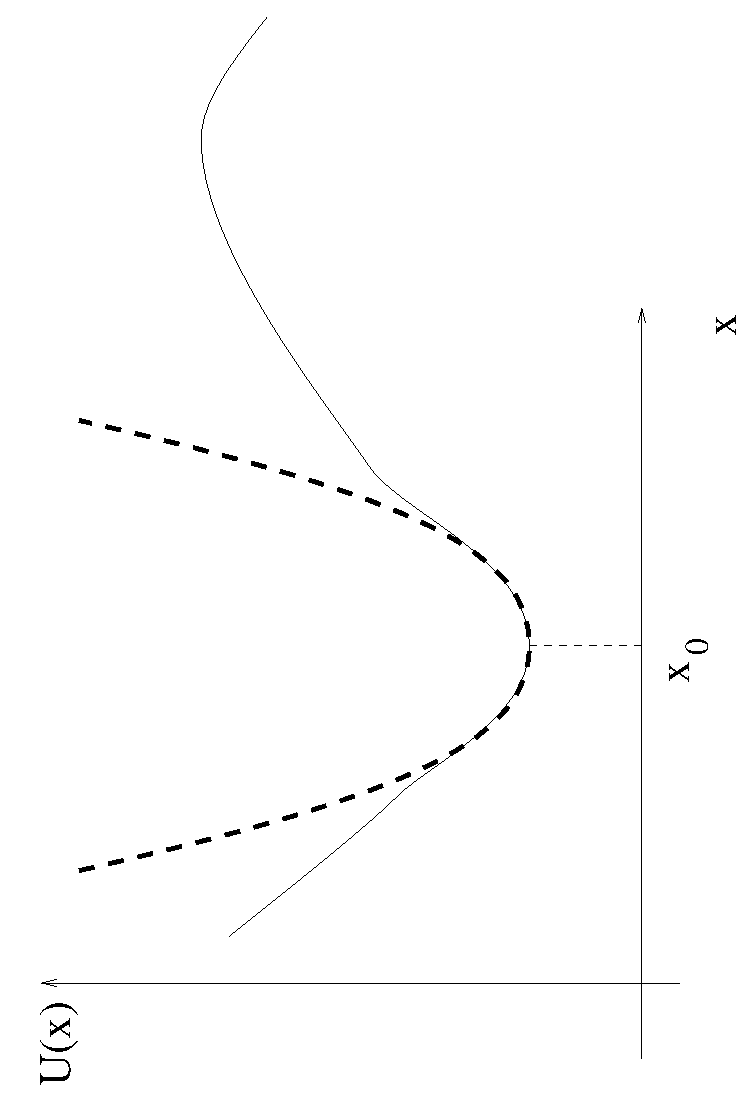
\epsfig{file={../fig/parabe}}}   
 \caption{In the neighbourhood of a stable equilibrium position $x_0$, the
   intern energy function $U$, as a function of the difference to equilibrium
   presents a parabolic profile.}
 \label{figparabe}
\end{figure}
As
\begin{equation}
dU=-fdx
\end{equation}
the strain--deformation relation becomes:
\begin{equation}
f=\frac{dU}{dx}
\end{equation}
\subsection{Oscillators chains}
%%%%%%%%%%%%
Consider a unidimensional chain of $N$ oscillators coupled by springs of
constant $k_{ij}$. this system is represented at figure
\ref{figchaineosc}. Each oscillator is referenced by its difference position
$x_i$ with respect to equilibrium position.
A calculation using the Newton's law of motion implies:
\begin{equation}
U=\sum\frac{1}{2}k_{ij}(x_i-x_{j-1})^2
\end{equation}
\begin{figure}[htb]
 \centerline{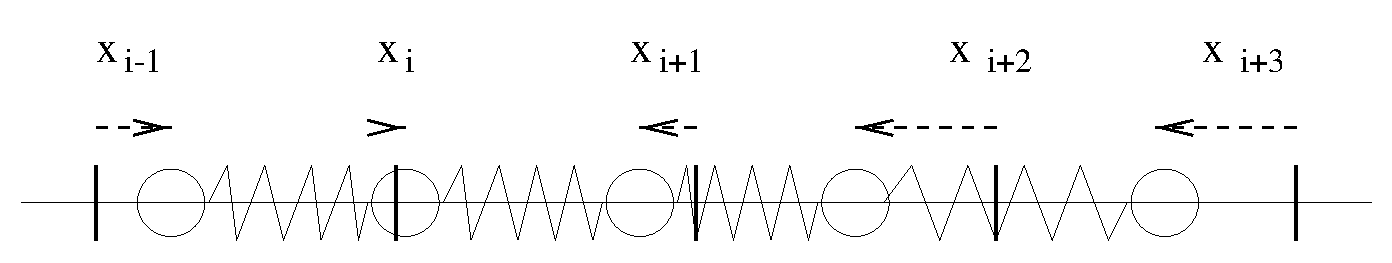
\epsfig{file={../fig/chaineosc}}}   
 \caption{A coupled oscillator chain is a toy example for studying
   elasticity.} 
 \label{figchaineosc}
\end{figure}
A calculation using virtual powers principle would have consisted in
affirming:
The total elastic potential energy is in general a function $U(x_1,\dots,
x_N)$ of the differences $x_i$ to the equilibrium positions. This differential
is total since force is conservative\footnote{%%%%%%%
This assumption is the most difficult to prove in the theories on elasticity
as it will be shown at next section}%%%%%%%%
. So, at equilibrium:
\index{equilibrium} :
\begin{equation}
dU=0
\end{equation}
If $U$ admits a Taylor expansion:
\begin{equation}\label{eqdevliUch}
U(x_1=0,\dots x_N=0)=a+a_i x_i+a_{ij}x_ix_j+O(x^2)
\end{equation}
In this last equation, repeated index summing convention as been used. Defining
the differential of the intern energy as:
\begin{equation}
dU=f_i dx_i
\end{equation}
one obtains
\begin{equation}
f_i=\frac{\partial U}{\partial x_i}.
\end{equation}
Using expression of $U$ provided by equation \ref{eqdevliUch} yields to:
\begin{equation}
f_i=a_{ij}x_j.
\end{equation}
But here, as the interaction occurs only between nearest neighbours, variables
$x_i$ are not the right thermodynamical variables.
let us choose as thermodynamical variables the variables $\epsilon_i$ defined
by: 
\begin{equation}
\epsilon_i=x_i-x_{i-1}.
\end{equation}
Differential of $U$ becomes:
\begin{equation}
dU=F_id\epsilon_i
\end{equation}
Assuming that $U$ admits a Taylor expansion around the equilibrium position:
\begin{equation}
U=b+b_i\epsilon_i+b_{ij}\epsilon_i\epsilon_j+O(\epsilon^2)
\end{equation}
and that $dU=0$ at equilibrium, yields to:
\begin{equation}
F_i=b_{ij}\epsilon_j
\end{equation}
As the interaction occurs only between nearest neighbours:
\begin{equation}
b_{ij}=0 \mbox{ si  } i\neq j\pm 1
\end{equation}
so:
\begin{equation}
F_i=b_{ii}\epsilon_i+b_{ii+1}\epsilon_{i+1}
\end{equation}
This does correspond to the expression of the force applied to mass $i$ :
\begin{equation}
F_i=-k(x_{i}-x_{i-1})-k(x_{i+1}-x_{i})
\end{equation}
if one sets $k=-b_{ii}=-b_{ii+1}$.
\subsection{Tridimensional elastic material}\label{secmaterelast}
%%%%%%%%%%%
Consider a system $S$ in a state $S_X$ which is a deformation from the state
$S_0$. Each particle position is referenced by a vector $a$ in the state
$S_0$ and by the vector $x$ in the state $S_X$:
\begin{equation}
x=a+X
\end{equation}
Vector $X$ represents the deformation.
\begin{rem}
Such a model allows to describe for instance fluids and solids.
\end{rem}
Consider the case where $X$ is always ``small''. Such an hypothesis is called
small perturbations hypothesis (SPH). The intern energy is looked as a function
 $U(X)$. 
\begin{defn}
The deformation tensor SPH is the symmetric part of the tensor gradient of $X$.
\begin{equation}
\epsilon_{ij}=\frac{1}{2}(X_{i,j}-X_{j,i})
\end{equation}
\end{defn}
At section \ref{secpuisvirtu} it has been seen that the power of the
admissible intern strains for the problem considered here is:
\begin{equation}
P_i=\int K_{ij}^s u_{i,j}^s d\tau
\end{equation}
with
\begin{equation}
dU=-P_idt
\end{equation}
Tensor $u_{i,j}^s$ is called rate of deformation tensor. It is the symmetric
part of tensor $u_{i,j}$. It can be shown \cite{ph:fluid:Germain80} that in
the frame of SPH hypothesis, the rate of deformation tensor is simply the time
derivative of SPH deformation tensor:
\begin{equation}
u_{i,j}^s=\frac{d\epsilon_{ij}}{dt}
\end{equation}
Thus:
\begin{equation}\label{dukij}
dU=-\int K_{ij}^s d\epsilon_{ij}d\tau.
\end{equation}
Function $U$ can thus be considered as a function $U(\epsilon_{ij})$. More
precisely, one looks for $U$ that can be written:
\begin{equation}
U=\int \rho e_l d\tau
\end{equation}
where $e_l$ is an internal energy density with\footnote{%%%
Function $U$ depends only on $\epsilon_{ij}$.} %%%%%%%%%%%%%%%%%%%%%%%
whose Taylor expansion around the equilibrium position is:
\begin{equation}\label{eqrhoel}
\rho e_l=a+a_{ij}\epsilon_{ij}+a_{ijkl}\epsilon_{ij}\epsilon_{kl}
\end{equation}
We have\footnote{\label{footdensi}Indeed:%%%%%%%%%% 
\begin{equation}
\frac{d}{dt}U=\frac{d}{dt}\int \rho e_l d\tau
\end{equation}
and from the properties of the particulaire derivative:
\begin{equation}
\frac{d}{dt}\int \rho e_l d\tau=\int\frac{d}{dt}( \rho e_l d\tau)
\end{equation}
Now,
\begin{equation}
\frac{d}{dt} (\rho e_ld\tau)=e_l\frac{d}{dt} (\rho d\tau) + \rho
d\tau\frac{d}{dt}e_l 
\end{equation}
From the mass conservation law:
\begin{equation}
\frac{d}{dt} \rho=0
\end{equation}
}%%%%%%%%%%%%%%%%%%%%%%%%%%%%
\begin{equation}\label{eqdudt}
\frac{dU}{dt}=\int \rho (\frac{d}{dt}e_l) d\tau
\end{equation}
Thus
\begin{equation}
dU=\int \rho de_l d\tau
\end{equation}
Using expression \ref{eqrhoel} of $e_l$ and assuming that $dU$ is zero at
equilibrium, we have:
\begin{equation}
dU=\int \rho  [a_{ijkl}\epsilon_{ij}d\epsilon_{kl}+
a_{ijkl}d\epsilon_{ij}\epsilon_{kl}]d\tau 
\end{equation}
thus:
\begin{equation}
dU=\int \rho  b_{ijkl}\epsilon_{kl}d\epsilon_{ij}d\tau
\end{equation}
with $b_{ijkl}=a_{ijkl}+a_{klij}$. Identification with equation
\ref{dukij},  yields to the following strain--deformation relation:
\begin{equation}
K_{ij}^s=b_{ijkl}\epsilon_{kl}
\end{equation}
it is a generalized Hooke law\index{Hooke law}. The $b_{ijkl}$'s are the
elasticity coefficients. 
\begin{rem}
Calculation of the footnote \ref{footdensi} show that calculations done at
previous section \ref{secchampdslamat} should deal with volumic energy
densities. 
\end{rem}

\subsection{Nematic material}\label{secenernema}
%%%%%%%%%%%
A nematic material\index{nematic} is a material
\cite{ph:liqcr:DeGennes74} whose state can be defined by vector
field\footnote{%%%%%%%%%%%%%%%%%%%
State of smectic materials can be defined by a function
$u(x,y)$.%%%%%%%%%%%%%%%%%
}  $n$. This field is related to the orientation of the molecules in the
material (see figure
\ref{figchampnema})
\begin{figure}[htb]
 \centerline{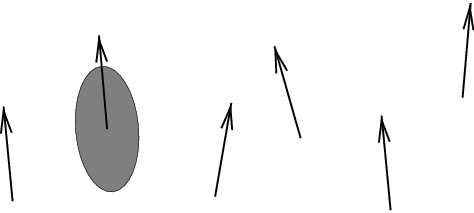
\epsfig{file={../fig/champnema}}}   
 \caption{Each molecule orientation in the nematic material can be described
   by a vector $n$. In a continuous model, this yields to a vector field
   $n$. Internal energy of the nematic is a function of the vector field $n$
   and its partial derivatives.}
 \label{figchampnema}
\end{figure}
Let us look for an internal energy $U$ that depends on the gradients of the $n$
field:
\begin{equation}
U=\int u d\tau
\end{equation}
with
\begin{equation}
u=u_1(\partial_in_j)+u_2(n_i\partial_jn_k)+ u_3(\partial_i
n_j\partial_kn_l)+ u_4(n_pn_q\partial_i n_j\partial_kn_l)+\dots
\end{equation}
The most general form of $u_1$ for a linear dependence on the derivatives is:
\begin{equation}\label{eqsansder}
u_1(\partial_in_j)= K_{ij} \partial_i n_j
\end{equation}
where $K_{ij}$ is a second order tensor depending on $r$.
Let us consider how symmetries can simplify this last form.
\begin{itemize}
\item {\bf Rotation invariance.}
Functional $u_1$ should be rotation invariant.
\begin{equation}
u_1(\partial_i n_j)=u_1(R_{ik}R_{jl}\partial_k n_l)
\end{equation}
where $R_{mn}$ are orthogonal transformations (rotations). We thus have the
condition: 
\begin{equation}
K_{ij}=R_{ik}R_{jl}K_{kl},
\end{equation}
that is, tensor $K_{ij}$ has to be isotrope. It is know that the only second
order isotrope tensor in a three dimensional space is $\delta_{ij}$, that is
the identity. So $u_1$ could always be written like:
\begin{equation}
u_1=k_0\mbox{ div } n
\end{equation}
\item {\bf Invariance under the transformation $n$ maps to $-n$}. The energy
  of distortion is independent on the sense of $n$, that is
  $u_1(n)=u_1(-n)$. This implies that the constant $k_0$ in the previous
  equation is zero. 
\end{itemize}
Thus, there is no possible energy that has the form given by equation
\ref{eqsansder}. This yields to consider next possible term $u_2$. general
form for $u_2$ is:
\begin{equation}
u_2=L_{ijk}n_k\partial_in_j
\end{equation}
Let us consider how symmetries can simplify this last form.
\begin{itemize}
\item {\bf Invariance under the transformation $n$ maps to $-n$}. This
  invariance condition is well fulfilled by $u_2$.
\item {\bf Rotation invariance.} The rotation invariance condition implies
  that:
\begin{equation}
L_{ijk}=R_{il}R_{jm}R_{kn}L_{lmn}
\end{equation}
It is known that there does not exist any third order isotrope tensor in
$R^3$, but there exist a third order isotrope pseudo tensor: the signature
pseudo tensor $e_{jkl}$ (see appendix \ref{secformultens}). This yields to the
expression: 
\begin{equation}
u_2=k_1e_{ijk}n_k\partial_in_j=k_1n\mbox{ rot } n.
\end{equation}
\item {\bf Invariance of the energy with respect to the axis transformation
    $x\rightarrow -x$, $y\rightarrow -y$, $z\rightarrow -z$.} The energy of
  nematic crystals has this invariance property\footnote{%%%%%%%%%%
Cholesteric crystal doesn't verify this condition.}%%%%%%
. Since $e_{ijk}$ is a pseudo-tensor it changes its signs for such
transformation.
\end{itemize}
There are thus no term $u_2$ in the expression of the internal energy for a
nematic crystal.
Using similar argumentation, it can be shown that $u_3$ can always be
written:
\begin{equation}
u_3=K_1 (\mbox{ div } n)^2
\end{equation}
and $u_4$:
\begin{equation}
u_4=K_2 (n.\mbox{ rot } n)^2+K_3(n \wedge \mbox{ rot } n)^2
\end{equation}
Limiting the development of the density energy $u$ to second order partial
derivatives of $n$ yields thus to the expression:
\begin{equation}
u=K_1 (\mbox{ div } n)^2+K_2 (n.\mbox{ rot } n)^2+K_3(n \wedge \mbox{ rot } n)^2
\end{equation}


\section{Other phenomena}
%%%%%%%%%%%%%%%%%%%%%%%
\subsection{Piezoelectricity }\label{secpiezo}
%%%%%%%%%%%%%%%%%
In the study of {\bf piezoelectricity}
\cite{ph:elect:LandauEle}, on\index{piezo electricity} 
the form chosen for $\sigma_{ij}$ is:
\begin{equation}
\sigma_{ij}=\lambda_{ijkl}u_{kl}+\gamma_{ijk}E_k
\end{equation}
The tensor $\gamma_{ijk}$ traduces a coupling between electrical field
variables $E_i$ and the deformation variables present in the expression of
$F$: 
\begin{equation}
F=F_0+\epsilon_{ij}E_iE_j+\frac{1}{2}\lambda_{ijkl}u_{ij}u_{kl}+
\gamma_{ijk}E_iu_{jk}. 
\end{equation}
The expression of $D_i$ becomes:
\begin{equation}
D_i=\left.\frac{\partial F}{\partial E_i}\right)_{u_{fixed},T_{fixed}}
\end{equation}
so:
\begin{equation}
D_i=\epsilon_{ij}E_j+\gamma_{ijk}u_{jk}
\end{equation}

\subsection{Viscosity}
%%%%%%%%%%%%%%%%%%%
A material is called viscous
\index{viscosity}
each time the strains depend
on the deformation speed. In the {\bf linear viscoelasticity}
theory\cite{ma:equad:Dautray1}, the following
strain-deformation relation is adopted:
\begin{equation}
\sigma_{ij}=a_{ijkl}u_{kl}+b_{ijkl}\frac{\partial u_{kl}}{\partial t}
\end{equation}
Material that obey such a law are called {\bf short memory
  materials}
\index{memory}
since the state of the constraints at time $t$
depends only on the deformation at this time and at times infinitely close to
$t$ (as suggested by a Taylor development of the time derivative). Tensors $a$
and $b$ play respectively the role of elasticity and viscosity coefficients.
If the strain-deformation relation is chosen to be:
\begin{equation}\label{eqmatmem}
\sigma_{ij}=a_{ijkl}u_{kl}+\int_0^tb_{ijkl}(t-s)u_{kl}(s)ds,
\end{equation}
then the material is called {\bf long memory} material since the state of the
constraints at time $t$ depends on the deformation at time $t$ but also on
deformations at times previous to $t$.
The first term represents an instantaneous elastic effect. The second term
renders an account of the memory effects.
\begin{rem}
Those materials belong \cite{ma:equad:Duvaut72} to a special class of
materials called {\it rate type} for which there exist a linear relation
between time derivatives of tensors deformation and strain tensors:
\begin{equation}
\sigma_{ij}(t)+a^1_{ijkl}\frac{\partial \sigma_{kl}(t)}{\partial
t}+\dots+a^{n_1}_{ijkl}\frac{\partial^{n_1} \sigma_{kl}(t)}{\partial
t^{n_1}} 
\end{equation}
\begin{equation}
=b^0_{ijkl}u_{kl}(t)+b^1_{ijkl}\frac{\partial u_{kl}(t)}{\partial
t}+\dots+b^{n_2}_{ijkl}\frac{\partial^{n_2} u_{kl}(t)}{\partial
t^{n_2}} 
\end{equation}
By Laplace transform, it can be shown that it is equivalent to consider a law:
\begin{equation}
\sigma_{ij}(t)=A^0_{ijkl}u_{kl}(t)+A^1_{ijkl}\frac{\partial
u_{kl}(t)}{\partial t}+\dots+A^{N}_{ijkl}\frac{\partial^{N}
u_{kl}(t)}{\partial t^{N}}+b_{ijkl}*u_{kl}(t) 
\end{equation}
where $N=n_2-n_1$ and where $b(t)$ is a regular function.
\end{rem}
\begin{rem}
In the frame of distribution theory, time derivatives can be considered as
convolutions by derivatives of Dirac distribution. For instance, time
derivation can be expressed by the convolution by $\delta '(t)$. This allows
to treat this case as a particular case of formula given by
equation\ref{eqmatmem}. 
\end{rem}

\section{Exercises}
%%%%%%%%%%%%%%%%%

\begin{exo}
Find the equation evolution for a rope clamped between two walls.
\end{exo}

\begin{exo}
Find the equation describing the sound propagation in a air column. To obtain
the dynamics equation, methods seen at previous chapter will be used
(conservation laws of virtual powers principle). To obtain the
strain--deformation relation, it will be assumed that the gas undergoes
adiabatic transformations, {\it i.e.}
$pV^{\gamma}$=constant, where $p$ is the gas pressure, $V$ the air volume and
$\gamma$ a constant.
\end{exo}

\begin{exo}
Give the expression of the deformation energy of a smectic (see section
\ref{secristliquides} for the description of smectic) whose
i$^th$ layer's state is described by surface $u_i(x,y)$,
\end{exo}

\begin{exo}
Consider a linear, homogeneous, isotrope material. Electric susceptibility
$\epsilon$ introduced at section \ref{secchampdslamat} allows for such
materials to provide $D$ from $E$ by simple convolution:
\begin{equation}\label{eqexsusc}
D=\epsilon * E.
\end{equation}
where $*$ represents a temporal convolution. To obey to the causality
principle distribution $\epsilon$ has to have a positive support. Indeed, $D$
can not depend on the future values of $E$. Knowing that the Fourier
transform of function ``sign of $t$'' is $C.V_p(1/x)$ where $C$ is a
normalization constant and $V_p(1/X)$ is the principal value of $1/x$
distribution, give the relations between the real part and imaginary part of
the Fourier transform of $\epsilon$.  These relations are know in optics as
{\bf Krammers--Kr\"onig} relations\index{Krammers--Kr\"onig relations}.
\end{exo}

\appendix
%%%%%%%%%%%%%%%%%%%




\chapter{Measure and integration}
%%%%%%%%%%%%%%%%%%%%%%%%%%%%%%%%%

\section{Lebesgue integral}
%%%%%%%%%%%%%%%%%%%%%%%%%%%
The theory of the Lebesgue integral is difficult and can not be
presented here. However, we propose here to give to the reader an idea of the
Lebesgue integral based on its properties. 
The integration in the Lebesgue sense is a fonctional that at each
element $F$ of a certain functional space (the space of the summable
functions) associates a number note $\int f(x) dx$ of $\int f$.
\begin{enumerate}
\item for a function $f$ to be summable, it is sufficient that $|f|$
is summable.
\item if $g(x)\geq 0$ is summable  and if $|f(x)|\leq g(x)$ then
$f(x)$ is summable and
\begin{equation}
|\int f\leq\int|f|\leq\int g
\end{equation}
\item If $f$ and $g$ are almost everywhere equal, the their sum is
egual.
\item if $f(x)\geq 0$ and if $\int f=0$ then $f$ is almost everywhere
zero.
\item A bounded function, zero out of a finite interval $(a,b)$ is
summable. If $f$ is integrable in the Riemann sense on $(a,b)$ then
the sums in the Lebesgue and Rieman sense are egual.
\end{enumerate}



%%%%%%%%%%%%%%%%%%%%%%%%%%%%%%%%%%%%%%%%%%%%%%
\chapter{Groups}\label{chapgroupes}
%%%%%%%%%%%%%%%%%
\section{Definition}
%%%%%%%%%%%%%%%%%%%%%%%%%%%%%%%%%%%%%%%%%%%%%
In classical mechanics,\index{group} translation and rotation invariances
correspond to momentum and kinetic moment conservation. Noether theorem allows
to bind symmetries of Lagrangian and conservation laws.
The underlying mathematical theory to the intuitive notion of symmetry is
presented in this appendix.
\begin{defn}
A {\bf group} is a set of elements $G=\{g_1,g_2,\dots\}$ and a composition law
$.$ that assigns to any ordered pair $(g_1,g_2)\in G$ an element $g_1.g_2$ of
$G$. The composition law $.$ is 
\begin{itemize}
\item associative
\begin{equation}
g_1.(g_2.g_3)=(g_1.g_2).g_3
\end{equation}
\item has a unit element $e$ :
\begin{equation}
g.e=e.g=e
\end{equation}
\item for each $g$ of $G$, there exists an element $g^{-1}$ of
$G$ such that:
\begin{equation}
g.g^{-1}=g^{-1}.g=e
\end{equation}
\end{itemize}
\end{defn}
\begin{defn}
The order of a group is the number of elements of $G$.
\end{defn}

\section{Representation}
%%%%%%%%%%%%%%%%%%%%%%%
For a deeper study of group representation theory, the reader is invited to
refer to the abundant litterature (see for instance 
\cite{ph:mecaq:Pauling60,ma:group:Jones90,ma:group:Kettle95}).
\begin{defn}
A {\bf representation} of a group $G$ in a vectorial space $V$ on $K=R$ or
$K=C$ is an endomorphism $\Pi$ from $G$ into the group
$GL(V)$\footnote{$GL(V)$ is the space of the linear applications from $V$
into $V$. It is a group with respect to the function composition
law.}%%%%%% 
{\it i.e }a
mapping 
\begin{equation}
\begin{array}{llll}
\Pi:&G&\longrightarrow &GL(V)\\
  &g&\longrightarrow &\Pi(g)
\end{array}
\end{equation}
with
\begin{equation}
\Pi(g_1.g_2)=\Pi(g_1).\Pi(g_2)
\end{equation}
\end{defn}
\begin{defn}
Let $(V,\Pi)$ be a representation of $G$. A vectorial subspace 
$W$ of $V$ is called stable by $\Pi$ if:
\begin{equation}
\forall g\in G, \Pi(g).W\subset V. 
\end{equation}
One then obtains a representation of $G$ in $W$ called subrepresentation of
$\Pi$.
\end{defn}
\begin{defn}
A representation $(V,\Pi)$ of a group $G$ is called {\bf irreducible} if it
admits no subrepresentation other than $0$ and itself.
\end{defn}
Consider a symmetry group $G$. let us consider some classical examples of
vectorial spaces $V$.
Let ${\cal{R}}$ be an element of $G$.
\begin{exmp}\label{exampgroupR}
Let $G$ be a group of transformations ${\cal r}$ of space $R^3$. A
representation $\Pi_1$ of $G$ in $V=R^3$ is simply defined by:
\begin{equation}
\begin{array}{llll}
\Pi_1({\cal{r}}):&R^3&\longrightarrow &R^3\\
  &\vec{x}&\longrightarrow &\vec{x}'={\cal{R}}(\vec{x})
\end{array}
\end{equation}
To each element ${\cal r}$ of $G$, a mapping ${\cal{R}}$ of $R^3$ is
associated. This mapping can be defined by a matrix $M$ called representation
matrix of symmetry operator ${\cal r}$.
\end{exmp}
\begin{exmp}
Let us consider molecule $NH_3$ as a solid of symmetry $C_3$. The various
symmetry operations that characterizes this group are:
\begin{itemize}
\item three reflexions $\sigma_1$,$\sigma_2$, and $\sigma_3$.
\item two rotations around the $C_3$ axis, of angle 
$\frac{2\pi}{3}$ and $\frac{4\pi}{3}$ noted $C_3^1$ and $C_3^2$.
\item rotation of angle  $\frac{6\pi}{3}$ is the identity and is noted $E$.
\end{itemize}
In a any basis of $R^3$, representation matrices of group symmetry operators
are in general not block diagonal.

The tridimensional space can be shared into two invariant subspaces: a
one-dimensional space $E_1$ spanned by vector of the $C_3$ axis, and a plane
$E_3$ perpendicular to this vector.
In chemistry books, representation on $E_1$ is called $A$ and representation
on $E_2$ is called $E$. They are both irreducible.
\end{exmp}
\begin{rem}
For the study of the vibrations of a molecule, instead of considering the
Euclidian space $R^3$ as state space, the space of the $q_i$'s where the
$q_i$'s are the degree of freedom of the system has to be considered. The
diagonalization of the coupling matrix problem can be tackled using symmetry
considerations. Indeed, a vibratory system is invariant by symmetry $G$,
implies that its energy is invariant by $G$:
\begin{equation}
\forall g\in G, \forall x\in V, <M^+(g)x|KM(g)x>=<x|Kx>
\end{equation}
Matrices $M(g)$ being orthonormal, kinetic energy is also invariant.
\end{rem}
Consider the following theorem:
\begin{thm}\label{theosymde}
If operator $A$ is invariant by $R$, that is
$\rho_RA=A$ or $RAR^{-1}=A$, the if $\phi$ is eigenvector of $A$,  $R\phi$ is
also eigenvector of $A$.
\end{thm}
\begin{pf}
It is sufficient to evaluate the action of $A$ on $R\phi$ to prove this
theorem. 
\end{pf}
This previous theorem allows to predict the eigenvectors and their degeneracy.
\begin{exmp}
Consider the group $G$ introduced at example \ref{exampgroupR}. A
representation $\Pi_2$ of $G$ in the space $L^2$ of summable squared
can be defined by:
\begin{equation}
\begin{array}{llll}
\Pi_2({\cal{r}}):&L^2(R^3)&\longrightarrow &L^2(R^3)\\
  &f(x)&\longrightarrow &Rf(x)=f({\cal{R}}^{-1}(\vec{x}))
\end{array}
\end{equation}
where ${\cal R}=\Pi_1({\cal r})$ is the matrix representation of
transformation ${\cal r}$, element of $G$.
If $\phi_i$ is a basis of $L^2(R^3)$, then we have $R\phi_i=D_{ki}\phi_i$.
\end{exmp}
\begin{exmp}
Consider the group $G$ introduced at example \ref{exampgroupR}. A
representation $\Pi_3$ of $G$ in the space of linear operators of
$L^2$ can be defined by:
\begin{equation}
\begin{array}{llll}
\Pi_3({\cal{r}}):&{\cal{L}}(L^2(R^3))&\longrightarrow &{\cal{L}}(L^2(R^3))\\
  &A&\longrightarrow &\rho_A=RAR^{-1}
\end{array}
\end{equation}
where $R=\Pi_2({\cal r})$ is the matrix representation, defined at
prevoius example, of
transformation ${\cal r}$, element of $G$ and $A$ is the matrix
defining the operator
\end{exmp}

Relatively to the $R^3$ rotation group, scalar, vectorial and tensorial
operators can be defined.
\begin{defn}
A {\bf scalar} operator $S$ is invariant by rotation:
\begin{equation}
RSR^{-1}=S
\end{equation}
\end{defn}
An example of scalar operator is the hamiltonian operator in quantum
mechanics.
\begin{defn}
A vectorial operator $V$ is a set of three operators $V_m$, 
$m=-1,0,1$, (the components of $V$ in spherical coordinates) that verify the
commutation relations:
\begin{equation}
[X_i,V_m]=\epsilon_{imk}V_k
\end{equation}
\end{defn}
More generally, tensorial operators can be defined:
\begin{defn}
A tensorial operator $T$ of components $T_m^j$ is an operator whose
transformation by rotation is given by:
\begin{equation}
RT_m^jR^{-1}=D_{m'm}^j(R)T_{m'}^j
\end{equation}
where $D_{m'm}^j(R)$ is the restriction of rotation $R$ to space spanned by
vectors $|jm>$.
\begin{equation}
D_{m'm}^j(R)=<jm'|R|jm>
\end{equation}
\end{defn}
Another equivalent definition is presented in \cite{ph:mecaq:Cohen73}. It can
be shown that a vectorial operator is a tensorial operator with $j=1$.
This interest of the group theory for the physicist is that it provides
irreducible representations of symmetry group encountered in Nature. Their
number is limited. It can be shown for instance that there are only 32 symmetry
point groups allowed in crystallography. There exists also methods to expand
into irreducible representations a reducible representation (see
\cite{ma:group:Kettle95}). 

\section{Tensors and symmetries}
%%%%%%%%%%%%%%%%%%%%
Let $a_{ijk}$ be a third order tensor. Consider the tensor:
\begin{equation}
X_{ijk}=x_ix_jx_k
\end{equation}
let us form the density: 
\begin{equation}
\phi=a_{ijk}X_{ijk}
\end{equation}
$\phi$ is conserved by change of basis\footnote{%
A unitary operator preserves the scalar product.}
If by symmetry:
\begin{equation}
Ra_{ijk}=a_{ijk}
\end{equation}
then
\begin{equation}
RX_{ijk}=X_{ijk}
\end{equation}
With other words ``X is transformed like
$a$''\cite{ma:tense:Bass64,ma:tense:Brillouin64}  
\begin{exmp} : {\bf piezoelectricity.}
As seen at section \ref{secpiezo}, there exists for piezoelectric materials a
relation between the deformation tensor $e_{ij}$ and the electric field $h_k$
\begin{equation}
e_{ij}=a_{ijk}h_k
\end{equation}
$a_{ijk}$ is called the piezoelectric tensor. Let us show how previous
considerations allow to obtain following result:
\begin{thm}
If a crystal has a centre of symmetry, then it can not be piezoelectric.
\end{thm}
\begin{pf}
Let us consider the operation $R$ symmetry with respect to the centre, then
\begin{equation}
R(x_ix_jx_k)=(-1)^3x_ix_jx_k.
\end{equation}
The symmetry implies
\begin{equation}
Ra_{ijk}=a_{ijk}
\end{equation}
so that
\begin{equation}
a_{ijk}=-a_{ijk}
\end{equation}
which prooves the theorem.
\end{pf}
\end{exmp}




\chapter{Vectorial spaces}
%%%%%%%%%%%%%%%%%%%%%%%%%%%
\section{Definition}
%%%%%%%%%%%%%%%%%%%%
Let $K$ be $R$ of $C$. An ensemble $E$ is a vectorial space if it has
an algebric structure defined by to laws $+$ and $.$, such that every
linear combination of two elements of $E$ is inside $E$.
More precisely:

\begin{defn}
An ensemble $E$ is a vectorial space if it has
an algebric structure defined by to laws, a composition law noted  $+$
and an action law noted $.$, those laws verifying:
\begin{enumerate}
\item $(E,+)$ is a commutative group.
\item 
$\forall (\alpha,\beta)\in K\times K, \forall x\in E 
\alpha(\beta x)=(\alpha\beta) x$
\item $\forall x\in E ,1.x=x$ where $1$ is the unity of $.$ law.

\item $\forall (\alpha,\beta)\in K\times K, \forall (x,y)\in E\times E 
(\alpha+\beta) x=\alpha x+\beta x \mbox{ and } \alpha(x+y)=\alpha x+\alpha y
$
\end{enumerate}
\end{defn}


\section{Functional space}
%%%%%%%%%%%%%%%%%%%%%%%%%%
\begin{defn}
A {\bf functional space} is a set ${\cal F}$ of functions that have a
vectorial space 
structure.
\end{defn}
The set of the function continuous on an interval is a functional
space. The set of the positive functions is not a fucntional space.
\begin{defn}
A {\bf functional}  $T$ of ${\cal F}$ is a mapping from ${\cal F}$ into $C$.
\end{defn}
 $<T|\phi>$ designs the number associated to function $\phi$ by functional
 $T$. 
\begin{defn}
A functional $T$ is linear if for any functions $\phi_1$ and
$\phi_2$ of ${\cal F}$ and any complex numbers $\lambda_1$ and
$\lambda_2$ :
\begin{equation}
<T|\lambda_1\phi_1+\lambda_2\phi_2> =
\lambda_1<T|\phi_1>+\lambda_2<T|\phi_2> 
\end{equation}
\end{defn}

\begin{defn}
Space ${\cal D}$ is the vectorial space of functions indefinitely derivable
with a bounded support.
\end{defn}


\chapter{Dual of a vectorial space}
%%%%%%%%%%%%%%%%%%%%%%%%%%%%%%%%%%%%

\section{Dual of a vectorial space}
%%%%%%%%%%%%%%%%%%%%%%%%%%%%%%%%%%%
\subsection{Definition}
%%%%%%%%%%%%%%%%%%%%%%
\begin{defn}
Let $E$ be a vectorial space on a commutative field $K$. The vectorial
space ${\cal L}(E,K)$of
the linear forms on $E$ is called the dual of $E$ and is noted $E^*$.
\end{defn}

When $E$ has  a finite dimension, then $E^*$ has also a finite
dimension and its dimension is gela to the dimension of $E$.
If $E$ has an inifinite dimension, $^*$ has also an inifinite
dimension but the two spaces are not isomorphic.



\subsection{Tensors}\label{chaptens}
%%%%%%%%%%%%%%%%%%
In this appendix, we introduce the fundamental notion of
tensor\index{tensor} in 
physics. More information can be found in \cite{ma:tense:Brillouin64}
for instance. 
Let $E$ be a finite dimension vectorial space.
Let $e_i$ be a basis of $E$.
A vector $X$ of $E$ can be referenced by its components $x^i$ is the basis
$e_i$: 
\begin{equation}
X=x^ie_i
\end{equation}
In this chapter the {\bf repeated index convention} (or {\bf Einstein summing
  convention}) 
will be used. It consists in considering that a product of two quantities with
the same index correspond to a sum over this index. For instance:
\begin{equation}
x^ie_i=\sum_i x^ie_i
\end{equation}
or
\begin{equation}
a_{ijk}b_{ikm}=\sum_i\sum_k a_{ijk}b_{ikm}
\end{equation}
To the vectorial space $E$ correspond a space $E^*$ called the dual of $E$. A
element of $E^*$ is a {\bf linear form} on $E$: it is a linear mapping $p$
that maps any vector $Y$ of $E$ to a real. $p$ is defined by a set of number
$x_i$ because the most general form of a linear form on $E$ is:
\begin{equation}
p(Y)=x_iy^i
\end{equation}
A basis $e^i$ of $E^*$ can be defined by the following linear form
\begin{equation}
e^je_i=\delta_i^j
\end{equation}
where $\delta_i^j$ is one if $i=j$ and zero if not.
Thus to each vector $X$ of $E$ of components $x^i$ can be associated a dual
vector in $E^*$ of components $x_i$:
\begin{equation}
X=x_ie^i
\end{equation}
The quantity
\begin{equation}
|X|=x_ix^i
\end{equation}
is an invariant. It is independent on the basis chosen.
On another hand, the expression of the components of vector $X$ depend on the
basis chosen. If $\omega_k^i$ defines a transformation that maps basis $e_i$
to another basis $e'_i$ 
\begin{equation}\label{eqcov}
e'_i=\omega^k_ie_k
\end{equation}
we have the following relation between components $x_i$
of $X$ in $e_i$ and $x'_i$ of $X$ in $e'_i$:
\begin{equation}\label{eqcontra}
x^i=\omega^i_kx'^k
\end{equation}
This comes from the identification of
\begin{equation}
X=x'^ie'_i=x'^i\omega^k_ie_k
\end{equation}
and
\begin{equation}
X=x^ie_i
\end{equation}
Equations \ref{eqcov} and \ref{eqcontra} define two types of variables:
{\bf covariant} variables that are transformed like the vector basis. $x_i$
are such 
variables. {\bf Contravariant} variables that are transformed like the
components of a vector on this basis.
Using a physicist vocabulary $x_i$ is called a covariant vector and $x^i$ a
contravariant vector.
\begin{figure}[htb]
 \centerline{\epsfig{file={../fig/tensor}}}   
 \caption{Covariant and contravariant components of a vector $X$.} 
 \label{figcovcontra}
\end{figure}
Let $x_i$ and $y_j$ two vectors of two vectorial spaces $E_1$ and
$E_2$.
The tensorial product space $E_1\otimes E_2$ is the vectorial space
such that there exist a unique isomorphism between the space of the
bilinear forms of $E_1\times E_2$ and the linear forms of $E_1\otimes
E_2$.
A bilinear form of $E_1\times E_2$ is:
\begin{equation}
b(x,y)=b^{ij}x_ix_j
\end{equation}
It can be considered as a linear form of $E_1\otimes E_2$ using
application $\otimes$ from $E_1\times E_2$ to $E_1\otimes E_2$ that is
linear and distributive with respect to $+$. If $e_i$ is a basis of
$E_1$ and $f_j$ a basis of $E_2$, then
\begin{equation}
x\otimes y=x_iy_j e_i\otimes e_j.
\end{equation}
$e_i\otimes e_j$ is a basis of $E_1\otimes E_2$.
Thus tensor $x_iy_j=T_{ij}$ is an element of $E_1\otimes E_2$.
A second order covariant tensor is thus an element of $E^*\otimes E^*$.
In a change of basis, its components $a{ij}$ are transformed according the
following relation:
\begin{equation}
a'_{ij}=\omega^k_i\omega^l_j a_{kl}
\end{equation}
Now we can define a tensor on any rank of any variance. For instance a tensor
of third order two times covariant and one time contravariant is an element
$a$ of $E^*\otimes E^*\otimes E$ and noted $a_{ij}^k$.

A second order tensor is called symmetric if $a_{ij}=a_{ji}$. It is called
antisymmetric is $a_{ij}=-a_{ji}$.

{\bf Pseudo tensors} are transformed slightly differently from ordinary tensors. For
instance a second order covariant pseudo tensor is transformed according to:
\begin{equation}
a'_{ij}=det(\omega)\omega^k_i\omega^l_j a_{kl}
\end{equation}
where $det(\omega)$ is the determinant of transformation $\omega$.

\label{secformultens}
%%%%%%%%%%%%%%%%
Let us introduce two particular tensors.
\begin{itemize}
\item The {\bf Kronecker symbol} $\delta_{ij}$ is defined by:
\begin{equation}
\delta_{ij}=\left\{\begin{array}{ll}
 1& \mbox{ si  }i=j\\
 0& \mbox{ si  }i\neq j
\end{array}\right.
\end{equation}
It is the only second order tensor invariant in $R^3$ by rotations.
\item The {\bf signature of permutations tensor} $e_{ijk}$ is defined by:
\begin{equation}
e_{ijk}=\left\{\begin{array}{ll}
 1& \mbox{ if permutation  }ijk\mbox{ of  }1,2,3\mbox{  is  even }\\
 -1&  \mbox{ if permutation  }ijk\mbox{ of  }1,2,3\mbox{  is  odd }\\
0& \mbox{ if  }ijk\mbox{ isn't a permutation of  }1,2,3\\
\end{array}\right.
\end{equation}
It is the only pseudo tensor of rank 3 invariant by rotations in $R^3$.
It verifies the equality:
\begin{equation}
e_{ijk}e_{imn}=\delta_{jm}\delta_{kn}-\delta_{jn}\delta_{km}
\end{equation}
\end{itemize}

Let us introduce two tensor operations: scalar product, vectorial product.
%%%%%%%%%%%%%%%%%%%%%%%
\begin{itemize}
\item {\bf Scalar product} $a.b$ is the contraction of vectors $a$ and $b$ :
\begin{equation}
a.b=a_ib_i
\end{equation}
\item {\bf vectorial product} of two vectors $a$ and $b$ is:
\begin{equation}
(a\wedge b)_i=e_{ijk}a_jb_k
\end{equation}
\end{itemize}

From those definitions, following formulas can be showed:
\begin{eqnarray}
a.(b \wedge c)&=&a_i(b\wedge c)_i\\
&=&a_i\epsilon_{ijk}b_jc_k\\
&=&\epsilon_{ijk}a_ib_jc_k\\
&=&\left|\begin{array}{ccc}a_1&a_2&a_3\cr
b_1&b_2&b_3\cr
c_1&c_2&c_3\cr
\end{array} \right|
\end{eqnarray}
Here is useful formula:
\begin{equation}
a\wedge (b\wedge c)=d(a.c)-c(a.b)
\end{equation}




\section{Green's theorem}\label{secappendgreeneq}
%%%%%%%%%%%%%%%%%%%%%%%
Green's theorem allows to transform a volume calculation integral into a
surface calculation integral.
\begin{thm}
Let $\omega$ be a bounded domain of $R^p$ with a regular boundary. Let $\vec
n$ be the unitary vector normal to hypersurface $\partial \omega$
(oriented towards the exterior of $\omega$). Let $t_{ij\dots q}$ be a tensor,
continuously derivable in $\omega$, then:\index{Green's theorem}
\begin{equation}
\int_{\omega}t_{ij\dots q,r}dv=\int_{\partial\omega}t_{ij\dots q}n_r ds
\end{equation}
\end{thm}
Here are some important Green's formulas obtained by applying Green's theorem:
\begin{equation}
\int_{\omega}\mbox{ grad }\phi dv=\int_{\partial\omega}\phi \vec n\vec{ds}
\end{equation}
\begin{equation}
\int_{\omega}\mbox{ rot }\vec{u}dv=\int_{\partial\omega}(\vec{n}\wedge\vec{u})\vec{ds}
\end{equation}
\begin{equation}
\int_{\omega}f_{,i}gdv+\int_{\omega}fg_{,i}dv=\int_{\partial\omega}
fg\vec{\nu}_i\vec{ds} 
\end{equation}












\chapter{Topological spaces}
%%%%%%%%%%%%%%%%%%%%%%%%%%%%

\section{Definition}
%%%%%%%%%%%%%%%%%%%%%

For us a topological space is a space where on has given a sense to:
\begin{equation}
\lim u_n=u.
\end{equation}
Indeed, the most general notion of limit is expressed in topological
spaces:



\begin{defn}
A sequence $u_n$ of points of a topological space has a limit $l$ if
each neighbourhood of $l$ contains the terms of the sequence after a
certian rank.
\end{defn}



\section{Continuity of functionals}
%%%%%%%%%%%%%%%%%%%%%%%%%%%%%%%%%%%%


\section{The space ${\cal D}$ and its topology}
%%%%%%%%%%%%%%%%%%%%%%%%%%



\section{Distances and metrics}
%%%%%%%%%%%%%%%%%

\begin{defn}
A {\bf distance} on an ensemble $E$ is an map $d$ from $E\times E$ into
$R^+$ that verfies for all $x,y,z$ in $E$:
\begin{enumerate}
\item $d(x,y)=0$ if and only if $x=y$.
\item $d(x,y)=d(y,x)$.
\item $d(x,z)\leq d(x,y)+d(y,z)$.
\end{enumerate}

\end{defn}




\begin{defn}
A {\bf metrical space} is a couple $(A,d)$ of an ensemble $A$ and a distance
$d$ on $A$. 
\end{defn}
To each metrical space can be associated a topological space.
In this text, all the topological spaces considered are
metrical space.
In a metrical space, a converging sequence admits only one limit (the
toplogy is {\bf separated}).

Cauchy sequences have been introduced in mathematics when is has been
necessary to evaluate by successive approximations numbers like $\pi$
that aren't solution of any equation with inmteger coeficient and more
generally, when one asked if a sequence of numbers that are ``getting
closer'' do converge.
\begin{defn}
Let $(A,d)$ a metrical space. A sequence $x_n$ of elements of $A$ is
said a {\bf Cauchy sequence} if $\forall \epsilon >0 \exists n, \forall
(p,q), p>n, q>n, d(x_p,x_q)<\epsilon$. 
\end{defn}
Any convergent sequence is a Cauchy sequence. The reverse is false in
general. Indeed, there exist spaces for wich there exist Cauchy
sequences that don't converge. 
\begin{defn}
A metrical space $(A,d)$ is said {\bf complete} if any Cauchy sequence of
elements of $A$ converges in $A$.
\end{defn}
The space $R$ is complete.
The space $Q$ of the rational number is not complete. Indeed the
sequence $u_n=\sum_{k=0}^n\frac{1}{k!}$ is a Cauchy sequence but
doesn't converge in $Q$. It converges in $R$ to $e$, that shows that
$e$ is irrational.

\begin{defn}
A normed vectorial space is a vectorial space equiped with a norm.
\end{defn}
The norm induced a distance, so a normed vectorial space is a
topological space (on can speak about limits of sequences).

\begin{defn}
A separated prehilbertian space is a vectorial space $E$ that has a
scalar product.
\end{defn}
It is thus a metrical space by using the distance induced by the norm
associated to the scalar
product.

\begin{defn}
A {\bf Hilbert space} is a  complete separated prehilbertian space.
\end{defn}

The space of summable squared functions $L^2$ is a Hilbert space.

\section{Tensors and metrics}
%%%%%%%%%%%%%%%%%%%%%%%%%%%%%%%%
If the space $E$ has a {\bf metrics} $g_{ij}$ then variance can be changed
easily. A metrics allows to measure distances between points in the
space. The elementary squared distance between two points $x_i$ and
$x_i+dx_i$ is:
\begin{equation}
ds^2=g_{ij}dx^idx^j=g^{ij}dx_idx_j
\end{equation}

Covariant components $x_i$ can be expressed with respect to contravariant
components:
\begin{equation}
x_i=g_{ij}x^j
\end{equation}
The invariant $x^iy_j$ can be written
\begin{equation}
x^iy_j=x^ig_{ij}y^j
\end{equation}
and tensor like $a_i^j$ can be written:
\begin{equation}
a_i^j=g^{jk}a_{ik}
\end{equation}


\section{Limits in the distribution's sense}
%%%%%%%%%%%%%%%%%%%%%%%%%%%%%%%%
\begin{defn}
Let $T_\alpha$  be a family of distributions depending on a real parameter
$\alpha$. Distribution $T_\alpha$ tends to distribution $T$ when $\alpha$ tends
to $\lambda$ if:
\begin{equation}
\forall \phi \in {\cal D},
\lim_{\alpha\rightarrow\lambda}<T_\alpha,\phi>=<T,\phi> 
\end{equation}
\end{defn}
In particular, it can be shown that distributions associated to functions $f_\alpha$ verifying:
\begin{equation}
f_\alpha(x)\geq 0
\end{equation}
\begin{equation}
\int f_\alpha(x)dx=1
\end{equation}
\begin{equation}
\forall a\geq 0,
\lim_{\alpha\rightarrow\infty}\int_{|x|>a}f_\alpha(x)dx=0 
\end{equation}
converge to the Dirac distribution.
\begin{figure}[htb]
 \centerline{\epsfig{file={../fig/dirac}}}   
 \caption{Family of functions $f_\epsilon$ where $f_\epsilon$ is
$1/\epsilon$ over the interval $[0,\epsilon]$ et zero anywhere else converges
to the Dirac distribution when $\epsilon$ tends to zero.}
 \label{figdirac}
\end{figure}
Figure \ref{figdirac} represents an example of such a family of functions.



\chapter{Dual of a topological space}
%%%%%%%%%%%%%%%%%%%%

\section{Definition}
\begin{defn}
Let $E$ be a topological vectorial space. The set $E^\prime$ of the
continuous linear form on $E$ is a vectorila subspace of $E^*$ and is
called the topological dual of $E$.
\end{defn}



\subsection{Distributions}\label{chapdistr}
%%%%%%%%%%%%%%%%%%%%%%%%%
Distributions\index{distribution} allow to describe in an elegant and
synthetic way lots of physical phenomena. They allow to describe charge
``distributions'' in electrostatic (like point charge, dipole charge). They
also allow to genereralize the derivation notion to functions that are not
continuous. 

\begin{defn}
L. Schwartz distributions are linear functionals continuous on ${\cal D}$,
thus the elements of the {\bf dual} ${\cal D}'$ of ${\cal D}$.
\end{defn}
\begin{defn}
A function is called locally summable if it is integrable in Lebesgue sense
over any bounded interval.
\end{defn}
\begin{defn}
To any locally summable function $f$, a distribution $T_f$ defined by:
\begin{equation}
\forall \phi \in {\cal D}, <T_f|\phi>=\int f(x)\phi(x)dx
\end{equation}
can be associated.
\end{defn}
\begin{defn}
Dirac distribution,\index{Dirac distribution}
noted $\delta$ is defined by:
\begin{equation}
\forall \phi \in {\cal D}, <\delta|\phi>=\phi(0)
\end{equation}
\end{defn}
\begin{rem}
Physicist often uses the (incorrect!) integral notation:
\begin{equation}
\int \delta(x)\phi(x)dx=\phi(0)
\end{equation}
to describe the action of Dirac distribution $\delta$ on a function $\phi$.
\end{rem}

%\section{Convolution}\label{appendconvoldist}
%%%%%%%%%%%%%%%%%%%%%
{\bf Convolution} of two functions $f$ and $g$ is the function $h$ if
exists defined by:
\begin{equation}
h(x)=\int_{-\infty}^{+\infty}f(u)g(x-u)du
\end{equation}
and is noted:
\begin{equation}
h=f * g.
\end{equation}
Convolution product of two distributions $S$ and $T$ is (if exists) a
distribution noted $S*T$ defined by:
\begin{equation}
\forall \phi(x) \in {\cal D}, <S*T,\phi>=<S(x)T(y),\phi(x+y)>
\end{equation}
Here are some results:
\begin{itemize}
\item convolution by $\delta$ is unity of convolution.
\item convolution by $\delta^{\prime}$ is the derivation.
\item convolution by $\delta^{(m)}$ is the derivation of order $m$.
\item convolution by $\delta(x-a)$ is the translation of $a$.
\end{itemize}

The notion of {\bf Fourier transform} of functions can be extended to
distributions. Let us first recall the definition of the Fourier
transform of a function:
%%%%%%%%
\begin{defn}
Let $f(x)$ be a complex valuated function\index{Fourier transform} of
the real variable 
$x$. Fourier transform of $f(x)$ is the complex valuated function $\hat
f(\sigma)$ of real variable $\sigma$ defined by:
\begin{equation}
\hat f(\sigma)=\int_{-\infty}^{+\infty}f(x)e^{-i2\pi \sigma x}dx,
\end{equation}
if it exists.
\end{defn}
A sufficient condition for the Fourier transform to exist is that $f(x)$ is
summable. The Fourier transform can be inverted: if
\begin{equation}
\hat f(\sigma)=\int_{-\infty}^{+\infty}f(x)e^{-i2\pi \sigma x}dx,
\end{equation}
then
\begin{equation}
f(x)=\int_{-\infty}^{+\infty}\hat f(\sigma)e^{i2\pi \sigma x}dx,
\end{equation}
Here are some useful formulas:
\begin{equation}
f(-x)\rightarrow \hat f(-\sigma)
\end{equation}
\begin{equation}
\bar f(x)\rightarrow \bar{\hat f}(-\sigma)
\end{equation}
\begin{equation}
f(x-a)\rightarrow e^{-2i\pi\sigma a}\hat{f}(\sigma)
\end{equation}
\begin{equation}
f(ax)\rightarrow \frac{1}{a}\hat f(\frac{\sigma}{a})
\end{equation}
\begin{equation}
f'(x)\rightarrow 2i\pi \sigma \hat f(\sigma)
\end{equation}
\begin{equation}
f \ast g \rightarrow \hat f \hat g
\end{equation}

Let us now generalize the notion of Fourier transform to
distributions. The Fourier transform of a distribution can not be defined by
\begin{equation}
\forall \phi\in{\cal D}, <\hat T|\phi>=<T|\hat \phi>
\end{equation}
Indeed, if $\phi\in{\cal D}$, then $\phi\notin{\cal D}$ and the second member
of previous equality does not exist.
\begin{defn}
Space ${\cal S}$ is the space of fast decreasing functions. More precisely,
$\phi\in{\cal S}$ if
\begin{itemize}
\item  its $m-$derivative  $\phi^{(m)}(x)$ exists for any positive integer $m$.
\item for all positive or zero integers $p$ and $m$,
$x^p\phi^{(m)}(x)$ is bounded.
\end{itemize}
\end{defn}
\begin{defn}
Fourier transform of a tempered distribution $T$ is the distribution $\hat T$
defined by 
\begin{equation}
\forall \phi\in{\cal S}, <\hat T|\phi>=<T|\hat \phi>
\end{equation}
\end{defn}
The Fourier transform of the Dirac distribution is one:
\begin{equation}
\delta(x) \rightarrow 1(x)
\end{equation}

Distributions\index{distribution} allow to describe in an elegant and
synthetic way lots of physical phenomena. They allow to describe charge
``distributions'' in electrostatic (like point charge, dipole charge). They
also allow to genereralize the derivation notion to functions that are not
continuous. 

\section{Statistical description}
%%%%%%%%%%%%%%%%%%%%%%%
\subsection{Random variables}
%%%%%%%%%%%%%%%%%%%%%%%%%%%%%%%
Distribution theory generalizes the function notion to
describe\index{random variable} physical objects very common in
physics (point charge, discontinuity
surfaces,\dots). A random variable describes also very common objects
of physics. As we will see, distributions can help to describe random
variables. At section \ref{secstoch}, we will introduce stochastic
processes which are the mathemarical characteristics of being nowhere
differentiable. 

Let $B$ a tribe of parts of a set $\Omega$ of ``results'' $\omega$. An
event is an element of $B$, that is a set of $\omega$'s. A probability
$P$ is a positive measure of tribe $B$.
The faces of a dice numbered from 0 to 6 can be considered as the results
of a set $\Omega=\{\omega_1,\dots,\omega_6\}$.
A random variable $X$ is an application from $\Omega$ into $R$ (or
$C$).
For instance one can associate to each result $\omega$ of the de
experiment a number equal to the number written on the face. This
number is a random variable.

\subsection{Probability density}
%%%%%%%%%%%%%%%
Distribution theory provides the right framework to describe
statistical ``distributions''. 
Let $X$ be a random variable that takes values in $R$. 
\begin{defn}
The density probability function $f(x)$ is such that:
\begin{equation}
P(X\in \mathrel{]}x,x+dx\mathrel{]})=f(x)dx
\end{equation}
\end{defn}
It satisfies:
$\int f(x)dx=1$
\begin{exmp}
The density probability function of a Bernoulli process is:
\begin{equation}
f(x)=p\delta (x)+q\delta (x-1)
\end{equation}
\end{exmp}
\subsection{Moments of the partition function}
%%%%%%%%%%%%%%%%%%%%%%%%%%%%%%%%%%%%%%%%%%%%%%
Often, a function $f(x)$ is described by its moments:
\begin{defn}
The $p^{th}$ moment of function $f(x)$ is the integral 
\begin{equation}
m_p=\int x^pf(x)dx
\end{equation}
\end{defn}
\begin{defn}
The mean of the random variable or mathematical expectation is moment $m_1$
\end{defn}
\begin{defn}
Variance $v$ is the second order moment:
\begin{equation}
v=\sigma^2=\int (x-m_1)^2f(x)dx
\end{equation}
The square root of variance is called ecart-type and is noted
$\sigma$. 
\end{defn}
\subsection{Generating function}
%%%%%%%%%%%%%%%%%%%%%%%%%%%%%%%
\begin{defn}
The generatrice function\index{generating function} of probability
density $f$ is the Fourier transform 
of$f$. 
\end{defn}
\begin{exmp}
For the Bernouilli distribution:
\begin{equation}
\hat{f}(\nu)=p+qe^{-2i\pi \nu}
\end{equation}
\end{exmp}
The property of Fourier transform:
\begin{equation}
\hat{f}^{(p)}(\nu)=\int(-2i\pi x)^p f(x)e^{-2i\pi\nu x}
\end{equation}
implies that:
\begin{equation}
m_p=\frac{1}{(-2i\pi)^p}\hat{f}^{(p)}(0)
\end{equation}

\section{Sum of random variables}
%%%%%%%%%%%%%%%%%%%%%%%%%%%%%%%%%%%
\begin{thm}
The density probability $f_x$ associated to the sum $x=x_1+x_2$ of two {\bf
  independent} random variables is the convolution product of the probability
densities $f_{x_1}$ and $f_{x_2}$.
\end{thm}
We do not provide here a proof of this theorem, but the reader can on the
following example understand how convolution appears. The probability that the
sum of two random variables that can take values in $i,\dots,N$ with $N>n$ is
$n$ is,
taking into account all the possible cases:
\begin{equation}
P_{(x=n)}=P_{(x_1=0)}P_{(x_2=n)}+
P_{(x_1=1)}P_{(x_2=n-1)}+\dots+P_{(x_1=0)}P_{(x_2=n)} 
\end{equation}
This can be used to show the probability density associated to a binomial
law. Using the Fourier counterpart of previous theorem:
\begin{eqnarray}
\hat{f}(\nu)&=&(p+qe^{-2i\pi \nu})^n \nonumber\\
&=&\sum_{k=0}^{n}C_n^k p^{n-k}q^{k}e^{-2i\pi \nu k}
\end{eqnarray}
So
\begin{equation}
f(x)=\sum_{k=0}^{n}C_n^k p^{n-k}q^{k}\delta(x-k)
\end{equation}
Let us state the central limit theorem.
\begin{thm}
The convolution product of a great number of functions tends\footnote{%%%%%
The notion of limit used here is not explicited, because this result will not
be further used in this book.
}%%%%%%%
 to a Gaussian.
\index{central limit theorem}
\begin{equation}
[f(x)]^{*n} \longrightarrow \frac{1}{\sigma\sqrt{2\pi
n}}e^{-\frac{x^2}{2n\sigma^2}} 
\end{equation}
\end{thm}
\begin{pf}
Let us give a quick and dirty proof of this theorem. Assume that
$\hat{f}(\nu)$ has 
the following Taylor expansion around zero:
\begin{equation}
\hat{f}(\nu)=\hat{f}(0)+\nu\hat{f}^{\prime}(0)+\frac{\nu^2}{2}\hat{f}^{\prime\prime}(0)
\end{equation}
and that the moments $m_p$ with $p\geq 3$ are zero. then using the definition
of moments:
\begin{equation}
\hat{f}(\nu)=m_0+\nu(-2i\pi )m_1+\frac{\nu^2}{2}(-2i\pi)^2m_2
\end{equation}
This implies using $m_0=1$ that:
\begin{equation}
\ln((\hat{f}(\nu))^n)=n\ln(1-2i\pi \nu m_1-\frac{\nu^2}{2}(-2i\pi)^2m_2)
\end{equation}
A Taylor expansion yields to
\begin{equation}
\ln((\hat{f}(\nu))^n)\sim n(-2i\pi \nu m_1-\frac{\nu^2}{2}(-2i\pi)^2m_2)
\end{equation}
Finally, inverting the Fourier transform:
\begin{equation}
(\hat{f}(\nu))^{*n}\sim \delta(x-nm_1)*\frac{1}{\sigma\sqrt{2\pi
n}}e^{-\frac{x^2}{2n \sigma^2}} 
\end{equation}
\end{pf}


\chapter{Differentials and derivatives}
%%%%%%%%%%%%%%%%%%%%%%%%%%%%%%%%%%%%%%%
\section{Definitions}
%%%%%%%%%%%%%%%%%%%%%
\begin{defn}
Let $E$ and $F$ two normed vectorial spaces on $R$ or $C$.and $f$ a
mao defined on an open $U$ of $E$ into $F$.
$f$ is said differentiable at a point $x_0$ of $U$ if there esists a
continous linear application $g$ from $E$ into $F$ such that
$\|f(x)-f(x_0)-g(x-x_0)\|$ is negligible with respect to $\|x-x_0\|$.
\end{defn}

The notion of derivative is less general and is usually defined for
function for a part of $R$ to a vectorial space as
follows:
\begin{defn}
Let $I$ be a interval of $R$ different from a point and $E$ a
vectorial space normed on $R$. An application $f$ from $I$ to $E$
admits a derivative at the point $x$ of $I$ if the ratio:
\begin{equation}
\frac{f(x+h)-f(x)}{h}
\end{equation}
admits a limit as $h$ tends to zero. This limit is then called
derivative of $f$ at point $x$ and is noted $f^\prime(x)$.
\end{defn}
We will however see in this appendix some genearalization of
derivatives.

\section{Derivatives in the distribution's sense}
%%%%%%%%%%%%%%%
\subsection{Definition}
%%%%%%%%%%%%%%%%%%%%%%%%%
Derivative\index{derivative in the distribution sense} in the usual function
sense is not defined for non continuous functions. Distribution theory allows
in particular to generalize the classical derivative notion to non
continuous functions. 
\begin{defn}
Derivative of a distribution $T$ is distribution $T'$ defined by:
\begin{equation}
\forall \phi \in {\cal D}, <T'|\phi>=-<T|\phi'>
\end{equation}
\end{defn}
\begin{defn}
Let $f$ be a summable function. Assume that $f$ is discontinuous at $N$ points
$a_i$, and let us note
$\sigma_{a_i}=f(a_i^+)-f(a_i^-)$ the jump of $f$ at $a_i$.
Assume that $f'$ is locally summable and almost everywhere defined. It defines
a distribution $T_{f'}$. Derivative $(T_f)'$ of the distribution associated to
$f$ is: 
\begin{equation}
(T_f)'=T_{f'}+\sum \sigma_{a_i} \delta_{a_i}
\end{equation}
One says that the derivative in the distribution sense is equal to the
derivative without precaution augmented by the Dirac distribution multiplied
by the jump of $f$. It can be noted:
\begin{equation}
f'=\{f'\}+\sum \sigma_{a_i} \delta_{a_i}
\end{equation}
\end{defn}
\subsection{Case of distributions of several variables}\label{secdisplu}
%%%%%%%%%%%%%%%%%%%%%%%%%%%%%
Using derivatives without precautions, the action of differential operators in
the distribution sense can be written, in the case where the functions on
which they are acting are discontinuous on a surface $S$:
\begin{equation}
\frac{\partial f}{\partial x_i}=\{\frac{\partial f}{\partial
x_i}\}+n_i\sigma_f \delta_S
\end{equation}
\begin{equation}
\mbox{ grad } f=\{\mbox{ grad } f\}+n \sigma_f \delta_S
\end{equation}
\begin{equation}
\mbox{ div } a=\{ \mbox{ div } f\}+n \sigma_a \delta_S
\end{equation}
\begin{equation}
\mbox{ rot } a = \{\mbox{ rot } f\}+n\wedge \sigma_a \delta_S
\end{equation}
where $f$ is a scalar function, $a$ a vectorial function, $\sigma$
represents the jump of $a$ or $f$ through surface $S$ and $\delta_S$, is the
surfacic Dirac distribution. Those formulas allow to show the Green function
introduced for tensors.
The geometrical implications of the differential operators are considered at
next appendix \ref{chaptens}

\begin{exmp}{\bf Electromagnetism}
The fundamental laws of electromagnetism are the Maxwell
equations:\index{passage relation} 
\begin{equation}
\mbox{ rot } E=-\frac{\partial B}{\partial t}
\end{equation}
\begin{equation}
\mbox{ rot } H=j+\frac{\partial D}{\partial t}
\end{equation}
\begin{equation}
\mbox{ div } D=\rho
\end{equation}
\begin{equation}
\mbox{ div } B=0
\end{equation}
are also true in the distribution sense.
In books on electromagnetism, a chapter is classically devoted to the study of
the boundary conditions and passage conditions. The using of distributions
allows to treat this case as a particular case of the general equations.
Consider for instance, a charge distribution defined by:
\begin{equation}
\rho=\rho_v+\rho_s
\end{equation}
where $\rho_v$ is a volumic charge and $\rho_s$ a surfacic charge, and a
current distribution defined by:
\begin{equation}
j=j_v+j_s
\end{equation}
where $j_v$ is a volumic current, and $j_s$ a surfacic current. Using the
formulas of section \ref{secdisplu}, one obtains the following passage
relations:
\begin{eqnarray}
n_{12}\wedge(E_2-E_1)&=&0\\
n_{12}\wedge(H_2-H_1)&=&j_s\\
n_{12}(D_2-D_1)&=&\rho_s\\
n_{12}(B_2-B_1)&=&0
\end{eqnarray}
where the coefficients of the Delta surfacic distribution $\delta_s$ have been
identified (see \cite{ma:distr:Schwartz65}).
\end{exmp}

\begin{exmp}{\bf Electrical circuits}
%%%%%%%%%%%
As Maxwell equations are true in the distribution sense (see previous
example), the equation of electricity are also true in the
distribution sense. Distribution theory
allows to justify some affirmations sometimes not justified in electricity
courses. Consider equation:
\begin{equation}
U(t)=L\frac{di}{dt}+Ri
\end{equation}
This equation implies that even if $U$ is not continuous, $i$ does. Indeed ,
if $i$ is not continuous, derivative
$\frac{di}{dt}$ would create a Dirac distribution in the second member.
Consider equation:
\begin{equation}
i=\frac{dq}{dt}
\end{equation}
This equation implies that $q(t)$ is continuous even if $i$
is discontinuous.
\end{exmp}

\begin{exmp}{\bf Fluid mechanics}
%%%%%%%%%%%%%%%%%%%%%
Conservation laws are true at the distribution sense. Using distribution
derivatives, so called ``discontinuity'' relations can be obtained immediately
\cite{ph:fluid:Germain80}. Let us consider the case of the mass
conservation law: 
\begin{equation}
\frac{\partial \rho}{\partial t}+\mbox{ div }(\rho \vec{u})=0
\end{equation}
As
\begin{equation}
\mbox{ div } \rho {u}=\{\mbox{ div } \rho {u}\}+\sigma_{\rho u},
\end{equation}
the jump $\sigma_{\rho u}$ has to be zero on the discontinuity surface.
\end{exmp}

\section{Differentiation of Stochastic processes}\label{secstoch}
%%%%%%%%%%%%%%%%%%%%%%%%%%%%%
When one speaks of stochastic\index{stochastic process}
processes\cite{ma:stoch:VanKampen81,ma:stoch:Baxter96}, one
adds the time notion. 
Taking again the example of the dices, if we repeat the experiment $N$
times, then the number of possible results is $\Omega'=6^N$ (the size
of the set $\Omega$ grows exponentialy with $N$).
We can define using this $\Omega'$ a probability $P'$.
So, from the first random variable $X$, we can define another random
variable $X_t$:
\begin{defn}
Let $X$ a random variable\index{random variable}. A stochastic process
(associated to $X$) is a 
function of $X$ and $t$.
\end{defn}
 $X_t$ is called a stochastic function of $X$ or a
stochastic process.
Generally probability $P(X_t\in \mathrel{[}x,x+dx\mathrel{[} \mbox{ at  } t_i)$ depends on
the history of values of $X_t$ before $t_i$.
One defines the conditional probability 
$P(X_{t=t_i}\in \mathrel{[}x,x+dx\mathrel{[}|X_{t\leq t_i})$ as the probability of $X_t$ to
take a value between $x$ and $x+dx$, at time $t_i$ knowing the values
of $X_t$ for times anterior to $t_i$ (or $X_t$ ``history'').
A Markov process is a stochastic process with the property that for
any set of succesive times $t_1,\dots,t_n$ one has:
\begin{equation}
P_{1|n-1}(X_{t=t_n}\in \mathrel{[}x,x+dx\mathrel{[}|X_{t_1}\dots X_{t_n})=P_{1|1}(X_{t=t_n}\in \mathrel{[}x,x+dx\mathrel{[}|X_{t_{n-1}})
\end{equation}
$P_{i|j}$ denotes the probability for $i$ conditions to be satisfied,
knowing $j$ anterior events.
In other words, the expected value of $X_t$ at time $t_n$ depends only
on the value of $X_t$ at previous time $t_{n-1}$. It is defined by the
transition matrix by $P_1$ and $P_{1|1}$ (or
equivalently by the transition density function $f_1(x,t)$ and 
$f_{1|1}(x_2,t_2|x_1,t_1)$.
It can be seen \cite{ma:stoch:VanKampen81} that two functions $f_1$ and $f_{1|1}$
defines a Markov\index{Markov process} process if and only if they verify:
\begin{itemize}
\item the Chapman-Kolmogorov equation\index{Chapman-Kolmogorov equation}:
\begin{equation}
f_{1|1}(x_3,t_3)=\int f_{1|1}(x_3,t_3|x_2,t_2)f_{1|1}(x_2,t_2|x_1,t_1)
dx_2
\end{equation}

\item 
\begin{equation}
\label{eqnecmar}
f_1(x_2,t_2)=\int f_{1|1}(y_2,t_2|y_1,t_1)f_1(y_1,t_1)dx_1
\end{equation}
\end{itemize}
A Wiener process\index{Wiener process}\index{Brownian motion} (or
Brownian motion) is a Markov process for which: 
\begin{equation}
f_{1|1}(x_2,t_2|x_1,t_1)= \frac{1}{\sqrt{2\pi
(t_2-t_1)}}e^{-\frac{(x_2-x_1)^2}{2(t_2-t_1)}} 
\end{equation}
Using equation \ref{eqnecmar}, one gets:
\begin{equation}
f_1(x,t)=\frac{1}{2\pi}e^{-\frac{x^2}{2t}}
\end{equation}

As stochastic processes were defined as a function of a random
variable and time, a large class\footnote{This definition excludes however discontinuous
cases such as Poisson processes} of stochastic processes can be
defined as a function of Brownian motion (or Wiener process) $W_t$.
This our second definition of a stochastic process:
\begin{defn}
Let $W_t$ be a Brownian motion. A stochastic process is a function
of $W_t$ and $t$.
\end{defn}
For instance a model of the temporal evolution of stocks
\cite{ma:stoch:Baxter96} 
is
\begin{equation}
X_t=e^{(\sigma W_t+(\mu -\frac{1}{2}\sigma^2)t)}
\end{equation}
A stochastic differential equation 
\begin{equation}
dX_t=a(t,X_t)dt+b(t,X_t)dW_t
\end{equation}
gives an implicit definition of the
stochastic process.
The rules of differentiation with respect to the Brownian motion
variable $W_t$ differs from the rules of differentiation with respect
to the ordinary time variable. They are given by the It\^o 
formula\index{It\^o formula}
\cite{ma:stoch:Baxter96}. 
To understand the difference between the differentiation of a
newtonian function and a stochastic function consider the Taylor
expansion, up to second order, of a function
$f(W_t)$:
\begin{equation}
f(W_t+dW_t)-f(W_t)=f^{'}(W_t)dW_t+\frac{1}{2}f^{''}(W_t)(dW_t)^2+\dots
\end{equation}
Usually (for newtonian functions), the differential $df(W_t)$ is just
$f^{'}(W_t)dW_t$. But, for a stochastic process $f(W_t)$ the second
order term $\frac{1}{2}f^{''}(W_t)(dW_t)^2$ is no more neglectible.
Indeed, as it can be seen using properties of the Brownian motion, we
have:
\begin{equation}
\int_0^t(dW_s)^2=t
\end{equation}
or
\begin{equation}
(dW_t)^2=dt.
\end{equation}
Figure \ref{figbrown} illustrates the difference between a stochastic
process (simple brownian motion in the picture) and a differentiable
function. The brownian motion has a self similar structure under
progressive zooms.
\begin{figure}
\begin{tabular}[t]{c c}

\epsffile{../fig/b0_3}
\epsffile{../fig/n0_3}

\epsffile{../fig/b0_4}
\epsffile{../fig/n0_4}

\epsffile{../fig/b0_5}
\epsffile{../fig/n0_5}
\end{tabular} 
\caption{Comparison of a progressive zooming on a brownian motion and
on a differentiable function}
\label{figbrown}
\end{figure}
Let us here just mention the most basic scheme to integrate stochastic
processes using computers. Consider the time integration problem:
\begin{equation}
dX_t=a(t,X_t)dt+b(t,X_t)dW_t
\end{equation}
with initial value:
\begin{equation}
X_{t_0}=X_0
\end{equation}
The most basic way to approximate the solution of previous problem is
to use the Euler (or Euler-Maruyama). This schemes satisfies the following
iterative scheme: 
\begin{equation}
X_{n+1}=
X_n+a(\tau_n,Y_n)(\tau_{n+1}-\tau_n)+b(\tau_n,Y_n)(W_{\tau_{n+1}}-W_{\tau_n})
\end{equation}
More sofisticated methods can be found in \cite{ma:stoch:Kloeden92}.


\section{Functional derivative}
%%%%%%%%%%%%%%%%%%%%%%%%%%%%%%%
Let $(\phi)$ be a functional.
To calculate the {\bf differential}  $dI(\phi)$ of a functional
$I(\phi)$ one express the difference $I(\phi+d\phi)-I(\phi)$ as a
functional of $d\phi$.

The {\bf functional derivative} of $I$ noted $\frac{\delta I}{\delta \phi}$
is given by the limit:
\begin{equation}
\frac{\delta I}{\delta \phi}=\lim_{a\rightarrow 0}\frac{\partial
I}{\partial \phi_i}
\end{equation}
where $a$ is a real and $\phi_i=\phi(ia)$.

Here are some examples:
\begin{exmp}
If $I(\phi)=\int f(y)\phi^p(y)dy$ then $\frac{\delta I}{\delta
\phi}=pf(x)\phi^{p-1}(x) $
\end{exmp}

\begin{exmp}
If $I(\phi)=\int V(\phi(y))dy$ then $\frac{\delta I}{\delta
\phi}=V^\prime(\phi(x))$.
\end{exmp}



\section{Comparison of tensor values at different points}\label{chapretour}
%%%%%%%%%%%%%%%%%%%%
\subsection{Expansion of a function in serie about x=a}
%%%%%%%%%%%%%%%%%%%%%%%%%%%%%

\begin{defn}
A function $f$ admits a expansion in serie at order $n$ around $x=a$
if there exists number $(\lambda_1,\dots,\lambda_n)$ such that:
\begin{equation}
f(a+h)=\sum_{k=0}^n \lambda_k h^k+h^n\epsilon(h)
\end{equation}
where $\epsilon(h)$ tends to zero when $h$ tends to zero.
\end{defn}

\begin{thm}
If a function is derivable $n$ times in $a$, then it admits an expansion in
serie at order $n$ around $x=a$ and it is given by the Taylor-Young
formula:
\begin{equation}
f(a+h)=\sum_{k=0}^n \frac{1}{k!}f^{(k)}(a) h^k+h^n\epsilon(h)
\end{equation}
where $\epsilon(h)$ tends to zero when $h$ tends to zero and where
$f^{(k)}(a)$ is the $k$ derivative of $f$ at $x=a$.


\end{thm}

Note that the reciproque of the theorem is false:
$f(x)=\frac{1}{x^3}\sin(x)$ is a function that admits a expansion
around zero at order 2 but isn't two times derivable.

\subsection{Non objective quantities}\label{secderico} 
%%%%%%%%%%%%%%%%%%%%%
Consider two points $M$ and $M'$ of coordonates $x^i$ and $x^i+dx^i$.
A first variation often considered in physics is:
\begin{equation}\label{eqapdai}
d(a^ie_i)=\frac{\partial a^i}{\partial x^j}dx^j e_i
\end{equation}
The non objective variation is
\begin{equation}
da^i=\frac{\partial a^i}{\partial x^j}dx^j 
\end{equation}
Note that $da^i$ is not a tensor and that equation \ref{eqapdai}
assumes that $e_i$ doesn't change from point $M$ to point $M'$. It
doesn't obey to tensor transformations 
relations. This is why it is called non objective variation. An objective
variation that allows to define a tensor is presented at next section: it
takes into account the variations of the basis vectors.

\begin{exmp}\label{exmpderr}{\bf Lagrangian speed:} the Lagrangian
description of the mouvement of a particle number $a$ is given by its position
$r_a$ at each time $t$. If
\begin{equation}
r_a(t)=x^i(t)e_i
\end{equation}
the Lagrangian speed is:
\begin{equation}
\frac{dr_a}{dt}=\frac{dx^i}{dt}e_i
\end{equation}
\end{exmp}
Derivative introduced at example \ref{exmpderr} is not
objective, that means that it is {\bf not} invariant by axis change. In particular,
one has the famous vectorial derivation formula:
\begin{equation}\label{eqvectderfor}
\frac{dA}{dt}_R=\frac{dA}{dt}_{R_1}+\omega_{R_1/R}\wedge A
\end{equation}

\begin{exmp}
Eulerian description of a fluid is given by a field of ``Eulerian'' $v(x,t)$
velocities and initial conditions, such that:
\begin{equation}
x=r_a(0)
\end{equation}
where $r_a$ is the Lagrangian position of the particle, and:
\begin{equation}
v(x,t)=\frac{dr_a}{dt}.
\end{equation}
Eulerian and Lagrangian descriptions are equivalent. 
\end{exmp}


\begin{exmp}
Let us consider the variation of the speed field $u$ between two positions, at
time 
$t$. If speed field $u$ is differentiable, there
exists a linear mapping $K$ such that:
\begin{equation}\label{eqchampudif}
u_i(\vec r+d\vec r)-u_i(\vec r)=K.\delta\vec r_j + O(||\vec r||)
\end{equation}
$K_{ij}=u_{i,j}$ is called the speed field gradient tensor.
Tensor $K$ can be shared into a symmetric and an antisymmetric part:
\begin{equation}
K=
\left( \begin{array}{ccc}
e_{11}&e_{12}&e_{13}\cr
           e_{21}&e_{22}&e_{23}\cr
           e_{31}&e_{32}&e_{33}\cr
\end{array} \right)
+
\left( \begin{array}{ccc}
0&-s_3&s_2\cr
         .&0&-s_1\cr
         .&.&0\cr
\end{array} \right)
\end{equation}
Symmetric part is called dilatation tensor, antisymmetric part is called
rotation tensor.
Now, $u_i(\vec r+d\vec r)-u_i(\vec r)=\frac{d\delta\vec{r}}{dt}$. Thus using
equation \ref{eqchampudif}:
\begin{equation}
\frac{d\delta\vec r}{dt}=K\delta\vec r
\end{equation}
This result true for vector $\delta\vec r$ is also true for any vector $\vec
a$. This last equation allows to show that
\begin{itemize}
\item The derivative with respect to time of the elementary volume $dv$ at the
neighbourhood of a particle that is followed in its movement 
is\footnote{%%%%%%%%%%%%%%%%%%%
Indeed
\begin{equation}
d(\delta v)=d(\delta x)\delta y\delta z+d(\delta y)\delta x\delta z+d(\delta z)\delta x\delta y
\end{equation}
\begin{equation}\label{eqformvol}
\frac{d(\delta v)}{dt}=\mbox{ div } u \delta v
\end{equation}
}%%%%%%%%%%%%%%%%%%%%%%
:
\begin{equation}
\frac{d(dv)}{dt}=\mbox{ div } u dv
\end{equation}

\item The speed field of a solid is antisymmetric
\footnote{%%%%%%%%%%%%%%%%%%
Indeed, let  $u$ and $v$ be two position vectors binded to the solid. By
definition of 
a solid, scalar product $uv$ remains constant as time evolves. So:
\begin{equation}
\frac{d(uv)}{dt}=0
\end{equation}
\begin{equation}
\frac{du}{dt}v+u\frac{dv}{dt}=0
\end{equation}
So:
\begin{equation}
K_{ij}u_jv_i+u_iK_{ij}v_J=0
\end{equation}
As this equality is true for any $u,v$, one has:
\begin{equation}
K_{ij}=-K_{ji}
\end{equation}
In other words, $K$ is antisymmetrical. So, from the preceeding theorem:
\begin{equation}
\frac{dPQ}{dt}=\Omega_{i,j}(PQ)_j
\end{equation}
This can be rewritten saying that speed field is antisymmetrical, {\it i. e.},
one has: 
\begin{equation}
V_P=V_O+\Omega\wedge(OP)
\end{equation}
}%%%%%%%%%%%%%%%%%%%%
.
\end{itemize}

\end{exmp}

\begin{exmp}\label{exmppartder}{\bf Particulaire derivative of a tensor:}
The particulaire derivative is the time derivative of a quantity defined on a
set of particles that are followed during their movement.
When using Lagrange variables, it can be identified to the partial derivative
with respect to time \cite{ph:fluid:Germain80}.
\begin{equation}\label{eqformalder}
da=(\frac{\partial a^i}{\partial t}dt  + \frac{\partial a^i}{\partial
x^k}dx^k) e_i
\end{equation}
As the quantity is followed during its movement, $\frac{dx}{dt}=u_i$ the speed:
\begin{equation}
\frac{d}{dt}a^i=\frac{\partial a^i}{\partial x^i}u^i+\frac{\partial
a^i}{\partial t}
\end{equation}
\end{exmp}


The following property can be showed \cite{ph:fluid:Germain80}:
\begin{prop}
Let us consider the integral:
\begin{equation}
I=\int_V\omega
\end{equation}
where $V$ is a connex variety of dimension $p$ (volume,
surface...) that is followed during its movement and $\omega$ a differential
form of degree $p$ expressed in Euler variables. The particular derivative of
$I$ verifies:
\begin{equation}
\frac{d}{dt}\int_V \omega = \int_V \frac{d \omega}{dt}
\end{equation}
\end{prop}
A proof of this result can be found in \cite{ph:fluid:Germain80}.
\begin{exmp}
Consider the integral
\begin{equation}
I=\int_V C(x,t) dv
\end{equation}
where $D$ is a bounded connex domain that is followed during its movement, $C$
is a scalar valuated function continuous in the closure of $D$ and
differentiable in $D$. The particulaire derivative of $I$ is
\begin{equation}
\frac {dI}{dt}=\int_D\{\frac{\partial
C}{\partial t}+\mbox{ div }(C\vec{u})\}dv,
\end{equation}
since from equation \ref{eqformvol}:
\begin{equation}
\frac{d}{dt}(dv)=\mbox{ div }\vec{u} dv.
\end{equation}
\end{exmp}


\subsection{Covariant derivative}\label{secandericov}
%%%%%%%%%%%%%%%%%%%%%%%%%%
In this section a derivative that is independent from the considered
reference frame is introduced (an objective derivative). Consider the
difference 
between a quantity $a$ evaluated in two points $M$ and $M'$. 
 \begin{equation}
da=a(M')-a(M)=da^i e_i+a^i de_i
\end{equation}
As at section \ref{secderico}:
\begin{equation}
da^i e_i=\frac{\partial a^i}{\partial x^j}dx^j e_i
\end{equation}
Variation $de_i$ is linearly connected to the $e_j$'s {\it via} the tangent
application: 
\begin{equation}
de_i=d\omega^j_ie_j
\end{equation}
Rotation vector depends linearly on the displacement:
\begin{equation}\label{eqchr}
de_i=\Gamma^{j}_{ik}dx^ke_j
\end{equation}
Symbols $\Gamma^{j}_{ik}$ called Christoffel symbols\footnote{%%%%%
I a space with metrics $g_{ij}$
coefficients $\Gamma^{i}_{hk}$ can expressed as functions of coefficients
$g_{ij}$. 
}%%%%%%%%
 are not\footnote{Just as $\frac{\partial a^i}{\partial x^j}$ is not a
tensor. However, $d(a^ie_i)$ given by equation \ref{eqcovdiff} does
have the tensors properties}%%%%%%%%%%%%%%%%
 tensors. they
connect properties of space at $M$ and its properties at point $M'$. By a
change of index in equation \ref{eqchr} :
\begin{equation}\label{eqcovdiff}
da^i e_i=\frac{\partial a^i}{\partial x^j}dx^j e_i+a^k\Gamma^i_{kj}
dx^je_i 
\end{equation}
As the $x^j$'s are independent variables:
\begin{defn}
The covariant derivative of a contravariant vector $a^i$ is
\begin{equation}\label{eqdefdercov}
\frac{Da^i}{Dx^j}=\frac{\partial a^i}{\partial x^j}+a^k\Gamma^i_{kj} 
\end{equation}
\end{defn}
The differential can thus be noted:
\begin{equation}
da^i=\frac{Da^i}{Dx^j}dx^j,
\end{equation}
which is the generalization of the differential:
\begin{equation}
da_i=\frac{\partial a_i}{\partial x^j}dx^j
\end{equation}
considered when there are no tranformation of axes.
This formula can be generalized to tensors.
\begin{rem}
For the calculation of the particulaire derivative exposed at section
\ref{secderico} the $x^j$ are the coordinates of the point, but the quantity
to derive depends also on time. That is the reason why a term $\frac{\partial
  x^j}{\partial t}$ appear in equation \ref{eqformalder} but not in equation
\ref{eqdefdercov}. 
\end{rem}
\begin{rem}
From equation \ref{eqdefdercov} the vectorial derivation formula of equation
\ref{eqvectderfor} can be recovered when: 
\begin{equation}
de_i=\omega_i^j dt e_j
\end{equation}
\end{rem}
\begin{rem}
In spaces with metrics, $\Gamma^i_{kj}$ are functions of the metrics
tensor $g^{ij}$.
\end{rem}
\subsection{Covariant differential operators}
%%%%%%%%%%%%%%%%%%%%%%%%%%%%%
Following differential operators with tensorial properties can be defined:
\begin{itemize}
\item Gradient of a scalar:
\begin{equation}
a=\mbox{ grad } V
\end{equation}
with $a_i=\frac{\partial V}{\partial x^i}$.
\item Rotational of a vector
\begin{equation}
b=\mbox{ rot } a_i
\end{equation}
with $b_{ik}=\frac{\partial a_k}{\partial x^i}-\frac{\partial
a_i}{\partial x^k}$. 
the tensoriality of the rotational can be shown using the tensoriality of the
covariant derivative:
\begin{equation}
\frac{\partial a_k}{\partial x^i}-\frac{\partial
a_i}{\partial x^k}=\frac{D a_k}{D x^i}-\frac{D
a_i}{D x^k}
\end{equation}
\item Divergence of a contravariant density:
\begin{equation}
d=\mbox{ div } a^i
\end{equation}
where $d=\frac{\partial a^i}{\partial x^i}$.
\end{itemize}
For more details on operators that can be defined on tensors, see
\cite{ma:tense:Brillouin64}. 
In an orthonormal euclidian space on has the following relations:

\begin{equation}
\mbox{ rot }(\mbox{ grad }\phi)=0
\end{equation}
and
\begin{equation}
\mbox{ div }(\mbox{ rot }(a))=0
\end{equation}
\begin{equation}
\nabla\wedge (\nabla\wedge c)=\nabla(\nabla.c)-\nabla^2a
\end{equation}




\addcontentsline{toc}{chapter}{Bibliography}
\bibliographystyle{alpha}
\bibliography{physicsresuengl}
\addcontentsline{toc}{chapter}{Index}

\input resue.ind
%\printindex 
\end{document}




\end{document}

